\chapter{Numerical results} \label{chap:results}
In this chapter we present the numerical results.
At first, we perform some verifications of the methods developed for the Navier-Stokes equations.
The convergence of higher order methods is tested, first in space, 
then in time. After that, another spatial comparison test between the upwind 
method 
and the TVD methods is performed, using a channel flow. Eventually, the results 
from the backward facing step test using RANS equations are shown and 
compared to those from the CFL3D code from \cite{web:nasa}. 
%Afterwards, a turbulent flow through a channel with two small cavities is studied,
%.Finally, a turbulent flow through a channel with two small cavities is studied.
A second set of tests concerns the coupling with the porous-medium flow. First, we consider a turbulent flow through a channel with two cavities separated by a porous-medium and we study the influence of the permeability on the flow pattern. Then, we study a flow in a channel with a porous obstacle.
%Then, we modify the domain in order to have deeper cavities.
% At last, we consider a channel with a porous obstacle.
%
%and, at last, it is coupled
%with a porous-medium flow, analysing the changes for several values of permeability of the porous-medium.
%
\section{Navier-Stokes tests}
\subsection{Space convergence} \label{subsec:conv}
We want to test the spatial convergence order of the error of the 
solution of the Navier-Stokes equations computed in the $L^2(\Omega)$ norm:
\begin{equation}
	|\!|\phi_\text{ex} - \phi_h|\!|_{L^2(\Omega)} = \int_{\Omega} 
	(\phi_\text{ex} - 
	\phi_h)^2 \; dA,
\end{equation}
where $\phi$ can be the velocity of the pressure and $\phi_\text{ex}$ and 
$\phi_h$ 
are the corresponding exact and numerical solution.
We compare the results obtained with 
the upwind method \eqref{eq:upwind} and the TVD methods described in 
Subsection~\ref{subsec:tvd}.\\
We consider a steady version of the 
equations~\eqref{eq:nsmass}--\eqref{eq:nsmom}, neglecting the gravity term but taking into account two possible source terms $h$ and $\mathbf{f}$:
\begin{align}
	\label{eq:nssteadymass} \nabla \cdot \mathbf{v} -h = 0&\\
	\label{eq:nssteadymom} \nabla \cdot (\mathbf{v} \mathbf{v}^\mathrm{T}) - 
	\nabla \cdot (\nu \nabla \mathbf{v}) + \frac{1}{\varrho}\nabla p  
	-\mathbf{f} = \mathbf{0}&
\end{align}
For the sake of simplicity, we consider here 
all the quantities appearing in the equations to be non-dimensional.
%
\subsubsection{Sin-Cos test}
Let us solve the equations~\eqref{eq:nssteadymass}--\eqref{eq:nssteadymom} over 
a two-dimensional unit domain $\Omega=(0,1)^2$, with the following source terms:
\begin{align}
	h &= 0,\\
	\mathbf{f} &= [-2\nu \cos(x) \sin(y), \; 2\nu \cos(y) \sin(x)]^\mathrm{T},
\end{align}
so that, choosing $\varrho=1$, the analytical solution, depicted in 
Figure~\ref{fig:sincosexact}, is given by
\begin{align}
\label{eq:uexsin}	u_\text{ex}(x,y) &= -\cos(x)\sin(y),\\
	v_\text{ex}(x,y) &= \sin(x)\cos(y),\\
\label{eq:pexsin}	p_\text{ex}(x,y) &= -\frac{\cos(2x)+\sin(2y)}{4}.
\end{align}
Dirichlet boundary conditions for the velocity are applied on the whole 
boundary $\partial \Omega$ using the exact solution. Because of this choice, 
the pressure solution is defined up to a constant, since it does not appear in 
the boundary conditions and only its gradient is involved in the momentum 
equation \eqref{eq:nssteadymom}. Therefore, in order to match the particular 
exact solution \eqref{eq:pexsin}, we fix at one point in the domain the value 
of the numerical solution.
\begin{figure}
	\centering
	\subfloat{\includegraphics[width=0.5\textwidth]{sincos_exact_v_report.png}}
	\subfloat{\includegraphics[width=0.5\textwidth]{sincos_exact_p_report.png}}
	\caption[Exact solution of the Sin-Cos test]{Exact solution of the Sin-Cos 
	test \eqref{eq:uexsin}--\eqref{eq:pexsin}. On the left the magnitude of the 
	velocity field, on the right the 
	pressure field.}
	\label{fig:sincosexact}
\end{figure}

The problem is solved over a sequence of five uniform grids, starting from 
$\num{4x4}$ cells and each time halving their sizes. Both the cases of $\nu=1$ 
and $\nu=\num{e-3}$ are tested, that correspond respectively to $Re=1$ and 
$Re=\num{e3}$. In Figure~\ref{fig:sin_err}, the errors computed are reported 
depending on the square root of the number of cells, while in 
Table~\ref{tab:sin_conv} we can compare directly the 
order of convergence for different differencing schemes.
\begin{figure}
	\centering
	\subfloat[Upwind, $Re = 1$]{
		% This file was created by matlab2tikz.
%
\definecolor{mycolor1}{rgb}{0.00000,0.44700,0.74100}%
\definecolor{mycolor2}{rgb}{0.85000,0.32500,0.09800}%
\definecolor{mycolor3}{rgb}{0.92900,0.69400,0.12500}%
%
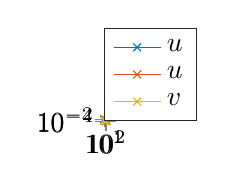
\begin{tikzpicture}

\begin{axis}[%
width=0.951\figwidth,
height=0.75\figwidth,
at={(0\figwidth,0\figwidth)},
scale only axis,
xmode=log,
xmin=4,
xmax=100,
xminorticks=true,
ymode=log,
ymin=1e-05,
ymax=0.1,
yminorticks=true,
axis background/.style={fill=white},
legend style={at={(0.03,0.03)}, anchor=south west, legend cell align=left, align=left, draw=white!15!black}
]
\addplot [color=mycolor1, mark=x, mark options={solid, mycolor1}]
  table[row sep=crcr]{%
4	0.0377253281\\
8	0.016292839\\
16	0.00647505826\\
32	0.00277859939\\
64	0.00131783073\\
};
\addlegendentry{$u$}

\addplot [color=mycolor2, mark=x, mark options={solid, mycolor2}]
  table[row sep=crcr]{%
4	0.00100309389\\
8	0.000409725552\\
16	0.000134946447\\
32	5.06672786e-05\\
64	2.29407924e-05\\
};
\addlegendentry{$u$}

\addplot [color=mycolor3, mark=x, mark options={solid, mycolor3}]
  table[row sep=crcr]{%
4	0.000631316968\\
8	0.000278812074\\
16	0.00010907144\\
32	4.76177485e-05\\
64	2.28652417e-05\\
};
\addlegendentry{$v$}

\addplot [color=white!70!black, forget plot]
  table[row sep=crcr]{%
4	0.00025\\
100	1e-05\\
};
\addplot [color=white!70!black, forget plot]
  table[row sep=crcr]
	\subfloat[Upwind, $Re = \num{e3}$]{
		\input{../img/l2error_test_navierstokes_sincos_hre}}\\
	\subfloat[Min-Mod, $Re = 1$]{
		% This file was created by matlab2tikz.
%
\definecolor{mycolor1}{rgb}{0.00000,0.44700,0.74100}%
\definecolor{mycolor2}{rgb}{0.85000,0.32500,0.09800}%
\definecolor{mycolor3}{rgb}{0.92900,0.69400,0.12500}%
%
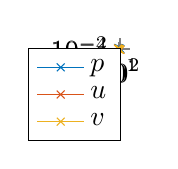
\begin{tikzpicture}

\begin{axis}[%
width=0.951\figwidth,
height=0.75\figwidth,
at={(0\figwidth,0\figwidth)},
scale only axis,
xmode=log,
xmin=4,
xmax=100,
xminorticks=true,
ymode=log,
ymin=1e-05,
ymax=0.1,
yminorticks=true,
axis background/.style={fill=white},
legend style={at={(0.97,0.97)}, anchor=north east, legend cell align=left, align=left}
]
\addplot [color=mycolor1, mark=x, mark options={solid, mycolor1}]
  table[row sep=crcr]{%
4	0.0201961443\\
8	0.00658170291\\
16	0.00181646151\\
32	0.000558641084\\
64	0.000188245776\\
};
\addlegendentry{$p$}

\addplot [color=mycolor2, mark=x, mark options={solid, mycolor2}]
  table[row sep=crcr]{%
4	0.00148598782\\
8	0.00053497283\\
16	0.000150385476\\
32	3.95894587e-05\\
64	1.01636468e-05\\
};
\addlegendentry{$u$}

\addplot [color=mycolor3, mark=x, mark options={solid, mycolor3}]
  table[row sep=crcr]{%
4	0.00119526142\\
8	0.00045470553\\
16	0.000138075359\\
32	3.80865907e-05\\
64	1.00057526e-05\\
};
\addlegendentry{$v$}

\addplot [color=white!70!black, forget plot]
  table[row sep=crcr]{%
4	0.00025\\
100	1e-05\\
};
\addplot [color=white!70!black, forget plot]
  table[row sep=crcr]
	\subfloat[Min-Mod, $Re = \num{e3}$]{
		\input{../img/l2error_test_navierstokes_sincos_mm_hre}}\\
	\subfloat[Van Leer, $Re = 1$]{
		% This file was created by matlab2tikz.
%
\definecolor{mycolor1}{rgb}{0.00000,0.44700,0.74100}%
\definecolor{mycolor2}{rgb}{0.85000,0.32500,0.09800}%
\definecolor{mycolor3}{rgb}{0.92900,0.69400,0.12500}%
%
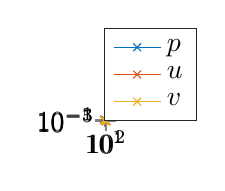
\begin{tikzpicture}

\begin{axis}[%
width=0.951\figwidth,
height=0.75\figwidth,
at={(0\figwidth,0\figwidth)},
scale only axis,
xmode=log,
xmin=4,
xmax=100,
xminorticks=true,
ymode=log,
ymin=8.63199669e-06,
ymax=0.1,
yminorticks=true,
axis background/.style={fill=white},
legend style={at={(0.03,0.03)}, anchor=south west, legend cell align=left, align=left, draw=white!15!black}
]
\addplot [color=mycolor1, mark=x, mark options={solid, mycolor1}]
  table[row sep=crcr]{%
4	0.017335487\\
8	0.0062618753\\
16	0.00193371119\\
32	0.000605597659\\
64	0.000196206927\\
};
\addlegendentry{$p$}

\addplot [color=mycolor2, mark=x, mark options={solid, mycolor2}]
  table[row sep=crcr]{%
4	0.00136409678\\
8	0.000476275877\\
16	0.000131606902\\
32	3.41242821e-05\\
64	8.66824542e-06\\
};
\addlegendentry{$u$}

\addplot [color=mycolor3, mark=x, mark options={solid, mycolor3}]
  table[row sep=crcr]{%
4	0.00114596769\\
8	0.000417513208\\
16	0.000122988533\\
32	3.32359157e-05\\
64	8.63199669e-06\\
};
\addlegendentry{$v$}

\addplot [color=white!70!black, forget plot]
  table[row sep=crcr]{%
4	0.00021579991725\\
100	8.63199669e-06\\
};
\addplot [color=white!70!black, forget plot]
  table[row sep=crcr]
	\subfloat[Van Leer, $Re = \num{e3}$]{
		% This file was created by matlab2tikz.
%
\definecolor{mycolor1}{rgb}{0.00000,0.44700,0.74100}%
\definecolor{mycolor2}{rgb}{0.85000,0.32500,0.09800}%
\definecolor{mycolor3}{rgb}{0.92900,0.69400,0.12500}%
%
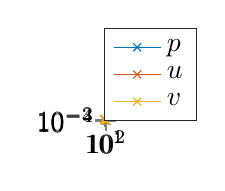
\begin{tikzpicture}

\begin{axis}[%
width=0.951\figwidth,
height=0.75\figwidth,
at={(0\figwidth,0\figwidth)},
scale only axis,
xmode=log,
xmin=4,
xmax=100,
xminorticks=true,
ymode=log,
ymin=0.0001,
ymax=0.01454297,
yminorticks=true,
axis background/.style={fill=white},
legend style={at={(0.03,0.03)}, anchor=south west, legend cell align=left, align=left, draw=white!15!black}
]
\addplot [color=mycolor1, mark=x, mark options={solid, mycolor1}]
  table[row sep=crcr]{%
4	0.01454297\\
8	0.00653869074\\
16	0.00224775854\\
32	0.0005196908\\
64	0.000249600967\\
};
\addlegendentry{$p$}

\addplot [color=mycolor2, mark=x, mark options={solid, mycolor2}]
  table[row sep=crcr]{%
4	0.0107200353\\
8	0.00466675248\\
16	0.00177426299\\
32	0.000645881865\\
64	0.000238530337\\
};
\addlegendentry{$u$}

\addplot [color=mycolor3, mark=x, mark options={solid, mycolor3}]
  table[row sep=crcr]{%
4	0.0112112271\\
8	0.00583504088\\
16	0.00263953931\\
32	0.00102531826\\
64	0.000347747564\\
};
\addlegendentry{$v$}

\addplot [color=white!70!black, forget plot]
  table[row sep=crcr]{%
4	0.0025\\
100	0.0001\\
};
\addplot [color=white!70!black, forget plot]
  table[row sep=crcr]{%
4	0.0625\\
100	0.0001\\
};
\end{axis}
\end{tikzpicture}%\label{fig:sin_err_vl_hre}}
	\caption[$L^2(\Omega)$ norm of the errors for the Sin-Cos 
	test]{$L^2(\Omega)$ norm of the errors 
	for the Sin-Cos 
	test depending on the square root of the number of cells in the grid. 
	The grey lines are the reference lines parallel to a first order convergence (the lower one) and a
	second order convergence (the upper one).}
	\label{fig:sin_err}
\end{figure}

\begin{table}
	\centering
	\subfloat[][$Re=1$]{
	$\begin{array}{c|ccc}
	\toprule
	& \text{Upwind} & \text{Min-Mod} & \text{Van Leer} \\ 
	\midrule
	p & 1.008 & 1.569 & 1.626\\
	u & 1.143 & 1.962 & 1.977\\
	v & 1.058 & 1.928 & 1.945\\
	\bottomrule
	\end{array}
	\label{tab:sin_lre}$
	}\\
	\subfloat[][$Re=\num{e3}$]{
	$\begin{array}{c|ccc}
	\toprule
	& \text{Upwind} & \text{Min-Mod} & \text{Van Leer} \\ 
	\midrule
	p & 1.148 & 1.659 & 1.058\\
	u & 1.071 & 1.441 & 1.437\\
	v & 1.068 & 1.533 & 1.560\\
	\bottomrule
	\end{array}
	\label{tab:sin_hre}$
	}
	\caption[Convergence orders for the Sin-Cos test]{Convergence orders for 
	the Sin-Cos test. They are computed considering the last two refinements of 
	the grid.}
	\label{tab:sin_conv}
\end{table}

We observe, as expected, a better behaviour of the TVD methods with respect to 
the upwind method. In Table~\ref{tab:sin_lre}, we can see that, at $Re=1$, the 
formers show a full second order convergence for the velocity, while for the pressure the
rate is a bit lower; the latter, instead, shows a first order convergence for 
all variables. At 
$Re=\num{e3}$, a slight decrease of the rates of the TVD methods occurs also 
for 
the velocities, but they remain higher then the ones of the upwind method. In 
Table~\ref{tab:sin_hre}, we observe a convergence order of 1 for the pressure 
using the Van Leer flux limiter, but, looking at 
Figure~\ref{fig:sin_err_vl_hre}, we can 
see that the global trend points to a convergence of higher order. Moreover, it 
can be observed how, thanks to the faster convergence, on the same grid the 
absolute values of the errors reach smaller values using the TVD methods. 
Between the Min-Mod and Van Leer flux limiters it is hard to say which one 
performs better. The results are very similar.

Analogous tests with other analytical solutions are reported in 
Appendix~\ref{app:conv}. They show always a better convergence of the TVD 
methods with respect to the upwind method, but in some cases the convergence 
order of pressure and velocity behave differently.
%
\subsection{Time convergence}
We test the time convergence of the $L^\infty(0,T;L^2(\Omega))$ norm of the 
error of the solution of the Navier-Stokes equations:
\begin{equation}
	|\!|\phi_\text{ex}-\phi_h|\!|_{L^\infty(0,T;L^2(\Omega))} = \esssup_{t \in 
	(0,T)} |\!|\phi_\text{ex}(t) - \phi_h(t) |\!|_{L^2(\Omega)}, 
\end{equation}
where $\esssup$ denotes the \emph{essential supremum}, that for a function 
$f:\Omega\rightarrow\mathbb{R}$ is defined as
\begin{equation}
	\esssup_\Omega f = \inf \{\text{$M \in \mathbb{R}$ : $ |f(x)| \leq 
	M$ a.e. in $\Omega$} \}.
\end{equation}
In our case it will be the maximum of the $L^2(\Omega)$ norm of error over the 
time interval $(0,T)$. We compare the results 
obtained with the BE method \eqref{eq:be} and the BDF2 method \eqref{eq:bdf2}.\\
We consider the unsteady version of the 
equations~\eqref{eq:nssteadymass}--\eqref{eq:nssteadymom}:
\begin{align}
	\label{eq:nsunsteadymass} \nabla \cdot \mathbf{v} -h = 0&\\
	\label{eq:nsunsteadymom} \frac{\partial \mathbf{v}}{\partial t} +\nabla 
	\cdot (\mathbf{v} \mathbf{v}^\mathrm{T}) - 
	\nabla \cdot (\nu \nabla \mathbf{v}) + \frac{1}{\varrho}\nabla p  
	-\mathbf{f} = \mathbf{0}&
\end{align}
Again the gravity is neglected and two possible sources $h$ and $\mathbf{f}$ 
are taken into account, moreover all the quantities are considered to be 
non-dimensional.
%
\subsubsection{Unsteady Sin-Cos test}
Let us solve the equations~\eqref{eq:nsunsteadymass}--\eqref{eq:nsunsteadymom} 
over a two dimensional unit domain $\Omega=(0,1)^2$ and in the time interval 
$(0,T)$, with $T=1$. We use the following source terms:
\begin{align}
h &= 0,\\
\mathbf{f} &= 2\Big(\frac{\cos(2t)}{\varrho} + \nu \sin(2t)\Big)[- \cos(x) 
\sin(y), \; 
\cos(y) \sin(x)]^\mathrm{T},
\end{align}
so that, choosing $\varrho=1$, the analytical solution is given by
\begin{align}
\label{eq:uexunssin}	u_\text{ex}(x,y) &= -\cos(x)\sin(y)\sin(2t),\\
v_\text{ex}(x,y) &= \sin(x)\cos(y)\sin(2t),\\
\label{eq:pexunssin}	p_\text{ex}(x,y) &= 
-\frac{\cos(2x)+\sin(2y)}{4}\sin^2(2t).
\end{align}
It is equal to \eqref{eq:uexsin}--\eqref{eq:pexsin}, used in the steady test 
for the space convergence, except for the modulation over time. We choose 
$\nu=0.1$, so that $Re=10$. Dirichlet boundary conditions for the velocity are 
applied on the whole boundary $\partial \Omega$ using the exact solution. 
The pressure is again fixed  at one point in order to match the particular exact solution 
\eqref{eq:pexunssin}.

The problem is solved seven times subdividing the time interval $(0,T)$ into 
uniform time-steps and each time doubling their number, starting from a 
discretization with a
single time-step. Uniform grids of $\num{40x40}$ and $\num{80x80}$ cells are 
employed and, as a differencing scheme, the TVD method with the Van Leer flux 
limiter \eqref{eq:vl} is used. From Figure~\ref{fig:timeerr}, we observe that, 
as expected, the BE method shows a first order convergence, while the BDF2 
method is of second order. Moreover we notice that, with a grid of 
$\num{40x40}$ cells, in the last refinement the error with the BDF2 method does 
not decrease anymore. This happens because the grid is too coarse and the 
spatial error becomes dominant over the temporal one, so that, even with small 
time-steps, we can not improve the solution.
Refining the grid, the spatial error is reduced and the temporal order of convergence is restored entirely for the pressure and almost for the velocity.
\begin{figure}
	\centering
	\subfloat{\input{../img/time_convergence_p_report}}
	\subfloat{% This file was created by matlab2tikz.
%
\definecolor{mycolor1}{rgb}{0.00000,0.44700,0.74100}%
\definecolor{mycolor2}{rgb}{0.85000,0.32500,0.09800}%
\definecolor{mycolor3}{rgb}{0.92900,0.69400,0.12500}%
%
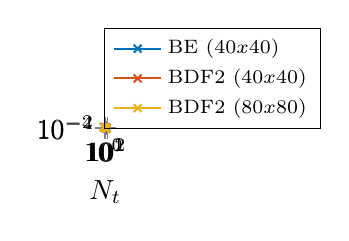
\begin{tikzpicture}

\begin{axis}[%
width=0.99\figwidth,
height=0.8\figwidth,
at={(0\figwidth,0\figwidth)},
scale only axis,
xmode=log,
xmin=1,
xmax=100,
xminorticks=true,
xlabel={$N_t$},
ymode=log,
ymin=1e-5,
ymax=1e-1,
yminorticks=true,
%ylabel style={font=\scriptsize},
%ylabel={$L^\infty$-error},
axis background/.style={fill=white},
legend style={at={(0.03,0.03)}, anchor=south west, legend cell align=left, fill=none,
align=left, font=\scriptsize}
]

\addplot [color=white!70!black, forget plot, line width=0.75pt]
  table[row sep=crcr]{%
1	0.1\\
100	0.001\\
};
\addplot [color=white!70!black, forget plot, line width=0.75pt]
  table[row sep=crcr]{%
1	0.1\\
100	0.00001\\
};
\addplot [color=mycolor1, mark=x, mark options={solid, mycolor1}, line width=0.75pt]
  table[row sep=crcr]{%
1	5.516e-2\\
2	3.043e-2\\
4	1.607e-2\\
8	8.216e-3\\
16	4.12e-3\\
32	2.03e-3\\
64	9.712e-4\\
};
\addlegendentry{BE ($\num{40x40}$)}

\addplot [color=mycolor2, mark=x, mark options={solid, mycolor2}, line width=0.75pt]
  table[row sep=crcr]{%
1	5.516e-2\\
2	1.645e-2\\
4	4.8e-3\\
8	1.21e-3\\
16	2.85e-4\\
32	1.3e-4\\
64	1.278e-4\\
};
\addlegendentry{BDF2 ($\num{40x40}$)}

\addplot [color=mycolor3, mark=x, mark options={solid, mycolor3}, line width=0.75pt]
  table[row sep=crcr]
	\caption[$L^\infty(0,T;L^2(\Omega))$ norm of the errors for the unsteady 
	Sin-Cos 
	test]{$L^\infty(0,T;L^2(\Omega))$ norm of the errors for the unsteady 
	Sin-Cos test 
	depending on the number of time-steps. On the left the errors for the 
	pressure, on the right the errors for the magnitude of the velocity. The grey lines are the reference lines parallel to a first order convergence (the lower one) and a
	second order convergence (the upper one).}
	\label{fig:timeerr}
\end{figure}
%
\subsection{Rough channel test} \label{subsec:roughchannel}
We test the behaviour of the TVD methods compared to the upwind method solving 
the unsteady Navier-Stokes equations \eqref{eq:nsmass}--\eqref{eq:nsmom} in 
a two-dimensional channel with a \emph{rough} (i.e. non-flat) lower boundary that 
consists of small, evenly spaced cavities. Two different 
configurations are studied, one with shallow cavities, depicted in 
Figure~\ref{fig:roughdom}, and another with deeper cavities, depicted in 
Figure~\ref{fig:roughdomdeep}.

On the left boundary $\Gamma_\text{in}$ we set inflow boundary conditions 
\eqref{eq:inflow}, specifying a horizontal velocity
\begin{equation}
	\mathbf{v} = \mathbf{v}_\text{in} = [u_\text{in}, 0]^\mathrm{T}, \quad 
	u_\text{in} = \SI{1}{m/s}.
\end{equation}
On the lower and upper boundaries $\Gamma_w$, we set no-slip boundary 
conditions 
\eqref{eq:noslip}, while on the right boundary $\Gamma_\text{out}$ we set 
outflow boundary conditions \eqref{eq:outflow}, fixing the value of the pressure
\begin{equation}
	p = p_\text{ext} = \SI{1.1e5}{\pascal}.
\end{equation}
As initial conditions, velocity is set to zero everywhere, while pressure is 
set to $p_\text{ext}$ everywhere. Density is 
$\varrho=\SI{1}{kg/m^3}$. The gravity contribution in \eqref{eq:nsmom} is 
neglected.
%
\subsubsection{Shallow cavities}
In the case of shallow cavities we use the domain in Figure~\ref{fig:roughdom} 
and we employ a uniform grid of $\num{95x50}$ cells. The problem is then solved 
over the time interval ($0,T$), with $T=\SI{10}{s}$. The initial time-step is 
$\Delta t=\SI{5e-3}{s}$, then it is adapted as explained in 
Section~\ref{sec:algeq}, allowing a maximum time-step of $\SI{0.1}{s}$. 
At first we set $\nu=\SI{5e-4}{m^2/s}$, so that $Re=\num{2e3}$. Since we do not 
have an analytical solution for this problem, we compute a \emph{reference 
solution} using the upwind method over a grid six times finer (see Figure~\ref{fig:roughchannelgrid}).

In Figure~\ref{fig:linecompshallow} we compare the profiles of the magnitude 
of the velocity along a cross-section near the end of the channel, at 
$x=\SI{8.75}{m}$, i.e. at the middle of the last cavity.  The TVD solutions 
match the reference case, while the upwind solution shows a small shift, 
especially in the lower part of the channel, above the cavity. In 
Table~\ref{tab:errshallow}, we can see the 
$L^2(\Omega)$ norm 
of the errors of the coarse solutions computed with respect to the reference 
one, along the cross-section mentioned above. The one related to the 
upwind method is at least one order of magnitude larger than the others. 
\begin{figure}
	\centering
	\includegraphics[width=\textwidth]{rough_domain2.pdf}
	\caption[Domain of the rough channel test with shallow cavities]{Domain of 
	the rough channel test with shallow cavities.}
	\label{fig:roughdom}
\end{figure}
\begin{figure}
	\centering
	\includegraphics[width=\textwidth]{rough_channel_vl_report.png}
	\caption[Magnitude of the velocity in the rough channel test with 
	shallow cavities]{Magnitude of the velocity $[\si{m/s}]$ in the 
	rough channel test with shallow cavities at $t=T$. $Re=\num{2e3}$. 
	Van Leer flux limiter.}
	\label{fig:roughchannelvl}
\end{figure}
% Nuova figura:
\begin{figure}
	\centering
	\includegraphics[width=\textwidth, trim={0 0 0 1.5cm}, clip]{rough_channel_one_step_arrows.png}
	\caption[Magnitude of the velocity in the rough channel test with schallo cavities around the last cavity]{Magnitude of the velocity $[\si{m/s}]$ in the rough channel test with shallow cavities, around the last cavity, at $t=T$, in the reference case. $Re=\num{2e3}$. The arrows are not scaled.}
\end{figure}
\begin{figure}
	\centering
	\includegraphics[width=\textwidth]{rough_channel_grid.pdf}
	\caption[Grid comparison in the rough channel test]{Comparison of the grids used in the rough channel test. In black the grid used for the reference solution, with cell sizes $\SI{16.7x3.3}{mm}$, in blue the grid used in the other simulations, with cell sizes $\SI{100x20}{mm}$.}
	\label{fig:roughchannelgrid}
\end{figure}
\begin{figure}
	\centering
	% This file was created by matlab2tikz.
%
\definecolor{mycolor1}{rgb}{0.00000,0.44700,0.74100}%
\definecolor{mycolor2}{rgb}{0.85000,0.32500,0.09800}%
\definecolor{mycolor3}{rgb}{0.92900,0.69400,0.12500}%
\definecolor{mycolor4}{rgb}{0.49400,0.18400,0.55600}%
%
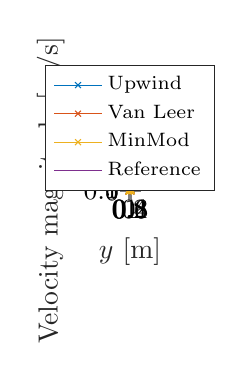
\begin{tikzpicture}

\begin{axis}[%
width=0.951\roughwidth,
height=0.75\roughheight,
at={(0\roughwidth,0\roughheight)},
scale only axis,
xmin=0,
xmax=1,
xlabel style={font=\color{white!15!black}},
xlabel={$y$ [m]},
ymin=0,
ymax=1.25,
ylabel style={font=\color{white!15!black}},
ylabel={Velocity magnitude [m/s]},
axis background/.style={fill=white},
legend style={at={(0.5,0.03)}, anchor=south, legend cell align=left, align=left, draw=white!15!black, font=\scriptsize}
]
\addplot [color=mycolor1, mark size=1.5pt, mark=x, mark options={solid, mycolor1}]
  table[row sep=crcr]{%
0	0\\
0.01	0.0293662\\
0.03	0.050586\\
0.05	0.0374104\\
0.07	0.00830816\\
0.09	0.0878588\\
0.11	0.203537\\
0.13	0.350154\\
0.15	0.504986\\
0.17	0.648407\\
0.19	0.773425\\
0.21	0.879108\\
0.23	0.965875\\
0.25	1.0347\\
0.27	1.08726\\
0.29	1.12581\\
0.31	1.15286\\
0.33	1.17097\\
0.35	1.18249\\
0.37	1.18938\\
0.39	1.19321\\
0.41	1.19513\\
0.43	1.19595\\
0.45	1.19618\\
0.47	1.19615\\
0.49	1.19606\\
0.51	1.19602\\
0.53	1.19608\\
0.55	1.19627\\
0.57	1.19661\\
0.59	1.19708\\
0.61	1.1977\\
0.63	1.19842\\
0.65	1.19918\\
0.67	1.19986\\
0.69	1.20024\\
0.71	1.19994\\
0.73	1.19831\\
0.75	1.19437\\
0.77	1.18669\\
0.79	1.17327\\
0.81	1.15154\\
0.83	1.11834\\
0.85	1.07018\\
0.87	1.00343\\
0.89	0.914856\\
0.91	0.802051\\
0.93	0.663892\\
0.95	0.500819\\
0.97	0.314904\\
0.99	0.109749\\
1	0\\
};
\addlegendentry{Upwind}

\addplot [color=mycolor2, mark size=1.5pt, mark=x, mark options={solid, mycolor2}]
  table[row sep=crcr]{%
0	0\\
0.01	0.0271697\\
0.03	0.0500789\\
0.05	0.0401093\\
0.07	0.00567534\\
0.09	0.0811925\\
0.11	0.199174\\
0.13	0.35443\\
0.15	0.52202\\
0.17	0.675188\\
0.19	0.804904\\
0.21	0.91139\\
0.23	0.996051\\
0.25	1.06075\\
0.27	1.10807\\
0.29	1.14103\\
0.31	1.16275\\
0.33	1.17616\\
0.35	1.18381\\
0.37	1.1877\\
0.39	1.18933\\
0.41	1.18969\\
0.43	1.18942\\
0.45	1.18894\\
0.47	1.18845\\
0.49	1.18804\\
0.51	1.18779\\
0.53	1.1877\\
0.55	1.18779\\
0.57	1.18804\\
0.59	1.18848\\
0.61	1.18909\\
0.63	1.18985\\
0.65	1.19073\\
0.67	1.19161\\
0.69	1.19229\\
0.71	1.1924\\
0.73	1.19132\\
0.75	1.18802\\
0.77	1.181\\
0.79	1.16815\\
0.81	1.14675\\
0.83	1.11359\\
0.85	1.06512\\
0.87	0.997859\\
0.89	0.908818\\
0.91	0.795828\\
0.93	0.657971\\
0.95	0.495791\\
0.97	0.311428\\
0.99	0.10845\\
1	0\\
};
\addlegendentry{Van Leer}

\addplot [color=mycolor3, mark size=1.5pt, mark=x, mark options={solid, mycolor3}]
  table[row sep=crcr]{%
0	0\\
0.01	0.0272093\\
0.03	0.0494723\\
0.05	0.0389859\\
0.07	0.00595636\\
0.09	0.0812851\\
0.11	0.198804\\
0.13	0.353914\\
0.15	0.5204\\
0.17	0.672249\\
0.19	0.801321\\
0.21	0.907555\\
0.23	0.992249\\
0.25	1.05727\\
0.27	1.10509\\
0.29	1.13867\\
0.31	1.16106\\
0.33	1.17513\\
0.35	1.18335\\
0.37	1.18771\\
0.39	1.18968\\
0.41	1.19029\\
0.43	1.19022\\
0.45	1.18987\\
0.47	1.18946\\
0.49	1.18912\\
0.51	1.18891\\
0.53	1.18887\\
0.55	1.18899\\
0.57	1.18928\\
0.59	1.18974\\
0.61	1.19035\\
0.63	1.19112\\
0.65	1.19197\\
0.67	1.19282\\
0.69	1.19344\\
0.71	1.19347\\
0.73	1.19226\\
0.75	1.18881\\
0.77	1.18163\\
0.79	1.16863\\
0.81	1.14714\\
0.83	1.11395\\
0.85	1.06554\\
0.87	0.998402\\
0.89	0.90948\\
0.91	0.796585\\
0.93	0.658719\\
0.95	0.496437\\
0.97	0.311872\\
0.99	0.108614\\
1	0\\
};
\addlegendentry{MinMod}

\addplot [color=mycolor4]
  table[row sep=crcr]{%
0	0\\
0.00166667	0.00492427\\
0.005	0.0138838\\
0.00833333	0.0219483\\
0.0116667	0.0291114\\
0.015	0.0353663\\
0.0183333	0.0407062\\
0.0216667	0.0451241\\
0.025	0.0486134\\
0.0283333	0.051167\\
0.0316667	0.0527786\\
0.035	0.0534416\\
0.0383333	0.0531503\\
0.0416667	0.0518985\\
0.045	0.0496806\\
0.0483333	0.0464911\\
0.0516667	0.042324\\
0.055	0.037174\\
0.0583333	0.0310358\\
0.0616667	0.0239061\\
0.065	0.0157914\\
0.0683333	0.00678684\\
0.0716667	0.00421506\\
0.075	0.0150977\\
0.0783333	0.0273447\\
0.0816667	0.0407005\\
0.085	0.0551595\\
0.0883333	0.0707355\\
0.0916667	0.0874415\\
0.095	0.105279\\
0.0983333	0.124233\\
0.101667	0.144291\\
0.105	0.165438\\
0.108333	0.187646\\
0.111667	0.210875\\
0.115	0.23507\\
0.118333	0.260158\\
0.121667	0.286047\\
0.125	0.312628\\
0.128333	0.33978\\
0.131667	0.367367\\
0.135	0.395245\\
0.138333	0.42327\\
0.141667	0.451298\\
0.145	0.479192\\
0.148333	0.506829\\
0.151667	0.534103\\
0.155	0.560921\\
0.158333	0.587212\\
0.161667	0.612919\\
0.165	0.638002\\
0.168333	0.662436\\
0.171667	0.686204\\
0.175	0.7093\\
0.178333	0.731723\\
0.181667	0.753476\\
0.185	0.774566\\
0.188333	0.795\\
0.191667	0.814784\\
0.195	0.833928\\
0.198333	0.852438\\
0.201667	0.870321\\
0.205	0.887585\\
0.208333	0.904234\\
0.211667	0.920276\\
0.215	0.935716\\
0.218333	0.950561\\
0.221667	0.964818\\
0.225	0.978495\\
0.228333	0.991598\\
0.231667	1.00414\\
0.235	1.01612\\
0.238333	1.02756\\
0.241667	1.03847\\
0.245	1.04885\\
0.248333	1.05871\\
0.251667	1.06808\\
0.255	1.07696\\
0.258333	1.08537\\
0.261667	1.09332\\
0.265	1.10082\\
0.268333	1.10789\\
0.271667	1.11454\\
0.275	1.12079\\
0.278333	1.12664\\
0.281667	1.13213\\
0.285	1.13725\\
0.288333	1.14203\\
0.291667	1.14648\\
0.295	1.15062\\
0.298333	1.15445\\
0.301667	1.158\\
0.305	1.16127\\
0.308333	1.16429\\
0.311667	1.16706\\
0.315	1.1696\\
0.318333	1.17192\\
0.321667	1.17404\\
0.325	1.17597\\
0.328333	1.17771\\
0.331667	1.17929\\
0.335	1.18071\\
0.338333	1.18198\\
0.341667	1.18311\\
0.345	1.18412\\
0.348333	1.18501\\
0.351667	1.18579\\
0.355	1.18647\\
0.358333	1.18706\\
0.361667	1.18757\\
0.365	1.188\\
0.368333	1.18836\\
0.371667	1.18866\\
0.375	1.1889\\
0.378333	1.18908\\
0.381667	1.18923\\
0.385	1.18933\\
0.388333	1.18939\\
0.391667	1.18942\\
0.395	1.18942\\
0.398333	1.1894\\
0.401667	1.18935\\
0.405	1.18928\\
0.408333	1.1892\\
0.411667	1.18911\\
0.415	1.189\\
0.418333	1.18888\\
0.421667	1.18876\\
0.425	1.18863\\
0.428333	1.18849\\
0.431667	1.18836\\
0.435	1.18822\\
0.438333	1.18808\\
0.441667	1.18794\\
0.445	1.1878\\
0.448333	1.18766\\
0.451667	1.18753\\
0.455	1.1874\\
0.458333	1.18727\\
0.461667	1.18715\\
0.465	1.18703\\
0.468333	1.18691\\
0.471667	1.1868\\
0.475	1.1867\\
0.478333	1.1866\\
0.481667	1.18651\\
0.485	1.18642\\
0.488333	1.18634\\
0.491667	1.18626\\
0.495	1.18619\\
0.498333	1.18613\\
0.501667	1.18607\\
0.505	1.18601\\
0.508333	1.18597\\
0.511667	1.18593\\
0.515	1.18589\\
0.518333	1.18586\\
0.521667	1.18584\\
0.525	1.18582\\
0.528333	1.18581\\
0.531667	1.1858\\
0.535	1.1858\\
0.538333	1.18581\\
0.541667	1.18582\\
0.545	1.18584\\
0.548333	1.18586\\
0.551667	1.18589\\
0.555	1.18593\\
0.558333	1.18597\\
0.561667	1.18602\\
0.565	1.18607\\
0.568333	1.18613\\
0.571667	1.18619\\
0.575	1.18626\\
0.578333	1.18634\\
0.581667	1.18642\\
0.585	1.18651\\
0.588333	1.1866\\
0.591667	1.1867\\
0.595	1.18681\\
0.598333	1.18692\\
0.601667	1.18703\\
0.605	1.18716\\
0.608333	1.18729\\
0.611667	1.18742\\
0.615	1.18756\\
0.618333	1.18771\\
0.621667	1.18786\\
0.625	1.18802\\
0.628333	1.18819\\
0.631667	1.18835\\
0.635	1.18853\\
0.638333	1.18871\\
0.641667	1.18889\\
0.645	1.18908\\
0.648333	1.18927\\
0.651667	1.18947\\
0.655	1.18967\\
0.658333	1.18987\\
0.661667	1.19007\\
0.665	1.19028\\
0.668333	1.19048\\
0.671667	1.19068\\
0.675	1.19089\\
0.678333	1.19108\\
0.681667	1.19128\\
0.685	1.19147\\
0.688333	1.19165\\
0.691667	1.19182\\
0.695	1.19197\\
0.698333	1.19212\\
0.701667	1.19224\\
0.705	1.19235\\
0.708333	1.19243\\
0.711667	1.19249\\
0.715	1.19252\\
0.718333	1.19251\\
0.721667	1.19246\\
0.725	1.19237\\
0.728333	1.19223\\
0.731667	1.19204\\
0.735	1.19178\\
0.738333	1.19146\\
0.741667	1.19107\\
0.745	1.19059\\
0.748333	1.19003\\
0.751667	1.18937\\
0.755	1.1886\\
0.758333	1.18772\\
0.761667	1.18671\\
0.765	1.18557\\
0.768333	1.18428\\
0.771667	1.18283\\
0.775	1.18122\\
0.778333	1.17942\\
0.781667	1.17743\\
0.785	1.17523\\
0.788333	1.17282\\
0.791667	1.17016\\
0.795	1.16726\\
0.798333	1.16409\\
0.801667	1.16064\\
0.805	1.15689\\
0.808333	1.15283\\
0.811667	1.14845\\
0.815	1.14372\\
0.818333	1.13862\\
0.821667	1.13315\\
0.825	1.12728\\
0.828333	1.12101\\
0.831667	1.1143\\
0.835	1.10714\\
0.838333	1.09953\\
0.841667	1.09143\\
0.845	1.08284\\
0.848333	1.07374\\
0.851667	1.06411\\
0.855	1.05394\\
0.858333	1.04321\\
0.861667	1.0319\\
0.865	1.02002\\
0.868333	1.00753\\
0.871667	0.994433\\
0.875	0.980713\\
0.878333	0.96636\\
0.881667	0.951363\\
0.885	0.935712\\
0.888333	0.919401\\
0.891667	0.90242\\
0.895	0.884765\\
0.898333	0.866428\\
0.901667	0.847407\\
0.905	0.827698\\
0.908333	0.807298\\
0.911667	0.786206\\
0.915	0.764423\\
0.918333	0.74195\\
0.921667	0.718789\\
0.925	0.694943\\
0.928333	0.670418\\
0.931667	0.645219\\
0.935	0.619353\\
0.938333	0.592828\\
0.941667	0.565653\\
0.945	0.537839\\
0.948333	0.509397\\
0.951667	0.48034\\
0.955	0.45068\\
0.958333	0.420433\\
0.961667	0.389615\\
0.965	0.358241\\
0.968333	0.326328\\
0.971667	0.293895\\
0.975	0.260961\\
0.978333	0.227546\\
0.981667	0.193668\\
0.985	0.15935\\
0.988333	0.124612\\
0.991667	0.0894758\\
0.995	0.0539638\\
0.998333	0.0180982\\
1	0\\
};
\addlegendentry{Reference}
\addplot [color=black, dashed]
  table[row sep=crcr]{%
0.1	0\\
0.1 1.25\\
};
\end{axis}
\end{tikzpicture}%
	\caption[Profile of the magnitude of the velocity in the rough channel with 
	shallow cavities at $Re=\num{2e3}$]{Profile of the magnitude of the 
	velocity $[\si{m/s}]$ in the rough channel with shallow cavities along the 
	cross-section $x=\SI{8.75}{m}$, at $t=T$. $Re=\num{2e3}$. The region on 
	the left of the dashed line is inside the cavity.}
	\label{fig:linecompshallow}
\end{figure}
\begin{table}
	\centering
	\[
	\begin{array}{ccc}
	\toprule
	\text{Upwind} & \text{Van Leer} & \text{Van Alabada} \\
	\midrule
	\num{1.708e-4} & \num{9.556e-6} & \num{1.119e-5} \\
	\midrule
	\text{Min-Mod} & \text{Superbee} & \text{MC Limiter} \\
	\midrule
	\num{1.537e-5} &  \SI{8.335e-6} & \num{8.659e-6}\\
	\bottomrule
	\end{array}
	\]
	\caption[$L^2(\Omega)$ norm of the errors for the profile of the magnitude 
	of the 
	velocity in 
	the rough channel with shallow cavities at 
	$Re=\num{2e3}$]{$L^2(\Omega)$ norm of the errors for 
	the profile of the magnitude of the velocity along the cross-section at 
	$x=\SI{8.75}{m}$ and $t=T$ in the rough channel with shallow 
	cavities. $Re = \num{2e3}$.}
	\label{tab:errshallow}
\end{table}

We repeat the test choosing $\nu=\SI{1}{m^2/s}$, so that $Re=1$. In 
Figure~\ref{fig:linecompshallowlre} we see that all the solutions have the same 
profile, moreover in the cavity there is not any recirculation. In 
Table~\ref{tab:errshallow_lre} the $L^2(\Omega)$ norm of the errors are 
reported; the 
upwind one is 
the bigger, but they are all very similar. So, in this situation of low $Re$, 
being the results very similar, the benefit of using a high-resolution scheme 
is reduced.
\begin{figure}
	\centering
	% This file was created by matlab2tikz.
%
\definecolor{mycolor1}{rgb}{0.00000,0.44700,0.74100}%
\definecolor{mycolor2}{rgb}{0.85000,0.32500,0.09800}%
\definecolor{mycolor3}{rgb}{0.92900,0.69400,0.12500}%
\definecolor{mycolor4}{rgb}{0.49400,0.18400,0.55600}%
%
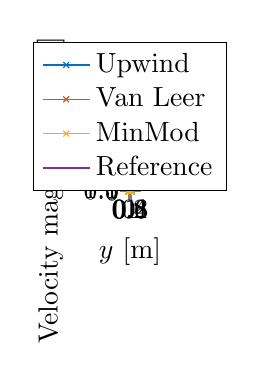
\begin{tikzpicture}

\begin{axis}[%
width=0.951\roughwidth,
height=0.75\roughheight,
at={(0\roughwidth,0\roughheight)},
scale only axis,
xmin=0,
xmax=1,
xlabel={$y$ [m]},
ymin=0,
ymax=1.5,
ylabel={Velocity magnitude [m/s]},
axis background/.style={fill=white},
legend style={at={(0.5,0.03)}, anchor=south, legend cell align=left, align=left}
]
\addplot [color=mycolor1, mark size=1.5pt, mark=x, mark options={solid, mycolor1}]
  table[row sep=crcr]{%
0	0\\
0.01	0.0254229\\
0.03	0.0771412\\
0.05	0.131431\\
0.07	0.189545\\
0.09	0.252263\\
0.11	0.319795\\
0.13	0.391594\\
0.15	0.466634\\
0.17	0.543711\\
0.19	0.621626\\
0.21	0.699267\\
0.23	0.775657\\
0.25	0.849957\\
0.27	0.921463\\
0.29	0.989594\\
0.31	1.05388\\
0.33	1.11392\\
0.35	1.16942\\
0.37	1.22012\\
0.39	1.26583\\
0.41	1.3064\\
0.43	1.34169\\
0.45	1.37161\\
0.47	1.39609\\
0.49	1.41506\\
0.51	1.42849\\
0.53	1.43632\\
0.55	1.43854\\
0.57	1.43512\\
0.59	1.42606\\
0.61	1.41134\\
0.63	1.39096\\
0.65	1.36491\\
0.67	1.3332\\
0.69	1.29582\\
0.71	1.25279\\
0.73	1.2041\\
0.75	1.14977\\
0.77	1.0898\\
0.79	1.02421\\
0.81	0.953007\\
0.83	0.876208\\
0.85	0.79383\\
0.87	0.705892\\
0.89	0.612418\\
0.91	0.513432\\
0.93	0.408963\\
0.95	0.299044\\
0.97	0.183712\\
0.99	0.063011\\
1	0\\
};
\addlegendentry{Upwind}

\addplot [color=mycolor2, mark size=1.5pt, mark=x, mark options={solid, mycolor2}]
  table[row sep=crcr]{%
0	0\\
0.01	0.0256098\\
0.03	0.0776368\\
0.05	0.132183\\
0.07	0.190504\\
0.09	0.253384\\
0.11	0.321031\\
0.13	0.392898\\
0.15	0.467961\\
0.17	0.54502\\
0.19	0.62289\\
0.21	0.700459\\
0.23	0.77675\\
0.25	0.850931\\
0.27	0.922307\\
0.29	0.990298\\
0.31	1.05443\\
0.33	1.11433\\
0.35	1.16969\\
0.37	1.22025\\
0.39	1.26584\\
0.41	1.30628\\
0.43	1.34146\\
0.45	1.37129\\
0.47	1.39566\\
0.49	1.41456\\
0.51	1.42791\\
0.53	1.43568\\
0.55	1.43786\\
0.57	1.4344\\
0.59	1.42531\\
0.61	1.41057\\
0.63	1.39018\\
0.65	1.36413\\
0.67	1.33242\\
0.69	1.29505\\
0.71	1.25203\\
0.73	1.20336\\
0.75	1.14905\\
0.77	1.08912\\
0.79	1.02356\\
0.81	0.952393\\
0.83	0.875636\\
0.85	0.793306\\
0.87	0.70542\\
0.89	0.612002\\
0.91	0.513077\\
0.93	0.408675\\
0.95	0.298828\\
0.97	0.183576\\
0.99	0.0629624\\
1	0\\
};
\addlegendentry{Van Leer}

\addplot [color=mycolor3, mark size=1.5pt, mark=x, mark options={solid, mycolor3}]
  table[row sep=crcr]{%
0	0\\
0.01	0.0255838\\
0.03	0.0775663\\
0.05	0.132074\\
0.07	0.190362\\
0.09	0.253217\\
0.11	0.320848\\
0.13	0.392711\\
0.15	0.467774\\
0.17	0.544841\\
0.19	0.622723\\
0.21	0.70031\\
0.23	0.776621\\
0.25	0.850825\\
0.27	0.92222\\
0.29	0.990231\\
0.31	1.05439\\
0.33	1.1143\\
0.35	1.16968\\
0.37	1.22026\\
0.39	1.26586\\
0.41	1.30632\\
0.43	1.34151\\
0.45	1.37134\\
0.47	1.39573\\
0.49	1.41463\\
0.51	1.42799\\
0.53	1.43577\\
0.55	1.43795\\
0.57	1.4345\\
0.59	1.42541\\
0.61	1.41067\\
0.63	1.39028\\
0.65	1.36422\\
0.67	1.33251\\
0.69	1.29514\\
0.71	1.25212\\
0.73	1.20345\\
0.75	1.14914\\
0.77	1.08919\\
0.79	1.02363\\
0.81	0.952462\\
0.83	0.8757\\
0.85	0.793364\\
0.87	0.705472\\
0.89	0.612048\\
0.91	0.513116\\
0.93	0.408706\\
0.95	0.298851\\
0.97	0.183591\\
0.99	0.0629675\\
1	0\\
};
\addlegendentry{MinMod}

\addplot [color=mycolor4]
  table[row sep=crcr]{%
0	0\\
0.00166667	0.00452198\\
0.005	0.0135298\\
0.00833333	0.0225133\\
0.0116667	0.0314839\\
0.015	0.0404525\\
0.0183333	0.0494296\\
0.0216667	0.0584251\\
0.025	0.0674484\\
0.0283333	0.0765086\\
0.0316667	0.0856141\\
0.035	0.0947727\\
0.0383333	0.103992\\
0.0416667	0.113279\\
0.045	0.122639\\
0.0483333	0.13208\\
0.0516667	0.141606\\
0.055	0.151223\\
0.0583333	0.160933\\
0.0616667	0.170742\\
0.065	0.180653\\
0.0683333	0.190669\\
0.0716667	0.200792\\
0.075	0.211024\\
0.0783333	0.221367\\
0.0816667	0.231823\\
0.085	0.242391\\
0.0883333	0.253073\\
0.0916667	0.263866\\
0.095	0.274774\\
0.0983333	0.285794\\
0.101667	0.296923\\
0.105	0.308161\\
0.108333	0.319508\\
0.111667	0.330959\\
0.115	0.342513\\
0.118333	0.354168\\
0.121667	0.365919\\
0.125	0.377765\\
0.128333	0.3897\\
0.131667	0.401723\\
0.135	0.413829\\
0.138333	0.426013\\
0.141667	0.438273\\
0.145	0.450603\\
0.148333	0.462999\\
0.151667	0.475457\\
0.155	0.487973\\
0.158333	0.50054\\
0.161667	0.513155\\
0.165	0.525812\\
0.168333	0.538508\\
0.171667	0.551237\\
0.175	0.563993\\
0.178333	0.576772\\
0.181667	0.58957\\
0.185	0.602381\\
0.188333	0.615201\\
0.191667	0.628024\\
0.195	0.640846\\
0.198333	0.653662\\
0.201667	0.666468\\
0.205	0.679258\\
0.208333	0.69203\\
0.211667	0.704776\\
0.215	0.717494\\
0.218333	0.730179\\
0.221667	0.742827\\
0.225	0.755434\\
0.228333	0.767995\\
0.231667	0.780507\\
0.235	0.792966\\
0.238333	0.805369\\
0.241667	0.81771\\
0.245	0.829988\\
0.248333	0.842198\\
0.251667	0.854338\\
0.255	0.866403\\
0.258333	0.878391\\
0.261667	0.890298\\
0.265	0.902123\\
0.268333	0.913861\\
0.271667	0.925509\\
0.275	0.937066\\
0.278333	0.948529\\
0.281667	0.959895\\
0.285	0.971162\\
0.288333	0.982327\\
0.291667	0.993388\\
0.295	1.00434\\
0.298333	1.01519\\
0.301667	1.02593\\
0.305	1.03655\\
0.308333	1.04706\\
0.311667	1.05746\\
0.315	1.06773\\
0.318333	1.07789\\
0.321667	1.08792\\
0.325	1.09784\\
0.328333	1.10763\\
0.331667	1.1173\\
0.335	1.12684\\
0.338333	1.13625\\
0.341667	1.14553\\
0.345	1.15468\\
0.348333	1.1637\\
0.351667	1.17258\\
0.355	1.18133\\
0.358333	1.18995\\
0.361667	1.19843\\
0.365	1.20677\\
0.368333	1.21498\\
0.371667	1.22305\\
0.375	1.23097\\
0.378333	1.23876\\
0.381667	1.24641\\
0.385	1.25391\\
0.388333	1.26127\\
0.391667	1.26849\\
0.395	1.27556\\
0.398333	1.28249\\
0.401667	1.28927\\
0.405	1.29591\\
0.408333	1.3024\\
0.411667	1.30875\\
0.415	1.31495\\
0.418333	1.321\\
0.421667	1.3269\\
0.425	1.33266\\
0.428333	1.33826\\
0.431667	1.34372\\
0.435	1.34902\\
0.438333	1.35417\\
0.441667	1.35918\\
0.445	1.36403\\
0.448333	1.36873\\
0.451667	1.37328\\
0.455	1.37768\\
0.458333	1.38191\\
0.461667	1.38601\\
0.465	1.38995\\
0.468333	1.39373\\
0.471667	1.39737\\
0.475	1.40085\\
0.478333	1.40417\\
0.481667	1.40735\\
0.485	1.41036\\
0.488333	1.41323\\
0.491667	1.41594\\
0.495	1.41849\\
0.498333	1.42089\\
0.501667	1.42313\\
0.505	1.42522\\
0.508333	1.42716\\
0.511667	1.42894\\
0.515	1.43056\\
0.518333	1.43202\\
0.521667	1.43334\\
0.525	1.43449\\
0.528333	1.43549\\
0.531667	1.43633\\
0.535	1.43702\\
0.538333	1.43755\\
0.541667	1.43792\\
0.545	1.43814\\
0.548333	1.4382\\
0.551667	1.4381\\
0.555	1.43785\\
0.558333	1.43744\\
0.561667	1.43687\\
0.565	1.43615\\
0.568333	1.43527\\
0.571667	1.43423\\
0.575	1.43304\\
0.578333	1.43168\\
0.581667	1.43017\\
0.585	1.4285\\
0.588333	1.42668\\
0.591667	1.4247\\
0.595	1.42256\\
0.598333	1.42026\\
0.601667	1.41781\\
0.605	1.4152\\
0.608333	1.41243\\
0.611667	1.40951\\
0.615	1.40642\\
0.618333	1.40319\\
0.621667	1.39979\\
0.625	1.39623\\
0.628333	1.39252\\
0.631667	1.38865\\
0.635	1.38462\\
0.638333	1.38044\\
0.641667	1.3761\\
0.645	1.3716\\
0.648333	1.36694\\
0.651667	1.36213\\
0.655	1.35715\\
0.658333	1.35202\\
0.661667	1.34674\\
0.665	1.34129\\
0.668333	1.33569\\
0.671667	1.32993\\
0.675	1.32402\\
0.678333	1.31794\\
0.681667	1.31171\\
0.685	1.30532\\
0.688333	1.29878\\
0.691667	1.29207\\
0.695	1.28521\\
0.698333	1.2782\\
0.701667	1.27102\\
0.705	1.26369\\
0.708333	1.2562\\
0.711667	1.24855\\
0.715	1.24075\\
0.718333	1.23279\\
0.721667	1.22467\\
0.725	1.2164\\
0.728333	1.20797\\
0.731667	1.19938\\
0.735	1.19064\\
0.738333	1.18174\\
0.741667	1.17268\\
0.745	1.16346\\
0.748333	1.15409\\
0.751667	1.14456\\
0.755	1.13488\\
0.758333	1.12504\\
0.761667	1.11504\\
0.765	1.10489\\
0.768333	1.09458\\
0.771667	1.08411\\
0.775	1.07349\\
0.778333	1.06271\\
0.781667	1.05177\\
0.785	1.04068\\
0.788333	1.02943\\
0.791667	1.01803\\
0.795	1.00647\\
0.798333	0.994758\\
0.801667	0.982888\\
0.805	0.970862\\
0.808333	0.958681\\
0.811667	0.946344\\
0.815	0.933851\\
0.818333	0.921203\\
0.821667	0.9084\\
0.825	0.895442\\
0.828333	0.882328\\
0.831667	0.86906\\
0.835	0.855636\\
0.838333	0.842058\\
0.841667	0.828325\\
0.845	0.814438\\
0.848333	0.800395\\
0.851667	0.786198\\
0.855	0.771847\\
0.858333	0.757342\\
0.861667	0.742682\\
0.865	0.727868\\
0.868333	0.712901\\
0.871667	0.697779\\
0.875	0.682504\\
0.878333	0.667075\\
0.881667	0.651492\\
0.885	0.635756\\
0.888333	0.619867\\
0.891667	0.603825\\
0.895	0.587629\\
0.898333	0.571281\\
0.901667	0.55478\\
0.905	0.538126\\
0.908333	0.521319\\
0.911667	0.504361\\
0.915	0.48725\\
0.918333	0.469987\\
0.921667	0.452572\\
0.925	0.435005\\
0.928333	0.417287\\
0.931667	0.399417\\
0.935	0.381396\\
0.938333	0.363224\\
0.941667	0.344901\\
0.945	0.326427\\
0.948333	0.307803\\
0.951667	0.289028\\
0.955	0.270103\\
0.958333	0.251028\\
0.961667	0.231803\\
0.965	0.212428\\
0.968333	0.192904\\
0.971667	0.173231\\
0.975	0.153409\\
0.978333	0.133438\\
0.981667	0.113319\\
0.985	0.0930514\\
0.988333	0.0726357\\
0.991667	0.0520722\\
0.995	0.0313611\\
0.998333	0.0105027\\
1	0\\
};
\addlegendentry{Reference}
\addplot [color=black, dashed]
  table[row sep=crcr]{%
0.1	0\\
0.1 1.5\\
};
\end{axis}
\end{tikzpicture}%
	\caption[Profile of the magnitude of the velocity in the rough channel with 
	shallow cavities at $Re=1$]{Profile of the magnitude of the velocity 
	$[\si{m/s}]$ in the rough channel with shallow cavities along the 
	cross-section 
	$x=\SI{8.75}{m}$, at $t=T$. $Re=1$. The region on the left of the 
	dashed line is inside the cavity.}
	\label{fig:linecompshallowlre}
\end{figure}
\begin{table}
	\centering
	\[
	\begin{array}{ccc}
	\toprule
	\text{Upwind} & \text{Van Leer} & \text{Van Alabada}\\
	\midrule
	\num{3.431e-6} & \num{2.917e-6} & \num{2.937e-6}\\
	\midrule
	\text{Min-Mod} & \text{Superbee} & \text{MC Limiter} \\ 
	\midrule
	\num{2.956e-6} & \num{2.899e-6} & \num{2.902e-6}\\
	\bottomrule
	\end{array}
	\]
	\caption[$L^2(\Omega)$ norm of the errors for the profile of the magnitude 
	of the 
	velocity in 
	the rough channel with shallow cavities at $Re=1$]{$L^2(\Omega)$ norm of 
	the errors for 
	the 
	profile of the magnitude of the velocity along the cross-section at 
	$x=\SI{8.75}{m}$ and $t=T$ in the rough channel with shallow 
	cavities. $Re = 1$.}
	\label{tab:errshallow_lre}
\end{table}
%
\subsubsection{Deep cavities}
In the case of deep cavities we use the domain in Figure~\ref{fig:roughdomdeep} 
and we employ a uniform grid of $\num{95x70}$ cells. Again we solve until 
$T=\SI{10}{s}$, starting from an initial time-step of $\SI{e-3}{s}$. We set 
$\nu=\SI{5e-4}{m^2/s}$, so that $Re=\num{2.8e3}$. As before we compute a 
reference solution over a grid six times finer.

In Figure~\ref{fig:linecompdeep} we compare the profiles of the magnitude of 
the velocity along the cross-section at $x=\SI{8.75}{m}$. Now the biggest 
differences 
are in the region inside the cavity, where a recirculation occurs. The upwind 
method, with its numerical diffusion, smooths the profile, while the TVD 
methods produce more accurate results, even if they do not match exactly the 
reference solution.
Further, when looking at the $L^2(\Omega)$ norm of the absolute errors reported in 
Table~\ref{tab:errdeep}, we see that the upwind method has again the largest error, 
but the difference with the other schemes is reduced with respect to the 
previous case of shallow cavities. This is due to the wider recirculation region with respect to the previous case, which is critical for the accuracy of all the methods because it shows local extrema for the velocity.
\begin{figure}
	\centering
	\includegraphics[width=\textwidth]{rough_domain_highstep2.pdf}
	\caption[Domain of the rough channel test with deep cavities]{Domain of the 
	rough channel test with deep cavities.}
	\label{fig:roughdomdeep}
\end{figure}
\begin{figure}
	\centering
	% This file was created by matlab2tikz.
%
\definecolor{mycolor1}{rgb}{0.00000,0.44700,0.74100}%
\definecolor{mycolor2}{rgb}{0.85000,0.32500,0.09800}%
\definecolor{mycolor3}{rgb}{0.92900,0.69400,0.12500}%
\definecolor{mycolor4}{rgb}{0.49400,0.18400,0.55600}%
%
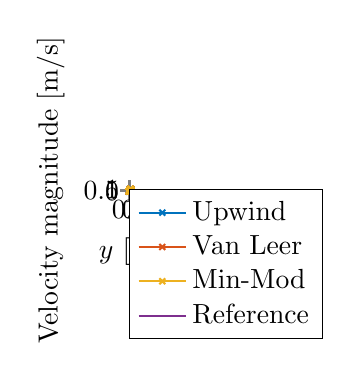
\begin{tikzpicture}

\begin{axis}[%
width=0.951\roughwidth,
height=0.75\roughheight,
at={(0\roughwidth,0\roughheight)},
scale only axis,
xmin=0,
xmax=1.4,
xlabel={$y$ [m]},
ymin=0,
ymax=1.25,
ylabel={Velocity magnitude [m/s]},
axis background/.style={fill=white},
legend style={at={(0.03,0.97)}, anchor=north west, legend cell align=left, align=left}
]

\addplot [color=mycolor1, mark size=1.5pt, mark=x, mark options={solid, mycolor1}, line width=0.75pt]
  table[row sep=crcr]{%
0	0\\
0.01	0.00885222\\
0.03	0.0227802\\
0.05	0.0327807\\
0.07	0.0393192\\
0.09	0.043122\\
0.11	0.0448784\\
0.13	0.0451341\\
0.15	0.0442874\\
0.17	0.0426208\\
0.19	0.0403378\\
0.21	0.037597\\
0.23	0.0345472\\
0.25	0.0313691\\
0.27	0.0283253\\
0.29	0.0258075\\
0.31	0.0243184\\
0.33	0.024277\\
0.35	0.0257093\\
0.37	0.0283224\\
0.39	0.0319839\\
0.41	0.0370173\\
0.43	0.044611\\
0.45	0.0576046\\
0.47	0.0818451\\
0.49	0.128213\\
0.51	0.214615\\
0.53	0.35431\\
0.55	0.509962\\
0.57	0.654372\\
0.59	0.77967\\
0.61	0.885193\\
0.63	0.971543\\
0.65	1.03985\\
0.67	1.0919\\
0.69	1.12994\\
0.71	1.15654\\
0.73	1.17426\\
0.75	1.18543\\
0.77	1.19201\\
0.79	1.19557\\
0.81	1.19723\\
0.83	1.1978\\
0.85	1.19779\\
0.87	1.19754\\
0.89	1.19723\\
0.91	1.19698\\
0.93	1.19685\\
0.95	1.19686\\
0.97	1.19703\\
0.99	1.19736\\
1.01	1.19783\\
1.03	1.19841\\
1.05	1.19906\\
1.07	1.19964\\
1.09	1.19992\\
1.11	1.19953\\
1.13	1.19783\\
1.15	1.19384\\
1.17	1.1861\\
1.19	1.17264\\
1.21	1.15086\\
1.23	1.11762\\
1.25	1.06938\\
1.27	1.00254\\
1.29	0.913831\\
1.31	0.800848\\
1.33	0.662508\\
1.35	0.499366\\
1.37	0.313659\\
1.39	0.109156\\
1.4	0\\
};
\addlegendentry{Upwind}

\addplot [color=mycolor2, mark size=1.5pt, mark=x, mark options={solid, mycolor2}, line width=0.75pt]
  table[row sep=crcr]{%
0	0\\
0.01	0.0122335\\
0.03	0.0324848\\
0.05	0.0480886\\
0.07	0.0588624\\
0.09	0.0654371\\
0.11	0.0686113\\
0.13	0.0688211\\
0.15	0.0669287\\
0.17	0.0627025\\
0.19	0.0563737\\
0.21	0.0484432\\
0.23	0.0398216\\
0.25	0.0319033\\
0.27	0.0265586\\
0.29	0.0256695\\
0.31	0.0288832\\
0.33	0.0340499\\
0.35	0.0396606\\
0.37	0.0450472\\
0.39	0.0499693\\
0.41	0.0545328\\
0.43	0.0595794\\
0.45	0.0677895\\
0.47	0.0859627\\
0.49	0.128135\\
0.51	0.214164\\
0.53	0.35562\\
0.55	0.519342\\
0.57	0.670222\\
0.59	0.798895\\
0.61	0.905422\\
0.63	0.991025\\
0.65	1.05726\\
0.67	1.10635\\
0.69	1.14101\\
0.71	1.16412\\
0.73	1.17855\\
0.75	1.18688\\
0.77	1.19113\\
0.79	1.19289\\
0.81	1.19325\\
0.83	1.1929\\
0.85	1.19227\\
0.87	1.19163\\
0.89	1.19106\\
0.91	1.19067\\
0.93	1.19044\\
0.95	1.19037\\
0.97	1.1905\\
0.99	1.19084\\
1.01	1.19135\\
1.03	1.19204\\
1.05	1.19284\\
1.07	1.19365\\
1.09	1.19427\\
1.11	1.19434\\
1.13	1.19322\\
1.15	1.1899\\
1.17	1.18285\\
1.19	1.16996\\
1.21	1.14851\\
1.23	1.11525\\
1.25	1.06662\\
1.27	0.999152\\
1.29	0.909811\\
1.31	0.796478\\
1.33	0.658286\\
1.35	0.495815\\
1.37	0.311267\\
1.39	0.108298\\
1.4	0\\
};
\addlegendentry{Van Leer}

\addplot [color=mycolor3, mark size=1.5pt, mark=x, mark options={solid, mycolor3}, line width=0.75pt]
  table[row sep=crcr]{%
0	0\\
0.01	0.0113419\\
0.03	0.0297822\\
0.05	0.0438459\\
0.07	0.0535293\\
0.09	0.0594514\\
0.11	0.0623285\\
0.13	0.0627341\\
0.15	0.0613312\\
0.17	0.0581295\\
0.19	0.0533229\\
0.21	0.0472654\\
0.23	0.040544\\
0.25	0.0340756\\
0.27	0.0291588\\
0.29	0.0272168\\
0.31	0.0284915\\
0.33	0.0317763\\
0.35	0.0359173\\
0.37	0.0402998\\
0.39	0.0446982\\
0.41	0.0493064\\
0.43	0.0551453\\
0.45	0.0648297\\
0.47	0.0848545\\
0.49	0.128268\\
0.51	0.214524\\
0.53	0.355773\\
0.55	0.518594\\
0.57	0.668691\\
0.59	0.796856\\
0.61	0.903066\\
0.63	0.988544\\
0.65	1.05485\\
0.67	1.10418\\
0.69	1.13918\\
0.71	1.16273\\
0.73	1.17764\\
0.75	1.1864\\
0.77	1.19104\\
0.79	1.19311\\
0.81	1.19369\\
0.83	1.19352\\
0.85	1.19301\\
0.87	1.19243\\
0.89	1.19193\\
0.91	1.19158\\
0.93	1.19138\\
0.95	1.19133\\
0.97	1.19148\\
0.99	1.19181\\
1.01	1.19232\\
1.03	1.19298\\
1.05	1.19375\\
1.07	1.19452\\
1.09	1.19508\\
1.11	1.19505\\
1.13	1.19379\\
1.15	1.1903\\
1.17	1.18309\\
1.19	1.17005\\
1.21	1.14852\\
1.23	1.11526\\
1.25	1.06673\\
1.27	0.999415\\
1.29	0.910241\\
1.31	0.797042\\
1.33	0.658892\\
1.35	0.496348\\
1.37	0.311635\\
1.39	0.108434\\
1.4	0\\
};
\addlegendentry{Min-Mod}

\addplot [color=mycolor4, line width=0.75pt]
  table[row sep=crcr]{%
0	0\\
0.00166667	0.00162965\\
0.005	0.00480799\\
0.00833333	0.00790634\\
0.0116667	0.0109252\\
0.015	0.013865\\
0.0183333	0.0167258\\
0.0216667	0.019508\\
0.025	0.022212\\
0.0283333	0.0248383\\
0.0316667	0.0273878\\
0.035	0.0298613\\
0.0383333	0.03226\\
0.0416667	0.0345853\\
0.045	0.0368385\\
0.0483333	0.0390211\\
0.0516667	0.0411348\\
0.055	0.0431809\\
0.0583333	0.045161\\
0.0616667	0.0470764\\
0.065	0.0489283\\
0.0683333	0.0507176\\
0.0716667	0.0524452\\
0.075	0.0541115\\
0.0783333	0.055717\\
0.0816667	0.0572619\\
0.085	0.0587457\\
0.0883333	0.0601683\\
0.0916667	0.0615291\\
0.095	0.0628271\\
0.0983333	0.0640617\\
0.101667	0.0652316\\
0.105	0.0663357\\
0.108333	0.0673728\\
0.111667	0.0683414\\
0.115	0.0692403\\
0.118333	0.070068\\
0.121667	0.0708231\\
0.125	0.0715044\\
0.128333	0.0721104\\
0.131667	0.0726401\\
0.135	0.0730923\\
0.138333	0.0734658\\
0.141667	0.0737601\\
0.145	0.0739741\\
0.148333	0.0741073\\
0.151667	0.0741594\\
0.155	0.0741298\\
0.158333	0.0740188\\
0.161667	0.0738262\\
0.165	0.0735523\\
0.168333	0.0731975\\
0.171667	0.0727624\\
0.175	0.0722478\\
0.178333	0.0716544\\
0.181667	0.0709837\\
0.185	0.0702367\\
0.188333	0.0694149\\
0.191667	0.0685199\\
0.195	0.0675533\\
0.198333	0.0665172\\
0.201667	0.0654135\\
0.205	0.0642444\\
0.208333	0.0630124\\
0.211667	0.0617197\\
0.215	0.0603692\\
0.218333	0.0589636\\
0.221667	0.0575058\\
0.225	0.055999\\
0.228333	0.0544466\\
0.231667	0.0528522\\
0.235	0.0512197\\
0.238333	0.0495534\\
0.241667	0.0478579\\
0.245	0.0461384\\
0.248333	0.0444006\\
0.251667	0.042651\\
0.255	0.0408971\\
0.258333	0.0391474\\
0.261667	0.0374118\\
0.265	0.0357016\\
0.268333	0.0340304\\
0.271667	0.032414\\
0.275	0.0308707\\
0.278333	0.0294217\\
0.281667	0.0280915\\
0.285	0.026907\\
0.288333	0.025897\\
0.291667	0.0250911\\
0.295	0.0245166\\
0.298333	0.0241958\\
0.301667	0.0241434\\
0.305	0.024363\\
0.308333	0.0248475\\
0.311667	0.0255795\\
0.315	0.0265348\\
0.318333	0.0276856\\
0.321667	0.0290029\\
0.325	0.0304586\\
0.328333	0.0320267\\
0.331667	0.0336841\\
0.335	0.0354105\\
0.338333	0.0371883\\
0.341667	0.0390024\\
0.345	0.0408399\\
0.348333	0.0426898\\
0.351667	0.0445425\\
0.355	0.04639\\
0.358333	0.048225\\
0.361667	0.0500416\\
0.365	0.0518343\\
0.368333	0.0535986\\
0.371667	0.0553303\\
0.375	0.0570259\\
0.378333	0.0586824\\
0.381667	0.060297\\
0.385	0.0618676\\
0.388333	0.0633923\\
0.391667	0.0648697\\
0.395	0.0662986\\
0.398333	0.0676785\\
0.401667	0.0690093\\
0.405	0.0702916\\
0.408333	0.0715265\\
0.411667	0.072716\\
0.415	0.0738628\\
0.418333	0.0749713\\
0.421667	0.076047\\
0.425	0.0770969\\
0.428333	0.0781306\\
0.431667	0.0791597\\
0.435	0.0801992\\
0.438333	0.0812674\\
0.441667	0.0823869\\
0.445	0.0835853\\
0.448333	0.084896\\
0.451667	0.0863585\\
0.455	0.08802\\
0.458333	0.0899355\\
0.461667	0.0921692\\
0.465	0.0947941\\
0.468333	0.0978929\\
0.471667	0.101558\\
0.475	0.105891\\
0.478333	0.111\\
0.481667	0.117001\\
0.485	0.124015\\
0.488333	0.13216\\
0.491667	0.141554\\
0.495	0.152307\\
0.498333	0.164518\\
0.501667	0.178267\\
0.505	0.193612\\
0.508333	0.210581\\
0.511667	0.229172\\
0.515	0.249346\\
0.518333	0.271026\\
0.521667	0.294097\\
0.525	0.318416\\
0.528333	0.3438\\
0.531667	0.370031\\
0.535	0.396864\\
0.538333	0.42408\\
0.541667	0.451482\\
0.545	0.478885\\
0.548333	0.506133\\
0.551667	0.533085\\
0.555	0.559629\\
0.558333	0.585678\\
0.561667	0.611162\\
0.565	0.636036\\
0.568333	0.660269\\
0.571667	0.683845\\
0.575	0.706758\\
0.578333	0.729008\\
0.581667	0.750601\\
0.585	0.771545\\
0.588333	0.79185\\
0.591667	0.811525\\
0.595	0.83058\\
0.598333	0.849024\\
0.601667	0.866863\\
0.605	0.884107\\
0.608333	0.900759\\
0.611667	0.916826\\
0.615	0.932313\\
0.618333	0.947225\\
0.621667	0.961569\\
0.625	0.975348\\
0.628333	0.988573\\
0.631667	1.00125\\
0.635	1.01338\\
0.638333	1.02498\\
0.641667	1.03605\\
0.645	1.04661\\
0.648333	1.05667\\
0.651667	1.06623\\
0.655	1.07531\\
0.658333	1.08392\\
0.661667	1.09207\\
0.665	1.09978\\
0.668333	1.10705\\
0.671667	1.11391\\
0.675	1.12035\\
0.678333	1.12641\\
0.681667	1.13209\\
0.685	1.1374\\
0.688333	1.14237\\
0.691667	1.147\\
0.695	1.15131\\
0.698333	1.15531\\
0.701667	1.15901\\
0.705	1.16244\\
0.708333	1.1656\\
0.711667	1.16851\\
0.715	1.17118\\
0.718333	1.17363\\
0.721667	1.17586\\
0.725	1.17789\\
0.728333	1.17974\\
0.731667	1.18141\\
0.735	1.18291\\
0.738333	1.18425\\
0.741667	1.18546\\
0.745	1.18653\\
0.748333	1.18747\\
0.751667	1.18831\\
0.755	1.18903\\
0.758333	1.18966\\
0.761667	1.1902\\
0.765	1.19066\\
0.768333	1.19104\\
0.771667	1.19135\\
0.775	1.19161\\
0.778333	1.19181\\
0.781667	1.19195\\
0.785	1.19206\\
0.788333	1.19212\\
0.791667	1.19214\\
0.795	1.19214\\
0.798333	1.19211\\
0.801667	1.19205\\
0.805	1.19197\\
0.808333	1.19188\\
0.811667	1.19177\\
0.815	1.19164\\
0.818333	1.19151\\
0.821667	1.19136\\
0.825	1.19121\\
0.828333	1.19106\\
0.831667	1.1909\\
0.835	1.19073\\
0.838333	1.19057\\
0.841667	1.19041\\
0.845	1.19025\\
0.848333	1.19009\\
0.851667	1.18993\\
0.855	1.18977\\
0.858333	1.18962\\
0.861667	1.18947\\
0.865	1.18933\\
0.868333	1.18919\\
0.871667	1.18906\\
0.875	1.18893\\
0.878333	1.18881\\
0.881667	1.18869\\
0.885	1.18858\\
0.888333	1.18847\\
0.891667	1.18838\\
0.895	1.18828\\
0.898333	1.1882\\
0.901667	1.18812\\
0.905	1.18804\\
0.908333	1.18797\\
0.911667	1.18791\\
0.915	1.18786\\
0.918333	1.18781\\
0.921667	1.18776\\
0.925	1.18773\\
0.928333	1.1877\\
0.931667	1.18767\\
0.935	1.18765\\
0.938333	1.18764\\
0.941667	1.18763\\
0.945	1.18763\\
0.948333	1.18764\\
0.951667	1.18765\\
0.955	1.18767\\
0.958333	1.18769\\
0.961667	1.18772\\
0.965	1.18776\\
0.968333	1.1878\\
0.971667	1.18785\\
0.975	1.1879\\
0.978333	1.18797\\
0.981667	1.18803\\
0.985	1.18811\\
0.988333	1.18818\\
0.991667	1.18827\\
0.995	1.18836\\
0.998333	1.18846\\
1.00167	1.18856\\
1.005	1.18867\\
1.00833	1.18879\\
1.01167	1.18891\\
1.015	1.18904\\
1.01833	1.18917\\
1.02167	1.18931\\
1.025	1.18946\\
1.02833	1.18961\\
1.03167	1.18977\\
1.035	1.18993\\
1.03833	1.1901\\
1.04167	1.19027\\
1.045	1.19045\\
1.04833	1.19063\\
1.05167	1.19081\\
1.055	1.191\\
1.05833	1.19119\\
1.06167	1.19139\\
1.065	1.19158\\
1.06833	1.19177\\
1.07167	1.19197\\
1.075	1.19216\\
1.07833	1.19235\\
1.08167	1.19253\\
1.085	1.19271\\
1.08833	1.19288\\
1.09167	1.19305\\
1.095	1.1932\\
1.09833	1.19333\\
1.10167	1.19345\\
1.105	1.19355\\
1.10833	1.19362\\
1.11167	1.19367\\
1.115	1.19369\\
1.11833	1.19368\\
1.12167	1.19363\\
1.125	1.19353\\
1.12833	1.19338\\
1.13167	1.19319\\
1.135	1.19293\\
1.13833	1.1926\\
1.14167	1.1922\\
1.145	1.19172\\
1.14833	1.19115\\
1.15167	1.19049\\
1.155	1.18971\\
1.15833	1.18883\\
1.16167	1.18782\\
1.165	1.18667\\
1.16833	1.18538\\
1.17167	1.18393\\
1.175	1.18231\\
1.17833	1.18051\\
1.18167	1.17852\\
1.185	1.17632\\
1.18833	1.17389\\
1.19167	1.17123\\
1.195	1.16832\\
1.19833	1.16515\\
1.20167	1.1617\\
1.205	1.15794\\
1.20833	1.15388\\
1.21167	1.14949\\
1.215	1.14475\\
1.21833	1.13965\\
1.22167	1.13417\\
1.225	1.12829\\
1.22833	1.12201\\
1.23167	1.11529\\
1.235	1.10812\\
1.23833	1.1005\\
1.24167	1.09239\\
1.245	1.08378\\
1.24833	1.07466\\
1.25167	1.06502\\
1.255	1.05483\\
1.25833	1.04408\\
1.26167	1.03276\\
1.265	1.02085\\
1.26833	1.00835\\
1.27167	0.995228\\
1.275	0.981485\\
1.27833	0.967108\\
1.28167	0.952085\\
1.285	0.936409\\
1.28833	0.92007\\
1.29167	0.903062\\
1.295	0.885377\\
1.29833	0.867011\\
1.30167	0.847959\\
1.305	0.828218\\
1.30833	0.807786\\
1.31167	0.786662\\
1.315	0.764846\\
1.31833	0.742339\\
1.32167	0.719144\\
1.325	0.695264\\
1.32833	0.670704\\
1.33167	0.645471\\
1.335	0.619571\\
1.33833	0.593012\\
1.34167	0.565805\\
1.345	0.537959\\
1.34833	0.509487\\
1.35167	0.480401\\
1.355	0.450714\\
1.35833	0.420443\\
1.36167	0.389601\\
1.365	0.358207\\
1.36833	0.326277\\
1.37167	0.29383\\
1.375	0.260885\\
1.37833	0.227463\\
1.38167	0.193583\\
1.385	0.159268\\
1.38833	0.124538\\
1.39167	0.0894149\\
1.395	0.0539223\\
1.39833	0.0180823\\
1.4	0\\
};
\addlegendentry{Reference}
\addplot [color=black, dashed, line width=0.75pt]
  table[row sep=crcr]{%
0.5	0\\
0.5 1.25\\
};
\end{axis}
\end{tikzpicture}%
	\caption[Profile of the magnitude of the velocity in the rough channel with 
	deep cavities at $Re=\num{2.8e3}$]{Profile of the magnitude of the velocity 
		$[\si{m/s}]$ in the rough channel with deep cavities along the 
		cross-section 
		$x=\SI{8.75}{m}$, at $t=T$. $Re=\num{2.8e3}$. The region on 
		the 
		left of the dashed line is inside the cavity.}
	\label{fig:linecompdeep}
\end{figure}
\begin{table}
	\centering
	\[
	\begin{array}{ccc}
	\toprule
	\text{Upwind} & \text{Van Leer} & \text{Van Alabada}\\
	\midrule
	\num{3.180e-4} & \num{5.862e-5} & \num{6.900e-5}\\
	\midrule
	\text{Min-Mod} & \text{Superbee} & \text{MC Limiter} \\
	\midrule
	\num{8.579e-5} & \num{7.883e-5} & \num{5.584e-5}\\
	\bottomrule
	\end{array}
	\]
	\caption[$L^2(\Omega)$ norm of the errors for the profile of the magnitude 
	of the 
	velocity in 
	the rough channel with deep cavities]{$L^2(\Omega)$ norm of the errors for 
	the profile 
	of the 
	magnitude of the velocity along the cross-section at $x=\SI{8.75}{m}$ and 
	$t=T$ in the rough channel with deep cavities. $Re = \num{2.8e3}$.}
	\label{tab:errdeep}
\end{table}
%
\section{RANS test: backward facing step} \label{sec:bfs}
The backward facing step is a widely-used test configuration, in which a 
turbulent flow in a channel incurs separation because of a sudden enlargement 
in the flow domain. We can see that in Figure~\ref{fig:bfsarrows} there are a 
big recirculation after the step, a smaller eddy near the corner and a very 
small 
eddy precisely at the corner. We want to use this problem in order to test the 
results that we obtain using the TVD method, with the Van Leer flux limiter 
\eqref{eq:vl}, and the $k\text{-}\omega$ turbulence model, comparing them with 
the numerical results from \cite{web:nasa}, computed using the NASA CFL3D code, 
and the experimental results from \cite{bfs:driver}.

In the domain $\Omega$, depicted in Figure~\ref{fig:bfsdomain}, with a step height $H=\SI{1}{m}$, we solve the RANS equations \eqref{eq:ransmass}-\eqref{eq:ransmom}-\eqref{eq:komegak}-\eqref{eq:komegaomega}, imposing inflow boundary conditions on the left boundary $\Gamma_\text{in}$
\begin{equation}
	\mathbf{v} = \mathbf{v}_\text{in} = [u_\text{in}, 0]^\mathrm{T}, \quad u_\text{in} = \SI{44.2}{m/s},
\end{equation} no-slip boundary conditions on the lower and upper boundaries $\Gamma_w$ and outflow boundary conditions on the right boundary $\Gamma_\text{out}$, fixing the value of pressure
\begin{equation}
	p = p_\text{ext} = \SI{1.1e5}{\pascal}.
\end{equation}
\begin{figure}
	\centering
	\includegraphics[width=\textwidth]{bfs_domain_axis.pdf}
	\caption[Domain of the backward facing step test]{Domain $\Omega$ of the backward facing step test. For convenience, we set the origin of the $x$-axis in correspondence of the step and the origin of the $y$-axis at the bottom of the channel.}
	\label{fig:bfsdomain}
\end{figure}
The density is $\varrho = \SI{1}{kg/m^3}$ and the viscosity is $\nu=\SI{1.228e-3}{m^2/s}$, so that, in order to match \cite{web:nasa}, the Reynolds number based on the step height results
\begin{equation}
	Re_H = \frac{u_\text{in}H}{\nu} \simeq \num{3.6e4}.
\end{equation}

The domain sizes are chosen according to \cite{web:nasa}, with the only 
exception of the channel length before the step. In fact, in \cite{web:nasa}, a 
small portion of the horizontal boundary near $\Gamma_\text{in}$ uses symmetry 
boundary conditions, but we simplify the model employing no-slip boundary 
conditions on the whole horizontal boundaries. As a consequence, we shorten the 
channel length in order to match the profile of the $u$ 
component of the velocity along the cross-section at the position $x/H=-4$ as closely as possible, 
with a boundary layer thickness of approximately $1.5H$ (see 
Figure~\ref{fig:bfscomp}).

According to \cite{web:nasa}, CFL3D is a code for compressible fluids, but it was used at ``essentially incompressible'' conditions, such that the influence of compressibility should be very small. Moreover it is reported that, running unsteady simulations, the solution settles down and becomes reasonably steady (quasi-steady); in \cite{bfs:cfl3d} it is explained that a second order implicit method for the advancement in time is used.

Thus, we employ the BDF2 method for non-constant time-steps \eqref{eq:bdf2gen}, starting from $\Delta t = \SI{e-5}{s}$ and simulating until $T = \SI{30}{s}$. It can be observed that, after approximately $t=\SI{20}{s}$, the solution stabilizes at a steady state. As initial conditions we set
\begin{equation}
p=p_\text{ext} \quad \forall \mathbf{x} \in \Omega, \quad \mathbf{v} = [u_\text{init},0]^\mathrm{T} \quad u_\text{init} = \begin{cases}
u_\text{in} \quad&\text{if $x\leq 0$}\\
\frac{8}{9}u_\text{in} \quad&\text{if $x>0$}
\end{cases}
\end{equation}
The factor $8/9$ ensures that the flow rate at $\Gamma_\text{in}$ and at $\Gamma_\text{out}$ is the same. For $k$ and $\omega$ we set in the whole domain the values estimated with \eqref{eq:koic}.

According to \cite{web:nasa}, a key indicator for the reliability of a 
simulation is the prediction of the \emph{reattachment length} $l_\text{rea}$, 
i.e. the distance after the step at which the recirculation finishes and thus 
the $u$ component of the velocity at the bottom of the channel becomes 
positive. We analyse this length computing the \emph{friction coefficient} 
$C_f$, that is a non-dimensional form of the stress at the wall, which is 
defined by:
\begin{equation}
C_f = \frac{\tau_w}{\frac{1}{2}\varrho U_\text{ref}^2}, \quad \tau_w = \mu \frac{\partial u}{\partial y} \Big|_{y=0}.
\end{equation}
$U_\text{ref}$ is the $u$ component of the velocity at the centre of the channel at $x/H=-4$. In our case when $C_f<0$ the flow is recirculating, then, at $x=l_{rea}$, $C_f$ becomes positive. The numerical results from \cite{web:nasa} predict $l_\text{rea}/H \simeq 6.8$, while the experimental results from \cite{bfs:driver} predict $l_\text{rea}/H = 6.26 \pm 0.10$, as it can be seen in Figure~\ref{fig:bfscf}.

Performing a sensitivity analysis in order to choose a suitable grid, we observe that:
\begin{itemize}
	\item with a coarse mesh the reattachment length decreases, in particular a refinement of the smallest cell in the $y$-direction is effective.
	\item too stretched cells increase the number of Newton iteration needed to get the convergence of the problem.
	\item the cells in the portion of the channel after the step can be coarsened in the $x$-direction without a great influence on the solution.
	\item too refined cells in the $y$-direction in the area with the 
	recirculation do not improve the solution in a relevant way.
\end{itemize}
So, in the following analysis, we choose a grid made of $\num{119x70}$ cells, employing gradings up to 1.25 in order to have small cells near the walls, as it is required by the $k\text{-}\omega$ model. In Figure~\ref{fig:bfsgrid} we can see the grid in the region around the step.

\begin{figure} %mettere in paraview frecce 2d
	\centering
	\includegraphics[width=\textwidth]{bfs_glimphs2.png}
	\caption[Velocity field after the backward facing step]{Velocity field $[\si{m/s}]$ after the backward facing step at $t=T$. $Re_H=\num{3.6e4}$. The arrows are not scaled.}
	\label{fig:bfsarrows}
\end{figure}
%nuova immagine:
\begin{figure}
	\centering
	\includegraphics[width=0.8\textwidth]{bfs_grid.png}
	\caption[Velocity field and grid around the backward facing step]{Velocity field $[\si{m/s}]$ and grid around the backward facing step at $t=T$. $Re_H=\num{3.6e4}$. The arrows are not scaled.}
	\label{fig:bfsgrid}
\end{figure}
\begin{figure}[t]
	\centering
	\input{../img/bfs_fin_cf_report}
	\caption[Friction coefficient in the backward facing step test]{Friction coefficient at the bottom of the channel after the backward facing step at $t=T$. The reattachment length is the distance at which it becomes positive after its global minimum.}
	\label{fig:bfscf}
\end{figure}

Regarding the reattachment length, we obtain a good agreement with the 
CFL3D code; looking at Figure~\ref{fig:bfscf}, with the Van Leer flux 
limiter we predict $l_\text{rea} /H \simeq 6.67$. Moreover, in the whole 
recirculating region, the two patterns are very similar, also compared to the 
experimental data from \cite{bfs:driver}. Using the first order upwind method, 
instead, we compute $l_\text{rea} /H \simeq 6.02$, so approximately a 10\% 
underestimation occurs. From the profile, it seems that the whole recirculation 
is slightly smaller. Looking at the value near the end of the channel, instead, 
both the Van Leer and the upwind show a lower value with respect to the CFL3D 
code. Comparing in Figure~\ref{fig:bfscomp} the profiles of the $u$ component 
of the velocity along some cross-sections downstream with respect to the step, 
we obtain, similarly, a good agreement between the Van Leer results and those 
from the CFL3D code, while the results from the upwind method present a small 
shift, in particular in the cases $x/H=4$ and $x/H=10$. Along the cross-section 
at $x/H=1$, the velocity at the wall is positive for the Van Leer and the 
CFL3D, since we are in correspondence of the corner eddy. For the upwind 
method, instead, the velocity is negative, as we are already in the bigger eddy 
because the whole pattern is shifted.
\begin{figure}
	\centering
	\subfloat[$x/H=-4$]{\input{../img/bfs_fin_vel0_report}}
	\subfloat[$x/H=1$]{% This file was created by matlab2tikz.
%
\definecolor{mycolor4}{rgb}{0.00000,0.44700,0.74100}%
\definecolor{mycolor3}{rgb}{0.85000,0.32500,0.09800}%
\definecolor{mycolor2}{rgb}{0.92900,0.69400,0.12500}%
\definecolor{mycolor1}{rgb}{0.49400,0.18400,0.55600}%
%
\begin{tikzpicture}

\begin{axis}[%
width=0.958\bfshalfwidth,
height=0.75\bfsheight,
at={(0\bfshalfwidth,0\bfsheight)},
scale only axis,
xmin=-0.2,
xmax=1.2,
xlabel={$u/U_\text{ref}$},
ymin=0,
ymax=2,
ytick distance=1,
ylabel style={rotate=-90},
ylabel={$\dfrac{y}{H}$},
axis background/.style={fill=white},
legend style={at={(0.03,0.97)}, anchor=north west, legend cell align=left, align=left, font=\footnotesize, fill=none}
]
\addplot [color=mycolor1, line width=0.75pt]
  table[row sep=crcr]{%
0	0\\
0.0001201796986	0.0001500749349\\
0.0002449547756	0.0003087310179\\
0.0003762734123	0.0004765522899\\
0.0005145065952	0.0006541581242\\
0.0006600376801	0.0008422057144\\
0.000813261373	0.001041392214\\
0.0009745839634	0.00125245715\\
0.001144421869	0.001476185862\\
0.001323200529	0.001713411068\\
0.001511353068	0.001965016825\\
0.001709318836	0.002231941791\\
0.001917539747	0.002515181201\\
0.00213646004	0.002815792104\\
0.002366520697	0.003134895815\\
0.002608157694	0.003473682096\\
0.002861796878	0.003833413823\\
0.003127847333	0.004215430468\\
0.003406698816	0.004621152766\\
0.003698710818	0.005052087829\\
0.004004209302	0.005509833805\\
0.0043234732	0.005996085238\\
0.004656726494	0.006512639113\\
0.005004127044	0.007061398588\\
0.005365749821	0.007644380908\\
0.005741576198	0.008263722993\\
0.006131470203	0.008921687491\\
0.00653516734	0.009620669298\\
0.006952241063	0.0103632044\\
0.007382081822	0.01115197316\\
0.007823864929	0.0119898105\\
0.008276509121	0.0128797153\\
0.008738632314	0.01382485218\\
0.00920849666	0.0148285646\\
0.009683942422	0.01589438133\\
0.01016229764	0.01702602394\\
0.01064029057	0.0182274133\\
0.01111392584	0.01950268447\\
0.01157834847	0.02085618302\\
0.01202771906	0.02229248732\\
0.01245508343	0.023816403\\
0.01285232976	0.02543297783\\
0.01321025286	0.02714750916\\
0.01351886801	0.02896554396\\
0.013767967	0.03089288995\\
0.01394800935	0.03293561935\\
0.01405109838	0.03510007635\\
0.01407186221	0.03739286959\\
0.01400783751	0.03982088342\\
0.01385922916	0.04239127785\\
0.01362809725	0.04511147365\\
0.01331724878	0.04798916727\\
0.01292915177	0.05103230849\\
0.01246509328	0.05424910039\\
0.01192465518	0.0576479882\\
0.01130547561	0.0612376295\\
0.01060321368	0.06502689421\\
0.009811639786	0.06902483106\\
0.008922834881	0.07324063778\\
0.007927447557	0.07768364996\\
0.006814987864	0.08236327022\\
0.005573913921	0.08728893846\\
0.004191290587	0.09247011691\\
0.00265187677	0.09791619331\\
0.0009385751327	0.1036364213\\
-0.000963122875	0.1096399054\\
-0.003060560208	0.1159354597\\
-0.005352776032	0.1225315928\\
-0.00783053413	0.1294363886\\
-0.01047685929	0.1366574168\\
-0.01326751336	0.1442016512\\
-0.01617241837	0.1520753801\\
-0.01915765554	0.1602840871\\
-0.02218494006	0.1688323319\\
-0.02521179989	0.1777237058\\
-0.02819362469	0.1869606376\\
-0.03108495846	0.1965443641\\
-0.0338409096	0.2064747959\\
-0.03641942516	0.2167504281\\
-0.03878329694	0.2273682207\\
-0.04090159386	0.2383235991\\
-0.04275062308	0.249610275\\
-0.04431445152	0.2612203062\\
-0.04558489099	0.2731439471\\
-0.04656100646	0.2853696942\\
-0.04724829271	0.2978843451\\
-0.04765757173	0.3106728196\\
-0.0478037782	0.323718369\\
-0.04770476744	0.3370026648\\
-0.04738013446	0.3505057096\\
-0.04685027897	0.3642061055\\
-0.04613560811	0.3780810535\\
-0.04525596648	0.3921067119\\
-0.04423021153	0.4062580764\\
-0.04307601228	0.4205094278\\
-0.04180970788	0.4348344207\\
-0.04044631869	0.4492062032\\
-0.0389995873	0.4635978639\\
-0.03748202324	0.4779824615\\
-0.0359050557	0.492333293\\
-0.03427907825	0.5066241622\\
-0.03261359036	0.520829618\\
-0.03091723472	0.5349249244\\
-0.02919791639	0.5488865972\\
-0.02746286616	0.5626922846\\
-0.02571871504	0.5763211846\\
-0.02397154085	0.5897538066\\
-0.02222687751	0.6029724479\\
-0.02048963681	0.615961194\\
-0.01876389422	0.6287056804\\
-0.01705254801	0.6411936283\\
-0.01535683684	0.6534144878\\
-0.01367580146	0.6653595567\\
-0.01200577244	0.6770219207\\
-0.01033997722	0.6883966327\\
-0.008668510243	0.6994803548\\
-0.006978513673	0.7102713585\\
-0.005254388321	0.7207696438\\
-0.003478127997	0.7309766412\\
-0.001629842911	0.7408953309\\
0.0003117911983	0.7505297661\\
0.002369261347	0.7598854303\\
0.004565290641	0.7689688206\\
0.0069238469	0.7777875066\\
0.009470882826	0.7863498926\\
0.01223075204	0.794665277\\
0.0152295148	0.8027436137\\
0.01849941164	0.8105954528\\
0.02206458524	0.8182319403\\
0.02592881024	0.8256042004\\
0.0300907474	0.8326897025\\
0.03455769271	0.8394981027\\
0.03933769464	0.8460389972\\
0.04443381354	0.8523222208\\
0.04984596372	0.8583575487\\
0.0555716306	0.8641546965\\
0.06160631776	0.8697232008\\
0.06794383377	0.8750725389\\
0.07457635552	0.8802121878\\
0.08149473369	0.8851511478\\
0.08868864924	0.8898984194\\
0.09614694118	0.8944627047\\
0.1038577408	0.8988524675\\
0.1118080467	0.9030758739\\
0.1199838817	0.9071409106\\
0.1283706129	0.9110552073\\
0.1369528472	0.9148262739\\
0.1457143724	0.918461144\\
0.154637903	0.9219666123\\
0.1637056172	0.9253494143\\
0.1728995144	0.9286156893\\
0.1822014153	0.9317715764\\
0.1915930361	0.9348228574\\
0.2010559142	0.9377749562\\
0.2105716169	0.9406331778\\
0.2201218307	0.9434025884\\
0.2296884507	0.9460878968\\
0.2392538488	0.9486937523\\
0.2488009483	0.9512243867\\
0.2583136857	0.953684032\\
0.2677771151	0.9560765624\\
0.277177304	0.9584057331\\
0.286501348	0.9606750607\\
0.295737803	0.9628879428\\
0.3048765957	0.9650474787\\
0.3139089346	0.9671568274\\
0.3228273988	0.9692187309\\
0.3316257298	0.9712360501\\
0.3402987123	0.9732112885\\
0.3488423824	0.9751468897\\
0.3572541475	0.9770451784\\
0.3655327559	0.9789084196\\
0.3736785948	0.9807386398\\
0.3816936612	0.982537806\\
0.3895806074	0.9843078852\\
0.3973421156	0.9860506058\\
0.4049801826	0.9877676368\\
0.4124955237	0.9894605279\\
0.4198876917	0.9911309481\\
0.4271561205	0.9927802086\\
0.4343010783	0.9944097996\\
0.4413248301	0.9960208535\\
0.4482325017	0.9976147413\\
0.4550318718	0.9991925955\\
0.4617332518	1.000755548\\
0.4683483839	1.002304673\\
0.4748881757	1.003840923\\
0.4813614488	1.005365252\\
0.4877739847	1.006878734\\
0.4941294789	1.008381963\\
0.5004304647	1.009876132\\
0.506678462	1.011361718\\
0.5128827095	1.012839675\\
0.5190678239	1.014318705\\
0.5252566934	1.015807629\\
0.5314542055	1.017307401\\
0.537656188	1.018818736\\
0.5438578725	1.02034235\\
0.5500535369	1.021879435\\
0.5562369227	1.023430705\\
0.5624008775	1.024997234\\
0.5685377121	1.026580215\\
0.5746390224	1.02818048\\
0.5806956887	1.029799461\\
0.5866978765	1.031438231\\
0.5926355124	1.033098221\\
0.5984978676	1.034780741\\
0.6042742729	1.036487222\\
0.6099542379	1.038219213\\
0.6155272126	1.039978385\\
0.6209841967	1.041766405\\
0.6263165474	1.043585062\\
0.6315172315	1.045436382\\
0.6365810037	1.047322392\\
0.6415042877	1.049245119\\
0.6462858915	1.051206946\\
0.6509258747	1.053210378\\
0.6554266214	1.055257797\\
0.6597916484	1.057352066\\
0.6640262008	1.059496045\\
0.6681365371	1.061692715\\
0.6721298695	1.063945413\\
0.6760143042	1.066257596\\
0.6797982454	1.068632841\\
0.6834904552	1.071074963\\
0.6870999336	1.073588252\\
0.6906355023	1.076176882\\
0.6941058636	1.078845739\\
0.6975193024	1.081599474\\
0.7008841038	1.08444345\\
0.7042078376	1.08738327\\
0.707497716	1.090424657\\
0.7107604742	1.093573928\\
0.7140023708	1.096837759\\
0.7172290087	1.100223184\\
0.7204455137	1.103737593\\
0.723656714	1.107388973\\
0.7268668413	1.111185789\\
0.7300795913	1.115136862\\
0.7332985401	1.119251847\\
0.7365266085	1.123540759\\
0.739766717	1.128014207\\
0.743021071	1.132683516\\
0.7462921739	1.137560844\\
0.7495819926	1.142658949\\
0.7528924346	1.14799118\\
0.7562254667	1.153571963\\
0.7595828772	1.159416676\\
0.7629670501	1.165541291\\
0.7663809061	1.171962857\\
0.7698261142	1.178699493\\
0.7733042836	1.185770392\\
0.7768170238	1.19319582\\
0.7803665996	1.200997233\\
0.7839553952	1.209197283\\
0.7875868678	1.217820168\\
0.791264832	1.226891041\\
0.794998765	1.236445308\\
0.7988060117	1.246588945\\
0.8026977181	1.257356644\\
0.8066765666	1.268784761\\
0.8107457757	1.280911565\\
0.814909339	1.293777347\\
0.8191700578	1.307424188\\
0.8235276937	1.321896553\\
0.8279781342	1.337240696\\
0.8325152397	1.353505373\\
0.83713305	1.37074101\\
0.8418268561	1.389000773\\
0.8465935588	1.408339858\\
0.8514311314	1.428815722\\
0.8563382626	1.45048821\\
0.8613141775	1.473419428\\
0.866358161	1.497673512\\
0.8714694977	1.523316979\\
0.8766474724	1.550418496\\
0.8818910122	1.579048634\\
0.8871990442	1.60927999\\
0.8925704956	1.641186953\\
0.898003757	1.674845338\\
0.9034971595	1.710332632\\
0.9090492129	1.747727394\\
0.9146580696	1.787108898\\
0.9203218818	1.828557253\\
0.9260393381	1.872152448\\
0.931809783	1.917974591\\
0.9376343489	1.966102839\\
0.9435166121	2.016615391\\
0.949464798	2.069588423\\
0.9554941058	2.125096083\\
0.9616293311	2.183209419\\
0.9679220319	2.243995428\\
0.9744608402	2.30751729\\
0.9812601209	2.373832703\\
0.9880837798	2.442992687\\
0.9944391251	2.515042067\\
0.9997528195	2.590017557\\
1.003531337	2.667947292\\
1.005473375	2.74884963\\
1.005714655	2.832732677\\
1.004964709	2.919592857\\
1.004065752	3.009414673\\
1.003312945	3.102169275\\
1.002584815	3.197814703\\
1.001843572	3.296294689\\
1.001107931	3.39753747\\
1.00037539	3.501456976\\
0.9996489286	3.607951164\\
0.9989302754	3.716902971\\
0.9982210994	3.828179598\\
0.9975233078	3.941633224\\
0.9968384504	4.05710125\\
0.9961681962	4.174407482\\
0.9955137372	4.293362617\\
0.9948765039	4.413764\\
0.9942575097	4.535399437\\
0.993657887	4.658046722\\
0.9930784106	4.781475544\\
0.9925195575	4.90544939\\
0.9919822216	5.029727459\\
0.9914666414	5.154065132\\
0.9909728169	5.278218746\\
0.9905010462	5.40194416\\
0.9900514483	5.525001526\\
0.9896235466	5.647155285\\
0.9892175198	5.768176556\\
0.9888327122	5.887844563\\
0.988468945	6.005949974\\
0.9881252646	6.122292519\\
0.9878017902	6.236685753\\
0.9874976873	6.348957539\\
0.9872118831	6.458948612\\
0.9869410992	6.566515446\\
0.9866840839	6.671530724\\
0.9864527583	6.773881435\\
0.9862836599	6.873472214\\
0.9861841798	6.970221519\\
0.9859330058	7.06406498\\
0.9848447442	7.154951572\\
0.9819204807	7.242846489\\
0.9765970707	7.327727318\\
0.9693519473	7.409585476\\
0.9611264467	7.488424301\\
0.952534914	7.564259052\\
0.9439306259	7.637114048\\
0.9355815053	7.707024574\\
0.9276411533	7.774034023\\
0.9201068878	7.83819294\\
0.9128187895	7.899559498\\
0.9055902958	7.958196163\\
0.8983525634	8.0141716\\
0.891115427	8.067558289\\
0.8838909268	8.118432045\\
0.8766872883	8.166871071\\
0.869509697	8.212956429\\
0.8623616695	8.25676918\\
0.8552448153	8.298392296\\
0.8481599689	8.337908745\\
0.8411070108	8.375400543\\
0.8340851665	8.410949707\\
0.827093184	8.444638252\\
0.8201296926	8.476546288\\
0.8131930828	8.506752014\\
0.8062813878	8.53533268\\
0.7993926406	8.562361717\\
0.7925251722	8.587914467\\
0.7856765985	8.612060547\\
0.7788453698	8.634868622\\
0.7720292807	8.656404495\\
0.7652266026	8.676732063\\
0.758435607	8.695914268\\
0.7516543269	8.714008331\\
0.7448812127	8.731071472\\
0.7381145954	8.747159004\\
0.7313529253	8.762321472\\
0.7245946527	8.776609421\\
0.7178381681	8.79006958\\
0.7110818624	8.802747726\\
0.7043243647	8.814686775\\
0.6975641251	8.825927734\\
0.6907993555	8.836508751\\
0.6840286255	8.846467972\\
0.6772500873	8.855840683\\
0.6704618931	8.864658356\\
0.6636622548	8.872954369\\
0.6568490267	8.880758286\\
0.6500199437	8.888097763\\
0.6431726217	8.894999504\\
0.6363046169	8.901489258\\
0.6294131279	8.90759182\\
0.6224950552	8.913328171\\
0.6155471802	8.918721199\\
0.6085661054	8.923790932\\
0.6015481949	8.928555489\\
0.5944893956	8.93303299\\
0.5873852968	8.937240601\\
0.5802314878	8.941195488\\
0.5730227828	8.944911003\\
0.565753758	8.948401451\\
0.5584187508	8.951682091\\
0.5510112643	8.954763412\\
0.5435245633	8.957657814\\
0.5359511375	8.960377693\\
0.5282828808	8.962932587\\
0.5205109715	8.965332031\\
0.5126258731	8.967585564\\
0.504617095	8.969702721\\
0.4964732528	8.971691132\\
0.48818174	8.973558426\\
0.4797289073	8.975313187\\
0.4710996747	8.976960182\\
0.4622774124	8.978507042\\
0.4532440007	8.979959488\\
0.4439793527	8.981324196\\
0.434461236	8.98260498\\
0.424665451	8.983808517\\
0.4145650268	8.984937668\\
0.4041306078	8.985999107\\
0.3933300376	8.986994743\\
0.3821282983	8.987930298\\
0.3704878986	8.988808632\\
0.358369261	8.98963356\\
0.3457316458	8.990407944\\
0.3325349689	8.991134644\\
0.3187426925	8.991817474\\
0.3043266535	8.992458344\\
0.2892735004	8.993061066\\
0.2735939324	8.993625641\\
0.25733307	8.994156837\\
0.2405813336	8.994654655\\
0.2234797478	8.99512291\\
0.2062170506	8.9955616\\
0.1890131831	8.995974541\\
0.1720929593	8.996361732\\
0.1556569785	8.996725082\\
0.1398601979	8.997066498\\
0.1248037815	8.997386932\\
0.1105391756	8.99768734\\
0.09707921743	8.997969627\\
0.08441054076	8.998234749\\
0.07250424474	8.998484612\\
0.06132347509	8.998718262\\
0.05082828552	8.998937607\\
0.04097843543	8.9991436\\
0.03173483163	8.999337196\\
0.02306023054	8.999519348\\
0.01491948031	8.999689102\\
0.007279536221	8.999849319\\
0	9\\
};
\addlegendentry{CFL3D}

\addplot [color=mycolor2, draw=none, mark=x, mark options={solid, mycolor2}, only marks]
  table[row sep=crcr]{%
-0.008	0.1\\
-0.017	0.15\\
-0.027	0.2\\
-0.035	0.3\\
-0.035	0.4\\
-0.035	0.5\\
-0.027	0.6\\
-0.005	0.7\\
0.081	0.8\\
0.292	0.9\\
0.519	1\\
0.704	1.1\\
0.74	1.15\\
0.762	1.2\\
0.793	1.3\\
0.827	1.4\\
0.851	1.5\\
0.891	1.7\\
0.942	2\\
0.99	2.4\\
1.009	2.8\\
1.003	3.2\\
1.002	3.6\\
1	4\\
0.997	5\\
0.994	6\\
0.993	7.5\\
0.919	8.2\\
};
\addlegendentry{Experiment}

\addplot [color=mycolor3, line width=0.75pt]
  table[row sep=crcr]{%
0	0\\
0.00912534743726842	0.009\\
0.00909328784414237	0.018\\
0.0024880687309673	0.027\\
-0.00577625575668998	0.036\\
-0.0148990529990506	0.045\\
-0.0229067507302344	0.054\\
-0.0308380711954414	0.063\\
-0.0367688816216668	0.072\\
-0.0426996920478922	0.081\\
-0.0472199660974089	0.09\\
-0.0510786895855612	0.099\\
-0.0549374130737135	0.108\\
-0.0572450180120909	0.117\\
-0.0593376779511005	0.126\\
-0.0614303378901102	0.135\\
-0.0628387312458881	0.144\\
-0.0636037897182142	0.153\\
-0.0643690624926334	0.162\\
-0.0651343352670525	0.171\\
-0.0654656463029674	0.18\\
-0.0653272071508322	0.189\\
-0.0651887679986971	0.198\\
-0.0650505431486549	0.207\\
-0.0649121039965197	0.216\\
-0.0644138516300889	0.225\\
-0.0637109407647584	0.234\\
-0.0630082442015211	0.243\\
-0.0623055476382838	0.252\\
-0.0616026367729534	0.261\\
-0.060899940209716	0.27\\
-0.0599038640810405	0.279\\
-0.0588462832516485	0.288\\
-0.0577887024222566	0.297\\
-0.0567313358949577	0.306\\
-0.0556737550655657	0.315\\
-0.0546161742361738	0.324\\
-0.0535585934067818	0.333\\
-0.052293353849187	0.342\\
-0.0509923258420465	0.351\\
-0.049691297834906	0.36\\
-0.0483902698277654	0.369\\
-0.0470892418206249	0.378\\
-0.0457882138134843	0.387\\
-0.0444869715042507	0.396\\
-0.0431859434971101	0.405\\
-0.041837554727397	0.414\\
-0.0404390192679012	0.423\\
-0.0390404838084054	0.432\\
-0.0376419483489095	0.441\\
-0.0362434128894137	0.45\\
-0.0348450917320109	0.459\\
-0.0334465562725151	0.468\\
-0.0320480208130193	0.477\\
-0.0306494853535234	0.486\\
-0.0292509498940276	0.495\\
-0.0277881238066052	0.504\\
-0.0262453630384608	0.513\\
-0.0247023879682233	0.522\\
-0.0231596272000789	0.531\\
-0.0216166521298413	0.54\\
-0.0200738699314876	0.549\\
-0.0185310020122967	0.558\\
-0.0169881340931057	0.567\\
-0.015445287604124	0.576\\
-0.0139024196849331	0.585\\
-0.0122419213468458	0.594\\
-0.0104072811279148	0.603\\
-0.00857266233919307	0.612\\
-0.00673802212026205	0.621\\
-0.00490338190133103	0.63\\
-0.00306874168240001	0.639\\
-0.0012340950344062	0.648\\
0.000600545184524817	0.657\\
0.0024481442510249	0.666\\
0.00464949821164903	0.675\\
0.00685085217227317	0.684\\
0.0090522061328973	0.693\\
0.0112535600935214	0.702\\
0.0134549140541456	0.711\\
0.015656289444979	0.72\\
0.0179007824169419	0.729\\
0.0207970752050335	0.738\\
0.0236934537139624	0.747\\
0.0265897465020541	0.756\\
0.0294860392901457	0.765\\
0.0323823320782374	0.774\\
0.0356165792671297	0.783\\
0.0398580462935382	0.792\\
0.0440995133199466	0.801\\
0.0483411946484481	0.81\\
0.0525826616748566	0.819\\
0.0577955600892354	0.828\\
0.0644136373279958	0.837\\
0.0710319288688493	0.846\\
0.0776500061076097	0.855\\
0.0855815408749097	0.864\\
0.0957180298779978	0.873\\
0.105854304578993	0.882\\
0.116035797021629	0.891\\
0.130474614845563	0.9\\
0.144913218367404	0.909\\
0.160301823067906	0.918\\
0.179305061172532	0.927\\
0.198308299277159	0.936\\
0.221256196009266	0.945\\
0.244780136767596	0.954\\
0.272251522080616	0.963\\
0.301205877877809	0.972\\
0.332826151713024	0.981\\
0.367903118309757	0.99\\
0.408114763056891	0.999\\
0.450120116323176	1.008\\
0.490747507130902	1.017\\
0.528526823121481	1.026\\
0.564274555269581	1.035\\
0.591998817052446	1.044\\
0.619262329335171	1.053\\
0.638112341443239	1.062\\
0.656287301958078	1.071\\
0.671852062979099	1.08\\
0.683507953822185	1.089\\
0.695163844665271	1.098\\
0.705906808591799	1.107\\
0.713810269784905	1.116\\
0.721715873998941	1.125\\
0.729619335192047	1.134\\
0.73688846218961	1.143\\
0.742651045472761	1.152\\
0.748415771776843	1.161\\
0.754178355059994	1.17\\
0.759943081364076	1.179\\
0.765214912854054	1.188\\
0.769631678992609	1.197\\
0.774048445131164	1.206\\
0.778467354290649	1.215\\
0.782884120429204	1.224\\
0.78730302958869	1.233\\
0.791533352906258	1.242\\
0.795015761918947	1.251\\
0.798498170931635	1.26\\
0.801980579944324	1.269\\
0.805462988957013	1.278\\
0.808945397969702	1.287\\
0.812427806982391	1.296\\
0.81591021599508	1.305\\
0.819051884679758	1.314\\
0.821844240952701	1.323\\
0.824636597225645	1.332\\
0.827426810477658	1.341\\
0.830219166750602	1.35\\
0.833011523023545	1.359\\
0.835801736275558	1.368\\
0.838594092548502	1.377\\
0.841384305800515	1.386\\
0.844176662073458	1.395\\
0.846516840929985	1.404\\
0.848784157074862	1.413\\
0.851051473219739	1.422\\
0.853316646343685	1.431\\
0.855583962488562	1.44\\
0.857851278633438	1.449\\
0.860116451757384	1.458\\
0.862383767902261	1.467\\
0.864651084047138	1.476\\
0.866918400192015	1.485\\
0.869183573315961	1.494\\
0.871450889460837	1.503\\
0.873386037361427	1.512\\
0.875246179529436	1.521\\
0.877106321697444	1.53\\
0.878968606886383	1.539\\
0.880828749054392	1.548\\
0.882688891222401	1.557\\
0.88455117641134	1.566\\
0.886411318579349	1.575\\
0.888271460747357	1.584\\
0.890133745936297	1.593\\
0.891993888104305	1.602\\
0.893854030272314	1.611\\
0.895716315461253	1.62\\
0.897576457629262	1.629\\
0.89943659979727	1.638\\
0.901054580600089	1.647\\
0.902595412649395	1.656\\
0.904138387719633	1.665\\
0.90568136278987	1.674\\
0.907222194839177	1.683\\
0.908765169909414	1.692\\
0.910308144979652	1.701\\
0.911851120049889	1.71\\
0.913391952099196	1.719\\
0.914934927169434	1.728\\
0.916477902239671	1.737\\
0.918018734288978	1.746\\
0.919561709359215	1.755\\
0.921104684429453	1.764\\
0.922645516478759	1.773\\
0.924188491548997	1.782\\
0.925731466619234	1.791\\
0.927272298668541	1.8\\
0.928815273738779	1.809\\
0.930107515360102	1.818\\
0.931386898855841	1.827\\
0.93266628235158	1.836\\
0.933945665847318	1.845\\
0.935225049343057	1.854\\
0.936504432838796	1.863\\
0.937783816334534	1.872\\
0.939065342851204	1.881\\
0.940344726346942	1.89\\
0.941624109842681	1.899\\
0.942903493338419	1.908\\
0.944182876834158	1.917\\
0.945462260329897	1.926\\
0.946741643825635	1.935\\
0.948021027321374	1.944\\
0.949300410817112	1.953\\
0.950579794312851	1.962\\
0.95185917780859	1.971\\
0.953138561304328	1.98\\
0.954417944800067	1.989\\
0.955697328295805	1.998\\
0.956976711791544	2.007\\
0.958256095287283	2.016\\
0.959402611485306	2.025\\
0.960373399966997	2.034\\
0.961342045427758	2.043\\
0.962312833909449	2.052\\
0.96328362239114	2.061\\
0.964254410872831	2.07\\
0.965223056333591	2.079\\
0.966193844815282	2.088\\
0.967164633296973	2.097\\
0.968135421778665	2.106\\
0.969104067239425	2.115\\
0.970074855721116	2.124\\
0.971045644202807	2.133\\
0.972016432684498	2.142\\
0.972985078145258	2.151\\
0.973955866626949	2.16\\
0.97492665510864	2.169\\
0.975897443590332	2.178\\
0.976866089051092	2.187\\
0.977836877532783	2.196\\
0.978807666014474	2.205\\
0.979778454496165	2.214\\
0.980747099956925	2.223\\
0.981717888438616	2.232\\
0.982688676920307	2.241\\
0.983659465401999	2.25\\
0.984628110862759	2.259\\
0.98559889934445	2.268\\
0.986569687826141	2.277\\
0.987521189119454	2.286\\
0.987999082787042	2.295\\
0.988476976454629	2.304\\
0.988954870122217	2.313\\
0.989432763789804	2.322\\
0.989910657457391	2.331\\
0.990388551124979	2.34\\
0.990866444792566	2.349\\
0.991344338460154	2.358\\
0.991822232127741	2.367\\
0.992300125795329	2.376\\
0.992778019462916	2.385\\
0.993255913130504	2.394\\
0.993733806798091	2.403\\
0.994211700465678	2.412\\
0.994689594133266	2.421\\
0.995167487800853	2.43\\
0.995645381468441	2.439\\
0.996123275136028	2.448\\
0.996601168803616	2.457\\
0.997079062471203	2.466\\
0.997556956138791	2.475\\
0.998034849806378	2.484\\
0.998512743473965	2.493\\
0.998990637141553	2.502\\
0.99946853080914	2.511\\
0.999946424476728	2.52\\
1.00042431814432	2.529\\
1.0009022118119	2.538\\
1.00138010547949	2.547\\
1.00185799914708	2.556\\
1.00233589281467	2.565\\
1.00281378648225	2.574\\
1.00329168014984	2.583\\
1.00376957381743	2.592\\
1.00424746748502	2.601\\
1.0047253611526	2.61\\
1.00508324564806	2.619\\
1.00514753627599	2.628\\
1.00520968388298	2.637\\
1.00527397451091	2.646\\
1.00533826513884	2.655\\
1.00540041274583	2.664\\
1.00546470337376	2.673\\
1.00552685098075	2.682\\
1.00559114160868	2.691\\
1.00565328921568	2.7\\
1.0057175798436	2.709\\
1.0057797274506	2.718\\
1.00584401807852	2.727\\
1.00590830870645	2.736\\
1.00597045631345	2.745\\
1.00603474694137	2.754\\
1.00609689454837	2.763\\
1.0061611851763	2.772\\
1.00622333278329	2.781\\
1.00628762341122	2.79\\
1.00634977101821	2.799\\
1.00641406164614	2.808\\
1.00647835227407	2.817\\
1.00654049988106	2.826\\
1.00660479050899	2.835\\
1.00666693811598	2.844\\
1.00673122874391	2.853\\
1.00679337635091	2.862\\
1.00685766697883	2.871\\
1.00691981458583	2.88\\
1.00698410521376	2.889\\
1.00704839584168	2.898\\
1.00711054344868	2.907\\
1.0071748340766	2.916\\
1.0072369816836	2.925\\
1.00730127231153	2.934\\
1.00736341991852	2.943\\
1.00742771054645	2.952\\
1.00748985815344	2.961\\
1.00755414878137	2.97\\
1.0076184394093	2.979\\
1.00768058701629	2.988\\
1.00774487764422	2.997\\
1.00780702525122	3.006\\
1.00787131587914	3.015\\
1.00793346348614	3.024\\
1.00795275067452	3.033\\
1.00788846004659	3.042\\
1.00782202639773	3.051\\
1.00775773576981	3.06\\
1.00769344514188	3.069\\
1.00762915451395	3.078\\
1.00756486388603	3.087\\
1.0075005732581	3.096\\
1.00743628263017	3.105\\
1.00736984898131	3.114\\
1.00730555835339	3.123\\
1.00724126772546	3.132\\
1.00717697709754	3.141\\
1.00711268646961	3.15\\
1.00704839584168	3.159\\
1.00698196219282	3.168\\
1.0069176715649	3.177\\
1.00685338093697	3.186\\
1.00678909030905	3.195\\
1.00672479968112	3.204\\
1.00666050905319	3.213\\
1.00659621842527	3.222\\
1.00652978477641	3.231\\
1.00646549414848	3.24\\
1.00640120352055	3.249\\
1.00633691289263	3.258\\
1.0062726222647	3.267\\
1.00620833163678	3.276\\
1.00614189798792	3.285\\
1.00607760735999	3.294\\
1.00601331673206	3.303\\
1.00594902610414	3.312\\
1.00588473547621	3.321\\
1.00582044484828	3.33\\
1.00575401119943	3.339\\
1.0056897205715	3.348\\
1.00562542994357	3.357\\
1.00556113931565	3.366\\
1.00549684868772	3.375\\
1.00543255805979	3.384\\
1.00536826743187	3.393\\
1.00530183378301	3.402\\
1.00523754315508	3.411\\
1.00517325252716	3.42\\
1.00510896189923	3.429\\
1.0050446712713	3.438\\
1.00498038064338	3.447\\
1.00491394699452	3.456\\
1.00484965636659	3.465\\
1.00478536573867	3.474\\
1.00472107511074	3.483\\
1.00465678448281	3.492\\
1.00459249385489	3.501\\
1.00452820322696	3.51\\
1.0044617695781	3.519\\
1.00439747895018	3.528\\
1.00433318832225	3.537\\
1.00426889769432	3.546\\
1.0042046070664	3.555\\
1.0041424594594	3.564\\
1.00408031185241	3.573\\
1.00401816424541	3.582\\
1.00395387361748	3.591\\
1.00389172601049	3.6\\
1.00382957840349	3.609\\
1.00376528777557	3.618\\
1.00370314016857	3.627\\
1.00364099256157	3.636\\
1.00357670193365	3.645\\
1.00351455432665	3.654\\
1.00345240671966	3.663\\
1.00338811609173	3.672\\
1.00332596848473	3.681\\
1.00326382087774	3.69\\
1.00319953024981	3.699\\
1.00313738264282	3.708\\
1.00307523503582	3.717\\
1.00301094440789	3.726\\
1.0029487968009	3.735\\
1.0028866491939	3.744\\
1.00282235856598	3.753\\
1.00276021095898	3.762\\
1.00269806335198	3.771\\
1.00263377272406	3.78\\
1.00257162511706	3.789\\
1.00250947751007	3.798\\
1.00244518688214	3.807\\
1.00238303927514	3.816\\
1.00232089166815	3.825\\
1.00225660104022	3.834\\
1.00219445343323	3.843\\
1.00213230582623	3.852\\
1.0020680151983	3.861\\
1.00200586759131	3.87\\
1.00194371998431	3.879\\
1.00188157237732	3.888\\
1.00181728174939	3.897\\
1.0017551341424	3.906\\
1.0016929865354	3.915\\
1.00162869590747	3.924\\
1.00156654830048	3.933\\
1.00150440069348	3.942\\
1.00144011006556	3.951\\
1.00137796245856	3.96\\
1.00131581485156	3.969\\
1.00125152422364	3.978\\
1.00118937661664	3.987\\
1.00112722900965	3.996\\
1.00106293838172	4.005\\
1.00100079077472	4.014\\
1.00093864316773	4.023\\
1.0008743525398	4.032\\
1.00081220493281	4.041\\
1.00075005732581	4.05\\
1.00068576669788	4.059\\
1.00062361909089	4.068\\
1.00056147148389	4.077\\
1.00049718085597	4.086\\
1.00043503324897	4.095\\
1.00037288564197	4.104\\
1.00030859501405	4.113\\
1.00024644740705	4.122\\
1.00018429980006	4.131\\
1.00012000917213	4.14\\
1.00005786156513	4.149\\
0.999995713958138	4.158\\
0.999931423330212	4.167\\
0.999869275723216	4.176\\
0.99980712811622	4.185\\
0.999747123530155	4.194\\
0.999702120090607	4.203\\
0.999659259671989	4.212\\
0.999614256232441	4.221\\
0.999569252792892	4.23\\
0.999526392374274	4.239\\
0.999481388934726	4.248\\
0.999436385495177	4.257\\
0.999393525076559	4.266\\
0.999348521637011	4.275\\
0.999303518197462	4.284\\
0.999260657778845	4.293\\
0.999215654339296	4.302\\
0.999170650899747	4.311\\
0.99912779048113	4.32\\
0.999082787041581	4.329\\
0.999037783602032	4.338\\
0.998994923183415	4.347\\
0.998949919743866	4.356\\
0.998904916304318	4.365\\
0.9988620558857	4.374\\
0.998817052446151	4.383\\
0.998772049006603	4.392\\
0.998729188587985	4.401\\
0.998684185148436	4.41\\
0.998641324729819	4.419\\
0.99859632129027	4.428\\
0.998551317850721	4.437\\
0.998508457432104	4.446\\
0.998463453992555	4.455\\
0.998418450553007	4.464\\
0.998375590134389	4.473\\
0.99833058669484	4.482\\
0.998285583255292	4.491\\
0.998242722836674	4.5\\
0.998197719397125	4.509\\
0.998152715957577	4.518\\
0.998109855538959	4.527\\
0.99806485209941	4.536\\
0.998019848659862	4.545\\
0.997976988241244	4.554\\
0.997931984801696	4.563\\
0.997886981362147	4.572\\
0.997844120943529	4.581\\
0.997799117503981	4.59\\
0.997754114064432	4.599\\
0.997711253645814	4.608\\
0.997666250206266	4.617\\
0.997621246766717	4.626\\
0.997578386348099	4.635\\
0.997533382908551	4.644\\
0.997490522489933	4.653\\
0.997445519050385	4.662\\
0.997400515610836	4.671\\
0.997357655192218	4.68\\
0.99731265175267	4.689\\
0.997267648313121	4.698\\
0.997224787894503	4.707\\
0.997179784454955	4.716\\
0.997134781015406	4.725\\
0.997091920596788	4.734\\
0.99704691715724	4.743\\
0.997001913717691	4.752\\
0.996959053299074	4.761\\
0.996914049859525	4.77\\
0.996869046419976	4.779\\
0.996826186001359	4.788\\
0.99678118256181	4.797\\
0.996736179122262	4.806\\
0.996693318703644	4.815\\
0.996648315264095	4.824\\
0.996603311824547	4.833\\
0.996560451405929	4.842\\
0.99651544796638	4.851\\
0.996470444526832	4.86\\
0.996427584108214	4.869\\
0.996382580668665	4.878\\
0.996339720250048	4.887\\
0.996294716810499	4.896\\
0.996249713370951	4.905\\
0.996206852952333	4.914\\
0.996161849512784	4.923\\
0.996116846073236	4.932\\
0.996073985654618	4.941\\
0.996028982215069	4.95\\
0.995983978775521	4.959\\
0.995941118356903	4.968\\
0.995896114917354	4.977\\
0.995851111477806	4.986\\
0.995808251059188	4.995\\
0.995769676682432	5.004\\
0.995737531368469	5.013\\
0.995707529075436	5.022\\
0.995675383761473	5.031\\
0.995645381468441	5.04\\
0.995615379175408	5.049\\
0.995583233861445	5.058\\
0.995553231568413	5.067\\
0.995521086254449	5.076\\
0.995491083961417	5.085\\
0.995458938647454	5.094\\
0.995428936354421	5.103\\
0.995398934061389	5.112\\
0.995366788747426	5.121\\
0.995336786454393	5.13\\
0.99530464114043	5.139\\
0.995274638847398	5.148\\
0.995242493533434	5.157\\
0.995212491240402	5.166\\
0.995182488947369	5.175\\
0.995150343633406	5.184\\
0.995120341340374	5.193\\
0.995088196026411	5.202\\
0.995058193733378	5.211\\
0.995026048419415	5.22\\
0.994996046126382	5.229\\
0.99496604383335	5.238\\
0.994933898519387	5.247\\
0.994903896226354	5.256\\
0.994871750912391	5.265\\
0.994841748619359	5.274\\
0.994809603305396	5.283\\
0.994779601012363	5.292\\
0.994749598719331	5.301\\
0.994717453405367	5.31\\
0.994687451112335	5.319\\
0.994655305798372	5.328\\
0.994625303505339	5.337\\
0.994593158191376	5.346\\
0.994563155898344	5.355\\
0.99453101058438	5.364\\
0.994501008291348	5.373\\
0.994471005998316	5.382\\
0.994438860684352	5.391\\
0.99440885839132	5.4\\
0.994376713077357	5.409\\
0.994346710784324	5.418\\
0.994314565470361	5.427\\
0.994284563177328	5.436\\
0.994254560884296	5.445\\
0.994222415570333	5.454\\
0.9941924132773	5.463\\
0.994160267963337	5.472\\
0.994130265670305	5.481\\
0.994098120356342	5.49\\
0.994068118063309	5.499\\
0.994038115770277	5.508\\
0.994005970456313	5.517\\
0.993975968163281	5.526\\
0.993943822849318	5.535\\
0.993913820556285	5.544\\
0.993881675242322	5.553\\
0.99385167294929	5.562\\
0.993821670656257	5.571\\
0.993789525342294	5.58\\
0.993759523049262	5.589\\
0.993727377735298	5.598\\
0.993697375442266	5.607\\
0.993665230128303	5.616\\
0.99363522783527	5.625\\
0.993605225542238	5.634\\
0.993573080228275	5.643\\
0.993543077935242	5.652\\
0.993510932621279	5.661\\
0.993480930328246	5.67\\
0.993448785014283	5.679\\
0.993418782721251	5.688\\
0.993386637407288	5.697\\
0.993356635114255	5.706\\
0.993326632821223	5.715\\
0.993294487507259	5.724\\
0.993264485214227	5.733\\
0.993232339900264	5.742\\
0.993202337607231	5.751\\
0.993170192293268	5.76\\
0.993140190000236	5.769\\
0.993110187707203	5.778\\
0.99307804239324	5.787\\
0.993048040100208	5.796\\
0.993015894786244	5.805\\
0.992992321556005	5.814\\
0.992968748325765	5.823\\
0.992945175095525	5.832\\
0.992923744886216	5.841\\
0.992900171655977	5.85\\
0.992878741446668	5.859\\
0.992855168216428	5.868\\
0.992831594986188	5.877\\
0.992810164776879	5.886\\
0.99278659154664	5.895\\
0.9927630183164	5.904\\
0.992741588107091	5.913\\
0.992718014876851	5.922\\
0.992696584667542	5.931\\
0.992673011437303	5.94\\
0.992649438207063	5.949\\
0.992628007997754	5.958\\
0.992604434767514	5.967\\
0.992583004558205	5.976\\
0.992559431327966	5.985\\
0.992535858097726	5.994\\
0.992514427888417	6.003\\
0.992490854658177	6.012\\
0.992467281427938	6.021\\
0.992445851218629	6.03\\
0.992422277988389	6.039\\
0.99240084777908	6.048\\
0.992377274548841	6.057\\
0.992353701318601	6.066\\
0.992332271109292	6.075\\
0.992308697879052	6.084\\
0.992287267669743	6.093\\
0.992263694439504	6.102\\
0.992240121209264	6.111\\
0.992218690999955	6.12\\
0.992195117769715	6.129\\
0.992171544539476	6.138\\
0.992150114330167	6.147\\
0.992126541099927	6.156\\
0.992105110890618	6.165\\
0.992081537660378	6.174\\
0.992057964430138	6.183\\
0.99203653422083	6.192\\
0.99201296099059	6.201\\
0.99198938776035	6.21\\
0.991967957551041	6.219\\
0.991944384320802	6.228\\
0.991922954111493	6.237\\
0.991899380881253	6.246\\
0.991875807651013	6.255\\
0.991854377441704	6.264\\
0.991830804211465	6.273\\
0.991809374002156	6.282\\
0.991785800771916	6.291\\
0.991762227541676	6.3\\
0.991740797332368	6.309\\
0.991717224102128	6.318\\
0.991693650871888	6.327\\
0.991672220662579	6.336\\
0.991648647432339	6.345\\
0.991627217223031	6.354\\
0.991603643992791	6.363\\
0.991580070762551	6.372\\
0.991558640553242	6.381\\
0.991535067323002	6.39\\
0.991513637113694	6.399\\
0.991490063883454	6.408\\
0.991466490653214	6.417\\
0.991445060443905	6.426\\
0.991421487213666	6.435\\
0.991397913983426	6.444\\
0.991376483774117	6.453\\
0.991337909397361	6.462\\
0.991299335020605	6.471\\
0.991258617622918	6.48\\
0.991220043246162	6.489\\
0.991181468869407	6.498\\
0.99114289449265	6.507\\
0.991102177094964	6.516\\
0.991063602718208	6.525\\
0.991025028341452	6.534\\
0.990986453964696	6.543\\
0.990945736567009	6.552\\
0.990907162190253	6.561\\
0.990868587813497	6.57\\
0.99082787041581	6.579\\
0.990789296039054	6.588\\
0.990750721662298	6.597\\
0.990712147285543	6.606\\
0.990671429887856	6.615\\
0.9906328555111	6.624\\
0.990594281134344	6.633\\
0.990555706757588	6.642\\
0.990514989359901	6.651\\
0.990476414983145	6.66\\
0.990437840606389	6.669\\
0.990399266229633	6.678\\
0.990358548831946	6.687\\
0.99031997445519	6.696\\
0.990281400078435	6.705\\
0.990242825701679	6.714\\
0.990202108303992	6.723\\
0.990163533927236	6.732\\
0.99012495955048	6.741\\
0.990086385173724	6.75\\
0.990045667776037	6.759\\
0.990007093399281	6.768\\
0.989968519022525	6.777\\
0.989927801624839	6.786\\
0.989889227248082	6.795\\
0.989850652871327	6.804\\
0.989812078494571	6.813\\
0.989771361096884	6.822\\
0.989732786720128	6.831\\
0.989694212343372	6.84\\
0.989655637966616	6.849\\
0.989614920568929	6.858\\
0.989576346192173	6.867\\
0.989537771815417	6.876\\
0.989499197438661	6.885\\
0.989458480040975	6.894\\
0.989419905664219	6.903\\
0.989381331287463	6.912\\
0.989340613889776	6.921\\
0.98930203951302	6.93\\
0.989263465136264	6.939\\
0.989224890759508	6.948\\
0.989184173361821	6.957\\
0.989145598985065	6.966\\
0.988999873561765	6.975\\
0.988759855217506	6.984\\
0.988519836873247	6.993\\
0.988281961549919	7.002\\
0.988041943205659	7.011\\
0.9878019248614	7.02\\
0.987564049538072	7.029\\
0.987324031193813	7.038\\
0.987084012849553	7.047\\
0.986846137526225	7.056\\
0.986606119181966	7.065\\
0.986366100837707	7.074\\
0.986128225514379	7.083\\
0.985888207170119	7.092\\
0.98564818882586	7.101\\
0.985408170481601	7.11\\
0.985170295158273	7.119\\
0.984930276814014	7.128\\
0.984690258469755	7.137\\
0.984452383146426	7.146\\
0.984212364802167	7.155\\
0.983972346457908	7.164\\
0.98373447113458	7.173\\
0.98349445279032	7.182\\
0.983254434446061	7.191\\
0.983016559122733	7.2\\
0.982776540778474	7.209\\
0.982536522434215	7.218\\
0.982296504089956	7.227\\
0.982058628766627	7.236\\
0.981818610422368	7.245\\
0.981578592078109	7.254\\
0.981340716754781	7.263\\
0.981100698410521	7.272\\
0.980860680066262	7.281\\
0.980622804742934	7.29\\
0.980382786398675	7.299\\
0.980142768054416	7.308\\
0.979904892731087	7.317\\
0.979664874386828	7.326\\
0.979424856042569	7.335\\
0.97918483769831	7.344\\
0.978946962374982	7.353\\
0.978706944030722	7.362\\
0.978466925686463	7.371\\
0.978229050363135	7.38\\
0.977689009088552	7.389\\
0.976951809888327	7.398\\
0.976214610688103	7.407\\
0.975475268466947	7.416\\
0.974738069266722	7.425\\
0.974000870066498	7.434\\
0.973263670866273	7.443\\
0.972524328645118	7.452\\
0.971787129444893	7.461\\
0.971049930244669	7.47\\
0.970312731044444	7.479\\
0.969573388823289	7.488\\
0.968836189623064	7.497\\
0.96809899042284	7.506\\
0.967361791222615	7.515\\
0.966622449001459	7.524\\
0.965885249801235	7.533\\
0.96514805060101	7.542\\
0.964410851400786	7.551\\
0.96367150917963	7.56\\
0.962934309979406	7.569\\
0.962197110779181	7.578\\
0.961459911578956	7.587\\
0.960720569357801	7.596\\
0.959983370157576	7.605\\
0.959246170957352	7.614\\
0.958508971757127	7.623\\
0.957769629535972	7.632\\
0.957032430335747	7.641\\
0.956295231135523	7.65\\
0.955558031935298	7.659\\
0.954820832735073	7.668\\
0.954081490513918	7.677\\
0.953344291313693	7.686\\
0.952607092113469	7.695\\
0.951869892913244	7.704\\
0.951130550692089	7.713\\
0.949992606577788	7.722\\
0.948788228814631	7.731\\
0.947581708030542	7.74\\
0.946375187246454	7.749\\
0.945170809483296	7.758\\
0.943964288699208	7.767\\
0.942757767915119	7.776\\
0.941553390151962	7.785\\
0.940346869367873	7.794\\
0.939140348583785	7.803\\
0.937935970820627	7.812\\
0.936729450036539	7.821\\
0.93552292925245	7.83\\
0.934316408468362	7.839\\
0.933112030705204	7.848\\
0.931905509921115	7.857\\
0.930698989137027	7.866\\
0.929494611373869	7.875\\
0.928288090589781	7.884\\
0.927081569805692	7.893\\
0.925877192042535	7.902\\
0.924670671258446	7.911\\
0.923464150474358	7.92\\
0.922257629690269	7.929\\
0.921053251927112	7.938\\
0.919846731143023	7.947\\
0.918640210358935	7.956\\
0.917435832595777	7.965\\
0.916229311811689	7.974\\
0.914907067897332	7.983\\
0.913443384601537	7.992\\
0.911981844326674	8.001\\
0.910518161030879	8.01\\
0.909056620756015	8.019\\
0.907595080481151	8.028\\
0.906131397185356	8.037\\
0.904669856910493	8.046\\
0.903206173614698	8.055\\
0.901744633339834	8.064\\
0.900280950044039	8.073\\
0.898819409769175	8.082\\
0.89735572647338	8.091\\
0.895894186198517	8.1\\
0.894430502902722	8.109\\
0.892968962627858	8.118\\
0.891507422352994	8.127\\
0.890043739057199	8.136\\
0.888582198782335	8.145\\
0.887118515486541	8.154\\
0.885656975211677	8.163\\
0.884193291915882	8.172\\
0.882731751641018	8.181\\
0.881268068345224	8.19\\
0.87954079347493	8.199\\
0.877794231416258	8.208\\
0.876049812378517	8.217\\
0.874303250319846	8.226\\
0.872556688261174	8.235\\
0.870810126202503	8.244\\
0.869063564143831	8.253\\
0.86731914510609	8.262\\
0.865572583047419	8.271\\
0.863826020988747	8.28\\
0.862079458930075	8.289\\
0.860335039892335	8.298\\
0.858588477833663	8.307\\
0.856841915774991	8.316\\
0.85509535371632	8.325\\
0.853350934678579	8.334\\
0.851604372619907	8.343\\
0.849857810561236	8.352\\
0.848066245063016	8.361\\
0.845951083404232	8.37\\
0.843833778724517	8.379\\
0.841718617065733	8.388\\
0.839601312386018	8.397\\
0.837486150727234	8.406\\
0.835368846047519	8.415\\
0.833253684388735	8.424\\
0.831138522729951	8.433\\
0.829021218050237	8.442\\
0.826903913370522	8.451\\
0.824788751711738	8.46\\
0.822673590052954	8.469\\
0.820556285373239	8.478\\
0.818441123714455	8.487\\
0.816291673720777	8.496\\
0.813702904436268	8.505\\
0.811116278172689	8.514\\
0.80852965190911	8.523\\
0.805940882624601	8.532\\
0.803354256361022	8.541\\
0.800767630097443	8.55\\
0.798178860812934	8.559\\
0.795592234549355	8.568\\
0.793005608285776	8.577\\
0.790416839001266	8.586\\
0.787830212737688	8.595\\
0.785224299285731	8.604\\
0.782022626014988	8.613\\
0.778820952744245	8.622\\
0.775617136452572	8.631\\
0.772415463181829	8.64\\
0.769211646890155	8.649\\
0.766009973619412	8.658\\
0.762806157327739	8.667\\
0.759604484056996	8.676\\
0.756400667765322	8.685\\
0.752875398334016	8.694\\
0.748857234088605	8.703\\
0.744836926822264	8.712\\
0.740818762576854	8.721\\
0.736798455310513	8.73\\
0.732778148044172	8.739\\
0.728759983798762	8.748\\
0.724739676532421	8.757\\
0.719962882877477	8.766\\
0.714843205873592	8.775\\
0.709723528869706	8.784\\
0.704603851865821	8.793\\
0.699484174861936	8.802\\
0.694364497858051	8.811\\
0.688451903109738	8.82\\
0.681814967286785	8.829\\
0.675180174484764	8.838\\
0.668545381682743	8.847\\
0.661910588880722	8.856\\
0.654000698624823	8.865\\
0.645212169787262	8.874\\
0.636423640949701	8.883\\
0.627632969091209	8.892\\
0.616778568076274	8.901\\
0.60478622294704	8.91\\
0.592793877817805	8.919\\
0.578311342366881	8.928\\
0.561229322526793	8.937\\
0.544145159665774	8.946\\
0.518437480578873	8.955\\
0.492404062310477	8.964\\
0.449095752318213	8.973\\
0.387246025231928	8.982\\
0.290081456225583	8.991\\
0	9\\
};
\addlegendentry{Van Leer}

\addplot [color=mycolor4, line width=0.75pt]
  table[row sep=crcr]{%
0	0\\
-0.0210455739356969	0.009\\
-0.0462229702927839	0.018\\
-0.0632417423373393	0.027\\
-0.0742603214082786	0.036\\
-0.0814046335109405	0.045\\
-0.0841062641379976	0.054\\
-0.0865999120897971	0.063\\
-0.0870675514864329	0.072\\
-0.0875351908830687	0.081\\
-0.0873387866247842	0.09\\
-0.0868310515990008	0.099\\
-0.0863233165732174	0.108\\
-0.085370455739357	0.117\\
-0.0843560577634358	0.126\\
-0.0833416597875146	0.135\\
-0.0821791009573636	0.144\\
-0.0808773867084061	0.153\\
-0.0795754580443196	0.162\\
-0.0782737437953622	0.171\\
-0.076887549985527	0.18\\
-0.07541044416094	0.189\\
-0.073933338336353	0.198\\
-0.072456232511766	0.207\\
-0.0709789122720499	0.216\\
-0.0694304062094621	0.225\\
-0.0678413756874685	0.234\\
-0.0662523451654749	0.243\\
-0.0646631002283521	0.252\\
-0.0630740697063585	0.261\\
-0.0614850391843649	0.27\\
-0.0598374733321183	0.279\\
-0.0581774714023821	0.288\\
-0.0565176838877751	0.297\\
-0.0548578963731681	0.306\\
-0.0531978944434319	0.315\\
-0.0515381069288249	0.324\\
-0.0498783194142179	0.333\\
-0.0481852975545955	0.342\\
-0.0464867009016156	0.351\\
-0.0447878898335066	0.36\\
-0.0430892931805268	0.369\\
-0.041390696527547	0.378\\
-0.039691885459438	0.387\\
-0.0379932888064582	0.396\\
-0.0362944777383492	0.405\\
-0.0346321172421926	0.414\\
-0.0330077082238923	0.423\\
-0.0313835136207211	0.432\\
-0.0297593190175499	0.441\\
-0.0281349099992495	0.45\\
-0.0265107153960783	0.459\\
-0.0248865207929071	0.468\\
-0.0232621117746068	0.477\\
-0.0216379171714356	0.486\\
-0.0200136582437257	0.495\\
-0.0183742401663861	0.504\\
-0.0167158677916314	0.513\\
-0.0150574739753637	0.522\\
-0.0133991016006089	0.531\\
-0.0117407292258542	0.54\\
-0.0100823568510994	0.549\\
-0.00842396303483174	0.558\\
-0.00676561210158989	0.567\\
-0.00510721828532221	0.576\\
-0.00344884591056745	0.585\\
-0.00169332847325707	0.594\\
0.000206032569658115	0.603\\
0.0021053936125733	0.612\\
0.00400476001586672	0.621\\
0.00590411355425239	0.63\\
0.00780346709263806	0.639\\
0.00970284207253664	0.648\\
0.0116021956109223	0.657\\
0.0135138136946943	0.666\\
0.0157603696516826	0.675\\
0.018006904167158	0.684\\
0.0202534601241464	0.693\\
0.0225000804056734	0.702\\
0.0247465077135843	0.711\\
0.0269931494366242	0.72\\
0.0292803156190701	0.729\\
0.0321817811464777	0.738\\
0.0350832466738853	0.747\\
0.0379847122012929	0.756\\
0.0408863921438297	0.765\\
0.0437878576712373	0.774\\
0.0470137332890209	0.783\\
0.0512068355543167	0.792\\
0.0553999378196125	0.801\\
0.0595932545000375	0.81\\
0.0637863567653334	0.819\\
0.0689764893810907	0.828\\
0.0756098502310323	0.837\\
0.0822432110809739	0.846\\
0.0888763575157863	0.855\\
0.0969823214726031	0.864\\
0.107560277453177	0.873\\
0.11813844784888	0.882\\
0.128771294102512	0.891\\
0.144554606173012	0.9\\
0.160337918243511	0.909\\
0.177241120533465	0.918\\
0.198404751439262	0.927\\
0.219567524684542	0.936\\
0.244716275180377	0.945\\
0.270441802373575	0.954\\
0.299840260728797	0.963\\
0.330716039323735	0.972\\
0.364299880999603	0.981\\
0.401505194206503	0.99\\
0.443401910438801	0.999\\
0.485174265896202	1.008\\
0.523584592128821	1.017\\
0.558306978140378	1.026\\
0.59057645507467	1.035\\
0.615377853061312	1.044\\
0.639750420789691	1.053\\
0.656959379053786	1.062\\
0.673591560620517	1.071\\
0.687995968995572	1.08\\
0.699064077961341	1.089\\
0.710130042775818	1.098\\
0.720368365191848	1.107\\
0.728029417755717	1.116\\
0.735690470319586	1.125\\
0.743351522883455	1.134\\
0.75040363648059	1.143\\
0.75601273625867	1.152\\
0.761623980188042	1.161\\
0.767233079966122	1.17\\
0.772844323895494	1.179\\
0.77797313378432	1.188\\
0.782270012972115	1.197\\
0.786569036311202	1.206\\
0.790865915498998	1.215\\
0.795162794686793	1.224\\
0.79946181802588	1.233\\
0.803576444353914	1.242\\
0.8069620592429	1.251\\
0.810349818283178	1.26\\
0.813735433172165	1.269\\
0.817123192212443	1.278\\
0.820508807101429	1.287\\
0.823896566141707	1.296\\
0.827282181030694	1.305\\
0.830337596620818	1.314\\
0.833054236306914	1.323\\
0.835768731841719	1.332\\
0.838485371527815	1.341\\
0.84119986706262	1.35\\
0.843914362597425	1.359\\
0.846631002283521	1.368\\
0.849345497818326	1.377\\
0.852062137504422	1.386\\
0.854776633039227	1.395\\
0.857053721710604	1.404\\
0.859257909238076	1.413\\
0.861459952614256	1.422\\
0.863664140141728	1.431\\
0.8658683276692	1.44\\
0.868072515196672	1.449\\
0.870276702724144	1.458\\
0.872480890251616	1.467\\
0.874685077779088	1.476\\
0.87688926530656	1.485\\
0.879091308682741	1.494\\
0.881295496210213	1.503\\
0.883171628590113	1.512\\
0.884974859826109	1.521\\
0.886778091062105	1.53\\
0.888583466449393	1.539\\
0.890386697685389	1.548\\
0.892189928921385	1.557\\
0.893993160157381	1.566\\
0.895796391393377	1.575\\
0.897599622629373	1.584\\
0.899402853865369	1.593\\
0.901206085101365	1.602\\
0.903009316337361	1.611\\
0.904814691724648	1.62\\
0.906617922960644	1.629\\
0.90842115419664	1.638\\
0.909975663882844	1.647\\
0.91145298412256	1.656\\
0.912932448513567	1.665\\
0.914411912904574	1.674\\
0.915889233144291	1.683\\
0.917368697535298	1.692\\
0.918846017775014	1.701\\
0.920325482166022	1.71\\
0.921804946557029	1.719\\
0.923282266796745	1.728\\
0.924761731187753	1.737\\
0.926239051427469	1.746\\
0.927718515818476	1.755\\
0.929197980209484	1.764\\
0.9306753004492	1.773\\
0.932154764840207	1.782\\
0.933632085079923	1.791\\
0.935111549470931	1.8\\
0.936591013861938	1.809\\
0.937798171038948	1.818\\
0.93899031915692	1.827\\
0.940184611426182	1.836\\
0.941378903695445	1.845\\
0.942573195964707	1.854\\
0.943765344082678	1.863\\
0.944959636351941	1.872\\
0.946153928621204	1.881\\
0.947348220890466	1.89\\
0.948540369008437	1.899\\
0.9497346612777	1.908\\
0.950928953546962	1.917\\
0.952123245816225	1.926\\
0.953315393934196	1.935\\
0.954509686203459	1.944\\
0.955703978472721	1.953\\
0.956896126590692	1.962\\
0.958090418859955	1.971\\
0.959284711129217	1.98\\
0.96047900339848	1.989\\
0.961671151516451	1.998\\
0.962865443785713	2.007\\
0.964059736054976	2.016\\
0.965116802641594	2.025\\
0.965998048822325	2.034\\
0.966877150851764	2.043\\
0.967756252881203	2.052\\
0.968637499061934	2.061\\
0.969516601091373	2.07\\
0.970397847272104	2.079\\
0.971276949301543	2.088\\
0.972158195482273	2.097\\
0.973037297511712	2.106\\
0.973916399541152	2.115\\
0.974797645721882	2.124\\
0.975676747751321	2.133\\
0.976557993932052	2.142\\
0.977437095961491	2.151\\
0.97831619799093	2.16\\
0.979197444171661	2.169\\
0.9800765462011	2.178\\
0.98095779238183	2.187\\
0.98183689441127	2.196\\
0.982718140592	2.205\\
0.983597242621439	2.214\\
0.984476344650879	2.223\\
0.985357590831609	2.232\\
0.986236692861048	2.241\\
0.987117939041779	2.25\\
0.987997041071218	2.259\\
0.988876143100657	2.268\\
0.989757389281388	2.277\\
0.990621482251788	2.286\\
0.991046024207468	2.295\\
0.991470566163148	2.304\\
0.99189725227012	2.313\\
0.992321794225801	2.322\\
0.992746336181481	2.331\\
0.993173022288453	2.34\\
0.993597564244133	2.349\\
0.994022106199813	2.358\\
0.994448792306785	2.367\\
0.994873334262466	2.376\\
0.995297876218146	2.385\\
0.995724562325118	2.394\\
0.996149104280798	2.403\\
0.996573646236478	2.412\\
0.99700033234345	2.421\\
0.997424874299131	2.43\\
0.997849416254811	2.439\\
0.998273958210491	2.448\\
0.998700644317463	2.457\\
0.999125186273144	2.466\\
0.999549728228824	2.475\\
0.999976414335796	2.484\\
1.00040095629148	2.493\\
1.00082549824716	2.502\\
1.00125218435413	2.511\\
1.00167672630981	2.52\\
1.00210126826549	2.529\\
1.00252795437246	2.538\\
1.00295249632814	2.547\\
1.00337703828382	2.556\\
1.00380372439079	2.565\\
1.00422826634647	2.574\\
1.00465280830215	2.583\\
1.00507949440913	2.592\\
1.00550403636481	2.601\\
1.00592857832049	2.61\\
1.00624376856031	2.619\\
1.00628879573743	2.628\\
1.00633167876325	2.637\\
1.00637456178908	2.646\\
1.0064195889662	2.655\\
1.00646247199202	2.664\\
1.00650535501785	2.673\\
1.00655038219497	2.682\\
1.00659326522079	2.691\\
1.00663614824662	2.7\\
1.00668117542374	2.709\\
1.00672405844956	2.718\\
1.00676694147539	2.727\\
1.00680982450122	2.736\\
1.00685485167833	2.745\\
1.00689773470416	2.754\\
1.00694061772999	2.763\\
1.0069856449071	2.772\\
1.00702852793293	2.781\\
1.00707141095876	2.79\\
1.00711643813587	2.799\\
1.0071593211617	2.808\\
1.00720220418753	2.817\\
1.00724508721335	2.826\\
1.00729011439047	2.835\\
1.0073329974163	2.844\\
1.00737588044212	2.853\\
1.00742090761924	2.862\\
1.00746379064507	2.871\\
1.00750667367089	2.88\\
1.00755170084801	2.889\\
1.00759458387384	2.898\\
1.00763746689966	2.907\\
1.00768034992549	2.916\\
1.00772537710261	2.925\\
1.00776826012843	2.934\\
1.00781114315426	2.943\\
1.00785617033138	2.952\\
1.0078990533572	2.961\\
1.00794193638303	2.97\\
1.00798696356015	2.979\\
1.00802984658598	2.988\\
1.0080727296118	2.997\\
1.00811775678892	3.006\\
1.00816063981475	3.015\\
1.00820352284057	3.024\\
1.00820566699186	3.033\\
1.00812847754538	3.042\\
1.00805128809889	3.051\\
1.00797624280369	3.06\\
1.0078990533572	3.069\\
1.00782186391072	3.078\\
1.00774467446423	3.087\\
1.00766962916903	3.096\\
1.00759243972255	3.105\\
1.00751525027606	3.114\\
1.00744020498086	3.123\\
1.00736301553438	3.132\\
1.00728582608789	3.141\\
1.0072086366414	3.15\\
1.00713359134621	3.159\\
1.00705640189972	3.168\\
1.00697921245323	3.177\\
1.00690416715803	3.186\\
1.00682697771155	3.195\\
1.00674978826506	3.204\\
1.00667259881857	3.213\\
1.00659755352338	3.222\\
1.00652036407689	3.231\\
1.0064431746304	3.24\\
1.00636812933521	3.249\\
1.00629093988872	3.258\\
1.00621375044223	3.267\\
1.00613656099574	3.276\\
1.00606151570055	3.285\\
1.00598432625406	3.294\\
1.00590713680757	3.303\\
1.00583209151238	3.312\\
1.00575490206589	3.321\\
1.0056777126194	3.33\\
1.00560052317292	3.339\\
1.00552547787772	3.348\\
1.00544828843123	3.357\\
1.00537109898474	3.366\\
1.00529605368955	3.375\\
1.00521886424306	3.384\\
1.00514167479657	3.393\\
1.00506448535009	3.402\\
1.00498944005489	3.411\\
1.0049122506084	3.42\\
1.00483506116192	3.429\\
1.00476001586672	3.438\\
1.00468282642023	3.447\\
1.00460563697374	3.456\\
1.00452844752726	3.465\\
1.00445340223206	3.474\\
1.00437621278557	3.483\\
1.00429902333909	3.492\\
1.00422397804389	3.501\\
1.0041467885974	3.51\\
1.00406959915092	3.519\\
1.00399240970443	3.528\\
1.00391736440923	3.537\\
1.00384017496275	3.546\\
1.00376727381884	3.555\\
1.00369437267494	3.564\\
1.00362361568232	3.573\\
1.00355071453842	3.582\\
1.00347781339451	3.591\\
1.0034070564019	3.6\\
1.00333415525799	3.609\\
1.00326125411409	3.618\\
1.00318835297019	3.627\\
1.00311759597757	3.636\\
1.00304469483367	3.645\\
1.00297179368976	3.654\\
1.00290103669715	3.663\\
1.00282813555324	3.672\\
1.00275523440934	3.681\\
1.00268233326544	3.69\\
1.00261157627282	3.699\\
1.00253867512892	3.708\\
1.00246577398501	3.717\\
1.0023950169924	3.726\\
1.00232211584849	3.735\\
1.00224921470459	3.744\\
1.00217631356068	3.753\\
1.00210555656807	3.762\\
1.00203265542417	3.771\\
1.00195975428026	3.78\\
1.00188899728765	3.789\\
1.00181609614374	3.798\\
1.00174319499984	3.807\\
1.00167029385593	3.816\\
1.00159953686332	3.825\\
1.00152663571942	3.834\\
1.00145373457551	3.843\\
1.0013829775829	3.852\\
1.00131007643899	3.861\\
1.00123717529509	3.87\\
1.00116427415118	3.879\\
1.00109351715857	3.888\\
1.00102061601467	3.897\\
1.00094771487076	3.906\\
1.00087695787815	3.915\\
1.00080405673424	3.924\\
1.00073115559034	3.933\\
1.00065825444643	3.942\\
1.00058749745382	3.951\\
1.00051459630992	3.96\\
1.00044169516601	3.969\\
1.0003709381734	3.978\\
1.00029803702949	3.987\\
1.00022513588559	3.996\\
1.00015223474168	4.005\\
1.00008147774907	4.014\\
1.00000857660517	4.023\\
0.99993567546126	4.032\\
0.999862774317356	4.041\\
0.999792017324742	4.05\\
0.999719116180838	4.059\\
0.999646215036933	4.068\\
0.99957545804432	4.077\\
0.999502556900415	4.086\\
0.99942965575651	4.095\\
0.999356754612605	4.104\\
0.999285997619992	4.113\\
0.999213096476087	4.122\\
0.999140195332183	4.131\\
0.999069438339569	4.14\\
0.998996537195665	4.149\\
0.99892363605176	4.158\\
0.998850734907855	4.167\\
0.998779977915242	4.176\\
0.998707076771337	4.185\\
0.998638463930015	4.194\\
0.998587004299023	4.203\\
0.998537688819323	4.212\\
0.998486229188332	4.221\\
0.998436913708631	4.23\\
0.99838545407764	4.239\\
0.998336138597939	4.248\\
0.998284678966948	4.257\\
0.998235363487248	4.266\\
0.998183903856256	4.275\\
0.998134588376556	4.284\\
0.998083128745564	4.293\\
0.998033813265864	4.302\\
0.997982353634873	4.311\\
0.997933038155172	4.32\\
0.997881578524181	4.329\\
0.99783226304448	4.338\\
0.997780803413489	4.347\\
0.997731487933789	4.356\\
0.997680028302797	4.365\\
0.997630712823097	4.374\\
0.997579253192105	4.383\\
0.997529937712405	4.392\\
0.997478478081413	4.401\\
0.997429162601713	4.41\\
0.997377702970722	4.419\\
0.997328387491021	4.428\\
0.99727692786003	4.437\\
0.99722761238033	4.446\\
0.997176152749338	4.455\\
0.997126837269638	4.464\\
0.997075377638646	4.473\\
0.997026062158946	4.482\\
0.996974602527954	4.491\\
0.996925287048254	4.5\\
0.996873827417262	4.509\\
0.996824511937562	4.518\\
0.996773052306571	4.527\\
0.996721592675579	4.536\\
0.996672277195879	4.545\\
0.996620817564887	4.554\\
0.996571502085187	4.563\\
0.996520042454196	4.572\\
0.996470726974495	4.581\\
0.996419267343504	4.59\\
0.996369951863804	4.599\\
0.996318492232812	4.608\\
0.996269176753112	4.617\\
0.99621771712212	4.626\\
0.99616840164242	4.635\\
0.996116942011428	4.644\\
0.996067626531728	4.653\\
0.996016166900736	4.662\\
0.995966851421036	4.671\\
0.995915391790045	4.68\\
0.995866076310345	4.689\\
0.995814616679353	4.698\\
0.995765301199653	4.707\\
0.995713841568661	4.716\\
0.995664526088961	4.725\\
0.995613066457969	4.734\\
0.995563750978269	4.743\\
0.995512291347277	4.752\\
0.995462975867577	4.761\\
0.995411516236586	4.77\\
0.995362200756885	4.779\\
0.995310741125894	4.788\\
0.995261425646193	4.797\\
0.995209966015202	4.806\\
0.995160650535502	4.815\\
0.99510919090451	4.824\\
0.99505987542481	4.833\\
0.995008415793818	4.842\\
0.994959100314118	4.851\\
0.994907640683127	4.86\\
0.994858325203426	4.869\\
0.994806865572435	4.878\\
0.994757550092734	4.887\\
0.994706090461743	4.896\\
0.994656774982043	4.905\\
0.994605315351051	4.914\\
0.99455385572006	4.923\\
0.994504540240359	4.932\\
0.994453080609368	4.941\\
0.994403765129667	4.95\\
0.994352305498676	4.959\\
0.994302990018976	4.968\\
0.994251530387984	4.977\\
0.994202214908284	4.986\\
0.994150755277292	4.995\\
0.994107872251466	5.004\\
0.994073565830805	5.013\\
0.994039259410144	5.022\\
0.994002808838192	5.031\\
0.993968502417531	5.04\\
0.99393419599687	5.049\\
0.993899889576208	5.058\\
0.993863439004256	5.067\\
0.993829132583595	5.076\\
0.993794826162934	5.085\\
0.993758375590982	5.094\\
0.993724069170321	5.103\\
0.99368976274966	5.112\\
0.993655456328999	5.121\\
0.993619005757046	5.13\\
0.993584699336385	5.139\\
0.993550392915724	5.148\\
0.993516086495063	5.157\\
0.993479635923111	5.166\\
0.99344532950245	5.175\\
0.993411023081789	5.184\\
0.993376716661128	5.193\\
0.993340266089175	5.202\\
0.993305959668514	5.211\\
0.993271653247853	5.22\\
0.993235202675901	5.229\\
0.99320089625524	5.238\\
0.993166589834579	5.247\\
0.993132283413918	5.256\\
0.993095832841965	5.265\\
0.993061526421304	5.274\\
0.993027220000643	5.283\\
0.992992913579982	5.292\\
0.99295646300803	5.301\\
0.992922156587369	5.31\\
0.992887850166708	5.319\\
0.992853543746047	5.328\\
0.992817093174094	5.337\\
0.992782786753433	5.346\\
0.992748480332772	5.355\\
0.99271202976082	5.364\\
0.992677723340159	5.373\\
0.992643416919498	5.382\\
0.992609110498837	5.391\\
0.992572659926884	5.4\\
0.992538353506223	5.409\\
0.992504047085562	5.418\\
0.992469740664901	5.427\\
0.992433290092949	5.436\\
0.992398983672288	5.445\\
0.992364677251627	5.454\\
0.992330370830966	5.463\\
0.992293920259013	5.472\\
0.992259613838352	5.481\\
0.992225307417691	5.49\\
0.992188856845739	5.499\\
0.992154550425078	5.508\\
0.992120244004417	5.517\\
0.992085937583756	5.526\\
0.992049487011804	5.535\\
0.992015180591143	5.544\\
0.991980874170481	5.553\\
0.99194656774982	5.562\\
0.991910117177868	5.571\\
0.991875810757207	5.58\\
0.991841504336546	5.589\\
0.991807197915885	5.598\\
0.991770747343933	5.607\\
0.991736440923272	5.616\\
0.99170213450261	5.625\\
0.991665683930658	5.634\\
0.991631377509997	5.643\\
0.991597071089336	5.652\\
0.991562764668675	5.661\\
0.991526314096723	5.67\\
0.991492007676062	5.679\\
0.991457701255401	5.688\\
0.99142339483474	5.697\\
0.991386944262787	5.706\\
0.991352637842126	5.715\\
0.991318331421465	5.724\\
0.991284025000804	5.733\\
0.991247574428852	5.742\\
0.991213268008191	5.751\\
0.99117896158753	5.76\\
0.991142511015577	5.769\\
0.991108204594916	5.778\\
0.991073898174255	5.787\\
0.991039591753594	5.796\\
0.991003141181642	5.805\\
0.990975267214855	5.814\\
0.990947393248067	5.823\\
0.990921663432572	5.832\\
0.990893789465785	5.841\\
0.990865915498998	5.85\\
0.990840185683502	5.859\\
0.990812311716715	5.868\\
0.990786581901219	5.877\\
0.990758707934432	5.886\\
0.990730833967645	5.895\\
0.990705104152149	5.904\\
0.990677230185362	5.913\\
0.990651500369866	5.922\\
0.990623626403079	5.931\\
0.990595752436292	5.94\\
0.990570022620796	5.949\\
0.990542148654009	5.958\\
0.990516418838513	5.967\\
0.990488544871726	5.976\\
0.990460670904939	5.985\\
0.990434941089443	5.994\\
0.990407067122656	6.003\\
0.99038133730716	6.012\\
0.990353463340373	6.021\\
0.990325589373586	6.03\\
0.990299859558091	6.039\\
0.990271985591303	6.048\\
0.990246255775807	6.057\\
0.99021838180902	6.066\\
0.990190507842233	6.075\\
0.990164778026738	6.084\\
0.99013690405995	6.093\\
0.990109030093163	6.102\\
0.990083300277668	6.111\\
0.990055426310881	6.12\\
0.990029696495385	6.129\\
0.990001822528598	6.138\\
0.989973948561811	6.147\\
0.989948218746315	6.156\\
0.989920344779528	6.165\\
0.989894614964032	6.174\\
0.989866740997245	6.183\\
0.989838867030458	6.192\\
0.989813137214962	6.201\\
0.989785263248175	6.21\\
0.989759533432679	6.219\\
0.989731659465892	6.228\\
0.989703785499105	6.237\\
0.989678055683609	6.246\\
0.989650181716822	6.255\\
0.989624451901326	6.264\\
0.989596577934539	6.273\\
0.989568703967752	6.282\\
0.989542974152256	6.291\\
0.989515100185469	6.3\\
0.989489370369973	6.309\\
0.989461496403186	6.318\\
0.989433622436399	6.327\\
0.989407892620903	6.336\\
0.989380018654116	6.345\\
0.989354288838621	6.354\\
0.989326414871833	6.363\\
0.989298540905046	6.372\\
0.98927281108955	6.381\\
0.989244937122763	6.39\\
0.989219207307268	6.399\\
0.98919133334048	6.408\\
0.989163459373693	6.417\\
0.989137729558198	6.426\\
0.989109855591411	6.435\\
0.989084125775915	6.444\\
0.989056251809128	6.453\\
0.989004792178136	6.462\\
0.988953332547145	6.471\\
0.988901872916153	6.48\\
0.988850413285161	6.489\\
0.98879895365417	6.498\\
0.988747494023178	6.507\\
0.988696034392187	6.516\\
0.988644574761195	6.525\\
0.988593115130204	6.534\\
0.988541655499212	6.543\\
0.988490195868221	6.552\\
0.988438736237229	6.561\\
0.988387276606237	6.57\\
0.988335816975246	6.579\\
0.988284357344254	6.588\\
0.988232897713263	6.597\\
0.988181438082271	6.606\\
0.988129978451279	6.615\\
0.988078518820288	6.624\\
0.988027059189296	6.633\\
0.987975599558305	6.642\\
0.987924139927313	6.651\\
0.987872680296322	6.66\\
0.98782122066533	6.669\\
0.987769761034339	6.678\\
0.987718301403347	6.687\\
0.987666841772355	6.696\\
0.987615382141364	6.705\\
0.987563922510372	6.714\\
0.987512462879381	6.723\\
0.987461003248389	6.732\\
0.987409543617398	6.741\\
0.987358083986406	6.75\\
0.987306624355414	6.759\\
0.987255164724423	6.768\\
0.987203705093431	6.777\\
0.98715224546244	6.786\\
0.987100785831448	6.795\\
0.987049326200457	6.804\\
0.986997866569465	6.813\\
0.986946406938474	6.822\\
0.986894947307482	6.831\\
0.98684348767649	6.84\\
0.986792028045499	6.849\\
0.986740568414507	6.858\\
0.986689108783516	6.867\\
0.986637649152524	6.876\\
0.986586189521533	6.885\\
0.986534729890541	6.894\\
0.98648327025955	6.903\\
0.986431810628558	6.912\\
0.986380350997566	6.921\\
0.986328891366575	6.93\\
0.986277431735583	6.939\\
0.986225972104592	6.948\\
0.9861745124736	6.957\\
0.986123052842609	6.966\\
0.985968673949634	6.975\\
0.985726384853715	6.984\\
0.985484095757797	6.993\\
0.985241806661878	7.002\\
0.984999517565959	7.011\\
0.984757228470041	7.02\\
0.984514939374122	7.029\\
0.984272650278204	7.038\\
0.984030361182285	7.047\\
0.983788072086366	7.056\\
0.983545782990448	7.065\\
0.983303493894529	7.074\\
0.983061204798611	7.083\\
0.982818915702692	7.092\\
0.982576626606773	7.101\\
0.982334337510855	7.11\\
0.982092048414936	7.119\\
0.981849759319018	7.128\\
0.981607470223099	7.137\\
0.98136518112718	7.146\\
0.981122892031262	7.155\\
0.980878458784052	7.164\\
0.980636169688133	7.173\\
0.980393880592215	7.182\\
0.980151591496296	7.191\\
0.979909302400377	7.2\\
0.979667013304459	7.209\\
0.97942472420854	7.218\\
0.979182435112621	7.227\\
0.978940146016703	7.236\\
0.978697856920784	7.245\\
0.978455567824866	7.254\\
0.978213278728947	7.263\\
0.977970989633029	7.272\\
0.97772870053711	7.281\\
0.977486411441191	7.29\\
0.977244122345273	7.299\\
0.977001833249354	7.308\\
0.976759544153435	7.317\\
0.976517255057517	7.326\\
0.976274965961598	7.335\\
0.97603267686568	7.344\\
0.975790387769761	7.353\\
0.975548098673842	7.362\\
0.975305809577924	7.371\\
0.975061376330714	7.38\\
0.974542491718216	7.389\\
0.973839210094664	7.398\\
0.973135928471113	7.407\\
0.972432646847562	7.416\\
0.97172936522401	7.425\\
0.97102822775175	7.434\\
0.970324946128199	7.443\\
0.969621664504647	7.452\\
0.968918382881096	7.461\\
0.968215101257545	7.47\\
0.967511819633993	7.479\\
0.966808538010442	7.488\\
0.966105256386891	7.497\\
0.965401974763339	7.506\\
0.964698693139788	7.515\\
0.963997555667528	7.524\\
0.963294274043976	7.533\\
0.962590992420425	7.542\\
0.961887710796874	7.551\\
0.961184429173322	7.56\\
0.960481147549771	7.569\\
0.95977786592622	7.578\\
0.959074584302668	7.587\\
0.958371302679117	7.596\\
0.957668021055566	7.605\\
0.956964739432014	7.614\\
0.956263601959754	7.623\\
0.955560320336203	7.632\\
0.954857038712651	7.641\\
0.9541537570891	7.65\\
0.953450475465549	7.659\\
0.952747193841997	7.668\\
0.952043912218446	7.677\\
0.951340630594895	7.686\\
0.950637348971343	7.695\\
0.949934067347792	7.704\\
0.949232929875532	7.713\\
0.948128691960505	7.722\\
0.946955841204155	7.731\\
0.945782990447806	7.74\\
0.944612283842748	7.749\\
0.943439433086399	7.758\\
0.942266582330049	7.767\\
0.941095875724991	7.776\\
0.939923024968642	7.785\\
0.938750174212292	7.794\\
0.937579467607234	7.803\\
0.936406616850885	7.812\\
0.935233766094536	7.821\\
0.934063059489478	7.83\\
0.932890208733128	7.839\\
0.931717357976779	7.848\\
0.930546651371721	7.857\\
0.929373800615371	7.866\\
0.928200949859022	7.875\\
0.927028099102673	7.884\\
0.925857392497615	7.893\\
0.924684541741265	7.902\\
0.923511690984916	7.911\\
0.922340984379858	7.92\\
0.921168133623508	7.929\\
0.919995282867159	7.938\\
0.918824576262101	7.947\\
0.917651725505752	7.956\\
0.916478874749402	7.965\\
0.915308168144344	7.974\\
0.914002380007933	7.983\\
0.912540068827256	7.992\\
0.91107775764658	8.001\\
0.909615446465903	8.01\\
0.908153135285226	8.019\\
0.906690824104549	8.028\\
0.905228512923872	8.037\\
0.903766201743195	8.046\\
0.902301746411227	8.055\\
0.90083943523055	8.064\\
0.899377124049873	8.073\\
0.897914812869196	8.082\\
0.896452501688519	8.091\\
0.894990190507842	8.1\\
0.893527879327165	8.109\\
0.892065568146488	8.118\\
0.890603256965812	8.127\\
0.889140945785135	8.136\\
0.887676490453166	8.145\\
0.886214179272489	8.154\\
0.884751868091813	8.163\\
0.883289556911136	8.172\\
0.881827245730459	8.181\\
0.880364934549782	8.19\\
0.878623883701234	8.199\\
0.876863535491064	8.208\\
0.875105331432186	8.217\\
0.873344983222016	8.226\\
0.871584635011846	8.235\\
0.869824286801677	8.244\\
0.868066082742798	8.253\\
0.866305734532629	8.262\\
0.864545386322459	8.271\\
0.862787182263581	8.28\\
0.861026834053411	8.289\\
0.859266485843241	8.298\\
0.857506137633071	8.307\\
0.855747933574193	8.316\\
0.853987585364023	8.325\\
0.852227237153854	8.334\\
0.850466888943684	8.343\\
0.848708684884806	8.352\\
0.846901165346227	8.361\\
0.844765590660077	8.37\\
0.842630015973927	8.379\\
0.840494441287777	8.388\\
0.838358866601627	8.397\\
0.836223291915478	8.406\\
0.834087717229328	8.415\\
0.831952142543178	8.424\\
0.829816567857028	8.433\\
0.827678849019587	8.442\\
0.825543274333437	8.451\\
0.823407699647287	8.46\\
0.821272124961137	8.469\\
0.819136550274987	8.478\\
0.817000975588838	8.487\\
0.814831094482027	8.496\\
0.812219518209205	8.505\\
0.809607941936383	8.514\\
0.806996365663561	8.523\\
0.804386933542031	8.532\\
0.801775357269209	8.541\\
0.799163780996387	8.55\\
0.796552204723565	8.559\\
0.793940628450743	8.568\\
0.791329052177922	8.577\\
0.788719620056391	8.586\\
0.786108043783569	8.595\\
0.783479314300417	8.604\\
0.780248078304405	8.613\\
0.777018986459684	8.622\\
0.773789894614964	8.631\\
0.770560802770244	8.64\\
0.767331710925523	8.649\\
0.764102619080802	8.658\\
0.760873527236082	8.667\\
0.757644435391361	8.676\\
0.754415343546641	8.685\\
0.750862484856932	8.694\\
0.746814327218929	8.703\\
0.742766169580926	8.712\\
0.738720156094214	8.721\\
0.734671998456211	8.73\\
0.730623840818208	8.739\\
0.726577827331496	8.748\\
0.722529669693494	8.757\\
0.717726770800948	8.766\\
0.7125786635505	8.775\\
0.707430556300052	8.784\\
0.702284593200896	8.793\\
0.69713863010174	8.802\\
0.691990522851292	8.811\\
0.686053367925641	8.82\\
0.679395778166107	8.829\\
0.672738188406574	8.838\\
0.666080598647041	8.847\\
0.659423008887507	8.856\\
0.651498225714806	8.865\\
0.642698628815249	8.874\\
0.633899031915692	8.883\\
0.625099435016135	8.892\\
0.614245741179498	8.901\\
0.602268512066211	8.91\\
0.590289138801634	8.919\\
0.575839703249461	8.928\\
0.558810853693837	8.937\\
0.541779859986921	8.946\\
0.516191558476366	8.955\\
0.490279490120823	8.964\\
0.447179905014098	8.973\\
0.385595591624945	8.982\\
0.288808602334981	8.991\\
0	9\\
};
\addlegendentry{Upwind}

\end{axis}
\end{tikzpicture}%}\\
	\subfloat[$x/H=4$]{\input{../img/bfs_fin_vel2_report}}
	\subfloat[$x/H=10$]{% This file was created by matlab2tikz.
%
\definecolor{mycolor4}{rgb}{0.00000,0.44700,0.74100}%
\definecolor{mycolor3}{rgb}{0.85000,0.32500,0.09800}%
\definecolor{mycolor2}{rgb}{0.92900,0.69400,0.12500}%
\definecolor{mycolor1}{rgb}{0.49400,0.18400,0.55600}%
%
\begin{tikzpicture}

\begin{axis}[%
width=0.958\bfshalfwidth,
height=0.75\bfsheight,
at={(0\bfshalfwidth,0\bfsheight)},
scale only axis,
xmin=0,
xmax=1,
xlabel={$u/U_\text{ref}$},
ymin=0,
ymax=2,
ytick distance=1,
ylabel style={rotate=-90},
ylabel={$\dfrac{y}{H}$},
axis background/.style={fill=white},
legend style={at={(0.03,0.97)}, anchor=north west, legend cell align=left, align=left, font=\footnotesize}
]
\addplot [color=mycolor1, line width=0.75pt]
  table[row sep=crcr]{%
0	0\\
0.003784499364	0.0001480856736\\
0.007578777615	0.0002966370957\\
0.01139049977	0.0004459008051\\
0.01522597671	0.0005961243878\\
0.01909154467	0.0007475568564\\
0.02299357951	0.0009004491731\\
0.02693849429	0.001055054483\\
0.03093273193	0.001211628551\\
0.03498277813	0.001370430691\\
0.03909511864	0.001531723188\\
0.04327623919	0.001695772982\\
0.04753257707	0.001862850855\\
0.05187048018	0.002033232944\\
0.05629611015	0.002207200509\\
0.06081535667	0.002385040745\\
0.06543371081	0.00256704702\\
0.07015608996	0.002753520152\\
0.07498656958	0.002944767009\\
0.07992821932	0.003141103778\\
0.08498268574	0.003342853626\\
0.09014987946	0.003550349502\\
0.09542758763	0.003763933666\\
0.1008110568	0.003983958159\\
0.1062926278	0.004210785497\\
0.1118614227	0.004444790073\\
0.1175032109	0.004686356988\\
0.1232004166	0.004935885314\\
0.1289323717	0.005193785764\\
0.1346758157	0.005460483953\\
0.14040564	0.005736419465\\
0.1460957825	0.006022047251\\
0.1517202854	0.006317839026\\
0.1572541595	0.006624281406\\
0.1626744717	0.006941881031\\
0.1679608375	0.007271161769\\
0.1730961353	0.007612666115\\
0.178066507	0.007966957986\\
0.1828616858	0.008334622718\\
0.1874746233	0.008716266602\\
0.1919013709	0.009112520143\\
0.1961407214	0.00952403713\\
0.2001938671	0.009951497428\\
0.2040639669	0.01039560791\\
0.2077558041	0.01085710153\\
0.2112754583	0.01133674104\\
0.2146299481	0.01183531992\\
0.2178269476	0.01235366054\\
0.2208745629	0.0128926225\\
0.2237812132	0.01345309522\\
0.2265552878	0.01403600723\\
0.2292050868	0.0146423215\\
0.2317388207	0.01527304202\\
0.2341644317	0.01592921279\\
0.2364894599	0.01661192067\\
0.2387212217	0.01732229628\\
0.2408665568	0.01806151494\\
0.2429319918	0.01883080043\\
0.2449236661	0.01963143051\\
0.2468473166	0.02046472766\\
0.2487083226	0.02133207768\\
0.2505117357	0.02223491482\\
0.2522623837	0.02317473851\\
0.2539645433	0.02415310778\\
0.2556224167	0.02517164126\\
0.257239908	0.02623203397\\
0.2588206232	0.02733604424\\
0.2603679597	0.02848550305\\
0.261885196	0.02968231961\\
0.2633753121	0.03092847951\\
0.2648411989	0.03222605586\\
0.2662855685	0.03357720003\\
0.2677109838	0.03498416021\\
0.269119978	0.03644927219\\
0.2705148458	0.03797497228\\
0.2718978822	0.03956379741\\
0.2732712626	0.0412183851\\
0.2746371627	0.04294149205\\
0.2759976089	0.04473597929\\
0.277354598	0.0466048345\\
0.2787101269	0.04855116457\\
0.2800661922	0.0505782105\\
0.2814246714	0.05268934742\\
0.2827875018	0.05488808826\\
0.2841565907	0.05717809126\\
0.285533905	0.05956317112\\
0.2869213223	0.06204730272\\
0.2883208096	0.06463462114\\
0.2897344232	0.06732942909\\
0.2911641598	0.07013623416\\
0.2926120758	0.07305970043\\
0.2940803766	0.07610470057\\
0.2955712378	0.07927631587\\
0.2970868945	0.08257983625\\
0.2986297309	0.08602076024\\
0.3002022803	0.08960483223\\
0.3018070757	0.09333803505\\
0.3034467697	0.09722658247\\
0.3051242232	0.1012769789\\
0.3068424165	0.1054959744\\
0.3086045086	0.1098906025\\
0.3104136884	0.1144682169\\
0.3122735918	0.1192364395\\
0.3141878545	0.1242032424\\
0.3161604106	0.1293769181\\
0.3181954622	0.1347661018\\
0.3202975094	0.1403798014\\
0.3224712014	0.1462273896\\
0.324721694	0.1523186266\\
0.3270543814	0.158663705\\
0.329475075	0.1652732044\\
0.3319899738	0.1721582115\\
0.3346057832	0.1793301851\\
0.3373295665	0.1868011504\\
0.3401690125	0.1945835799\\
0.3431323767	0.2026904821\\
0.3462284803	0.2111354321\\
0.3494667709	0.2199325264\\
0.3528575003	0.2290965021\\
0.3564116061	0.2386426628\\
0.3601408005	0.2485869974\\
0.3640577495	0.2589461505\\
0.3681759536	0.2697374225\\
0.372510016	0.2809788883\\
0.3770753145	0.2926893532\\
0.3818885684	0.3048884273\\
0.38696751	0.317596525\\
0.3923308253	0.3308349252\\
0.3979516625	0.344625771\\
0.4037245512	0.3585312963\\
0.4095561206	0.372313112\\
0.4154211283	0.3859755695\\
0.4213190973	0.3995229006\\
0.427249372	0.4129592776\\
0.433210969	0.4262887239\\
0.4392028451	0.4395151734\\
0.4452235997	0.4526425004\\
0.4512717128	0.4656744301\\
0.4573455453	0.4786146879\\
0.4634433091	0.49146685\\
0.4695631266	0.5042344332\\
0.4757030606	0.5169209242\\
0.4818609953	0.5295296311\\
0.4880347848	0.5420638919\\
0.494222343	0.5545269251\\
0.5004213452	0.566922009\\
0.5066295266	0.5792521834\\
0.5128446221	0.5915205479\\
0.519064188	0.6037301421\\
0.5252858996	0.6158839464\\
0.5315073133	0.6279848814\\
0.5377261639	0.6400357485\\
0.5439397693	0.6520395279\\
0.5501643419	0.6639988422\\
0.5564939976	0.6759166121\\
0.5630883574	0.6877954602\\
0.5700410008	0.6996380687\\
0.5773268938	0.7114471793\\
0.5848512053	0.7232252359\\
0.5924990177	0.7349749804\\
0.6001716256	0.7466989756\\
0.6078030467	0.7583996058\\
0.6153584123	0.7700794935\\
0.622823596	0.7817410827\\
0.630194068	0.793386817\\
0.6374659538	0.8050190806\\
0.6446323991	0.816640377\\
0.6516822577	0.8282530308\\
0.6586017013	0.8398593664\\
0.6653754711	0.8514618278\\
0.6719890833	0.8630626798\\
0.6784297228	0.8746641874\\
0.6846863031	0.8862686753\\
0.6907500029	0.897878468\\
0.6966131926	0.9094957113\\
0.7022707462	0.9211226702\\
0.7077182531	0.9327616096\\
0.7129532695	0.9444146752\\
0.717974782	0.9560840726\\
0.7227833867	0.9677719474\\
0.7273810506	0.979480505\\
0.7317712903	0.9912118316\\
0.7359592915	1.002968073\\
0.7399513125	1.014751315\\
0.7437549233	1.026563525\\
0.7473787665	1.038406968\\
0.7508322001	1.05028367\\
0.7541254163	1.062195539\\
0.7572690845	1.074144721\\
0.760274291	1.086133122\\
0.7631519437	1.098162651\\
0.7659130692	1.110235453\\
0.7685685754	1.122353435\\
0.7711287737	1.134518385\\
0.7736033201	1.14673233\\
0.7760017514	1.158997178\\
0.7783324718	1.171314597\\
0.7806032896	1.183686614\\
0.7828214765	1.196115017\\
0.7849932313	1.208601475\\
0.787124455	1.221148014\\
0.7892201543	1.233756065\\
0.7912846804	1.246427655\\
0.7933221459	1.259164214\\
0.7953357697	1.271967649\\
0.7973285317	1.284839511\\
0.7993030548	1.297781348\\
0.8012616038	1.31079495\\
0.8032060266	1.323881745\\
0.8051379323	1.337043405\\
0.80705899	1.350281358\\
0.8089700937	1.363597274\\
0.810872674	1.376992464\\
0.812767446	1.390468478\\
0.8146554828	1.404026866\\
0.8165372014	1.417668819\\
0.8184134364	1.431396008\\
0.8202848434	1.445209622\\
0.8221517801	1.459111094\\
0.8240149021	1.473101854\\
0.825874567	1.487183094\\
0.8277311325	1.501356363\\
0.8295850158	1.515622973\\
0.8314367533	1.529983997\\
0.8332865238	1.544440985\\
0.8351348639	1.558995247\\
0.8369820118	1.573648095\\
0.8388284445	1.588400841\\
0.8406745791	1.603254795\\
0.8425209522	1.618211269\\
0.8443678617	1.633271813\\
0.8462159634	1.648437738\\
0.8480658531	1.663710475\\
0.8499180079	1.679091573\\
0.8517731428	1.694582343\\
0.8536318541	1.710184574\\
0.8554949164	1.725899696\\
0.8573628664	1.741729379\\
0.8592364192	1.75767529\\
0.8611161113	1.773739457\\
0.8630024195	1.789923429\\
0.8648955226	1.806229353\\
0.8667957187	1.822659254\\
0.8687028289	1.839215159\\
0.870616436	1.855899334\\
0.872535944	1.872714162\\
0.8744602203	1.889662027\\
0.8763877749	1.906745672\\
0.8783168197	1.923967719\\
0.8802449107	1.941331029\\
0.8821693659	1.95883882\\
0.8840869069	1.976494074\\
0.8859940171	1.994300246\\
0.8878866434	2.012260914\\
0.8897605538	2.030380011\\
0.8916116357	2.048661232\\
0.893437326	2.06710887\\
0.8952416182	2.085792065\\
0.8970544338	2.105307341\\
0.8988831639	2.125695229\\
0.9007167816	2.146998882\\
0.9025437236	2.169262171\\
0.9043517709	2.192531347\\
0.9061274529	2.21685338\\
0.9078548551	2.242277145\\
0.9095157981	2.268853188\\
0.9110893607	2.296633244\\
0.9125547409	2.325670242\\
0.9138988256	2.356018305\\
0.9151257277	2.387732506\\
0.9162509441	2.420869112\\
0.9172822237	2.455485106\\
0.9182127714	2.491637945\\
0.9190301299	2.529384851\\
0.9197244048	2.568784237\\
0.9202919006	2.609893084\\
0.9207398295	2.65276885\\
0.921087265	2.697467327\\
0.9213646054	2.744043827\\
0.921608448	2.792551279\\
0.9218540192	2.843041182\\
0.9221274257	2.895561934\\
0.9224413037	2.95015955\\
0.9227946401	3.006875753\\
0.9231775403	3.065749168\\
0.9235765338	3.126812935\\
0.9239805937	3.190095425\\
0.9243832231	3.255619049\\
0.9247828722	3.323400497\\
0.9251816273	3.39344883\\
0.9255822301	3.465766191\\
0.9259868264	3.540346146\\
0.9263960719	3.617174387\\
0.9268090725	3.696227551\\
0.9272243977	3.777472258\\
0.9276404381	3.86086607\\
0.9280561805	3.946356297\\
0.9284707308	4.033879757\\
0.9288836718	4.123363018\\
0.9292939901	4.21472311\\
0.9297010303	4.307864666\\
0.9301037788	4.402683735\\
0.9305012822	4.499066353\\
0.9308930039	4.596888065\\
0.9312779903	4.696016788\\
0.9316555858	4.796310902\\
0.9320251942	4.897622108\\
0.9323862195	4.999794006\\
0.9327379465	5.102665901\\
0.9330800772	5.2060709\\
0.9334120154	5.309838772\\
0.9337337017	5.413796902\\
0.9340450764	5.517770767\\
0.9343458414	5.621586323\\
0.9346354008	5.725068569\\
0.9349124432	5.828046799\\
0.9351748228	5.930351734\\
0.9354214668	6.031819344\\
0.9356553555	6.132291317\\
0.9358879328	6.231614113\\
0.9361405373	6.329642773\\
0.9364330173	6.426240444\\
0.9367523789	6.521277428\\
0.937004149	6.614635468\\
0.9369787574	6.706203938\\
0.9363803267	6.795883656\\
0.9349247217	6.883585453\\
0.932446599	6.969229698\\
0.9288977981	7.05274868\\
0.9241873026	7.134083748\\
0.9181848168	7.213187695\\
0.9110292196	7.290021896\\
0.9031767249	7.364558697\\
0.8951464295	7.436778069\\
0.8873513341	7.506670475\\
0.8800102472	7.574233532\\
0.873095274	7.639473438\\
0.8663929105	7.702402592\\
0.859716177	7.763041019\\
0.8530131578	7.821414471\\
0.8462894559	7.877554417\\
0.8395492435	7.931496143\\
0.8327956796	7.983281612\\
0.8260319233	8.032954216\\
0.8192608953	8.080561638\\
0.812485218	8.126155853\\
0.8057070971	8.169788361\\
0.7989286184	8.211514473\\
0.7921515703	8.251391411\\
0.7853778005	8.289475441\\
0.778608799	8.325824738\\
0.771846056	8.360499382\\
0.7650913596	8.393556595\\
0.7583463788	8.425055504\\
0.7516125441	8.455055237\\
0.7448921204	8.483612061\\
0.7381870151	8.510784149\\
0.7314992547	8.536626816\\
0.7248309255	8.561195374\\
0.7181844711	8.584543228\\
0.7115618587	8.606722832\\
0.7049658895	8.627784729\\
0.6983982921	8.647780418\\
0.6918615103	8.666755676\\
0.6853573918	8.68475914\\
0.6788879633	8.701834679\\
0.6724547744	8.718025208\\
0.6660591364	8.733374596\\
0.6597023606	8.747921944\\
0.6533851027	8.761706352\\
0.6471078992	8.774765015\\
0.6408711672	8.787133217\\
0.6346744299	8.798846245\\
0.6285173893	8.809936523\\
0.6223990917	8.82043457\\
0.6163186431	8.830371857\\
0.6102739573	8.839776993\\
0.6042642593	8.848675728\\
0.598287046	8.857095718\\
0.5923400521	8.865060806\\
0.5864211321	8.872595787\\
0.5805268884	8.879722595\\
0.5746554136	8.886462212\\
0.5688028932	8.892835617\\
0.5629659295	8.898861885\\
0.557141006	8.904561043\\
0.5513250232	8.909948349\\
0.5455133915	8.91504097\\
0.5397021174	8.919856071\\
0.5338875651	8.924407005\\
0.5280641317	8.92870903\\
0.5222280025	8.932775497\\
0.5163749456	8.936617851\\
0.5104988813	8.940250397\\
0.5045950413	8.943682671\\
0.498657465	8.946927071\\
0.4926809371	8.949993134\\
0.4866595268	8.952890396\\
0.4805869758	8.955628395\\
0.4744567573	8.958215714\\
0.4682618976	8.960659981\\
0.4619939923	8.962970734\\
0.4556463063	8.965153694\\
0.4492103457	8.967217445\\
0.4426773787	8.969166756\\
0.4360378683	8.971009254\\
0.4292817116	8.97274971\\
0.4223978817	8.974394798\\
0.4153729677	8.975950241\\
0.4081973135	8.9774189\\
0.4008554518	8.978807449\\
0.393330276	8.980119705\\
0.385607034	8.981360435\\
0.3776702881	8.982531548\\
0.3694957495	8.983639717\\
0.3610644937	8.984686852\\
0.3523566127	8.985675812\\
0.3433410227	8.986611366\\
0.3339940906	8.987495422\\
0.324287504	8.988330841\\
0.3141916692	8.989121437\\
0.3036772013	8.989868164\\
0.2927150428	8.990573883\\
0.2812796831	8.991241455\\
0.2693518698	8.991872787\\
0.2569307387	8.992468834\\
0.2440093756	8.993033409\\
0.2306262404	8.993566513\\
0.2168409675	8.994071007\\
0.2027476728	8.994548798\\
0.1884734035	8.994999886\\
0.1741682142	8.995426178\\
0.1599918753	8.995830536\\
0.1460977644	8.996212006\\
0.1326118857	8.996573448\\
0.1196430549	8.996914864\\
0.1072228178	8.997238159\\
0.09539314359	8.997544289\\
0.08414584398	8.997834206\\
0.07351244986	8.99810791\\
0.06343136728	8.99836731\\
0.0538918227	8.998612404\\
0.04488069937	8.998844147\\
0.03634271398	8.999064445\\
0.02826564945	8.999272346\\
0.02062340081	8.999469757\\
0.01340617891	8.999655724\\
0.006548652425	8.999833107\\
0	9\\
};
\addlegendentry{CFL3D}

\addplot [color=mycolor2, draw=none, mark=x, mark options={solid, mycolor2}, only marks]
  table[row sep=crcr]{%
0.418	0.1\\
0.433	0.15\\
0.447	0.2\\
0.471	0.3\\
0.496	0.4\\
0.526	0.5\\
0.56	0.6\\
0.596	0.7\\
0.638	0.8\\
0.676	0.9\\
0.712	1\\
0.745	1.1\\
0.758	1.15\\
0.772	1.2\\
0.798	1.3\\
0.819	1.4\\
0.839	1.5\\
0.871	1.7\\
0.908	2\\
0.929	2.4\\
0.933	2.8\\
0.937	3.2\\
0.939	3.6\\
0.94	4\\
0.944	5\\
0.947	6\\
0.949	7.5\\
0.827	8.2\\
};
\addlegendentry{Experiment}

\addplot [color=mycolor3, line width=0.75pt]
  table[row sep=crcr]{%
0	0\\
0.160354327080713	0.009\\
0.222359851788672	0.018\\
0.245843075149315	0.027\\
0.260379186123511	0.036\\
0.270438526373087	0.045\\
0.276957596044841	0.054\\
0.283311653104916	0.063\\
0.288079874676136	0.072\\
0.292850239268287	0.081\\
0.297067704460269	0.09\\
0.301023721098684	0.099\\
0.304981880758029	0.108\\
0.308560725712608	0.117\\
0.312088138164845	0.126\\
0.315615550617083	0.135\\
0.319035812022776	0.144\\
0.322353208423787	0.153\\
0.325672747845728	0.162\\
0.328990144246739	0.171\\
0.332279681375648	0.18\\
0.335539216211525	0.189\\
0.338798751047401	0.198\\
0.342056142862347	0.207\\
0.345315677698224	0.216\\
0.348609500868995	0.225\\
0.351924754249075	0.234\\
0.355237864608224	0.243\\
0.358553117988303	0.252\\
0.361868371368383	0.261\\
0.365181481727532	0.27\\
0.368627459384396	0.279\\
0.37209915329243	0.288\\
0.375568704179534	0.297\\
0.379040398087568	0.306\\
0.382512091995602	0.315\\
0.385983785903637	0.324\\
0.389455479811671	0.333\\
0.393132903729071	0.342\\
0.396846759002295	0.351\\
0.40056061427552	0.36\\
0.404274469548744	0.369\\
0.407990467842899	0.378\\
0.411704323116124	0.387\\
0.415418178389348	0.396\\
0.419132033662573	0.405\\
0.422895178417208	0.414\\
0.426709755674184	0.423\\
0.43052433293116	0.432\\
0.434341053209067	0.441\\
0.438155630466043	0.45\\
0.44197235074395	0.459\\
0.445786928000926	0.468\\
0.449603648278833	0.477\\
0.453418225535809	0.486\\
0.457232802792785	0.495\\
0.461171675263752	0.504\\
0.465264845241743	0.513\\
0.469358015219735	0.522\\
0.473451185197726	0.531\\
0.477544355175717	0.54\\
0.481637525153708	0.549\\
0.485730695131699	0.558\\
0.489823865109691	0.567\\
0.493917035087682	0.576\\
0.498010205065673	0.585\\
0.502283388801858	0.594\\
0.506822307133474	0.603\\
0.51136336848602	0.612\\
0.515904429838566	0.621\\
0.520443348170182	0.63\\
0.524984409522728	0.639\\
0.529523327854343	0.648\\
0.534064389206889	0.657\\
0.538611879622228	0.666\\
0.543356527963209	0.675\\
0.548101176304189	0.684\\
0.5528479676661	0.693\\
0.557592616007081	0.702\\
0.562337264348061	0.711\\
0.567081912689041	0.72\\
0.571841562176538	0.729\\
0.576802655631538	0.738\\
0.581765892107468	0.747\\
0.586729128583399	0.756\\
0.591690222038399	0.765\\
0.596653458514329	0.774\\
0.601663841450739	0.783\\
0.606811377726726	0.792\\
0.611958914002713	0.801\\
0.617108593299631	0.81\\
0.622256129575618	0.819\\
0.627440097207429	0.828\\
0.632675497341583	0.837\\
0.637913040496667	0.846\\
0.64314844063082	0.855\\
0.648373125660318	0.864\\
0.653584952564232	0.873\\
0.658794636447214	0.882\\
0.664002177309266	0.891\\
0.669102567124773	0.9\\
0.674205099961211	0.909\\
0.679273344462755	0.918\\
0.684219436771239	0.927\\
0.689165529079723	0.936\\
0.693965895964906	0.945\\
0.69874483264078	0.954\\
0.703373757851493	0.963\\
0.707946964518002	0.972\\
0.712415163158899	0.981\\
0.716756923564873	0.99\\
0.721216550122045	0.999\\
0.72544044437682	1.008\\
0.729398604036166	1.017\\
0.733213181293142	1.026\\
0.736948466775675	1.035\\
0.740475879227912	1.044\\
0.743988290533634	1.053\\
0.747264969536958	1.062\\
0.750520218330972	1.071\\
0.75366188701565	1.08\\
0.756627827983996	1.089\\
0.759595911973272	1.098\\
0.762486847209037	1.107\\
0.765142050142404	1.116\\
0.767799396096702	1.125\\
0.770456742051	1.134\\
0.773019795084339	1.143\\
0.775364259982727	1.152\\
0.777708724881116	1.161\\
0.780053189779505	1.17\\
0.782395511656962	1.179\\
0.784634968529738	1.188\\
0.786692268623388	1.197\\
0.788749568717038	1.206\\
0.790804725789757	1.215\\
0.792862025883407	1.224\\
0.794919325977057	1.233\\
0.796927336589296	1.242\\
0.798742475317756	1.251\\
0.800559757067147	1.26\\
0.802374895795607	1.269\\
0.804190034524067	1.278\\
0.806005173252527	1.287\\
0.807822455001918	1.296\\
0.809637593730378	1.305\\
0.811358439537879	1.314\\
0.812984992424421	1.323\\
0.814609402290032	1.332\\
0.816233812155643	1.341\\
0.817860365042185	1.35\\
0.819484774907796	1.359\\
0.821109184773408	1.368\\
0.822733594639019	1.377\\
0.824360147525561	1.386\\
0.825984557391172	1.395\\
0.827473956938137	1.404\\
0.828939783254863	1.413\\
0.830405609571589	1.422\\
0.831871435888314	1.431\\
0.83333726220504	1.44\\
0.834803088521766	1.449\\
0.836271057859422	1.458\\
0.837736884176148	1.467\\
0.839202710492873	1.476\\
0.840668536809599	1.485\\
0.842134363126325	1.494\\
0.84360018944305	1.503\\
0.844926719399268	1.512\\
0.846221104041523	1.521\\
0.847515488683778	1.53\\
0.848809873326033	1.539\\
0.850102114947357	1.548\\
0.851396499589611	1.557\\
0.852690884231866	1.566\\
0.853985268874121	1.575\\
0.855279653516376	1.584\\
0.856574038158631	1.593\\
0.857868422800885	1.602\\
0.85916280744314	1.611\\
0.860457192085395	1.62\\
0.86175157672765	1.629\\
0.863045961369905	1.638\\
0.864164618295827	1.647\\
0.865231842719408	1.656\\
0.866299067142989	1.665\\
0.867364148545639	1.674\\
0.86843137296922	1.683\\
0.869498597392801	1.692\\
0.870563678795451	1.701\\
0.871630903219032	1.71\\
0.872698127642613	1.719\\
0.873763209045263	1.728\\
0.874830433468844	1.737\\
0.875897657892425	1.746\\
0.876962739295075	1.755\\
0.878029963718656	1.764\\
0.879095045121306	1.773\\
0.880162269544887	1.782\\
0.881229493968468	1.791\\
0.882294575371118	1.8\\
0.883361799794699	1.809\\
0.884159003580988	1.818\\
0.884943349241692	1.827\\
0.885727694902396	1.836\\
0.8865120405631	1.845\\
0.887296386223804	1.854\\
0.888080731884508	1.863\\
0.888865077545212	1.872\\
0.889649423205917	1.881\\
0.890433768866621	1.89\\
0.891218114527325	1.899\\
0.892002460188029	1.908\\
0.892786805848733	1.917\\
0.893571151509437	1.926\\
0.894355497170141	1.935\\
0.895139842830845	1.944\\
0.895924188491549	1.953\\
0.896708534152253	1.962\\
0.897492879812957	1.971\\
0.898277225473661	1.98\\
0.899061571134365	1.989\\
0.899845916795069	1.998\\
0.900630262455773	2.007\\
0.901414608116478	2.016\\
0.902070372521328	2.025\\
0.902554695251709	2.034\\
0.90304116100302	2.043\\
0.903527626754331	2.052\\
0.904014092505641	2.061\\
0.904500558256953	2.07\\
0.904984880987333	2.079\\
0.905471346738644	2.088\\
0.905957812489955	2.097\\
0.906444278241266	2.106\\
0.906930743992577	2.115\\
0.907417209743888	2.124\\
0.907901532474268	2.133\\
0.908387998225579	2.142\\
0.90887446397689	2.151\\
0.909360929728201	2.16\\
0.909847395479512	2.169\\
0.910331718209892	2.178\\
0.910818183961203	2.187\\
0.911304649712514	2.196\\
0.911791115463825	2.205\\
0.912277581215136	2.214\\
0.912764046966447	2.223\\
0.913248369696827	2.232\\
0.913734835448138	2.241\\
0.914221301199449	2.25\\
0.91470776695076	2.259\\
0.915194232702071	2.268\\
0.915678555432451	2.277\\
0.916156449100038	2.286\\
0.916392181402436	2.295\\
0.916627913704833	2.304\\
0.9168615029863	2.313\\
0.917097235288697	2.322\\
0.917332967591094	2.331\\
0.917568699893492	2.34\\
0.917802289174958	2.349\\
0.918038021477356	2.358\\
0.918273753779753	2.367\\
0.918509486082151	2.376\\
0.918743075363617	2.385\\
0.918978807666014	2.394\\
0.919214539968412	2.403\\
0.919450272270809	2.412\\
0.919686004573207	2.421\\
0.919919593854673	2.43\\
0.920155326157071	2.439\\
0.920391058459468	2.448\\
0.920626790761865	2.457\\
0.920860380043332	2.466\\
0.921096112345729	2.475\\
0.921331844648127	2.484\\
0.921567576950524	2.493\\
0.921801166231991	2.502\\
0.922036898534388	2.511\\
0.922272630836785	2.52\\
0.922508363139183	2.529\\
0.922741952420649	2.538\\
0.922977684723047	2.547\\
0.923213417025444	2.556\\
0.923449149327842	2.565\\
0.923684881630239	2.574\\
0.923918470911705	2.583\\
0.924154203214103	2.592\\
0.9243899355165	2.601\\
0.924625667818898	2.61\\
0.924818539702677	2.619\\
0.924912832623636	2.628\\
0.925004982523664	2.637\\
0.925097132423692	2.646\\
0.925191425344651	2.655\\
0.925283575244679	2.664\\
0.925377868165638	2.673\\
0.925470018065666	2.682\\
0.925562167965694	2.691\\
0.925656460886654	2.7\\
0.925748610786682	2.709\\
0.92584076068671	2.718\\
0.925935053607669	2.727\\
0.926027203507697	2.736\\
0.926119353407725	2.745\\
0.926213646328684	2.754\\
0.926305796228712	2.763\\
0.926400089149671	2.772\\
0.926492239049699	2.781\\
0.926584388949727	2.79\\
0.926678681870686	2.799\\
0.926770831770714	2.808\\
0.926862981670742	2.817\\
0.926957274591701	2.826\\
0.927049424491729	2.835\\
0.927141574391757	2.844\\
0.927235867312716	2.853\\
0.927328017212744	2.862\\
0.927422310133703	2.871\\
0.927514460033731	2.88\\
0.927606609933759	2.889\\
0.927700902854718	2.898\\
0.927793052754746	2.907\\
0.927885202654774	2.916\\
0.927979495575733	2.925\\
0.928071645475761	2.934\\
0.928163795375789	2.943\\
0.928258088296748	2.952\\
0.928350238196776	2.961\\
0.928444531117736	2.97\\
0.928536681017764	2.979\\
0.928628830917792	2.988\\
0.928723123838751	2.997\\
0.928815273738779	3.006\\
0.928907423638807	3.015\\
0.929001716559766	3.024\\
0.929078865313278	3.033\\
0.929123868752826	3.042\\
0.929171015213305	3.051\\
0.929218161673785	3.06\\
0.929265308134265	3.069\\
0.929312454594744	3.078\\
0.929359601055223	3.087\\
0.929406747515703	3.096\\
0.929453893976182	3.105\\
0.929498897415731	3.114\\
0.929546043876211	3.123\\
0.92959319033669	3.132\\
0.92964033679717	3.141\\
0.929687483257649	3.15\\
0.929734629718128	3.159\\
0.929781776178608	3.168\\
0.929826779618156	3.177\\
0.929873926078636	3.186\\
0.929921072539115	3.195\\
0.929968218999595	3.204\\
0.930015365460074	3.213\\
0.930062511920554	3.222\\
0.930109658381033	3.231\\
0.930156804841513	3.24\\
0.930201808281061	3.249\\
0.930248954741541	3.258\\
0.93029610120202	3.267\\
0.9303432476625	3.276\\
0.930390394122979	3.285\\
0.930437540583459	3.294\\
0.930484687043938	3.303\\
0.930529690483487	3.312\\
0.930576836943966	3.321\\
0.930623983404446	3.33\\
0.930671129864925	3.339\\
0.930718276325405	3.348\\
0.930765422785884	3.357\\
0.930812569246364	3.366\\
0.930859715706843	3.375\\
0.930904719146392	3.384\\
0.930951865606871	3.393\\
0.930999012067351	3.402\\
0.93104615852783	3.411\\
0.93109330498831	3.42\\
0.931140451448789	3.429\\
0.931187597909269	3.438\\
0.931234744369748	3.447\\
0.931279747809297	3.456\\
0.931326894269776	3.465\\
0.931374040730256	3.474\\
0.931421187190735	3.483\\
0.931468333651215	3.492\\
0.931515480111694	3.501\\
0.931562626572174	3.51\\
0.931607630011722	3.519\\
0.931654776472202	3.528\\
0.931701922932681	3.537\\
0.931749069393161	3.546\\
0.931787643769917	3.555\\
0.931826218146673	3.564\\
0.931864792523429	3.573\\
0.931903366900185	3.582\\
0.93194194127694	3.591\\
0.931980515653696	3.6\\
0.932016947009521	3.609\\
0.932055521386277	3.618\\
0.932094095763033	3.627\\
0.932132670139789	3.636\\
0.932171244516545	3.645\\
0.932209818893301	3.654\\
0.932248393270057	3.663\\
0.932284824625882	3.672\\
0.932323399002638	3.681\\
0.932361973379394	3.69\\
0.93240054775615	3.699\\
0.932439122132906	3.708\\
0.932477696509662	3.717\\
0.932516270886418	3.726\\
0.932554845263174	3.735\\
0.932591276618999	3.744\\
0.932629850995755	3.753\\
0.932668425372511	3.762\\
0.932706999749267	3.771\\
0.932745574126022	3.78\\
0.932784148502778	3.789\\
0.932822722879534	3.798\\
0.932859154235359	3.807\\
0.932897728612115	3.816\\
0.932936302988871	3.825\\
0.932974877365627	3.834\\
0.933013451742383	3.843\\
0.933052026119139	3.852\\
0.933090600495895	3.861\\
0.93312703185172	3.87\\
0.933165606228476	3.879\\
0.933204180605232	3.888\\
0.933242754981988	3.897\\
0.933281329358744	3.906\\
0.9333199037355	3.915\\
0.933358478112256	3.924\\
0.933397052489012	3.933\\
0.933433483844837	3.942\\
0.933472058221593	3.951\\
0.933510632598349	3.96\\
0.933549206975105	3.969\\
0.93358778135186	3.978\\
0.933626355728616	3.987\\
0.933664930105372	3.996\\
0.933701361461197	4.005\\
0.933739935837953	4.014\\
0.933778510214709	4.023\\
0.933817084591465	4.032\\
0.933855658968221	4.041\\
0.933894233344977	4.05\\
0.933932807721733	4.059\\
0.933971382098489	4.068\\
0.934007813454314	4.077\\
0.93404638783107	4.086\\
0.934084962207826	4.095\\
0.934123536584582	4.104\\
0.934162110961338	4.113\\
0.934200685338094	4.122\\
0.93423925971485	4.131\\
0.934275691070675	4.14\\
0.934314265447431	4.149\\
0.934352839824187	4.158\\
0.934391414200942	4.167\\
0.934429988577698	4.176\\
0.934468562954454	4.185\\
0.934504994310279	4.194\\
0.934537139624243	4.203\\
0.934569284938206	4.212\\
0.934601430252169	4.221\\
0.934633575566133	4.23\\
0.934665720880096	4.239\\
0.934697866194059	4.248\\
0.934730011508022	4.257\\
0.934762156821986	4.266\\
0.934794302135949	4.275\\
0.934826447449912	4.284\\
0.934858592763876	4.293\\
0.934890738077839	4.302\\
0.934922883391802	4.311\\
0.934955028705765	4.32\\
0.934987174019729	4.329\\
0.935019319333692	4.338\\
0.935051464647655	4.347\\
0.935083609961618	4.356\\
0.935115755275582	4.365\\
0.935147900589545	4.374\\
0.935180045903508	4.383\\
0.935212191217472	4.392\\
0.935244336531435	4.401\\
0.935276481845398	4.41\\
0.935308627159361	4.419\\
0.935340772473325	4.428\\
0.935372917787288	4.437\\
0.935405063101251	4.446\\
0.935437208415214	4.455\\
0.935469353729178	4.464\\
0.935501499043141	4.473\\
0.935533644357104	4.482\\
0.935565789671068	4.491\\
0.935597934985031	4.5\\
0.935630080298994	4.509\\
0.935662225612958	4.518\\
0.935694370926921	4.527\\
0.935726516240884	4.536\\
0.935758661554847	4.545\\
0.935790806868811	4.554\\
0.935822952182774	4.563\\
0.935855097496737	4.572\\
0.9358872428107	4.581\\
0.935919388124664	4.59\\
0.935951533438627	4.599\\
0.93598367875259	4.608\\
0.936015824066554	4.617\\
0.936047969380517	4.626\\
0.93608011469448	4.635\\
0.936112260008443	4.644\\
0.936144405322407	4.653\\
0.93617655063637	4.662\\
0.936208695950333	4.671\\
0.936240841264297	4.68\\
0.93627298657826	4.689\\
0.936305131892223	4.698\\
0.936337277206186	4.707\\
0.93636942252015	4.716\\
0.936401567834113	4.725\\
0.936433713148076	4.734\\
0.93646585846204	4.743\\
0.936498003776003	4.752\\
0.936530149089966	4.761\\
0.936562294403929	4.77\\
0.936594439717893	4.779\\
0.936626585031856	4.788\\
0.936658730345819	4.797\\
0.936690875659783	4.806\\
0.936723020973746	4.815\\
0.936755166287709	4.824\\
0.936787311601672	4.833\\
0.936819456915636	4.842\\
0.936851602229599	4.851\\
0.936883747543562	4.86\\
0.936915892857526	4.869\\
0.936948038171489	4.878\\
0.936980183485452	4.887\\
0.937012328799415	4.896\\
0.937044474113379	4.905\\
0.937076619427342	4.914\\
0.937108764741305	4.923\\
0.937140910055269	4.932\\
0.937173055369232	4.941\\
0.937205200683195	4.95\\
0.937237345997158	4.959\\
0.937269491311122	4.968\\
0.937301636625085	4.977\\
0.937333781939048	4.986\\
0.937365927253011	4.995\\
0.937395929546044	5.004\\
0.937423788818145	5.013\\
0.937451648090247	5.022\\
0.937479507362348	5.031\\
0.93750736663445	5.04\\
0.937535225906551	5.049\\
0.937563085178653	5.058\\
0.937590944450755	5.067\\
0.937618803722856	5.076\\
0.937644519974027	5.085\\
0.937672379246128	5.094\\
0.93770023851823	5.103\\
0.937728097790331	5.112\\
0.937755957062433	5.121\\
0.937783816334534	5.13\\
0.937811675606636	5.139\\
0.937839534878737	5.148\\
0.937867394150839	5.157\\
0.937893110402009	5.166\\
0.937920969674111	5.175\\
0.937948828946212	5.184\\
0.937976688218314	5.193\\
0.938004547490415	5.202\\
0.938032406762517	5.211\\
0.938060266034618	5.22\\
0.93808812530672	5.229\\
0.938115984578821	5.238\\
0.938141700829992	5.247\\
0.938169560102094	5.256\\
0.938197419374195	5.265\\
0.938225278646297	5.274\\
0.938253137918398	5.283\\
0.9382809971905	5.292\\
0.938308856462601	5.301\\
0.938336715734703	5.31\\
0.938362431985873	5.319\\
0.938390291257975	5.328\\
0.938418150530076	5.337\\
0.938446009802178	5.346\\
0.938473869074279	5.355\\
0.938501728346381	5.364\\
0.938529587618482	5.373\\
0.938557446890584	5.382\\
0.938585306162685	5.391\\
0.938611022413856	5.4\\
0.938638881685957	5.409\\
0.938666740958059	5.418\\
0.93869460023016	5.427\\
0.938722459502262	5.436\\
0.938750318774363	5.445\\
0.938778178046465	5.454\\
0.938806037318566	5.463\\
0.938833896590668	5.472\\
0.938859612841839	5.481\\
0.93888747211394	5.49\\
0.938915331386042	5.499\\
0.938943190658143	5.508\\
0.938971049930245	5.517\\
0.938998909202346	5.526\\
0.939026768474448	5.535\\
0.939054627746549	5.544\\
0.939082487018651	5.553\\
0.939108203269821	5.562\\
0.939136062541923	5.571\\
0.939163921814024	5.58\\
0.939191781086126	5.589\\
0.939219640358227	5.598\\
0.939247499630329	5.607\\
0.93927535890243	5.616\\
0.939303218174532	5.625\\
0.939331077446633	5.634\\
0.939356793697804	5.643\\
0.939384652969906	5.652\\
0.939412512242007	5.661\\
0.939440371514109	5.67\\
0.93946823078621	5.679\\
0.939496090058312	5.688\\
0.939523949330413	5.697\\
0.939551808602515	5.706\\
0.939577524853685	5.715\\
0.939605384125787	5.724\\
0.939633243397888	5.733\\
0.93966110266999	5.742\\
0.939688961942091	5.751\\
0.939716821214193	5.76\\
0.939744680486294	5.769\\
0.939772539758396	5.778\\
0.939800399030497	5.787\\
0.939826115281668	5.796\\
0.939853974553769	5.805\\
0.939875404763078	5.814\\
0.939894691951456	5.823\\
0.939913979139834	5.832\\
0.939933266328212	5.841\\
0.93995255351659	5.85\\
0.939971840704968	5.859\\
0.939988984872415	5.868\\
0.940008272060793	5.877\\
0.940027559249171	5.886\\
0.940046846437549	5.895\\
0.940066133625927	5.904\\
0.940085420814305	5.913\\
0.940104708002683	5.922\\
0.94012185217013	5.931\\
0.940141139358508	5.94\\
0.940160426546886	5.949\\
0.940179713735264	5.958\\
0.940199000923642	5.967\\
0.94021828811202	5.976\\
0.940237575300398	5.985\\
0.940254719467845	5.994\\
0.940274006656223	6.003\\
0.940293293844601	6.012\\
0.940312581032979	6.021\\
0.940331868221357	6.03\\
0.940351155409735	6.039\\
0.940370442598113	6.048\\
0.94038758676556	6.057\\
0.940406873953938	6.066\\
0.940426161142316	6.075\\
0.940445448330694	6.084\\
0.940464735519072	6.093\\
0.94048402270745	6.102\\
0.940501166874897	6.111\\
0.940520454063275	6.12\\
0.940539741251653	6.129\\
0.940559028440031	6.138\\
0.940578315628409	6.147\\
0.940597602816787	6.156\\
0.940616890005165	6.165\\
0.940634034172612	6.174\\
0.94065332136099	6.183\\
0.940672608549368	6.192\\
0.940691895737746	6.201\\
0.940711182926124	6.21\\
0.940730470114502	6.219\\
0.94074975730288	6.228\\
0.940766901470327	6.237\\
0.940786188658705	6.246\\
0.940805475847083	6.255\\
0.940824763035461	6.264\\
0.940844050223839	6.273\\
0.940863337412216	6.282\\
0.940882624600594	6.291\\
0.940899768768041	6.3\\
0.940919055956419	6.309\\
0.940938343144798	6.318\\
0.940957630333175	6.327\\
0.940976917521553	6.336\\
0.940996204709931	6.345\\
0.941015491898309	6.354\\
0.941032636065756	6.363\\
0.941051923254134	6.372\\
0.941071210442512	6.381\\
0.94109049763089	6.39\\
0.941109784819268	6.399\\
0.941129072007646	6.408\\
0.941148359196024	6.417\\
0.941165503363471	6.426\\
0.941184790551849	6.435\\
0.941204077740227	6.444\\
0.941223364928605	6.453\\
0.941146216175093	6.462\\
0.941066924400651	6.471\\
0.940985489605277	6.48\\
0.940904054809903	6.489\\
0.94082262001453	6.498\\
0.940743328240087	6.507\\
0.940661893444713	6.516\\
0.94058045864934	6.525\\
0.940499023853966	6.534\\
0.940417589058592	6.543\\
0.94033829728415	6.552\\
0.940256862488776	6.561\\
0.940175427693402	6.57\\
0.940093992898029	6.579\\
0.940014701123586	6.588\\
0.939933266328212	6.597\\
0.939851831532839	6.606\\
0.939770396737465	6.615\\
0.939691104963022	6.624\\
0.939609670167649	6.633\\
0.939528235372275	6.642\\
0.939446800576901	6.651\\
0.939367508802458	6.66\\
0.939286074007085	6.669\\
0.939204639211711	6.678\\
0.939123204416338	6.687\\
0.939041769620964	6.696\\
0.938962477846521	6.705\\
0.938881043051148	6.714\\
0.938799608255774	6.723\\
0.9387181734604	6.732\\
0.938638881685957	6.741\\
0.938557446890584	6.75\\
0.93847601209521	6.759\\
0.938394577299837	6.768\\
0.938315285525394	6.777\\
0.93823385073002	6.786\\
0.938152415934646	6.795\\
0.938070981139273	6.804\\
0.937989546343899	6.813\\
0.937910254569456	6.822\\
0.937828819774083	6.831\\
0.937747384978709	6.84\\
0.937665950183335	6.849\\
0.937586658408893	6.858\\
0.937505223613519	6.867\\
0.937423788818145	6.876\\
0.937342354022772	6.885\\
0.937263062248329	6.894\\
0.937181627452955	6.903\\
0.937100192657582	6.912\\
0.937018757862208	6.921\\
0.936939466087765	6.93\\
0.936858031292392	6.939\\
0.936776596497018	6.948\\
0.936695161701644	6.957\\
0.936613726906271	6.966\\
0.936330848143394	6.975\\
0.935872241664184	6.984\\
0.935413635184975	6.993\\
0.934955028705765	7.002\\
0.934496422226556	7.011\\
0.934037815747346	7.02\\
0.933579209268137	7.029\\
0.933120602788927	7.038\\
0.932661996309718	7.047\\
0.932203389830508	7.056\\
0.931744783351299	7.065\\
0.931286176872089	7.074\\
0.93082757039288	7.083\\
0.930368963913671	7.092\\
0.929910357434461	7.101\\
0.929451750955252	7.11\\
0.928993144476042	7.119\\
0.928534537996833	7.128\\
0.928075931517623	7.137\\
0.927617325038414	7.146\\
0.927158718559204	7.155\\
0.926700112079995	7.164\\
0.926241505600785	7.173\\
0.925782899121576	7.182\\
0.925324292642366	7.191\\
0.924865686163157	7.2\\
0.924407079683947	7.209\\
0.923948473204738	7.218\\
0.923489866725528	7.227\\
0.923031260246319	7.236\\
0.922572653767109	7.245\\
0.922116190308831	7.254\\
0.921657583829621	7.263\\
0.921198977350412	7.272\\
0.920740370871202	7.281\\
0.920281764391993	7.29\\
0.919823157912783	7.299\\
0.919364551433574	7.308\\
0.918905944954364	7.317\\
0.918447338475155	7.326\\
0.917988731995945	7.335\\
0.917530125516736	7.344\\
0.917071519037526	7.353\\
0.916612912558317	7.362\\
0.916154306079107	7.371\\
0.915695699599898	7.38\\
0.914932784148503	7.389\\
0.913968424729604	7.398\\
0.913004065310706	7.407\\
0.912041848912738	7.416\\
0.91107748949384	7.425\\
0.910113130074941	7.434\\
0.909150913676974	7.443\\
0.908186554258075	7.452\\
0.907222194839177	7.461\\
0.906259978441209	7.47\\
0.905295619022311	7.479\\
0.904331259603413	7.488\\
0.903369043205445	7.497\\
0.902404683786547	7.506\\
0.901440324367648	7.515\\
0.900478107969681	7.524\\
0.899513748550782	7.533\\
0.898549389131884	7.542\\
0.897587172733916	7.551\\
0.896622813315018	7.56\\
0.895658453896119	7.569\\
0.894696237498152	7.578\\
0.893731878079253	7.587\\
0.892767518660355	7.596\\
0.891805302262387	7.605\\
0.890840942843489	7.614\\
0.88987658342459	7.623\\
0.888914367026623	7.632\\
0.887950007607724	7.641\\
0.886985648188826	7.65\\
0.886021288769927	7.659\\
0.88505907237196	7.668\\
0.884094712953062	7.677\\
0.883130353534163	7.686\\
0.882168137136195	7.695\\
0.881203777717297	7.704\\
0.880239418298398	7.713\\
0.879011467305001	7.722\\
0.877736369851124	7.731\\
0.876461272397248	7.74\\
0.875186174943371	7.749\\
0.873911077489494	7.758\\
0.872635980035617	7.767\\
0.87136088258174	7.776\\
0.870087928148794	7.785\\
0.868812830694917	7.794\\
0.867537733241041	7.803\\
0.866262635787164	7.812\\
0.864987538333287	7.821\\
0.86371244087941	7.83\\
0.862437343425533	7.839\\
0.861162245971656	7.848\\
0.859889291538711	7.857\\
0.858614194084834	7.866\\
0.857339096630957	7.875\\
0.85606399917708	7.884\\
0.854788901723203	7.893\\
0.853513804269326	7.902\\
0.852238706815449	7.911\\
0.850963609361573	7.92\\
0.849690654928627	7.929\\
0.84841555747475	7.938\\
0.847140460020873	7.947\\
0.845865362566996	7.956\\
0.844590265113119	7.965\\
0.843315167659243	7.974\\
0.841930776137891	7.983\\
0.840417803360686	7.992\\
0.83890483058348	8.001\\
0.837389714785344	8.01\\
0.835876742008139	8.019\\
0.834361626210003	8.028\\
0.832848653432798	8.037\\
0.831335680655593	8.046\\
0.829820564857457	8.055\\
0.828307592080252	8.064\\
0.826792476282116	8.073\\
0.825279503504911	8.082\\
0.823766530727706	8.091\\
0.82225141492957	8.1\\
0.820738442152365	8.109\\
0.819225469375159	8.118\\
0.817710353577023	8.127\\
0.816197380799818	8.136\\
0.814682265001682	8.145\\
0.813169292224477	8.154\\
0.811656319447272	8.163\\
0.810141203649136	8.172\\
0.808628230871931	8.181\\
0.807113115073795	8.19\\
0.805315120512782	8.199\\
0.80349569574246	8.208\\
0.801676270972139	8.217\\
0.799856846201817	8.226\\
0.798039564452426	8.235\\
0.796220139682104	8.244\\
0.794400714911783	8.253\\
0.792581290141461	8.262\\
0.79076400839207	8.271\\
0.788944583621748	8.28\\
0.787125158851427	8.289\\
0.785305734081105	8.298\\
0.783488452331714	8.307\\
0.781669027561392	8.316\\
0.779849602791071	8.325\\
0.778030178020749	8.334\\
0.776212896271358	8.343\\
0.774393471501036	8.352\\
0.772529043291166	8.361\\
0.770330303816077	8.37\\
0.76813370736192	8.379\\
0.765937110907762	8.388\\
0.763740514453605	8.397\\
0.761543917999447	8.406\\
0.759345178524359	8.415\\
0.757148582070201	8.424\\
0.754951985616043	8.433\\
0.752755389161886	8.442\\
0.750556649686797	8.451\\
0.74836005323264	8.46\\
0.746163456778482	8.469\\
0.743966860324325	8.478\\
0.741770263870167	8.487\\
0.739539379081115	8.496\\
0.736875604064025	8.505\\
0.734209686026003	8.514\\
0.731545911008913	8.523\\
0.728879992970891	8.532\\
0.726216217953801	8.541\\
0.723550299915779	8.55\\
0.720886524898689	8.559\\
0.718222749881598	8.568\\
0.715556831843577	8.577\\
0.712893056826486	8.586\\
0.710227138788464	8.595\\
0.707546219603927	8.604\\
0.704301685914566	8.613\\
0.701057152225206	8.622\\
0.697814761556776	8.631\\
0.694570227867416	8.64\\
0.691325694178055	8.649\\
0.688081160488694	8.658\\
0.684836626799334	8.667\\
0.681594236130904	8.676\\
0.678349702441544	8.685\\
0.674815860926514	8.694\\
0.670842700120652	8.703\\
0.666869539314791	8.712\\
0.66289852152986	8.721\\
0.658925360723998	8.73\\
0.654950056897206	8.739\\
0.650976896091344	8.748\\
0.647005878306413	8.757\\
0.642381239137563	8.766\\
0.637465149122111	8.775\\
0.63254905910666	8.784\\
0.627632969091209	8.793\\
0.622716879075758	8.802\\
0.617800789060307	8.811\\
0.612220362556281	8.82\\
0.606033461128815	8.829\\
0.599846559701349	8.838\\
0.593659658273882	8.847\\
0.587472756846416	8.856\\
0.580222917037231	8.865\\
0.572238021048752	8.874\\
0.564253125060272	8.883\\
0.556268229071793	8.892\\
0.546534628003712	8.901\\
0.535843096579524	8.91\\
0.525153708176268	8.919\\
0.51230844071654	8.928\\
0.497215144300314	8.937\\
0.482119704863157	8.946\\
0.459330820284122	8.955\\
0.436250484858486	8.964\\
0.397103921514001	8.973\\
0.340637463006101	8.982\\
0.251166339141634	8.991\\
0	9\\
};
\addlegendentry{Van Leer}

\addplot [color=mycolor4, line width=0.75pt]
  table[row sep=crcr]{%
0	0\\
0.174625684788319	0.009\\
0.246956913279801	0.018\\
0.275272575232908	0.027\\
0.29271953429034	0.036\\
0.30458955583906	0.045\\
0.311954715524727	0.054\\
0.319109748383846	0.063\\
0.324255711483002	0.072\\
0.329399530430867	0.081\\
0.333846500209055	0.09\\
0.337967558990962	0.099\\
0.34208861777287	0.108\\
0.345729386665523	0.117\\
0.349303686868145	0.126\\
0.352877987070768	0.135\\
0.356306484985581	0.144\\
0.359599901369041	0.153\\
0.362893317752501	0.162\\
0.366186734135961	0.171\\
0.369424402585846	0.18\\
0.372606323102158	0.189\\
0.375786099467178	0.198\\
0.378965875832199	0.207\\
0.38214779634851	0.216\\
0.385336149318696	0.225\\
0.388526646440173	0.234\\
0.391719287712941	0.243\\
0.394911928985709	0.252\\
0.398104570258477	0.261\\
0.401295067379954	0.27\\
0.404577763006958	0.279\\
0.407879755995583	0.288\\
0.411179604832917	0.297\\
0.414481597821542	0.306\\
0.417783590810168	0.315\\
0.421083439647502	0.324\\
0.424385432636127	0.333\\
0.427846092820309	0.342\\
0.431332482819988	0.351\\
0.434818872819666	0.36\\
0.438305262819345	0.369\\
0.441793796970314	0.378\\
0.445280186969993	0.387\\
0.448766576969671	0.396\\
0.452252966969349	0.405\\
0.455773663389689	0.414\\
0.459326522079398	0.423\\
0.462881524920398	0.432\\
0.466436527761399	0.441\\
0.469989386451108	0.45\\
0.473544389292108	0.459\\
0.477097247981818	0.468\\
0.480652250822818	0.477\\
0.484205109512527	0.486\\
0.487760112353528	0.495\\
0.491430899364259	0.504\\
0.495245344511509	0.513\\
0.49906193381005	0.522\\
0.50287852310859	0.531\\
0.50669296825584	0.54\\
0.510509557554381	0.549\\
0.514326146852922	0.558\\
0.518140592000171	0.567\\
0.521957181298712	0.576\\
0.525771626445962	0.585\\
0.529761891999099	0.594\\
0.534009455707195	0.603\\
0.538259163566581	0.612\\
0.542506727274677	0.621\\
0.546754290982772	0.63\\
0.551001854690867	0.639\\
0.555251562550254	0.648\\
0.559499126258349	0.657\\
0.563755266571609	0.666\\
0.568212957106253	0.675\\
0.572672791792189	0.684\\
0.577132626478124	0.693\\
0.58159246116406	0.702\\
0.586052295849995	0.711\\
0.590512130535931	0.72\\
0.594986974280905	0.729\\
0.599719116180838	0.738\\
0.604449113929479	0.747\\
0.60917911167812	0.756\\
0.613911253578053	0.765\\
0.618641251326694	0.774\\
0.623444150219239	0.783\\
0.628461464240917	0.792\\
0.633478778262594	0.801\\
0.638496092284272	0.81\\
0.643513406305949	0.819\\
0.648605765622822	0.828\\
0.653805332504262	0.837\\
0.659007043536992	0.846\\
0.664206610418431	0.855\\
0.669419042207618	0.864\\
0.674652915509718	0.873\\
0.679884644660527	0.882\\
0.685116373811336	0.891\\
0.690255904456619	0.9\\
0.695395435101901	0.909\\
0.700502803477813	0.918\\
0.705481522776247	0.927\\
0.710462386225972	0.936\\
0.715278150026266	0.945\\
0.720070328162355	0.954\\
0.724688830043848	0.963\\
0.72924086323531	0.972\\
0.733664247349293	0.981\\
0.737905378603514	0.99\\
0.742159374765483	0.999\\
0.746029567846307	1.008\\
0.749526678602442	1.017\\
0.752826527439776	1.026\\
0.756017024561253	1.035\\
0.758986674099725	1.044\\
0.761945602881739	1.053\\
0.764694404837205	1.062\\
0.767428197733632	1.071\\
0.770067647973241	1.08\\
0.772569872530206	1.089\\
0.775069952935879	1.098\\
0.777512141256687	1.107\\
0.77976778841515	1.116\\
0.782025579724905	1.125\\
0.784281226883369	1.134\\
0.786461828746636	1.143\\
0.788466610204016	1.152\\
0.790471391661396	1.161\\
0.792474028967484	1.17\\
0.794478810424864	1.179\\
0.796393537528008	1.188\\
0.798151741586886	1.197\\
0.799912089797056	1.206\\
0.801670293855934	1.215\\
0.803428497914813	1.224\\
0.805188846124983	1.233\\
0.806904167158035	1.242\\
0.808443667785199	1.251\\
0.809981024261072	1.26\\
0.811520524888236	1.269\\
0.8130600255154	1.278\\
0.814599526142565	1.287\\
0.816139026769729	1.296\\
0.817678527396893	1.305\\
0.819125829518531	1.314\\
0.820476644832059	1.323\\
0.821829604296879	1.332\\
0.823182563761699	1.341\\
0.824535523226519	1.35\\
0.825888482691339	1.359\\
0.827241442156158	1.368\\
0.828592257469687	1.377\\
0.829945216934507	1.386\\
0.831298176399327	1.395\\
0.832516054332794	1.404\\
0.833710346602056	1.413\\
0.834904638871319	1.422\\
0.836098931140581	1.431\\
0.837293223409844	1.44\\
0.838487515679106	1.449\\
0.839681807948369	1.458\\
0.840876100217631	1.467\\
0.842070392486894	1.476\\
0.843264684756156	1.485\\
0.844458977025419	1.494\\
0.845653269294681	1.503\\
0.84672748909163	1.512\\
0.847773834921792	1.521\\
0.848820180751954	1.53\\
0.849866526582116	1.539\\
0.850912872412277	1.548\\
0.851961362393731	1.557\\
0.853007708223892	1.566\\
0.854054054054054	1.575\\
0.855100399884216	1.584\\
0.856148889865669	1.593\\
0.857195235695831	1.602\\
0.858241581525992	1.611\\
0.859287927356154	1.62\\
0.860336417337607	1.629\\
0.861382763167769	1.638\\
0.862309036525617	1.647\\
0.863198859311513	1.656\\
0.864088682097409	1.665\\
0.864976360732013	1.674\\
0.865866183517909	1.683\\
0.866756006303805	1.692\\
0.867645829089701	1.701\\
0.868535651875596	1.71\\
0.869425474661492	1.719\\
0.870315297447388	1.728\\
0.871205120233284	1.737\\
0.872092798867888	1.746\\
0.872982621653784	1.755\\
0.87387244443968	1.764\\
0.874762267225575	1.773\\
0.875652090011471	1.782\\
0.876541912797367	1.791\\
0.877431735583263	1.8\\
0.878321558369158	1.809\\
0.879037704900458	1.818\\
0.879745274826592	1.827\\
0.880452844752726	1.836\\
0.88116041467886	1.845\\
0.881867984604994	1.854\\
0.882577698682419	1.863\\
0.883285268608553	1.872\\
0.883992838534687	1.881\\
0.884700408460821	1.89\\
0.885407978386955	1.899\\
0.88611769246438	1.908\\
0.886825262390514	1.917\\
0.887532832316648	1.926\\
0.888240402242782	1.935\\
0.888947972168916	1.944\\
0.88965554209505	1.953\\
0.890365256172476	1.962\\
0.89107282609861	1.971\\
0.891780396024743	1.98\\
0.892487965950877	1.989\\
0.893195535877012	1.998\\
0.893903105803145	2.007\\
0.894612819880571	2.016\\
0.89523033545247	2.025\\
0.895727778552055	2.034\\
0.896227365802931	2.043\\
0.896724808902516	2.052\\
0.897224396153393	2.061\\
0.897721839252978	2.07\\
0.898221426503854	2.079\\
0.898718869603439	2.088\\
0.899218456854316	2.097\\
0.899715899953901	2.106\\
0.900215487204777	2.115\\
0.900712930304362	2.124\\
0.901212517555239	2.133\\
0.901709960654824	2.142\\
0.9022095479057	2.151\\
0.902706991005285	2.16\\
0.903206578256162	2.169\\
0.903704021355747	2.178\\
0.904203608606623	2.187\\
0.904701051706208	2.196\\
0.905200638957085	2.205\\
0.90569808205667	2.214\\
0.906197669307546	2.223\\
0.906695112407132	2.232\\
0.907194699658008	2.241\\
0.907692142757593	2.25\\
0.908191730008469	2.259\\
0.908689173108055	2.268\\
0.909188760358931	2.277\\
0.909679771004642	2.286\\
0.909958510672513	2.295\\
0.910237250340384	2.304\\
0.910518134159546	2.313\\
0.910796873827417	2.322\\
0.911075613495288	2.331\\
0.911356497314451	2.34\\
0.911635236982321	2.349\\
0.911913976650192	2.358\\
0.912194860469355	2.367\\
0.912473600137226	2.376\\
0.912752339805097	2.385\\
0.913033223624259	2.394\\
0.91331196329213	2.403\\
0.913590702960001	2.412\\
0.913871586779163	2.421\\
0.914150326447034	2.43\\
0.914429066114905	2.439\\
0.914709949934067	2.448\\
0.914988689601938	2.457\\
0.915267429269809	2.466\\
0.915548313088972	2.475\\
0.915827052756843	2.484\\
0.916105792424713	2.493\\
0.916386676243876	2.502\\
0.916665415911747	2.511\\
0.916944155579618	2.52\\
0.91722503939878	2.529\\
0.917503779066651	2.538\\
0.917782518734522	2.547\\
0.918063402553684	2.556\\
0.918342142221555	2.565\\
0.918620881889426	2.574\\
0.918901765708588	2.583\\
0.919180505376459	2.592\\
0.91945924504433	2.601\\
0.919740128863493	2.61\\
0.919971697202955	2.619\\
0.920089625523977	2.628\\
0.920205409693708	2.637\\
0.920321193863439	2.646\\
0.920439122184461	2.655\\
0.920554906354192	2.664\\
0.920670690523923	2.673\\
0.920788618844946	2.682\\
0.920904403014677	2.691\\
0.921020187184408	2.7\\
0.92113811550543	2.709\\
0.921253899675161	2.718\\
0.921371827996183	2.727\\
0.921487612165914	2.736\\
0.921603396335645	2.745\\
0.921721324656668	2.754\\
0.921837108826399	2.763\\
0.92195289299613	2.772\\
0.922070821317152	2.781\\
0.922186605486883	2.79\\
0.922302389656614	2.799\\
0.922420317977636	2.808\\
0.922536102147367	2.817\\
0.922651886317099	2.826\\
0.922769814638121	2.835\\
0.922885598807852	2.844\\
0.923001382977583	2.853\\
0.923119311298605	2.862\\
0.923235095468336	2.871\\
0.923350879638067	2.88\\
0.92346880795909	2.889\\
0.92358459212882	2.898\\
0.923700376298552	2.907\\
0.923818304619574	2.916\\
0.923934088789305	2.925\\
0.924049872959036	2.934\\
0.924167801280058	2.943\\
0.924283585449789	2.952\\
0.92439936961952	2.961\\
0.924517297940543	2.97\\
0.924633082110274	2.979\\
0.924751010431296	2.988\\
0.924866794601027	2.997\\
0.924982578770758	3.006\\
0.92510050709178	3.015\\
0.925216291261511	3.024\\
0.925308489767038	3.033\\
0.92535994939803	3.042\\
0.92540926487773	3.051\\
0.92545858035743	3.06\\
0.92550789583713	3.069\\
0.925559355468122	3.078\\
0.925608670947822	3.087\\
0.925657986427522	3.096\\
0.925709446058514	3.105\\
0.925758761538214	3.114\\
0.925808077017914	3.123\\
0.925857392497615	3.132\\
0.925908852128606	3.141\\
0.925958167608306	3.15\\
0.926007483088007	3.159\\
0.926056798567707	3.168\\
0.926108258198699	3.177\\
0.926157573678399	3.186\\
0.926206889158099	3.195\\
0.926258348789091	3.204\\
0.926307664268791	3.213\\
0.926356979748491	3.222\\
0.926406295228191	3.231\\
0.926457754859183	3.24\\
0.926507070338883	3.249\\
0.926556385818583	3.258\\
0.926605701298284	3.267\\
0.926657160929275	3.276\\
0.926706476408975	3.285\\
0.926755791888676	3.294\\
0.926807251519667	3.303\\
0.926856566999368	3.312\\
0.926905882479068	3.321\\
0.926955197958768	3.33\\
0.92700665758976	3.339\\
0.92705597306946	3.348\\
0.92710528854916	3.357\\
0.92715460402886	3.366\\
0.927206063659852	3.375\\
0.927255379139552	3.384\\
0.927304694619252	3.393\\
0.927356154250244	3.402\\
0.927405469729944	3.411\\
0.927454785209644	3.42\\
0.927504100689345	3.429\\
0.927555560320336	3.438\\
0.927604875800036	3.447\\
0.927654191279737	3.456\\
0.927705650910728	3.465\\
0.927754966390429	3.474\\
0.927804281870129	3.483\\
0.927853597349829	3.492\\
0.927905056980821	3.501\\
0.927954372460521	3.51\\
0.928003687940221	3.519\\
0.928053003419921	3.528\\
0.928104463050913	3.537\\
0.928153778530613	3.546\\
0.928190229102565	3.555\\
0.928226679674518	3.564\\
0.92826313024647	3.573\\
0.928299580818423	3.582\\
0.928336031390375	3.591\\
0.928372481962327	3.6\\
0.92840893253428	3.609\\
0.928445383106232	3.618\\
0.928481833678184	3.627\\
0.928518284250137	3.636\\
0.928554734822089	3.645\\
0.928591185394042	3.654\\
0.928627635965994	3.663\\
0.928664086537946	3.672\\
0.928700537109899	3.681\\
0.928736987681851	3.69\\
0.928773438253803	3.699\\
0.928809888825756	3.708\\
0.928846339397708	3.717\\
0.92888278996966	3.726\\
0.928919240541613	3.735\\
0.928955691113565	3.744\\
0.928992141685517	3.753\\
0.92902859225747	3.762\\
0.929065042829422	3.771\\
0.929101493401374	3.78\\
0.929137943973327	3.789\\
0.929174394545279	3.798\\
0.929210845117232	3.807\\
0.929247295689184	3.816\\
0.929283746261136	3.825\\
0.929320196833089	3.834\\
0.929356647405041	3.843\\
0.929393097976993	3.852\\
0.929429548548946	3.861\\
0.929465999120898	3.87\\
0.92950244969285	3.879\\
0.929538900264803	3.888\\
0.929575350836755	3.897\\
0.929611801408707	3.906\\
0.92964825198066	3.915\\
0.929684702552612	3.924\\
0.929721153124564	3.933\\
0.929757603696517	3.942\\
0.929794054268469	3.951\\
0.929830504840422	3.96\\
0.929866955412374	3.969\\
0.929903405984326	3.978\\
0.929939856556279	3.987\\
0.929976307128231	3.996\\
0.930012757700183	4.005\\
0.930049208272136	4.014\\
0.930085658844088	4.023\\
0.93012210941604	4.032\\
0.930158559987993	4.041\\
0.930195010559945	4.05\\
0.930231461131897	4.059\\
0.93026791170385	4.068\\
0.930304362275802	4.077\\
0.930340812847754	4.086\\
0.930377263419707	4.095\\
0.930413713991659	4.104\\
0.930450164563612	4.113\\
0.930486615135564	4.122\\
0.930523065707516	4.131\\
0.930559516279469	4.14\\
0.930595966851421	4.149\\
0.930632417423373	4.158\\
0.930668867995326	4.167\\
0.930705318567278	4.176\\
0.93074176913923	4.185\\
0.930776075559891	4.194\\
0.930808237829261	4.203\\
0.93083825594734	4.212\\
0.930868274065418	4.221\\
0.930898292183497	4.23\\
0.930928310301575	4.239\\
0.930958328419653	4.248\\
0.930988346537732	4.257\\
0.93101836465581	4.266\\
0.931048382773888	4.275\\
0.931078400891967	4.284\\
0.931108419010045	4.293\\
0.931140581279415	4.302\\
0.931170599397494	4.311\\
0.931200617515572	4.32\\
0.93123063563365	4.329\\
0.931260653751729	4.338\\
0.931290671869807	4.347\\
0.931320689987886	4.356\\
0.931350708105964	4.365\\
0.931380726224042	4.374\\
0.931410744342121	4.383\\
0.93144290661149	4.392\\
0.931472924729569	4.401\\
0.931502942847647	4.41\\
0.931532960965726	4.419\\
0.931562979083804	4.428\\
0.931592997201882	4.437\\
0.931623015319961	4.446\\
0.931653033438039	4.455\\
0.931683051556118	4.464\\
0.931713069674196	4.473\\
0.931745231943566	4.482\\
0.931775250061644	4.491\\
0.931805268179723	4.5\\
0.931835286297801	4.509\\
0.93186530441588	4.518\\
0.931895322533958	4.527\\
0.931925340652036	4.536\\
0.931955358770115	4.545\\
0.931985376888193	4.554\\
0.932015395006272	4.563\\
0.93204541312435	4.572\\
0.93207757539372	4.581\\
0.932107593511798	4.59\\
0.932137611629877	4.599\\
0.932167629747955	4.608\\
0.932197647866033	4.617\\
0.932227665984112	4.626\\
0.93225768410219	4.635\\
0.932287702220269	4.644\\
0.932317720338347	4.653\\
0.932347738456425	4.662\\
0.932377756574504	4.671\\
0.932409918843874	4.68\\
0.932439936961952	4.689\\
0.93246995508003	4.698\\
0.932499973198109	4.707\\
0.932529991316187	4.716\\
0.932560009434266	4.725\\
0.932590027552344	4.734\\
0.932620045670423	4.743\\
0.932650063788501	4.752\\
0.932680081906579	4.761\\
0.932712244175949	4.77\\
0.932742262294027	4.779\\
0.932772280412106	4.788\\
0.932802298530184	4.797\\
0.932832316648263	4.806\\
0.932862334766341	4.815\\
0.932892352884419	4.824\\
0.932922371002498	4.833\\
0.932952389120576	4.842\\
0.932982407238655	4.851\\
0.933014569508025	4.86\\
0.933044587626103	4.869\\
0.933074605744181	4.878\\
0.93310462386226	4.887\\
0.933134641980338	4.896\\
0.933164660098416	4.905\\
0.933194678216495	4.914\\
0.933224696334573	4.923\\
0.933254714452652	4.932\\
0.93328473257073	4.941\\
0.933314750688809	4.95\\
0.933346912958178	4.959\\
0.933376931076257	4.968\\
0.933406949194335	4.977\\
0.933436967312414	4.986\\
0.933466985430492	4.995\\
0.933494859397279	5.004\\
0.933520589212775	5.013\\
0.933546319028271	5.022\\
0.933569904692475	5.031\\
0.933595634507971	5.04\\
0.933621364323467	5.049\\
0.933647094138962	5.058\\
0.933672823954458	5.067\\
0.933696409618663	5.076\\
0.933722139434158	5.085\\
0.933747869249654	5.094\\
0.93377359906515	5.103\\
0.933797184729354	5.112\\
0.93382291454485	5.121\\
0.933848644360346	5.13\\
0.933874374175842	5.139\\
0.933900103991338	5.148\\
0.933923689655542	5.157\\
0.933949419471038	5.166\\
0.933975149286534	5.175\\
0.934000879102029	5.184\\
0.934026608917525	5.193\\
0.93405019458173	5.202\\
0.934075924397225	5.211\\
0.934101654212721	5.22\\
0.934127384028217	5.229\\
0.934153113843713	5.238\\
0.934176699507917	5.247\\
0.934202429323413	5.256\\
0.934228159138909	5.265\\
0.934253888954405	5.274\\
0.9342796187699	5.283\\
0.934303204434105	5.292\\
0.934328934249601	5.301\\
0.934354664065096	5.31\\
0.934380393880592	5.319\\
0.934403979544797	5.328\\
0.934429709360292	5.337\\
0.934455439175788	5.346\\
0.934481168991284	5.355\\
0.93450689880678	5.364\\
0.934530484470984	5.373\\
0.93455621428648	5.382\\
0.934581944101976	5.391\\
0.934607673917472	5.4\\
0.934633403732967	5.409\\
0.934656989397172	5.418\\
0.934682719212668	5.427\\
0.934708449028164	5.436\\
0.934734178843659	5.445\\
0.934759908659155	5.454\\
0.934783494323359	5.463\\
0.934809224138855	5.472\\
0.934834953954351	5.481\\
0.934860683769847	5.49\\
0.934886413585343	5.499\\
0.934909999249547	5.508\\
0.934935729065043	5.517\\
0.934961458880539	5.526\\
0.934987188696034	5.535\\
0.935010774360239	5.544\\
0.935036504175735	5.553\\
0.93506223399123	5.562\\
0.935087963806726	5.571\\
0.935113693622222	5.58\\
0.935137279286426	5.589\\
0.935163009101922	5.598\\
0.935188738917418	5.607\\
0.935214468732914	5.616\\
0.93524019854841	5.625\\
0.935263784212614	5.634\\
0.93528951402811	5.643\\
0.935315243843606	5.652\\
0.935340973659101	5.661\\
0.935366703474597	5.67\\
0.935390289138802	5.679\\
0.935416018954297	5.688\\
0.935441748769793	5.697\\
0.935467478585289	5.706\\
0.935491064249493	5.715\\
0.935516794064989	5.724\\
0.935542523880485	5.733\\
0.935568253695981	5.742\\
0.935593983511477	5.751\\
0.935617569175681	5.76\\
0.935643298991177	5.769\\
0.935669028806673	5.778\\
0.935694758622168	5.787\\
0.935720488437664	5.796\\
0.935744074101869	5.805\\
0.935754794858325	5.814\\
0.935759083160908	5.823\\
0.935765515614782	5.832\\
0.935769803917364	5.841\\
0.935774092219947	5.85\\
0.93577838052253	5.859\\
0.935782668825112	5.868\\
0.935786957127695	5.877\\
0.935793389581569	5.886\\
0.935797677884151	5.895\\
0.935801966186734	5.904\\
0.935806254489317	5.913\\
0.935810542791899	5.922\\
0.935814831094482	5.931\\
0.935821263548356	5.94\\
0.935825551850939	5.949\\
0.935829840153521	5.958\\
0.935834128456104	5.967\\
0.935838416758686	5.976\\
0.935842705061269	5.985\\
0.935849137515143	5.994\\
0.935853425817726	6.003\\
0.935857714120308	6.012\\
0.935862002422891	6.021\\
0.935866290725474	6.03\\
0.935870579028056	6.039\\
0.93587701148193	6.048\\
0.935881299784513	6.057\\
0.935885588087095	6.066\\
0.935889876389678	6.075\\
0.935894164692261	6.084\\
0.935900597146135	6.093\\
0.935904885448717	6.102\\
0.9359091737513	6.111\\
0.935913462053882	6.12\\
0.935917750356465	6.129\\
0.935922038659048	6.138\\
0.935928471112922	6.147\\
0.935932759415504	6.156\\
0.935937047718087	6.165\\
0.93594133602067	6.174\\
0.935945624323252	6.183\\
0.935949912625835	6.192\\
0.935956345079709	6.201\\
0.935960633382292	6.21\\
0.935964921684874	6.219\\
0.935969209987457	6.228\\
0.935973498290039	6.237\\
0.935977786592622	6.246\\
0.935984219046496	6.255\\
0.935988507349079	6.264\\
0.935992795651661	6.273\\
0.935997083954244	6.282\\
0.936001372256826	6.291\\
0.936005660559409	6.3\\
0.936012093013283	6.309\\
0.936016381315866	6.318\\
0.936020669618448	6.327\\
0.936024957921031	6.336\\
0.936029246223613	6.345\\
0.936035678677487	6.354\\
0.93603996698007	6.363\\
0.936044255282653	6.372\\
0.936048543585235	6.381\\
0.936052831887818	6.39\\
0.936057120190401	6.399\\
0.936063552644275	6.408\\
0.936067840946857	6.417\\
0.93607212924944	6.426\\
0.936076417552023	6.435\\
0.936080705854605	6.444\\
0.936084994157188	6.453\\
0.935982074895205	6.462\\
0.935874867330639	6.471\\
0.935765515614782	6.48\\
0.935656163898925	6.489\\
0.935548956334359	6.498\\
0.935439604618502	6.507\\
0.935330252902645	6.516\\
0.935223045338079	6.525\\
0.935113693622222	6.534\\
0.935004341906365	6.543\\
0.934897134341799	6.552\\
0.934787782625942	6.561\\
0.934678430910085	6.57\\
0.934571223345519	6.579\\
0.934461871629662	6.588\\
0.934352519913805	6.597\\
0.934245312349239	6.606\\
0.934135960633382	6.615\\
0.934026608917525	6.624\\
0.933919401352959	6.633\\
0.933810049637102	6.642\\
0.933700697921245	6.651\\
0.93359349035668	6.66\\
0.933484138640822	6.669\\
0.933376931076257	6.678\\
0.9332675793604	6.687\\
0.933158227644542	6.696\\
0.933051020079977	6.705\\
0.93294166836412	6.714\\
0.932832316648263	6.723\\
0.932725109083697	6.732\\
0.93261575736784	6.741\\
0.932506405651983	6.75\\
0.932399198087417	6.759\\
0.93228984637156	6.768\\
0.932180494655703	6.777\\
0.932073287091137	6.786\\
0.93196393537528	6.795\\
0.931854583659423	6.804\\
0.931747376094857	6.813\\
0.931638024379	6.822\\
0.931528672663143	6.831\\
0.931421465098577	6.84\\
0.93131211338272	6.849\\
0.931202761666863	6.858\\
0.931095554102297	6.867\\
0.93098620238644	6.876\\
0.930876850670583	6.885\\
0.930769643106018	6.894\\
0.93066029139016	6.903\\
0.930550939674303	6.912\\
0.930443732109738	6.921\\
0.930334380393881	6.93\\
0.930225028678024	6.939\\
0.930117821113458	6.948\\
0.930008469397601	6.957\\
0.929901261833035	6.966\\
0.92961608971129	6.975\\
0.929180826999153	6.984\\
0.928745564287016	6.993\\
0.928308157423588	7.002\\
0.927872894711451	7.011\\
0.927437631999314	7.02\\
0.927002369287177	7.029\\
0.926564962423749	7.038\\
0.926129699711612	7.047\\
0.925694436999475	7.056\\
0.925259174287338	7.065\\
0.924823911575201	7.074\\
0.924386504711773	7.083\\
0.923951241999636	7.092\\
0.923515979287498	7.101\\
0.923080716575362	7.11\\
0.922643309711933	7.119\\
0.922208046999796	7.128\\
0.921772784287659	7.137\\
0.921337521575522	7.146\\
0.920902258863385	7.155\\
0.920464851999957	7.164\\
0.92002958928782	7.173\\
0.919594326575683	7.182\\
0.919159063863546	7.191\\
0.918721657000118	7.2\\
0.918286394287981	7.209\\
0.917851131575844	7.218\\
0.917415868863707	7.227\\
0.91698060615157	7.236\\
0.916543199288142	7.245\\
0.916107936576005	7.254\\
0.915672673863868	7.263\\
0.915237411151731	7.272\\
0.914800004288303	7.281\\
0.914364741576166	7.29\\
0.913929478864029	7.299\\
0.913494216151892	7.308\\
0.913058953439755	7.317\\
0.912621546576326	7.326\\
0.912186283864189	7.335\\
0.911751021152053	7.344\\
0.911315758439916	7.353\\
0.910878351576487	7.362\\
0.91044308886435	7.371\\
0.910007826152213	7.38\\
0.909298112074788	7.389\\
0.908408289288892	7.398\\
0.907518466502996	7.407\\
0.906630787868392	7.416\\
0.905740965082496	7.425\\
0.9048511422966	7.434\\
0.903961319510705	7.443\\
0.903071496724809	7.452\\
0.902181673938913	7.461\\
0.901291851153017	7.47\\
0.900402028367122	7.479\\
0.899512205581226	7.488\\
0.89862238279533	7.497\\
0.897732560009434	7.506\\
0.896842737223538	7.515\\
0.895955058588934	7.524\\
0.895065235803038	7.533\\
0.894175413017143	7.542\\
0.893285590231247	7.551\\
0.892395767445351	7.56\\
0.891505944659455	7.569\\
0.890616121873559	7.578\\
0.889726299087664	7.587\\
0.888836476301768	7.596\\
0.887946653515872	7.605\\
0.887056830729976	7.614\\
0.886167007944081	7.623\\
0.885279329309476	7.632\\
0.88438950652358	7.641\\
0.883499683737685	7.65\\
0.882609860951789	7.659\\
0.881720038165893	7.668\\
0.880830215379997	7.677\\
0.879940392594101	7.686\\
0.879050569808206	7.695\\
0.87816074702231	7.704\\
0.877270924236414	7.713\\
0.876083064421026	7.722\\
0.874843744974645	7.731\\
0.873604425528265	7.74\\
0.872365106081885	7.749\\
0.871125786635505	7.758\\
0.869886467189125	7.767\\
0.868649291894036	7.776\\
0.867409972447656	7.785\\
0.866170653001276	7.794\\
0.864931333554896	7.803\\
0.863692014108515	7.812\\
0.862452694662135	7.821\\
0.861213375215755	7.83\\
0.859974055769375	7.839\\
0.858734736322995	7.848\\
0.857495416876615	7.857\\
0.856256097430235	7.866\\
0.855016777983855	7.875\\
0.853777458537474	7.884\\
0.852538139091094	7.893\\
0.851300963796006	7.902\\
0.850061644349625	7.911\\
0.848822324903245	7.92\\
0.847583005456865	7.929\\
0.846343686010485	7.938\\
0.845104366564105	7.947\\
0.843865047117725	7.956\\
0.842625727671344	7.965\\
0.841386408224964	7.974\\
0.840022728003688	7.983\\
0.838508957192019	7.992\\
0.836997330531642	8.001\\
0.835483559719974	8.01\\
0.833971933059597	8.019\\
0.832458162247928	8.028\\
0.830946535587551	8.037\\
0.829432764775883	8.046\\
0.827918993964214	8.055\\
0.826407367303837	8.064\\
0.824893596492169	8.073\\
0.823381969831791	8.082\\
0.821868199020123	8.091\\
0.820356572359746	8.1\\
0.818842801548077	8.109\\
0.817329030736409	8.118\\
0.815817404076032	8.127\\
0.814303633264363	8.136\\
0.812792006603986	8.145\\
0.811278235792317	8.154\\
0.809764464980649	8.163\\
0.808252838320272	8.172\\
0.806739067508603	8.181\\
0.805227440848226	8.19\\
0.803422065460939	8.199\\
0.801599536863321	8.208\\
0.799774864114412	8.217\\
0.797950191365503	8.226\\
0.796127662767885	8.235\\
0.794302990018976	8.244\\
0.792478317270067	8.253\\
0.790655788672449	8.262\\
0.78883111592354	8.271\\
0.78700644317463	8.28\\
0.785183914577013	8.289\\
0.783359241828103	8.298\\
0.781534569079194	8.307\\
0.779712040481576	8.316\\
0.777887367732667	8.325\\
0.776062694983758	8.334\\
0.77424016638614	8.343\\
0.772415493637231	8.352\\
0.770545793711204	8.361\\
0.768348038637606	8.37\\
0.766148139412717	8.379\\
0.763950384339119	8.388\\
0.76175048511423	8.397\\
0.759552730040632	8.406\\
0.757354974967034	8.415\\
0.755155075742144	8.424\\
0.752957320668546	8.433\\
0.750757421443657	8.442\\
0.748559666370059	8.451\\
0.746361911296461	8.46\\
0.744162012071572	8.469\\
0.741964256997974	8.478\\
0.739764357773084	8.487\\
0.737534440430117	8.496\\
0.734877836980177	8.505\\
0.732221233530238	8.514\\
0.729564630080298	8.523\\
0.726908026630359	8.532\\
0.72425142318042	8.541\\
0.72159481973048	8.55\\
0.718938216280541	8.559\\
0.716281612830601	8.568\\
0.713625009380662	8.577\\
0.710966261779431	8.586\\
0.708309658329492	8.595\\
0.705638045820513	8.604\\
0.702415386429666	8.613\\
0.69919272703882	8.622\\
0.695970067647973	8.631\\
0.692747408257127	8.64\\
0.68952474886628	8.649\\
0.686302089475433	8.658\\
0.683079430084587	8.667\\
0.679858914845031	8.676\\
0.676636255454185	8.685\\
0.673130568092885	8.694\\
0.669196050473321	8.703\\
0.665261532853758	8.712\\
0.661324871082904	8.721\\
0.65739035346334	8.73\\
0.653455835843777	8.739\\
0.649519174072923	8.748\\
0.645584656453359	8.757\\
0.641011181748984	8.766\\
0.636150390771573	8.775\\
0.63128745564287	8.784\\
0.626426664665459	8.793\\
0.621565873688047	8.802\\
0.616705082710636	8.811\\
0.611186037286791	8.82\\
0.605068773652669	8.829\\
0.598951510018547	8.838\\
0.592834246384425	8.847\\
0.586719126901594	8.856\\
0.579544796680854	8.865\\
0.571641455021066	8.874\\
0.563738113361279	8.883\\
0.555834771701491	8.892\\
0.546188235041865	8.901\\
0.535587551057603	8.91\\
0.524984722922049	8.919\\
0.512229166890016	8.928\\
0.497222252002101	8.937\\
0.482215337114187	8.946\\
0.459502342485286	8.955\\
0.436495599129475	8.964\\
0.397394856181052	8.973\\
0.340943640983308	8.982\\
0.251433901176067	8.991\\
0	9\\
};
\addlegendentry{Upwind}

\end{axis}
\end{tikzpicture}%}
	\caption[Velocity profiles in the backward facing step test]{Profiles of 
	the $u$ component of the velocity [$\si{m/s}$] along four cross-sections in 
	the backward facing step test at $t=T$. $Re_H=\num{3.6e4}$. $U_\text{ref}$ 
	is the velocity in the centre of the channel at $x/H=-4$.}
	\label{fig:bfscomp}
\end{figure}
%The NASA LaRC CFD code CFL3D uses:
%\begin{itemize}
%	\item free-stream turbulence intensity = 0.061\%
%	\item free-stream turbulent viscosity (relative to laminar) = 0.009
%	\item in this case the simulations were \emph{quasi-steady}, i.e. the 
%	solution does not converge readily to a steady state result when a refined 
%	grid is used. However, when run-time accurately, the solution settles down 
%	and becomes reasonably steady (quasi-steady).
%	\item The code is for compressible flows at ``essentially incompressible" 
%	conditions of M=0.128. There may be a very small influence of 
%	compressibility.
%	\item non-dimensional CFD code
%	\item first order turbulence advection in the turbulence transport equations
%	\item Neglects two terms that are zero for incompressible flows
%	\item implicit time advancement (also second order)
%	\item Central differencing in Space? Non lo dice cosa usa, inoltre secondo 
%	me non usa una staggered grid.
%\end{itemize}
\FloatBarrier
\section{Free-flow and porous-medium flow coupling}
\subsection{Cavities problem}
In this subsection our goal is to study the behaviour of a coupled system with turbulent free-flow and 
porous-medium flow, that are in contact by means of a rough interface, exploiting the benefit of high resolution methods. A first approximation of this kind of interface can be obtained with a series of little
cavities, as it is used in Subsection~\ref{subsec:roughchannel} to study the \emph{rough channel} with the 
Navier-Stokes equations. Now we use the RANS equations with the 
$k\text{-}\omega$ that we tested in the previous section using the backward 
facing step case.
%
In order to resolve the viscous sub-layer, we need very small cells next to the walls, that in this case are not flat but have different orientations. Since we are using a structured grid, the flexibility of employing local refinements in order not to increase the computational effort too much is limited, thus we decide to consider a simple configuration with only two cavities.
%Since we use a structured grid and we need very small cells next to walls that 
%have different orientations in order to resolve the viscous sub-layer, we 
%decide to consider a simple configuration with only two cavities, in order not 
%to increase the computational effort too much.

We start our analysis from the free-flow, studying the pattern of the velocity 
field and, in particular, how, without the porous-medium, the two cavities 
influence each other.
After choosing a configuration such that this influence is minimized, we take 
into account the effect of a porous-medium, to see how its presence affects the 
whole flow field,. We consider both the cases of shallow cavities and deep cavities.
%
\subsubsection{Cavities mutual influence}
In this first test we simulate only the free-flow, solving the RANS equations  \eqref{eq:ransmass}-\eqref{eq:ransmom}-\eqref{eq:komegak}-\eqref{eq:komegaomega} in the domain $\Omega_\text{ff}$ depicted in Figure~\ref{fig:singledomain}. It consists of a channel with inflow boundary 
conditions on the left boundary $\Gamma_\text{in}$:
\begin{equation}
	\mathbf{v} = \mathbf{v}_\text{in} = [u_\text{in}, 0]^\mathrm{T}, \quad u_\text{in} = \SI{1}{m/s},
\end{equation}
no-slip boundary conditions on the lower boundary $\Gamma_w$, symmetry boundary conditions on the upper boundary $\Gamma_\text{sym}$ and outflow boundary conditions on the right boundary $\Gamma_\text{out}$, fixing the value of the pressure:
\begin{equation}
	p = p_\text{ext} = \SI{1.1e5}{\pascal}.
\end{equation}
The height of the channel is $\SI{0.6}{m}$ and it is chosen such that the flow is almost uniform in the upper part of the domain so that we can exploit the symmetry boundary conditions. The first portion of the lower wall is flat, in order to let the flow develop, then there are the two shallow cavities of height $h=\SI{0.1}{m}$ and length $\SI{0.5}{m}$, spaced by a tunable distance $d$.
\begin{figure}[ht]
	\centering
	\includegraphics[width=\textwidth]{cavities_domain_axis.pdf}
	\caption[Free-flow domain $\Omega_\text{ff}$ in the cavities problem]{Free-flow domain $\Omega_\text{ff}$ in the cavities problem. The distance $d$ is varied from $\SI{0.05}{m}$ to $\SI{2}{m}$. For convenience we set the origin of the $x$-axis at $\Gamma_\text{in}$ and the origin of the $y$-axis at the bottom of the cavities.}
	\label{fig:singledomain}
\end{figure}

We want to see how the flow field in the second cavity is affected by the 
presence of the first cavity, depending on the distance $d$ between them, that 
is varied from $\SI{0.05}{m}$ to $\SI{2}{m}$.

The density of the fluid is $\varrho = \SI{1}{kg/m^3}$ and its kinematic 
viscosity is $\nu=\SI{e-5}{m^2/s}$, so that the Reynolds number is 
$Re=\num{6e5}$. We neglect the gravity contribution.
We simulate the time interval $(0, T)$, with $T=\SI{30}{s}$, such that the solution reaches an equilibrium, and we use an initial time-step $\Delta t = \SI{e-3}{s}$. We start from the initial 
conditions of uniform parallel flow for $y>h$ and no flow for $y\leq h$
\begin{equation}
	\mathbf{v} = [u_\text{init},0]^\mathrm{T}, \quad u_\text{init} =
	\begin{cases}
	u_\text{in} \quad&\text{if $y>h$}\\
	0 \quad&\text{if $y\leq h$}
	\end{cases}
\end{equation}
while we set in the whole domain $\Omega_\text{ff}$ $p=p_\text{ext}$, $k=k_\text{in}$ and $\omega=\omega_\text{in}$, estimated with the formulas~\eqref{eq:koic}.

Performing a sensitivity analysis, we choose a grid made of $\num{377x50}$ cells for the case of $d=\SI{1}{m}$. It is important to have small uniform cells in the region of the cavities, so we employ gradings of 1.1 in the $x$-direction in the inlet and outlet portions of the channel, where we can afford to have longer cells. In the $y$-direction we employ instead a grading of 1.2 in the region above the cavities. As a result, the cell size around the two cavities is $\SI{5x3.3}{mm}$. When $d<\SI{1}{m}$ also the cells between the cavities are uniform, while when $d\geq \SI{1}{m}$ a slight symmetric grading of 1.025 is employed.

At a first glance, the behaviour of the fluid in the two cavities is very 
similar, there is not any strong influence of the first one on the second one 
and the pattern of the velocity field is the same, as we see in Figure~\ref{fig:veld1}. 
%aggiungere cenno a quali recirculations ci sono e mettere le freccette 
%nell'immagine?
\begin{figure}
	\centering
	\includegraphics[width=\textwidth%, trim={0 0 0 6cm}, clip
	]{cavities_dist1_vel_report.png}
	\caption[Magnitude of the velocity field in the cavities problem]{Magnitude of the velocity field [$\si{m/s}$] around the cavities, with $d=\SI{1}{m}$ at $t=T$. $Re=\num{6e5}$.}
	\label{fig:veld1}
\end{figure}
In order to better analyse the results of the simulations, we compare the 
profiles of the $u$ component of the velocity in the first cells above $y=h$. The velocity in these points drives the flow in the cavities, 
since we start from zero velocity inside them.
Looking at the profiles in Figure~\ref{fig:velprofile1}, there is a positive 
peak of the velocity near the centre of each cavity, then, when the wall starts 
again, there is a negative peak, followed by a
length of approximately $\SI{0.5}{m}$, hereby referred to as the recovery distance $d_{rec}$.
In this distance, the flow returns nearly to the dynamics before the cavity, so that the velocity recovers the value that had there.
The values in the second 
cavity are slightly lower than the corresponding ones in the first cavity, but 
the shape is the same. This confirms the fact that the behaviour of the flow 
in the two cavities is analogous.
\begin{figure}
	\centering
	\input{../img/cavities_vel1_report}
	\caption[Profile of the $u$ component of the velocity at $y=h$ in the cavities problem]{Profile of the $u$ component of the velocity at $y=h$, with a distance $d=\SI{1}{m}$ between cavities, at $t=T$. $Re = \num{6e5}$.}
	\label{fig:velprofile1}
\end{figure}

The peaks above the cavities are due to the fact that those sections of the 
profile are not touching the wall, so the wall friction is not highly affecting 
the velocity as it is in the other sections and this allows the velocity to 
reach higher values. When a cavity is over and the wall begins, there is a 
sudden 
decrease in the velocity because, before the corner of the cavity, the flow is 
split into a portion that goes down and generates the recirculation and another 
portion that instead goes up, as we observed in Figure~\ref{fig:vel_split}.
\begin{figure}
	\centering
	\includegraphics[width=0.7\textwidth]{cavities_vel_split_report.png}
	\caption[$v$ component of the velocity near end of a cavity in the cavities 
	problem]{$v$ component of the velocity $[\si{m/s}]$ near end of a cavity at 
	$t=T$. It can be observed that the flow splits. $Re = \num{6e5}$.}
	\label{fig:vel_split}
\end{figure}
It is likely that this change in the flow direction implies a reduction in the 
$u$ component of the velocity. After the 
distance $d_{rec}$, the effect of the wall has restored the boundary layer that 
there was before the cavity. If the distance between the 
cavities is smaller than the recovery distance, i.e. $d < d_{rec}$, the flow in 
the second cavity will be slower because it will be driven by lower velocities.

We report in Figure~\ref{fig:velpeaks} the maximum values of the $u$ component 
of the velocity in correspondence of the peak above the second cavity, 
depending on the distance between the cavities.
\begin{figure}
	\centering
	% This file was created by matlab2tikz.
%
\definecolor{mycolor1}{rgb}{0.00000,0.44700,0.74100}%
%
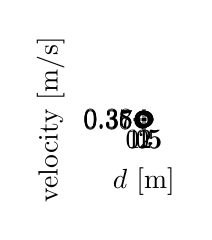
\begin{tikzpicture}

\begin{axis}[%
width=0.951\widthsette,
height=0.75\widthsette,
at={(0\widthsette,0\widthsette)},
scale only axis,
xmin=0,
xmax=2,
xlabel={$d$ [m]},
ymin=0.35,
ymax=0.38,
ylabel={velocity [m/s]},
axis background/.style={fill=white},
xmajorgrids,
ymajorgrids,
yticklabel style={/pgf/number format/.cd,fixed,precision=3}
]
\addplot [color=black, line width=1.0pt, mark size=2.5pt, mark=o, mark options={solid, black}, forget plot]
  table[row sep=crcr]{%
0.05	0.352715\\
0.2	0.371891\\
0.3	0.375066\\
0.5	0.376806\\
1	0.375925\\
1.5	0.374456\\
2	0.373188\\
};
\end{axis}
\end{tikzpicture}%
	\caption[Relation between the maximum velocity above the second cavity and 
	the distance between the cavities]{Relation between the maximum velocity in the peak above the second cavity and the distance $d$ between the cavities.}
	\label{fig:velpeaks}
\end{figure}
We see that if $d < d_{rec}$ the velocity is affected by the presence of 
the first cavity, reducing its value. For $d>d_{rec}$ the velocity is 
slightly decreasing as $d$ increases; this fact can be interpreted as the 
effect of the turbulence that 
is generated near the end of the first cavity. As it can be seen in 
Figure~\ref{fig:kd1}, the turbulent kinetic energy that is produced from the 
first cavity is transported towards the second one, leading to an increased 
thickness of the boundary layer as we move in the $x$-direction.
\begin{figure}
	\centering
	\includegraphics[width=\textwidth,% trim={0 0 0 7cm}, clip 
	]{cavities_dist1_k_report.png}
	\caption[Turbulen kinetic energy in the cavities problem]{Turbulent kinetic energy [$\si{m^2/s^2}$] around the cavities with $d=\SI{1}{m}$, at $t=T$. $Re=\num{6e5}$.}
	\label{fig:kd1}
\end{figure}
%
\subsubsection{Coupled problem with shallow cavities}
In this second test we simulate the same situation as in the previous 
single-domain test, 
choosing a distance between the two shallow cavities $d=\SI{1}{m}$, so that they do not influence each other directly. In addition to this, we couple the free-flow with the simulation of a flow inside a porous-medium that fills the space between 
the cavities, as it is shown in Figure~\ref{fig:multidomain}. In this way, we 
have two domains, $\Omega_\text{ff}$ and $\Omega_\text{pm}$, that are in contact through the 
interface $\Gamma_\text{int}$. The considered fluid is always isothermal, single-phase and single-component and gravity is neglected, as in the previous cases.

We want to analyse the differences that the presence of the porous-medium 
induces in the flow field with respect to the previous case and study how they 
change while we vary the permeability.

In the domain $\Omega_\text{ff}$ we solve, as before, the RANS equations with the 
$k\text{-}\omega$ model, while in the $\Omega_\text{pm}$ we solve the continuity equation
for a porous-medium flow \eqref{eq:pmcontinuity}, exploiting the Forchheimer's law \eqref{eq:forch}, in which we neglect the gravity contribution.
We use the same initial and boundary conditions we used before, but this time 
we have to impose, in addition, the coupling conditions described in 
Section~\ref{sec:coupling} on the interface 
$\Gamma_\text{int}$ and no-flow conditions on the boundary $\Gamma_\text{base}$, fixing the normal flux, i.e. the $v$ component of the velocity to zero.
We employ the same time discretization and the same grid we used before in $\Omega_\text{ff}$ and we extend it in 
$\Omega_\text{pm}$ in a conforming way.
\begin{figure}
	\centering
	\includegraphics[width=\textwidth]{cavities_multidomain_new.pdf}
	\caption[Domain change with respect to Figure~\ref{fig:singledomain} for the coupled problem with shallow cavities]{Domain change with respect to Figure~\ref{fig:singledomain} for the coupled problem with shallow cavities. The subdomain $\Omega_\text{pm}$ is introduced between the cavities.}
	\label{fig:multidomain}
\end{figure}

As we did in the previous case, we compare in Figure~\ref{fig:md_wall_velocities} the profiles of the $u$ component of the velocity at the position $y=h$ for several values of permeability. For values lower than $\SI{e-8}{m^2}$, the porous-medium results to be almost impermeable, or at least the flow field in $\Omega_\text{ff}$ is the 
same that we had in the previous test considering only the free-flow. The maximum velocities in the 
corner of the porous-medium are some orders of magnitude lower than those in 
the cavities (see Figure~\ref{fig:coupled_vel_3}).
\begin{figure}
	\centering
	\input{../img/cavities_coupled_velx_report}
	\caption[Profiles of the $u$ component of the velocity at $y=h$ in the coupled problem with shallow cavities]{Profiles of the $u$ component of the velocity at $y=h$ in the coupled problem with shallow cavities for several values of permeability, at $t=T$. $Re = \num{6e5}$.}
	\label{fig:md_wall_velocities}
\end{figure}
\begin{figure}
	\centering
	\includegraphics[width=\textwidth]{coupled_vel_3_report.png}
	\caption[Magnitude of the velocity field in the coupled problem with shallow cavities]{Magnitude of the velocity field $[\si{m/s}]$ in the coupled problem with shallow cavities, with $\mathrm{K}=\SI{3.1e-9}{m^2}$, at $t=T$. $Re=\num{6e5}$.}
	\label{fig:coupled_vel_3}
\end{figure}

Starting from $\mathrm{K}=\SI{3.1e-8}{m^2}$, we observe some changes in the velocity 
profile and increasing the permeability those changes are enhanced.
The increase of the maximum velocity in correspondence of the first cavity can 
be due to the reduction of the \emph{wall} behaviour of the porous-medium. The 
flow is allowed to reach higher velocities and it is less forced to reduce 
its velocity because a more relevant amount of fluid enters into the 
porous-medium (see Figure~\ref{fig:coupled_arrows}). Then this flow comes out 
from the top of $\Omega_\text{pm}$ within approximately the first 
$\SI{20}{cm}$; in the case of high permeability, this region with a peak in the 
$v$ component of the velocity spreads and 
moves a bit ahead, as it can be seen in Figure~\ref{fig:coupled_vel_split}.
\begin{figure}
	\centering
	\includegraphics[width=\textwidth]{coupled_first_cavity_report_labels.png}
	\caption[Velocity field near the end of the first cavity in the coupled problem with shallow cavities]{Velocity field [$\si{m/s}$] near the end of the first cavity in the coupled problem with shallow cavities, with $\mathrm{K}=\SI{3.1e-7}{m^2}$, at $t=T$. A portion of fluid enters into the porous-medium. The dashed line is the interface $\Gamma_\text{int}$. The length of the arrows is not scaled. $Re=\num{6e5}$.}
	\label{fig:coupled_arrows}
\end{figure}
\begin{figure}
	\centering
	\includegraphics[width=\textwidth]{coupled_split_comparison_report.png}
	\caption[$v$ component of the velocity near the end of the first cavity in the coupled problem with shallow cavities]{$v$ component of the velocity [$\si{m/s}$] near the end of the first cavity in the free-flow domain $\Omega_\text{ff}$, $t=T$. $\mathrm{K} = \SI{3.1e-7}{m^2}$ on the left and $\mathrm{K} = \SI{3.1e-9}{m^2}$ on the right. $Re=\num{6e5}$.}
	\label{fig:coupled_vel_split}
\end{figure}

After the distance $d_{rec}$, the value of the velocity that was there 
before the effect of the cavity is recovered and the boundary layer is 
restored. With high values of permeability this value is higher than the one 
with low permeabilities; this is due to the Beavers-Joseph-Saffman condition 
\eqref{eq:bjs} at the interface, that allows more slip as the permeability 
increases. Eventually the behaviour around the 
second cavity is approximately the same with all the permeabilities. There is a 
portion of fluid that goes back inside the porous-medium, but, since it comes 
from the corner eddy, the values involved are lower compared to what happens in 
the first cavity, so this effect does not seem to influence the free-flow 
notably (see Figure~\ref{fig:coupledsecondcav}).
\begin{figure}
	\centering
	\includegraphics[width=\textwidth]{coupled_second_cavity_report_labels.png}
	\caption[Velocity field near the beginning of the second cavity in the coupled problem with shallow cavities]{Velocity field $[\si{m/s}]$ near the beginning of the second cavity in the coupled problem with shallow cavities, with $\mathrm{K}=\SI{3.1e-7}{m^2}$ at $t=T$. Some flow enters into the porous medium. The dashed line is the interface $\Gamma_\text{int}$. The length of the arrows is not scaled. $Re=\num{6e5}$.}
	\label{fig:coupledsecondcav}
\end{figure}

%It is interesting to evaluate the mass flow rate $\dot{m}$ across the interface between the free-flow and the porous-medium flow. In particular, we compute, at $t=T$, the amount of mass that goes from the free-flow region to the porous-medium per unit of time as:
%\begin{equation}
%	\dot{m} = \int_{\Gamma_\text{int}} \max \{\varrho \mathbf{v} \cdot \mathbf{n}, 0 \} \; dA,
%\end{equation}
%where $\mathbf{n}$ is the outward unit vector normal to $\partial \Omega_\text{ff}$. From Table~\ref{tab:mass} and Figure~\ref{fig:mass} we can observe a relevant increase when the permeability is greater than $\SI{e-8}{m^2}$ approximately, so we find the same threshold value of the previous analysis.
%\begin{table}
%	\centering
%	\[
%	\begin{array}{cc}
%	\toprule
%	\mathrm{K} \; [\si{m^2}] & \dot{m} \; [\si{kg/s}]\\
%	\midrule
%	\num{3.1e-12} & \num{6.401e-4}\\
%	\num{3.1e-9} & \num{7.673e-4}\\
%	\num{3.1e-8} & \num{1.389e-3}\\
%	\num{1.55e-7} & \num{2.271e-3}\\
%	\num{3.1e-7} & \num{2.690e-3}\\
%	\num{3.1e-6} & \num{4.207e-3}\\
%	\bottomrule
%	\end{array}
%	\]
%	\caption[Mass flow rate across $\Gamma_\text{int}$ depending on the permeability in the coupled test with shallow cavities]{Mass flow rate from the free-flow region to the porous-medium across $\Gamma_\text{int}$, depending on the permeability, in the coupled test with shallow cavities.}
%	\label{tab:mass}
%\end{table}
%\begin{figure}
%	\centering
%	% This file was created by matlab2tikz.
%
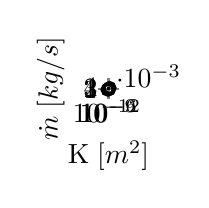
\begin{tikzpicture}

\begin{axis}[%
width=0.951\widthsei,
height=0.75\widthsei,
at={(0\widthsei,0\widthsei)},
scale only axis,
xmode=log,
xmin=1e-12,
xmax=0.00001,
xlabel={$\mathrm{K} \; [m^2]$},
ymin=0.0005,
ymax=0.0045,
ylabel={$\dot{m} \; [\si{kg/s}]$},
axis background/.style={fill=white},
xmajorgrids,
ymajorgrids
]
\addplot [color=black, line width=1.0pt, mark=o, mark options={solid, black}, forget plot]
  table[row sep=crcr]{%
3.1e-06	0.00420710161565\\
3.1e-07	0.002690450574475\\
1.55e-07	0.00227104284972\\
3.1e-08	0.0013892852915599\\
3.1e-09	0.0007673545670522\\
3.1e-12	0.000648090673435001\\
};
\end{axis}
\end{tikzpicture}%
%	\caption[Mass flow rate across $\Gamma_\text{int}$ depending on the permeability in the coupled test with shallow cavities]{Mass flow rate from the free-flow region to the porous-medium across $\Gamma_\text{int}$, depending on the permeability, in the coupled test with shallow cavities.}
%	\label{fig:mass}	
%\end{figure}
%
\subsubsection{Coupled problem with deep cavities}
We repeat the previous test considering the domain with deep cavities depicted in Figure~\ref{fig:multidomain_deep}, such that $h=\SI{0.3}{m}$. The grid is extended uniformly.
\begin{figure}
	\centering
	\includegraphics[width=\textwidth]{cavities_multidomain_deep.pdf}
	\caption[Domain change with respect to Figure~\ref{fig:singledomain} for the coupled problem with deep cavities]{Domain change with respect to Figure~\ref{fig:singledomain} for the coupled problem with deep cavities. The subdomain $\Omega_\text{pm}$ is introduced between the cavities.}
	\label{fig:multidomain_deep}
\end{figure}
Using the same model and the same boundary and interface conditions, we want to see if, with a different height of the cavities, the porous-medium flow affects differently the flow field. As before, we vary the permeability of the porous-medium in order to understand which is the threshold value between a permeable and an almost impermeable behaviour.

In Figure~\ref{fig:coupled_vel_deep}, we can see the magnitude of the velocity field in the region around the cavities and the porous-medium. As before, the two cavities show the same recirculation pattern, but it is different from the one that is generated when the cavities are shallow (see Figure~\ref{fig:coupled_vel_3}), because of the different size of the domain. Here, there is a bigger circular eddy touching the right boundary of the cavity and some smaller eddies in the left region of the cavity. 
\begin{figure}
	\centering
	\includegraphics[width=\textwidth]{coupled_deep_vel.png}
	\caption[Magnitude of the velocity field in the coupled problem with deep cavities]{Magnitude of the velocity field $[\si{m/s}]$ in the coupled problem with deep cavities, with $\mathrm{K}=\SI{3.1e-9}{m^2}$, at $t=T$. $Re=\num{6e5}$.}
	\label{fig:coupled_vel_deep}
\end{figure}

In Figure~\ref{fig:md_wall_velocities_deep}, we compare the profiles of the $u$ component of the velocity at the position $y=h$, for several values of permeability. With respect to Figure~\ref{fig:md_wall_velocities}, we observe a different profile in correspondence of the cavities, because of the different recirculation pattern inside them. As before, we notice that, as the permeability increases, the maximum velocity in correspondence of the first cavity increases, the minimum velocity above the beginning of the porous-medium decreases and the velocity above the end of the porous-medium increases. The threshold value for the permeability of approximately $\SI{e-8}{m^2}$ seems to be still valid. With respect to the previous test case, we observe that the value of the velocity before the second cavity, for $5 < x < 5.5$, increases faster. In fact, when $\mathrm{K} = \SI{3.1e-7}{m^2}$, it is greater than $\SI{0.3}{m/s}$, while in the previously, for the same value of permeability, it was approximately $\SI{0.27}{m/s}$. This fact could be due to a smaller amount of fluid exchanged with the porous-medium, or at least to differently distributed exchanges along the interface.
\begin{figure}
	\centering
	% This file was created by matlab2tikz.
%
\definecolor{mycolor1}{rgb}{0.00000,0.44700,0.74100}%
\definecolor{mycolor2}{rgb}{0.85000,0.32500,0.09800}%
\definecolor{mycolor3}{rgb}{0.92900,0.69400,0.12500}%
\definecolor{mycolor4}{rgb}{0.49400,0.18400,0.55600}%
\definecolor{mycolor5}{rgb}{0.46600,0.67400,0.18800}%
%
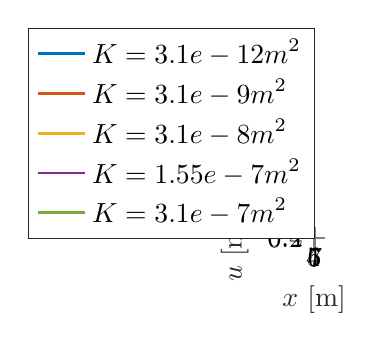
\begin{tikzpicture}

\begin{axis}[%
width=0.951\roughwidth,
height=0.75\roughwidth,
at={(0\roughwidth,0\roughwidth)},
scale only axis,
xmin=3.5,
xmax=7,
xlabel style={font=\color{white!15!black}},
xlabel={$x$ [m]},
ymin=0.05,
ymax=0.5,
ylabel style={font=\color{white!15!black}},
ylabel={$u$ [m/s]},
axis background/.style={fill=white},
xmajorgrids,
ymajorgrids,
legend style={at={(0.97,0.03)}, anchor=south east, legend cell align=left, align=left, draw=white!15!black}
]
\addplot [color=mycolor1, line width=1.0pt]
  table[row sep=crcr]{%
3.505	0.268641\\
3.51	0.268586\\
3.515	0.268586\\
3.52	0.268586\\
3.525	0.268586\\
3.53	0.268586\\
3.535	0.268586\\
3.54	0.268586\\
3.545	0.268586\\
3.55	0.268586\\
3.555	0.268586\\
3.56	0.268531\\
3.565	0.268531\\
3.57	0.268531\\
3.575	0.268531\\
3.58	0.268531\\
3.585	0.268531\\
3.59	0.268531\\
3.595	0.268531\\
3.6	0.268531\\
3.605	0.268478\\
3.61	0.268478\\
3.615	0.268478\\
3.62	0.268478\\
3.625	0.268478\\
3.63	0.268478\\
3.635	0.268478\\
3.64	0.268478\\
3.645	0.268425\\
3.65	0.268425\\
3.655	0.268425\\
3.66	0.268425\\
3.665	0.268425\\
3.67	0.268425\\
3.675	0.268425\\
3.68	0.268425\\
3.685	0.268372\\
3.69	0.268372\\
3.695	0.268372\\
3.7	0.268372\\
3.705	0.268372\\
3.71	0.268372\\
3.715	0.268372\\
3.72	0.268321\\
3.725	0.268321\\
3.73	0.268321\\
3.735	0.268321\\
3.74	0.268321\\
3.745	0.268321\\
3.75	0.268272\\
3.755	0.268272\\
3.76	0.268272\\
3.765	0.268272\\
3.77	0.268272\\
3.775	0.268224\\
3.78	0.268224\\
3.785	0.268224\\
3.79	0.268224\\
3.795	0.268224\\
3.8	0.268224\\
3.805	0.268179\\
3.81	0.268179\\
3.815	0.268179\\
3.82	0.268179\\
3.825	0.268138\\
3.83	0.268138\\
3.835	0.268138\\
3.84	0.268138\\
3.845	0.268101\\
3.85	0.268101\\
3.855	0.268101\\
3.86	0.268101\\
3.865	0.26807\\
3.87	0.26807\\
3.875	0.26807\\
3.88	0.26807\\
3.885	0.268046\\
3.89	0.268046\\
3.895	0.268046\\
3.9	0.268032\\
3.905	0.268032\\
3.91	0.268032\\
3.915	0.268029\\
3.92	0.268029\\
3.925	0.268039\\
3.93	0.268039\\
3.935	0.268039\\
3.94	0.268064\\
3.945	0.268064\\
3.95	0.268108\\
3.955	0.268108\\
3.96	0.268181\\
3.965	0.268181\\
3.97	0.268295\\
3.975	0.268475\\
3.98	0.268475\\
3.985	0.26877\\
3.99	0.269309\\
3.995	0.270665\\
4	0.274105\\
4.005	0.274105\\
4.01	0.279436\\
4.015	0.285139\\
4.02	0.290528\\
4.025	0.295444\\
4.03	0.299895\\
4.035	0.303921\\
4.04	0.307591\\
4.045	0.310975\\
4.05	0.314127\\
4.055	0.317085\\
4.06	0.319864\\
4.065	0.322474\\
4.07	0.324923\\
4.075	0.327221\\
4.08	0.329372\\
4.085	0.331373\\
4.09	0.333213\\
4.095	0.334873\\
4.1	0.336339\\
4.105	0.337595\\
4.11	0.33863\\
4.115	0.339432\\
4.12	0.339992\\
4.125	0.340318\\
4.13	0.3404\\
4.135	0.340279\\
4.14	0.340031\\
4.145	0.339684\\
4.15	0.339277\\
4.155	0.338864\\
4.16	0.338499\\
4.165	0.338234\\
4.17	0.338141\\
4.175	0.338261\\
4.18	0.338628\\
4.185	0.339312\\
4.19	0.340368\\
4.195	0.341836\\
4.2	0.343747\\
4.205	0.346097\\
4.21	0.348871\\
4.215	0.352029\\
4.22	0.355504\\
4.225	0.35924\\
4.23	0.363191\\
4.235	0.367317\\
4.24	0.371569\\
4.245	0.375903\\
4.25	0.380274\\
4.255	0.384626\\
4.26	0.38893\\
4.265	0.393176\\
4.27	0.397344\\
4.275	0.401417\\
4.28	0.405381\\
4.285	0.409227\\
4.29	0.412939\\
4.295	0.416502\\
4.3	0.41991\\
4.305	0.423155\\
4.31	0.426234\\
4.315	0.429146\\
4.32	0.431889\\
4.325	0.434465\\
4.33	0.43687\\
4.335	0.439103\\
4.34	0.441159\\
4.345	0.443038\\
4.35	0.444736\\
4.355	0.446254\\
4.36	0.447586\\
4.365	0.44873\\
4.37	0.44968\\
4.375	0.450431\\
4.38	0.45098\\
4.385	0.451315\\
4.39	0.451413\\
4.395	0.451268\\
4.4	0.450878\\
4.405	0.450214\\
4.41	0.449246\\
4.415	0.447941\\
4.42	0.446262\\
4.425	0.444163\\
4.43	0.441596\\
4.435	0.438511\\
4.44	0.434836\\
4.445	0.430464\\
4.45	0.425305\\
4.455	0.419253\\
4.46	0.412153\\
4.465	0.403835\\
4.47	0.394105\\
4.475	0.382743\\
4.48	0.369505\\
4.485	0.354102\\
4.49	0.336143\\
4.495	0.319023\\
4.5	0.333198\\
4.505	0.295534\\
4.51	0.21245\\
4.515	0.181175\\
4.52	0.174517\\
4.525	0.17893\\
4.53	0.187115\\
4.535	0.196196\\
4.54	0.204748\\
4.545	0.2124\\
4.55	0.2124\\
4.555	0.219105\\
4.56	0.224908\\
4.565	0.229904\\
4.57	0.229904\\
4.575	0.234241\\
4.58	0.238073\\
4.585	0.241469\\
4.59	0.241469\\
4.595	0.244489\\
4.6	0.247189\\
4.605	0.247189\\
4.61	0.249615\\
4.615	0.2518\\
4.62	0.2518\\
4.625	0.253771\\
4.63	0.253771\\
4.635	0.255553\\
4.64	0.257164\\
4.645	0.257164\\
4.65	0.258621\\
4.655	0.258621\\
4.66	0.259936\\
4.665	0.259936\\
4.67	0.261122\\
4.675	0.261122\\
4.68	0.26219\\
4.685	0.26315\\
4.69	0.26315\\
4.695	0.264012\\
4.7	0.264012\\
4.705	0.264783\\
4.71	0.264783\\
4.715	0.265471\\
4.72	0.265471\\
4.725	0.265471\\
4.73	0.266081\\
4.735	0.266081\\
4.74	0.266619\\
4.745	0.266619\\
4.75	0.267092\\
4.755	0.267092\\
4.76	0.267503\\
4.765	0.267503\\
4.77	0.267858\\
4.775	0.267858\\
4.78	0.267858\\
4.785	0.26816\\
4.79	0.26816\\
4.795	0.268416\\
4.8	0.268416\\
4.805	0.268416\\
4.81	0.268629\\
4.815	0.268629\\
4.82	0.268803\\
4.825	0.268803\\
4.83	0.268803\\
4.835	0.268943\\
4.84	0.268943\\
4.845	0.268943\\
4.85	0.269051\\
4.855	0.269051\\
4.86	0.269132\\
4.865	0.269132\\
4.87	0.269132\\
4.875	0.269186\\
4.88	0.269186\\
4.885	0.269186\\
4.89	0.269219\\
4.895	0.269219\\
4.9	0.269219\\
4.905	0.269228\\
4.91	0.269228\\
4.915	0.269228\\
4.92	0.269216\\
4.925	0.269216\\
4.93	0.269216\\
4.935	0.269188\\
4.94	0.269188\\
4.945	0.269188\\
4.95	0.269142\\
4.955	0.269142\\
4.96	0.269142\\
4.965	0.269142\\
4.97	0.269084\\
4.975	0.269084\\
4.98	0.269084\\
4.985	0.269018\\
4.99	0.269018\\
4.995	0.269018\\
5	0.269018\\
5.005	0.268946\\
5.01	0.268946\\
5.015	0.268946\\
5.02	0.268869\\
5.025	0.268869\\
5.03	0.268869\\
5.035	0.268792\\
5.04	0.268792\\
5.045	0.268792\\
5.05	0.268792\\
5.055	0.268716\\
5.06	0.268716\\
5.065	0.268716\\
5.07	0.268642\\
5.075	0.268642\\
5.08	0.268642\\
5.085	0.268571\\
5.09	0.268571\\
5.095	0.268571\\
5.1	0.268501\\
5.105	0.268501\\
5.11	0.268501\\
5.115	0.268433\\
5.12	0.268433\\
5.125	0.268433\\
5.13	0.268367\\
5.135	0.268367\\
5.14	0.268367\\
5.145	0.268302\\
5.15	0.268302\\
5.155	0.268238\\
5.16	0.268238\\
5.165	0.268238\\
5.17	0.268176\\
5.175	0.268176\\
5.18	0.268176\\
5.185	0.268116\\
5.19	0.268116\\
5.195	0.268057\\
5.2	0.268057\\
5.205	0.268057\\
5.21	0.268\\
5.215	0.268\\
5.22	0.267944\\
5.225	0.267944\\
5.23	0.267944\\
5.235	0.26789\\
5.24	0.26789\\
5.245	0.267837\\
5.25	0.267837\\
5.255	0.267785\\
5.26	0.267785\\
5.265	0.267736\\
5.27	0.267736\\
5.275	0.267687\\
5.28	0.267687\\
5.285	0.267687\\
5.29	0.26764\\
5.295	0.26764\\
5.3	0.267595\\
5.305	0.267595\\
5.31	0.267551\\
5.315	0.267551\\
5.32	0.267509\\
5.325	0.267468\\
5.33	0.267468\\
5.335	0.267429\\
5.34	0.267429\\
5.345	0.267391\\
5.35	0.267391\\
5.355	0.267355\\
5.36	0.267355\\
5.365	0.267321\\
5.37	0.267288\\
5.375	0.267288\\
5.38	0.267258\\
5.385	0.267258\\
5.39	0.26723\\
5.395	0.267204\\
5.4	0.267204\\
5.405	0.267181\\
5.41	0.267162\\
5.415	0.267162\\
5.42	0.267147\\
5.425	0.267136\\
5.43	0.267132\\
5.435	0.267132\\
5.44	0.267134\\
5.445	0.267144\\
5.45	0.267164\\
5.455	0.267164\\
5.46	0.267196\\
5.465	0.267245\\
5.47	0.267318\\
5.475	0.267425\\
5.48	0.267589\\
5.485	0.267853\\
5.49	0.268335\\
5.495	0.269531\\
5.5	0.272628\\
5.505	0.272628\\
5.51	0.277474\\
5.515	0.282668\\
5.52	0.287581\\
5.525	0.292068\\
5.53	0.296145\\
5.535	0.29984\\
5.54	0.303217\\
5.545	0.30634\\
5.55	0.309261\\
5.555	0.312008\\
5.56	0.314597\\
5.565	0.317038\\
5.57	0.319342\\
5.575	0.321522\\
5.58	0.323583\\
5.585	0.325521\\
5.59	0.327323\\
5.595	0.328971\\
5.6	0.330444\\
5.605	0.331723\\
5.61	0.332795\\
5.615	0.333644\\
5.62	0.334256\\
5.625	0.334633\\
5.63	0.334755\\
5.635	0.334648\\
5.64	0.33439\\
5.645	0.334012\\
5.65	0.333547\\
5.655	0.333046\\
5.66	0.332566\\
5.665	0.332159\\
5.67	0.331879\\
5.675	0.331796\\
5.68	0.331955\\
5.685	0.332395\\
5.69	0.333185\\
5.695	0.334373\\
5.7	0.335992\\
5.705	0.338059\\
5.71	0.340562\\
5.715	0.343477\\
5.72	0.346753\\
5.725	0.350324\\
5.73	0.354131\\
5.735	0.358126\\
5.74	0.362266\\
5.745	0.36651\\
5.75	0.370821\\
5.755	0.375143\\
5.76	0.379431\\
5.765	0.38366\\
5.77	0.387808\\
5.775	0.391861\\
5.78	0.395808\\
5.785	0.399635\\
5.79	0.403333\\
5.795	0.406893\\
5.8	0.410303\\
5.805	0.413554\\
5.81	0.416641\\
5.815	0.419561\\
5.82	0.422314\\
5.825	0.424898\\
5.83	0.427316\\
5.835	0.429563\\
5.84	0.431638\\
5.845	0.433538\\
5.85	0.435263\\
5.855	0.436809\\
5.86	0.438174\\
5.865	0.439353\\
5.87	0.440342\\
5.875	0.441134\\
5.88	0.441725\\
5.885	0.442104\\
5.89	0.442245\\
5.895	0.442144\\
5.9	0.441799\\
5.905	0.441181\\
5.91	0.440259\\
5.915	0.439002\\
5.92	0.437371\\
5.925	0.435322\\
5.93	0.432809\\
5.935	0.429783\\
5.94	0.426168\\
5.945	0.421856\\
5.95	0.416774\\
5.955	0.410818\\
5.96	0.403826\\
5.965	0.395636\\
5.97	0.38606\\
5.975	0.374887\\
5.98	0.361887\\
5.985	0.346792\\
5.99	0.329275\\
5.995	0.312749\\
6	0.327087\\
6.005	0.208078\\
6.01	0.208078\\
6.015	0.176608\\
6.02	0.171789\\
6.025	0.17932\\
6.03	0.17932\\
6.035	0.190726\\
6.04	0.202505\\
6.045	0.202505\\
6.05	0.213402\\
6.055	0.213402\\
6.06	0.222825\\
6.065	0.222825\\
6.07	0.230738\\
6.075	0.230738\\
6.08	0.237422\\
6.085	0.237422\\
6.09	0.237422\\
6.095	0.243093\\
6.1	0.243093\\
6.105	0.243093\\
6.11	0.24791\\
6.115	0.24791\\
6.12	0.24791\\
6.125	0.251995\\
6.13	0.251995\\
6.135	0.251995\\
6.14	0.255444\\
6.145	0.255444\\
6.15	0.255444\\
6.155	0.255444\\
6.16	0.25832\\
6.165	0.25832\\
6.17	0.25832\\
6.175	0.25832\\
6.18	0.260691\\
6.185	0.260691\\
6.19	0.260691\\
6.195	0.260691\\
6.2	0.260691\\
6.205	0.262604\\
6.21	0.262604\\
6.215	0.262604\\
6.22	0.262604\\
6.225	0.262604\\
6.23	0.264099\\
6.235	0.264099\\
6.24	0.264099\\
6.245	0.264099\\
6.25	0.264099\\
6.255	0.265227\\
6.26	0.265227\\
6.265	0.265227\\
6.27	0.265227\\
6.275	0.265227\\
6.28	0.265227\\
6.285	0.266039\\
6.29	0.266039\\
6.295	0.266039\\
6.3	0.266039\\
6.305	0.266039\\
6.31	0.266039\\
6.315	0.266039\\
6.32	0.266587\\
6.325	0.266587\\
6.33	0.266587\\
6.335	0.266587\\
6.34	0.266587\\
6.345	0.266587\\
6.35	0.266587\\
6.355	0.266587\\
6.36	0.266905\\
6.365	0.266905\\
6.37	0.266905\\
6.375	0.266905\\
6.38	0.266905\\
6.385	0.266905\\
6.39	0.266905\\
6.395	0.266905\\
6.4	0.267028\\
6.405	0.267028\\
6.41	0.267028\\
6.415	0.267028\\
6.42	0.267028\\
6.425	0.267028\\
6.43	0.267028\\
6.435	0.267028\\
6.44	0.267028\\
6.445	0.267016\\
6.45	0.267016\\
6.455	0.267016\\
6.46	0.267016\\
6.465	0.267016\\
6.47	0.267016\\
6.475	0.267016\\
6.48	0.267016\\
6.485	0.267016\\
6.49	0.26691\\
6.495	0.26691\\
6.5	0.26691\\
6.505	0.26691\\
6.51	0.26691\\
6.515	0.26691\\
6.52	0.26691\\
6.525	0.26691\\
6.53	0.26691\\
6.535	0.26691\\
6.54	0.26691\\
6.545	0.266738\\
6.55	0.266738\\
6.555	0.266738\\
6.56	0.266738\\
6.565	0.266738\\
6.57	0.266738\\
6.575	0.266738\\
6.58	0.266738\\
6.585	0.266738\\
6.59	0.266738\\
6.595	0.266738\\
6.6	0.266738\\
6.605	0.266527\\
6.61	0.266527\\
6.615	0.266527\\
6.62	0.266527\\
6.625	0.266527\\
6.63	0.266527\\
6.635	0.266527\\
6.64	0.266527\\
6.645	0.266527\\
6.65	0.266527\\
6.655	0.266527\\
6.66	0.266527\\
6.665	0.266527\\
6.67	0.266303\\
6.675	0.266303\\
6.68	0.266303\\
6.685	0.266303\\
6.69	0.266303\\
6.695	0.266303\\
6.7	0.266303\\
6.705	0.266303\\
6.71	0.266303\\
6.715	0.266303\\
6.72	0.266303\\
6.725	0.266303\\
6.73	0.266303\\
6.735	0.266303\\
6.74	0.266078\\
6.745	0.266078\\
6.75	0.266078\\
6.755	0.266078\\
6.76	0.266078\\
6.765	0.266078\\
6.77	0.266078\\
6.775	0.266078\\
6.78	0.266078\\
6.785	0.266078\\
6.79	0.266078\\
6.795	0.266078\\
6.8	0.266078\\
6.805	0.266078\\
6.81	0.266078\\
6.815	0.266078\\
6.82	0.265931\\
6.825	0.265931\\
6.83	0.265931\\
6.835	0.265931\\
6.84	0.265931\\
6.845	0.265931\\
6.85	0.265931\\
6.855	0.265931\\
6.86	0.265931\\
6.865	0.265931\\
6.87	0.265931\\
6.875	0.265931\\
6.88	0.265931\\
6.885	0.265931\\
6.89	0.265931\\
6.895	0.265931\\
6.9	0.265931\\
6.905	0.265846\\
6.91	0.265846\\
6.915	0.265846\\
6.92	0.265846\\
6.925	0.265846\\
6.93	0.265846\\
6.935	0.265846\\
6.94	0.265846\\
6.945	0.265846\\
6.95	0.265846\\
6.955	0.265846\\
6.96	0.265846\\
6.965	0.265846\\
6.97	0.265846\\
6.975	0.265846\\
6.98	0.265846\\
6.985	0.265846\\
6.99	0.265846\\
6.995	0.265846\\
7	0.265846\\
};
\addlegendentry{$\text{K = 3.1e-12 m}^\text{2}$}

\addplot [color=mycolor2, line width=1.0pt]
  table[row sep=crcr]{%
3.505	0.268642\\
3.51	0.268588\\
3.515	0.268588\\
3.52	0.268588\\
3.525	0.268588\\
3.53	0.268588\\
3.535	0.268588\\
3.54	0.268588\\
3.545	0.268588\\
3.55	0.268588\\
3.555	0.268588\\
3.56	0.268534\\
3.565	0.268534\\
3.57	0.268534\\
3.575	0.268534\\
3.58	0.268534\\
3.585	0.268534\\
3.59	0.268534\\
3.595	0.268534\\
3.6	0.268534\\
3.605	0.268481\\
3.61	0.268481\\
3.615	0.268481\\
3.62	0.268481\\
3.625	0.268481\\
3.63	0.268481\\
3.635	0.268481\\
3.64	0.268481\\
3.645	0.268429\\
3.65	0.268429\\
3.655	0.268429\\
3.66	0.268429\\
3.665	0.268429\\
3.67	0.268429\\
3.675	0.268429\\
3.68	0.268429\\
3.685	0.268377\\
3.69	0.268377\\
3.695	0.268377\\
3.7	0.268377\\
3.705	0.268377\\
3.71	0.268377\\
3.715	0.268377\\
3.72	0.268327\\
3.725	0.268327\\
3.73	0.268327\\
3.735	0.268327\\
3.74	0.268327\\
3.745	0.268327\\
3.75	0.268278\\
3.755	0.268278\\
3.76	0.268278\\
3.765	0.268278\\
3.77	0.268278\\
3.775	0.268232\\
3.78	0.268232\\
3.785	0.268232\\
3.79	0.268232\\
3.795	0.268232\\
3.8	0.268232\\
3.805	0.268188\\
3.81	0.268188\\
3.815	0.268188\\
3.82	0.268188\\
3.825	0.268148\\
3.83	0.268148\\
3.835	0.268148\\
3.84	0.268148\\
3.845	0.268113\\
3.85	0.268113\\
3.855	0.268113\\
3.86	0.268113\\
3.865	0.268083\\
3.87	0.268083\\
3.875	0.268083\\
3.88	0.268083\\
3.885	0.268061\\
3.89	0.268061\\
3.895	0.268061\\
3.9	0.268048\\
3.905	0.268048\\
3.91	0.268048\\
3.915	0.268047\\
3.92	0.268047\\
3.925	0.268059\\
3.93	0.268059\\
3.935	0.268059\\
3.94	0.268085\\
3.945	0.268085\\
3.95	0.268132\\
3.955	0.268132\\
3.96	0.268206\\
3.965	0.268206\\
3.97	0.268322\\
3.975	0.268504\\
3.98	0.268504\\
3.985	0.268801\\
3.99	0.269344\\
3.995	0.270705\\
4	0.274151\\
4.005	0.274151\\
4.01	0.279487\\
4.015	0.285197\\
4.02	0.290592\\
4.025	0.295515\\
4.03	0.299973\\
4.035	0.304008\\
4.04	0.307685\\
4.045	0.311076\\
4.05	0.314236\\
4.055	0.3172\\
4.06	0.319988\\
4.065	0.322605\\
4.07	0.325062\\
4.075	0.327368\\
4.08	0.329528\\
4.085	0.331538\\
4.09	0.333387\\
4.095	0.335058\\
4.1	0.336533\\
4.105	0.337799\\
4.11	0.338844\\
4.115	0.339654\\
4.12	0.340222\\
4.125	0.340554\\
4.13	0.340641\\
4.135	0.340522\\
4.14	0.340273\\
4.145	0.339923\\
4.15	0.339511\\
4.155	0.33909\\
4.16	0.338714\\
4.165	0.338436\\
4.17	0.338331\\
4.175	0.338437\\
4.18	0.338789\\
4.185	0.339457\\
4.19	0.340497\\
4.195	0.341952\\
4.2	0.34385\\
4.205	0.346191\\
4.21	0.34896\\
4.215	0.352119\\
4.22	0.355599\\
4.225	0.359343\\
4.23	0.363305\\
4.235	0.367444\\
4.24	0.371713\\
4.245	0.376063\\
4.25	0.380454\\
4.255	0.384826\\
4.26	0.38915\\
4.265	0.393416\\
4.27	0.397602\\
4.275	0.401694\\
4.28	0.405676\\
4.285	0.40954\\
4.29	0.413268\\
4.295	0.416848\\
4.3	0.420271\\
4.305	0.423531\\
4.31	0.426625\\
4.315	0.42955\\
4.32	0.432307\\
4.325	0.434894\\
4.33	0.437311\\
4.335	0.439555\\
4.34	0.441622\\
4.345	0.44351\\
4.35	0.445219\\
4.355	0.446745\\
4.36	0.448087\\
4.365	0.44924\\
4.37	0.450199\\
4.375	0.450959\\
4.38	0.451516\\
4.385	0.451861\\
4.39	0.451967\\
4.395	0.45183\\
4.4	0.45145\\
4.405	0.450796\\
4.41	0.449837\\
4.415	0.448543\\
4.42	0.446875\\
4.425	0.444789\\
4.43	0.442234\\
4.435	0.439162\\
4.44	0.435502\\
4.445	0.431151\\
4.45	0.426013\\
4.455	0.419984\\
4.46	0.412915\\
4.465	0.404636\\
4.47	0.394954\\
4.475	0.383653\\
4.48	0.370494\\
4.485	0.355196\\
4.49	0.337424\\
4.495	0.320063\\
4.5	0.3311\\
4.505	0.296933\\
4.51	0.218315\\
4.515	0.183282\\
4.52	0.173546\\
4.525	0.176179\\
4.53	0.183579\\
4.535	0.192723\\
4.54	0.201731\\
4.545	0.209995\\
4.55	0.209995\\
4.555	0.217385\\
4.56	0.223832\\
4.565	0.229415\\
4.57	0.229415\\
4.575	0.234267\\
4.58	0.238534\\
4.585	0.242312\\
4.59	0.242312\\
4.595	0.245666\\
4.6	0.248657\\
4.605	0.248657\\
4.61	0.251341\\
4.615	0.253754\\
4.62	0.253754\\
4.625	0.25593\\
4.63	0.25593\\
4.635	0.257894\\
4.64	0.25967\\
4.645	0.25967\\
4.65	0.261274\\
4.655	0.261274\\
4.66	0.262724\\
4.665	0.262724\\
4.67	0.264032\\
4.675	0.264032\\
4.68	0.265212\\
4.685	0.266275\\
4.69	0.266275\\
4.695	0.267231\\
4.7	0.267231\\
4.705	0.268088\\
4.71	0.268088\\
4.715	0.268855\\
4.72	0.268855\\
4.725	0.268855\\
4.73	0.269537\\
4.735	0.269537\\
4.74	0.270142\\
4.745	0.270142\\
4.75	0.270676\\
4.755	0.270676\\
4.76	0.271143\\
4.765	0.271143\\
4.77	0.271549\\
4.775	0.271549\\
4.78	0.271549\\
4.785	0.271899\\
4.79	0.271899\\
4.795	0.272198\\
4.8	0.272198\\
4.805	0.272198\\
4.81	0.272451\\
4.815	0.272451\\
4.82	0.272661\\
4.825	0.272661\\
4.83	0.272661\\
4.835	0.272834\\
4.84	0.272834\\
4.845	0.272834\\
4.85	0.272973\\
4.855	0.272973\\
4.86	0.27308\\
4.865	0.27308\\
4.87	0.27308\\
4.875	0.273159\\
4.88	0.273159\\
4.885	0.273159\\
4.89	0.273212\\
4.895	0.273212\\
4.9	0.273212\\
4.905	0.273243\\
4.91	0.273243\\
4.915	0.273243\\
4.92	0.27325\\
4.925	0.27325\\
4.93	0.27325\\
4.935	0.273237\\
4.94	0.273237\\
4.945	0.273237\\
4.95	0.273207\\
4.955	0.273207\\
4.96	0.273207\\
4.965	0.273207\\
4.97	0.273162\\
4.975	0.273162\\
4.98	0.273162\\
4.985	0.273107\\
4.99	0.273107\\
4.995	0.273107\\
5	0.273107\\
5.005	0.273043\\
5.01	0.273043\\
5.015	0.273043\\
5.02	0.272973\\
5.025	0.272973\\
5.03	0.272973\\
5.035	0.2729\\
5.04	0.2729\\
5.045	0.2729\\
5.05	0.2729\\
5.055	0.272827\\
5.06	0.272827\\
5.065	0.272827\\
5.07	0.272756\\
5.075	0.272756\\
5.08	0.272756\\
5.085	0.272686\\
5.09	0.272686\\
5.095	0.272686\\
5.1	0.272617\\
5.105	0.272617\\
5.11	0.272617\\
5.115	0.27255\\
5.12	0.27255\\
5.125	0.27255\\
5.13	0.272483\\
5.135	0.272483\\
5.14	0.272483\\
5.145	0.272418\\
5.15	0.272418\\
5.155	0.272355\\
5.16	0.272355\\
5.165	0.272355\\
5.17	0.272292\\
5.175	0.272292\\
5.18	0.272292\\
5.185	0.272232\\
5.19	0.272232\\
5.195	0.272172\\
5.2	0.272172\\
5.205	0.272172\\
5.21	0.272114\\
5.215	0.272114\\
5.22	0.272057\\
5.225	0.272057\\
5.23	0.272057\\
5.235	0.272002\\
5.24	0.272002\\
5.245	0.271949\\
5.25	0.271949\\
5.255	0.271896\\
5.26	0.271896\\
5.265	0.271845\\
5.27	0.271845\\
5.275	0.271796\\
5.28	0.271796\\
5.285	0.271796\\
5.29	0.271748\\
5.295	0.271748\\
5.3	0.271702\\
5.305	0.271702\\
5.31	0.271657\\
5.315	0.271657\\
5.32	0.271614\\
5.325	0.271572\\
5.33	0.271572\\
5.335	0.271531\\
5.34	0.271531\\
5.345	0.271492\\
5.35	0.271492\\
5.355	0.271454\\
5.36	0.271454\\
5.365	0.271418\\
5.37	0.271384\\
5.375	0.271384\\
5.38	0.271352\\
5.385	0.271352\\
5.39	0.271322\\
5.395	0.271294\\
5.4	0.271294\\
5.405	0.271269\\
5.41	0.271247\\
5.415	0.271247\\
5.42	0.271229\\
5.425	0.271215\\
5.43	0.271206\\
5.435	0.271206\\
5.44	0.271205\\
5.445	0.271211\\
5.45	0.271226\\
5.455	0.271226\\
5.46	0.271253\\
5.465	0.271296\\
5.47	0.271362\\
5.475	0.271462\\
5.48	0.271616\\
5.485	0.27187\\
5.49	0.272335\\
5.495	0.273479\\
5.5	0.27643\\
5.505	0.27643\\
5.51	0.281053\\
5.515	0.286015\\
5.52	0.290708\\
5.525	0.294992\\
5.53	0.298881\\
5.535	0.302406\\
5.54	0.305629\\
5.545	0.308615\\
5.55	0.31141\\
5.555	0.314041\\
5.56	0.316523\\
5.565	0.31887\\
5.57	0.321092\\
5.575	0.323202\\
5.58	0.325203\\
5.585	0.327092\\
5.59	0.328854\\
5.595	0.33047\\
5.6	0.331919\\
5.605	0.33318\\
5.61	0.334239\\
5.615	0.335079\\
5.62	0.335685\\
5.625	0.336057\\
5.63	0.336175\\
5.635	0.336063\\
5.64	0.335794\\
5.645	0.335403\\
5.65	0.334919\\
5.655	0.334394\\
5.66	0.333885\\
5.665	0.333442\\
5.67	0.333118\\
5.675	0.332991\\
5.68	0.333102\\
5.685	0.333483\\
5.69	0.334211\\
5.695	0.335333\\
5.7	0.336884\\
5.705	0.338882\\
5.71	0.341317\\
5.715	0.344167\\
5.72	0.347386\\
5.725	0.350905\\
5.73	0.354664\\
5.735	0.358615\\
5.74	0.362716\\
5.745	0.366923\\
5.75	0.3712\\
5.755	0.375499\\
5.76	0.379769\\
5.765	0.383983\\
5.77	0.388118\\
5.775	0.392159\\
5.78	0.396094\\
5.785	0.399911\\
5.79	0.403601\\
5.795	0.407154\\
5.8	0.41056\\
5.805	0.41381\\
5.81	0.416896\\
5.815	0.419817\\
5.82	0.42257\\
5.825	0.425155\\
5.83	0.427572\\
5.835	0.429821\\
5.84	0.4319\\
5.845	0.433806\\
5.85	0.435537\\
5.855	0.43709\\
5.86	0.438463\\
5.865	0.43965\\
5.87	0.440648\\
5.875	0.441449\\
5.88	0.44205\\
5.885	0.442439\\
5.89	0.442593\\
5.895	0.442506\\
5.9	0.442174\\
5.905	0.44157\\
5.91	0.440662\\
5.915	0.43942\\
5.92	0.437806\\
5.925	0.435772\\
5.93	0.433273\\
5.935	0.43026\\
5.94	0.426656\\
5.945	0.422358\\
5.95	0.417288\\
5.955	0.411343\\
5.96	0.404361\\
5.965	0.396177\\
5.97	0.386605\\
5.975	0.375429\\
5.98	0.362418\\
5.985	0.347303\\
5.99	0.329757\\
5.995	0.313202\\
6	0.327535\\
6.005	0.208277\\
6.01	0.208277\\
6.015	0.176677\\
6.02	0.171779\\
6.025	0.179283\\
6.03	0.179283\\
6.035	0.190688\\
6.04	0.202479\\
6.045	0.202479\\
6.05	0.213387\\
6.055	0.213387\\
6.06	0.222828\\
6.065	0.222828\\
6.07	0.230754\\
6.075	0.230754\\
6.08	0.237444\\
6.085	0.237444\\
6.09	0.237444\\
6.095	0.243123\\
6.1	0.243123\\
6.105	0.243123\\
6.11	0.247942\\
6.115	0.247942\\
6.12	0.247942\\
6.125	0.252027\\
6.13	0.252027\\
6.135	0.252027\\
6.14	0.255478\\
6.145	0.255478\\
6.15	0.255478\\
6.155	0.255478\\
6.16	0.258357\\
6.165	0.258357\\
6.17	0.258357\\
6.175	0.258357\\
6.18	0.260727\\
6.185	0.260727\\
6.19	0.260727\\
6.195	0.260727\\
6.2	0.260727\\
6.205	0.26264\\
6.21	0.26264\\
6.215	0.26264\\
6.22	0.26264\\
6.225	0.26264\\
6.23	0.264134\\
6.235	0.264134\\
6.24	0.264134\\
6.245	0.264134\\
6.25	0.264134\\
6.255	0.265257\\
6.26	0.265257\\
6.265	0.265257\\
6.27	0.265257\\
6.275	0.265257\\
6.28	0.265257\\
6.285	0.266067\\
6.29	0.266067\\
6.295	0.266067\\
6.3	0.266067\\
6.305	0.266067\\
6.31	0.266067\\
6.315	0.266067\\
6.32	0.266609\\
6.325	0.266609\\
6.33	0.266609\\
6.335	0.266609\\
6.34	0.266609\\
6.345	0.266609\\
6.35	0.266609\\
6.355	0.266609\\
6.36	0.266928\\
6.365	0.266928\\
6.37	0.266928\\
6.375	0.266928\\
6.38	0.266928\\
6.385	0.266928\\
6.39	0.266928\\
6.395	0.266928\\
6.4	0.267051\\
6.405	0.267051\\
6.41	0.267051\\
6.415	0.267051\\
6.42	0.267051\\
6.425	0.267051\\
6.43	0.267051\\
6.435	0.267051\\
6.44	0.267051\\
6.445	0.267032\\
6.45	0.267032\\
6.455	0.267032\\
6.46	0.267032\\
6.465	0.267032\\
6.47	0.267032\\
6.475	0.267032\\
6.48	0.267032\\
6.485	0.267032\\
6.49	0.266924\\
6.495	0.266924\\
6.5	0.266924\\
6.505	0.266924\\
6.51	0.266924\\
6.515	0.266924\\
6.52	0.266924\\
6.525	0.266924\\
6.53	0.266924\\
6.535	0.266924\\
6.54	0.266924\\
6.545	0.266749\\
6.55	0.266749\\
6.555	0.266749\\
6.56	0.266749\\
6.565	0.266749\\
6.57	0.266749\\
6.575	0.266749\\
6.58	0.266749\\
6.585	0.266749\\
6.59	0.266749\\
6.595	0.266749\\
6.6	0.266749\\
6.605	0.266538\\
6.61	0.266538\\
6.615	0.266538\\
6.62	0.266538\\
6.625	0.266538\\
6.63	0.266538\\
6.635	0.266538\\
6.64	0.266538\\
6.645	0.266538\\
6.65	0.266538\\
6.655	0.266538\\
6.66	0.266538\\
6.665	0.266538\\
6.67	0.266314\\
6.675	0.266314\\
6.68	0.266314\\
6.685	0.266314\\
6.69	0.266314\\
6.695	0.266314\\
6.7	0.266314\\
6.705	0.266314\\
6.71	0.266314\\
6.715	0.266314\\
6.72	0.266314\\
6.725	0.266314\\
6.73	0.266314\\
6.735	0.266314\\
6.74	0.266087\\
6.745	0.266087\\
6.75	0.266087\\
6.755	0.266087\\
6.76	0.266087\\
6.765	0.266087\\
6.77	0.266087\\
6.775	0.266087\\
6.78	0.266087\\
6.785	0.266087\\
6.79	0.266087\\
6.795	0.266087\\
6.8	0.266087\\
6.805	0.266087\\
6.81	0.266087\\
6.815	0.266087\\
6.82	0.265938\\
6.825	0.265938\\
6.83	0.265938\\
6.835	0.265938\\
6.84	0.265938\\
6.845	0.265938\\
6.85	0.265938\\
6.855	0.265938\\
6.86	0.265938\\
6.865	0.265938\\
6.87	0.265938\\
6.875	0.265938\\
6.88	0.265938\\
6.885	0.265938\\
6.89	0.265938\\
6.895	0.265938\\
6.9	0.265938\\
6.905	0.265851\\
6.91	0.265851\\
6.915	0.265851\\
6.92	0.265851\\
6.925	0.265851\\
6.93	0.265851\\
6.935	0.265851\\
6.94	0.265851\\
6.945	0.265851\\
6.95	0.265851\\
6.955	0.265851\\
6.96	0.265851\\
6.965	0.265851\\
6.97	0.265851\\
6.975	0.265851\\
6.98	0.265851\\
6.985	0.265851\\
6.99	0.265851\\
6.995	0.265851\\
7	0.265851\\
};
\addlegendentry{$\text{K = 3.1e-9 m}^\text{2}$}

\addplot [color=mycolor3, line width=1.0pt]
  table[row sep=crcr]{%
3.505	0.268647\\
3.51	0.268593\\
3.515	0.268593\\
3.52	0.268593\\
3.525	0.268593\\
3.53	0.268593\\
3.535	0.268593\\
3.54	0.268593\\
3.545	0.268593\\
3.55	0.268593\\
3.555	0.268593\\
3.56	0.268541\\
3.565	0.268541\\
3.57	0.268541\\
3.575	0.268541\\
3.58	0.268541\\
3.585	0.268541\\
3.59	0.268541\\
3.595	0.268541\\
3.6	0.268541\\
3.605	0.26849\\
3.61	0.26849\\
3.615	0.26849\\
3.62	0.26849\\
3.625	0.26849\\
3.63	0.26849\\
3.635	0.26849\\
3.64	0.26849\\
3.645	0.26844\\
3.65	0.26844\\
3.655	0.26844\\
3.66	0.26844\\
3.665	0.26844\\
3.67	0.26844\\
3.675	0.26844\\
3.68	0.26844\\
3.685	0.268391\\
3.69	0.268391\\
3.695	0.268391\\
3.7	0.268391\\
3.705	0.268391\\
3.71	0.268391\\
3.715	0.268391\\
3.72	0.268344\\
3.725	0.268344\\
3.73	0.268344\\
3.735	0.268344\\
3.74	0.268344\\
3.745	0.268344\\
3.75	0.268299\\
3.755	0.268299\\
3.76	0.268299\\
3.765	0.268299\\
3.77	0.268299\\
3.775	0.268256\\
3.78	0.268256\\
3.785	0.268256\\
3.79	0.268256\\
3.795	0.268256\\
3.8	0.268256\\
3.805	0.268216\\
3.81	0.268216\\
3.815	0.268216\\
3.82	0.268216\\
3.825	0.268179\\
3.83	0.268179\\
3.835	0.268179\\
3.84	0.268179\\
3.845	0.268148\\
3.85	0.268148\\
3.855	0.268148\\
3.86	0.268148\\
3.865	0.268124\\
3.87	0.268124\\
3.875	0.268124\\
3.88	0.268124\\
3.885	0.268106\\
3.89	0.268106\\
3.895	0.268106\\
3.9	0.268099\\
3.905	0.268099\\
3.91	0.268099\\
3.915	0.268104\\
3.92	0.268104\\
3.925	0.26812\\
3.93	0.26812\\
3.935	0.26812\\
3.94	0.268151\\
3.945	0.268151\\
3.95	0.268202\\
3.955	0.268202\\
3.96	0.268284\\
3.965	0.268284\\
3.97	0.268407\\
3.975	0.268597\\
3.98	0.268597\\
3.985	0.268902\\
3.99	0.269455\\
3.995	0.27083\\
4	0.274295\\
4.005	0.274295\\
4.01	0.279652\\
4.015	0.285383\\
4.02	0.2908\\
4.025	0.295746\\
4.03	0.30023\\
4.035	0.304289\\
4.04	0.30799\\
4.045	0.311405\\
4.05	0.314587\\
4.055	0.317574\\
4.06	0.320382\\
4.065	0.323022\\
4.07	0.325502\\
4.075	0.32783\\
4.08	0.330014\\
4.085	0.332047\\
4.09	0.333919\\
4.095	0.335613\\
4.1	0.337111\\
4.105	0.3384\\
4.11	0.339465\\
4.115	0.340295\\
4.12	0.34088\\
4.125	0.341224\\
4.13	0.341321\\
4.135	0.341205\\
4.14	0.340951\\
4.145	0.340595\\
4.15	0.34017\\
4.155	0.33973\\
4.16	0.339332\\
4.165	0.33903\\
4.17	0.338896\\
4.175	0.338973\\
4.18	0.3393\\
4.185	0.339945\\
4.19	0.340964\\
4.195	0.342401\\
4.2	0.344289\\
4.205	0.34663\\
4.21	0.34941\\
4.215	0.35259\\
4.22	0.356102\\
4.225	0.359886\\
4.23	0.363894\\
4.235	0.368084\\
4.24	0.372406\\
4.245	0.376815\\
4.25	0.381265\\
4.255	0.385696\\
4.26	0.390079\\
4.265	0.394402\\
4.27	0.398644\\
4.275	0.40279\\
4.28	0.406826\\
4.285	0.410739\\
4.29	0.414515\\
4.295	0.418141\\
4.3	0.421608\\
4.305	0.424909\\
4.31	0.428042\\
4.315	0.431005\\
4.32	0.433797\\
4.325	0.43642\\
4.33	0.43887\\
4.335	0.441144\\
4.34	0.443242\\
4.345	0.445161\\
4.35	0.446899\\
4.355	0.448454\\
4.36	0.449826\\
4.365	0.451009\\
4.37	0.451999\\
4.375	0.45279\\
4.38	0.453379\\
4.385	0.453757\\
4.39	0.453898\\
4.395	0.453798\\
4.4	0.453454\\
4.405	0.45284\\
4.41	0.451923\\
4.415	0.450673\\
4.42	0.449052\\
4.425	0.447015\\
4.43	0.444507\\
4.435	0.441476\\
4.44	0.437864\\
4.445	0.433585\\
4.45	0.428506\\
4.455	0.422536\\
4.46	0.415558\\
4.465	0.407369\\
4.47	0.397779\\
4.475	0.386573\\
4.48	0.373497\\
4.485	0.358229\\
4.49	0.340307\\
4.495	0.319839\\
4.5	0.315053\\
4.505	0.28666\\
4.51	0.222321\\
4.515	0.175632\\
4.52	0.151157\\
4.525	0.141463\\
4.53	0.140993\\
4.535	0.146046\\
4.54	0.15464\\
4.545	0.165124\\
4.55	0.165124\\
4.555	0.176257\\
4.56	0.187295\\
4.565	0.197566\\
4.57	0.197566\\
4.575	0.206865\\
4.58	0.215146\\
4.585	0.222479\\
4.59	0.222479\\
4.595	0.22899\\
4.6	0.234772\\
4.605	0.234772\\
4.61	0.239902\\
4.615	0.244463\\
4.62	0.244463\\
4.625	0.248536\\
4.63	0.248536\\
4.635	0.252182\\
4.64	0.25545\\
4.645	0.25545\\
4.65	0.258386\\
4.655	0.258386\\
4.66	0.261026\\
4.665	0.261026\\
4.67	0.263404\\
4.675	0.263404\\
4.68	0.265545\\
4.685	0.267472\\
4.69	0.267472\\
4.695	0.269208\\
4.7	0.269208\\
4.705	0.270769\\
4.71	0.270769\\
4.715	0.272172\\
4.72	0.272172\\
4.725	0.272172\\
4.73	0.273431\\
4.735	0.273431\\
4.74	0.274558\\
4.745	0.274558\\
4.75	0.275564\\
4.755	0.275564\\
4.76	0.27646\\
4.765	0.27646\\
4.77	0.277256\\
4.775	0.277256\\
4.78	0.277256\\
4.785	0.277959\\
4.79	0.277959\\
4.795	0.278579\\
4.8	0.278579\\
4.805	0.278579\\
4.81	0.279122\\
4.815	0.279122\\
4.82	0.279596\\
4.825	0.279596\\
4.83	0.279596\\
4.835	0.280005\\
4.84	0.280005\\
4.845	0.280005\\
4.85	0.280356\\
4.855	0.280356\\
4.86	0.280654\\
4.865	0.280654\\
4.87	0.280654\\
4.875	0.280904\\
4.88	0.280904\\
4.885	0.280904\\
4.89	0.281111\\
4.895	0.281111\\
4.9	0.281111\\
4.905	0.281278\\
4.91	0.281278\\
4.915	0.281278\\
4.92	0.28141\\
4.925	0.28141\\
4.93	0.28141\\
4.935	0.281511\\
4.94	0.281511\\
4.945	0.281511\\
4.95	0.281584\\
4.955	0.281584\\
4.96	0.281584\\
4.965	0.281584\\
4.97	0.281633\\
4.975	0.281633\\
4.98	0.281633\\
4.985	0.281663\\
4.99	0.281663\\
4.995	0.281663\\
5	0.281663\\
5.005	0.281673\\
5.01	0.281673\\
5.015	0.281673\\
5.02	0.281664\\
5.025	0.281664\\
5.03	0.281664\\
5.035	0.281643\\
5.04	0.281643\\
5.045	0.281643\\
5.05	0.281643\\
5.055	0.281611\\
5.06	0.281611\\
5.065	0.281611\\
5.07	0.281572\\
5.075	0.281572\\
5.08	0.281572\\
5.085	0.281528\\
5.09	0.281528\\
5.095	0.281528\\
5.1	0.281479\\
5.105	0.281479\\
5.11	0.281479\\
5.115	0.281428\\
5.12	0.281428\\
5.125	0.281428\\
5.13	0.281375\\
5.135	0.281375\\
5.14	0.281375\\
5.145	0.281321\\
5.15	0.281321\\
5.155	0.281267\\
5.16	0.281267\\
5.165	0.281267\\
5.17	0.281214\\
5.175	0.281214\\
5.18	0.281214\\
5.185	0.281161\\
5.19	0.281161\\
5.195	0.281108\\
5.2	0.281108\\
5.205	0.281108\\
5.21	0.281057\\
5.215	0.281057\\
5.22	0.281007\\
5.225	0.281007\\
5.23	0.281007\\
5.235	0.280958\\
5.24	0.280958\\
5.245	0.280911\\
5.25	0.280911\\
5.255	0.280864\\
5.26	0.280864\\
5.265	0.280819\\
5.27	0.280819\\
5.275	0.280775\\
5.28	0.280775\\
5.285	0.280775\\
5.29	0.280732\\
5.295	0.280732\\
5.3	0.28069\\
5.305	0.28069\\
5.31	0.280649\\
5.315	0.280649\\
5.32	0.28061\\
5.325	0.280571\\
5.33	0.280571\\
5.335	0.280533\\
5.34	0.280533\\
5.345	0.280497\\
5.35	0.280497\\
5.355	0.280461\\
5.36	0.280461\\
5.365	0.280427\\
5.37	0.280393\\
5.375	0.280393\\
5.38	0.280361\\
5.385	0.280361\\
5.39	0.280329\\
5.395	0.280299\\
5.4	0.280299\\
5.405	0.280271\\
5.41	0.280244\\
5.415	0.280244\\
5.42	0.280219\\
5.425	0.280196\\
5.43	0.280177\\
5.435	0.280177\\
5.44	0.280163\\
5.445	0.280154\\
5.45	0.280154\\
5.455	0.280154\\
5.46	0.280164\\
5.465	0.280187\\
5.47	0.28023\\
5.475	0.280305\\
5.48	0.280435\\
5.485	0.280671\\
5.49	0.281135\\
5.495	0.282172\\
5.5	0.284804\\
5.505	0.284804\\
5.51	0.288983\\
5.515	0.293476\\
5.52	0.297717\\
5.525	0.301572\\
5.53	0.305061\\
5.535	0.308217\\
5.54	0.311101\\
5.545	0.313775\\
5.55	0.316284\\
5.555	0.318647\\
5.56	0.320882\\
5.565	0.323006\\
5.57	0.325034\\
5.575	0.326976\\
5.58	0.328836\\
5.585	0.330607\\
5.59	0.332274\\
5.595	0.333815\\
5.6	0.335208\\
5.605	0.336429\\
5.61	0.337462\\
5.615	0.338288\\
5.62	0.338888\\
5.625	0.339256\\
5.63	0.339375\\
5.635	0.339262\\
5.64	0.338982\\
5.645	0.338569\\
5.65	0.338052\\
5.655	0.337481\\
5.66	0.33691\\
5.665	0.336394\\
5.67	0.335983\\
5.675	0.335739\\
5.68	0.335723\\
5.685	0.335978\\
5.69	0.336555\\
5.695	0.337513\\
5.7	0.338891\\
5.705	0.340712\\
5.71	0.342977\\
5.715	0.345661\\
5.72	0.348722\\
5.725	0.352103\\
5.73	0.355737\\
5.735	0.359573\\
5.74	0.363568\\
5.745	0.367682\\
5.75	0.371875\\
5.755	0.376108\\
5.76	0.380329\\
5.765	0.3845\\
5.77	0.388598\\
5.775	0.392604\\
5.78	0.396507\\
5.785	0.400297\\
5.79	0.403962\\
5.795	0.407495\\
5.8	0.410887\\
5.805	0.414128\\
5.81	0.417211\\
5.815	0.42013\\
5.82	0.422884\\
5.825	0.425471\\
5.83	0.42789\\
5.835	0.430141\\
5.84	0.432224\\
5.845	0.434138\\
5.85	0.435881\\
5.855	0.43745\\
5.86	0.43884\\
5.865	0.440047\\
5.87	0.441065\\
5.875	0.441889\\
5.88	0.442514\\
5.885	0.442928\\
5.89	0.443111\\
5.895	0.443055\\
5.9	0.44275\\
5.905	0.442176\\
5.91	0.441302\\
5.915	0.440096\\
5.92	0.438519\\
5.925	0.436522\\
5.93	0.434058\\
5.935	0.431078\\
5.94	0.427507\\
5.945	0.423243\\
5.95	0.418208\\
5.955	0.412296\\
5.96	0.405344\\
5.965	0.397188\\
5.97	0.387634\\
5.975	0.376464\\
5.98	0.363443\\
5.985	0.3483\\
5.99	0.330704\\
5.995	0.3141\\
6	0.328417\\
6.005	0.208553\\
6.01	0.208553\\
6.015	0.176651\\
6.02	0.171582\\
6.025	0.179034\\
6.03	0.179034\\
6.035	0.190453\\
6.04	0.202286\\
6.045	0.202286\\
6.05	0.21323\\
6.055	0.21323\\
6.06	0.22272\\
6.065	0.22272\\
6.07	0.230683\\
6.075	0.230683\\
6.08	0.237397\\
6.085	0.237397\\
6.09	0.237397\\
6.095	0.243098\\
6.1	0.243098\\
6.105	0.243098\\
6.11	0.247933\\
6.115	0.247933\\
6.12	0.247933\\
6.125	0.252031\\
6.13	0.252031\\
6.135	0.252031\\
6.14	0.255496\\
6.145	0.255496\\
6.15	0.255496\\
6.155	0.255496\\
6.16	0.258386\\
6.165	0.258386\\
6.17	0.258386\\
6.175	0.258386\\
6.18	0.260759\\
6.185	0.260759\\
6.19	0.260759\\
6.195	0.260759\\
6.2	0.260759\\
6.205	0.262677\\
6.21	0.262677\\
6.215	0.262677\\
6.22	0.262677\\
6.225	0.262677\\
6.23	0.264174\\
6.235	0.264174\\
6.24	0.264174\\
6.245	0.264174\\
6.25	0.264174\\
6.255	0.265297\\
6.26	0.265297\\
6.265	0.265297\\
6.27	0.265297\\
6.275	0.265297\\
6.28	0.265297\\
6.285	0.266107\\
6.29	0.266107\\
6.295	0.266107\\
6.3	0.266107\\
6.305	0.266107\\
6.31	0.266107\\
6.315	0.266107\\
6.32	0.266646\\
6.325	0.266646\\
6.33	0.266646\\
6.335	0.266646\\
6.34	0.266646\\
6.345	0.266646\\
6.35	0.266646\\
6.355	0.266646\\
6.36	0.266969\\
6.365	0.266969\\
6.37	0.266969\\
6.375	0.266969\\
6.38	0.266969\\
6.385	0.266969\\
6.39	0.266969\\
6.395	0.266969\\
6.4	0.267089\\
6.405	0.267089\\
6.41	0.267089\\
6.415	0.267089\\
6.42	0.267089\\
6.425	0.267089\\
6.43	0.267089\\
6.435	0.267089\\
6.44	0.267089\\
6.445	0.267058\\
6.45	0.267058\\
6.455	0.267058\\
6.46	0.267058\\
6.465	0.267058\\
6.47	0.267058\\
6.475	0.267058\\
6.48	0.267058\\
6.485	0.267058\\
6.49	0.266949\\
6.495	0.266949\\
6.5	0.266949\\
6.505	0.266949\\
6.51	0.266949\\
6.515	0.266949\\
6.52	0.266949\\
6.525	0.266949\\
6.53	0.266949\\
6.535	0.266949\\
6.54	0.266949\\
6.545	0.266772\\
6.55	0.266772\\
6.555	0.266772\\
6.56	0.266772\\
6.565	0.266772\\
6.57	0.266772\\
6.575	0.266772\\
6.58	0.266772\\
6.585	0.266772\\
6.59	0.266772\\
6.595	0.266772\\
6.6	0.266772\\
6.605	0.266562\\
6.61	0.266562\\
6.615	0.266562\\
6.62	0.266562\\
6.625	0.266562\\
6.63	0.266562\\
6.635	0.266562\\
6.64	0.266562\\
6.645	0.266562\\
6.65	0.266562\\
6.655	0.266562\\
6.66	0.266562\\
6.665	0.266562\\
6.67	0.266337\\
6.675	0.266337\\
6.68	0.266337\\
6.685	0.266337\\
6.69	0.266337\\
6.695	0.266337\\
6.7	0.266337\\
6.705	0.266337\\
6.71	0.266337\\
6.715	0.266337\\
6.72	0.266337\\
6.725	0.266337\\
6.73	0.266337\\
6.735	0.266337\\
6.74	0.266104\\
6.745	0.266104\\
6.75	0.266104\\
6.755	0.266104\\
6.76	0.266104\\
6.765	0.266104\\
6.77	0.266104\\
6.775	0.266104\\
6.78	0.266104\\
6.785	0.266104\\
6.79	0.266104\\
6.795	0.266104\\
6.8	0.266104\\
6.805	0.266104\\
6.81	0.266104\\
6.815	0.266104\\
6.82	0.265949\\
6.825	0.265949\\
6.83	0.265949\\
6.835	0.265949\\
6.84	0.265949\\
6.845	0.265949\\
6.85	0.265949\\
6.855	0.265949\\
6.86	0.265949\\
6.865	0.265949\\
6.87	0.265949\\
6.875	0.265949\\
6.88	0.265949\\
6.885	0.265949\\
6.89	0.265949\\
6.895	0.265949\\
6.9	0.265949\\
6.905	0.265859\\
6.91	0.265859\\
6.915	0.265859\\
6.92	0.265859\\
6.925	0.265859\\
6.93	0.265859\\
6.935	0.265859\\
6.94	0.265859\\
6.945	0.265859\\
6.95	0.265859\\
6.955	0.265859\\
6.96	0.265859\\
6.965	0.265859\\
6.97	0.265859\\
6.975	0.265859\\
6.98	0.265859\\
6.985	0.265859\\
6.99	0.265859\\
6.995	0.265859\\
7	0.265859\\
};
\addlegendentry{$\text{K = 3.1e-8 m}^\text{2}$}

\addplot [color=mycolor4, line width=1.0pt]
  table[row sep=crcr]{%
3.505	0.26865\\
3.51	0.268598\\
3.515	0.268598\\
3.52	0.268598\\
3.525	0.268598\\
3.53	0.268598\\
3.535	0.268598\\
3.54	0.268598\\
3.545	0.268598\\
3.55	0.268598\\
3.555	0.268598\\
3.56	0.268547\\
3.565	0.268547\\
3.57	0.268547\\
3.575	0.268547\\
3.58	0.268547\\
3.585	0.268547\\
3.59	0.268547\\
3.595	0.268547\\
3.6	0.268547\\
3.605	0.268498\\
3.61	0.268498\\
3.615	0.268498\\
3.62	0.268498\\
3.625	0.268498\\
3.63	0.268498\\
3.635	0.268498\\
3.64	0.268498\\
3.645	0.26845\\
3.65	0.26845\\
3.655	0.26845\\
3.66	0.26845\\
3.665	0.26845\\
3.67	0.26845\\
3.675	0.26845\\
3.68	0.26845\\
3.685	0.268403\\
3.69	0.268403\\
3.695	0.268403\\
3.7	0.268403\\
3.705	0.268403\\
3.71	0.268403\\
3.715	0.268403\\
3.72	0.268358\\
3.725	0.268358\\
3.73	0.268358\\
3.735	0.268358\\
3.74	0.268358\\
3.745	0.268358\\
3.75	0.268315\\
3.755	0.268315\\
3.76	0.268315\\
3.765	0.268315\\
3.77	0.268315\\
3.775	0.268275\\
3.78	0.268275\\
3.785	0.268275\\
3.79	0.268275\\
3.795	0.268275\\
3.8	0.268275\\
3.805	0.268238\\
3.81	0.268238\\
3.815	0.268238\\
3.82	0.268238\\
3.825	0.268206\\
3.83	0.268206\\
3.835	0.268206\\
3.84	0.268206\\
3.845	0.268179\\
3.85	0.268179\\
3.855	0.268179\\
3.86	0.268179\\
3.865	0.268158\\
3.87	0.268158\\
3.875	0.268158\\
3.88	0.268158\\
3.885	0.268145\\
3.89	0.268145\\
3.895	0.268145\\
3.9	0.268143\\
3.905	0.268143\\
3.91	0.268143\\
3.915	0.268151\\
3.92	0.268151\\
3.925	0.268171\\
3.93	0.268171\\
3.935	0.268171\\
3.94	0.268207\\
3.945	0.268207\\
3.95	0.268264\\
3.955	0.268264\\
3.96	0.268351\\
3.965	0.268351\\
3.97	0.268481\\
3.975	0.268677\\
3.98	0.268677\\
3.985	0.268989\\
3.99	0.269548\\
3.995	0.270934\\
4	0.274414\\
4.005	0.274414\\
4.01	0.279786\\
4.015	0.285535\\
4.02	0.290973\\
4.025	0.295942\\
4.03	0.300452\\
4.035	0.304535\\
4.04	0.308261\\
4.045	0.311699\\
4.05	0.314906\\
4.055	0.317915\\
4.06	0.320747\\
4.065	0.32341\\
4.07	0.325912\\
4.075	0.328263\\
4.08	0.330466\\
4.085	0.332516\\
4.09	0.334402\\
4.095	0.336105\\
4.1	0.337606\\
4.105	0.338892\\
4.11	0.339948\\
4.115	0.340761\\
4.12	0.341319\\
4.125	0.341625\\
4.13	0.341679\\
4.135	0.341521\\
4.14	0.341219\\
4.145	0.340809\\
4.15	0.340331\\
4.155	0.339841\\
4.16	0.3394\\
4.165	0.339065\\
4.17	0.338911\\
4.175	0.338987\\
4.18	0.339331\\
4.185	0.340016\\
4.19	0.341101\\
4.195	0.342633\\
4.2	0.344642\\
4.205	0.347125\\
4.21	0.350062\\
4.215	0.353409\\
4.22	0.35709\\
4.225	0.361046\\
4.23	0.365228\\
4.235	0.369587\\
4.24	0.374075\\
4.245	0.37864\\
4.25	0.383229\\
4.255	0.387788\\
4.26	0.392291\\
4.265	0.396728\\
4.27	0.401075\\
4.275	0.405318\\
4.28	0.409442\\
4.285	0.413434\\
4.29	0.41728\\
4.295	0.420966\\
4.3	0.424486\\
4.305	0.427836\\
4.31	0.431014\\
4.315	0.434019\\
4.32	0.436852\\
4.325	0.439513\\
4.33	0.441998\\
4.335	0.444305\\
4.34	0.446434\\
4.345	0.448385\\
4.35	0.450155\\
4.355	0.451745\\
4.36	0.453152\\
4.365	0.454374\\
4.37	0.455406\\
4.375	0.456244\\
4.38	0.456882\\
4.385	0.45731\\
4.39	0.457514\\
4.395	0.457477\\
4.4	0.457193\\
4.405	0.456646\\
4.41	0.455803\\
4.415	0.45463\\
4.42	0.453088\\
4.425	0.45113\\
4.43	0.4487\\
4.435	0.445736\\
4.44	0.442175\\
4.445	0.437953\\
4.45	0.432963\\
4.455	0.427054\\
4.46	0.420105\\
4.465	0.41195\\
4.47	0.402352\\
4.475	0.391059\\
4.48	0.377762\\
4.485	0.362049\\
4.49	0.343183\\
4.495	0.319369\\
4.5	0.299797\\
4.505	0.270719\\
4.51	0.219496\\
4.515	0.168853\\
4.52	0.132499\\
4.525	0.11024\\
4.53	0.0970263\\
4.535	0.0892063\\
4.54	0.0846338\\
4.545	0.0821368\\
4.55	0.0821368\\
4.555	0.0813081\\
4.56	0.08189\\
4.565	0.0835921\\
4.57	0.0835921\\
4.575	0.0866519\\
4.58	0.0912967\\
4.585	0.0974858\\
4.59	0.0974858\\
4.595	0.105265\\
4.6	0.114698\\
4.605	0.114698\\
4.61	0.125706\\
4.615	0.137968\\
4.62	0.137968\\
4.625	0.150927\\
4.63	0.150927\\
4.635	0.163962\\
4.64	0.176605\\
4.645	0.176605\\
4.65	0.188541\\
4.655	0.188541\\
4.66	0.199602\\
4.665	0.199602\\
4.67	0.209735\\
4.675	0.209735\\
4.68	0.218946\\
4.685	0.22728\\
4.69	0.22728\\
4.695	0.234794\\
4.7	0.234794\\
4.705	0.241539\\
4.71	0.241539\\
4.715	0.247563\\
4.72	0.247563\\
4.725	0.247563\\
4.73	0.25293\\
4.735	0.25293\\
4.74	0.25772\\
4.745	0.25772\\
4.75	0.262002\\
4.755	0.262002\\
4.76	0.265836\\
4.765	0.265836\\
4.77	0.269272\\
4.775	0.269272\\
4.78	0.269272\\
4.785	0.272357\\
4.79	0.272357\\
4.795	0.275127\\
4.8	0.275127\\
4.805	0.275127\\
4.81	0.277614\\
4.815	0.277614\\
4.82	0.279847\\
4.825	0.279847\\
4.83	0.279847\\
4.835	0.281849\\
4.84	0.281849\\
4.845	0.281849\\
4.85	0.283642\\
4.855	0.283642\\
4.86	0.285246\\
4.865	0.285246\\
4.87	0.285246\\
4.875	0.286677\\
4.88	0.286677\\
4.885	0.286677\\
4.89	0.287953\\
4.895	0.287953\\
4.9	0.287953\\
4.905	0.289085\\
4.91	0.289085\\
4.915	0.289085\\
4.92	0.290087\\
4.925	0.290087\\
4.93	0.290087\\
4.935	0.290971\\
4.94	0.290971\\
4.945	0.290971\\
4.95	0.291747\\
4.955	0.291747\\
4.96	0.291747\\
4.965	0.291747\\
4.97	0.292426\\
4.975	0.292426\\
4.98	0.292426\\
4.985	0.293019\\
4.99	0.293019\\
4.995	0.293019\\
5	0.293019\\
5.005	0.293529\\
5.01	0.293529\\
5.015	0.293529\\
5.02	0.293951\\
5.025	0.293951\\
5.03	0.293951\\
5.035	0.294297\\
5.04	0.294297\\
5.045	0.294297\\
5.05	0.294297\\
5.055	0.294582\\
5.06	0.294582\\
5.065	0.294582\\
5.07	0.294818\\
5.075	0.294818\\
5.08	0.294818\\
5.085	0.295011\\
5.09	0.295011\\
5.095	0.295011\\
5.1	0.295169\\
5.105	0.295169\\
5.11	0.295169\\
5.115	0.295298\\
5.12	0.295298\\
5.125	0.295298\\
5.13	0.295402\\
5.135	0.295402\\
5.14	0.295402\\
5.145	0.295485\\
5.15	0.295485\\
5.155	0.295551\\
5.16	0.295551\\
5.165	0.295551\\
5.17	0.295603\\
5.175	0.295603\\
5.18	0.295603\\
5.185	0.295642\\
5.19	0.295642\\
5.195	0.295671\\
5.2	0.295671\\
5.205	0.295671\\
5.21	0.295692\\
5.215	0.295692\\
5.22	0.295706\\
5.225	0.295706\\
5.23	0.295706\\
5.235	0.295714\\
5.24	0.295714\\
5.245	0.295717\\
5.25	0.295717\\
5.255	0.295715\\
5.26	0.295715\\
5.265	0.29571\\
5.27	0.29571\\
5.275	0.295703\\
5.28	0.295703\\
5.285	0.295703\\
5.29	0.295693\\
5.295	0.295693\\
5.3	0.295682\\
5.305	0.295682\\
5.31	0.295668\\
5.315	0.295668\\
5.32	0.295653\\
5.325	0.295637\\
5.33	0.295637\\
5.335	0.29562\\
5.34	0.29562\\
5.345	0.295602\\
5.35	0.295602\\
5.355	0.295582\\
5.36	0.295582\\
5.365	0.295562\\
5.37	0.29554\\
5.375	0.29554\\
5.38	0.295518\\
5.385	0.295518\\
5.39	0.295494\\
5.395	0.295469\\
5.4	0.295469\\
5.405	0.295443\\
5.41	0.295416\\
5.415	0.295416\\
5.42	0.295387\\
5.425	0.295357\\
5.43	0.295326\\
5.435	0.295326\\
5.44	0.295295\\
5.445	0.295264\\
5.45	0.295236\\
5.455	0.295236\\
5.46	0.295213\\
5.465	0.295198\\
5.47	0.295194\\
5.475	0.29521\\
5.48	0.295266\\
5.485	0.295415\\
5.49	0.295828\\
5.495	0.296681\\
5.5	0.29878\\
5.505	0.29878\\
5.51	0.302196\\
5.515	0.30588\\
5.52	0.309345\\
5.525	0.312462\\
5.53	0.315253\\
5.535	0.317758\\
5.54	0.320034\\
5.545	0.322139\\
5.55	0.324113\\
5.555	0.325975\\
5.56	0.327745\\
5.565	0.329444\\
5.57	0.331098\\
5.575	0.332718\\
5.58	0.334305\\
5.585	0.335848\\
5.59	0.337331\\
5.595	0.33873\\
5.6	0.340017\\
5.605	0.341164\\
5.61	0.34215\\
5.615	0.342954\\
5.62	0.343549\\
5.625	0.343926\\
5.63	0.344058\\
5.635	0.343956\\
5.64	0.343676\\
5.645	0.343243\\
5.65	0.342685\\
5.655	0.34205\\
5.66	0.34139\\
5.665	0.340756\\
5.67	0.340203\\
5.675	0.339783\\
5.68	0.339565\\
5.685	0.339601\\
5.69	0.33993\\
5.695	0.340613\\
5.7	0.3417\\
5.705	0.343221\\
5.71	0.345186\\
5.715	0.347577\\
5.72	0.350358\\
5.725	0.353483\\
5.73	0.356891\\
5.735	0.36052\\
5.74	0.36432\\
5.745	0.368255\\
5.75	0.372288\\
5.755	0.376379\\
5.76	0.380483\\
5.765	0.384564\\
5.77	0.388587\\
5.775	0.392522\\
5.78	0.396358\\
5.785	0.400085\\
5.79	0.403695\\
5.795	0.407178\\
5.8	0.410526\\
5.805	0.413735\\
5.81	0.416798\\
5.815	0.419704\\
5.82	0.42245\\
5.825	0.425032\\
5.83	0.427451\\
5.835	0.429704\\
5.84	0.431792\\
5.845	0.433713\\
5.85	0.435468\\
5.855	0.437056\\
5.86	0.438472\\
5.865	0.439711\\
5.87	0.440768\\
5.875	0.441635\\
5.88	0.442306\\
5.885	0.442771\\
5.89	0.443012\\
5.895	0.443015\\
5.9	0.442769\\
5.905	0.442259\\
5.91	0.441456\\
5.915	0.440325\\
5.92	0.438824\\
5.925	0.436905\\
5.93	0.434518\\
5.935	0.431612\\
5.94	0.428115\\
5.945	0.42393\\
5.95	0.418972\\
5.955	0.413135\\
5.96	0.40626\\
5.965	0.398173\\
5.97	0.388676\\
5.975	0.377542\\
5.98	0.364531\\
5.985	0.349369\\
5.99	0.331722\\
5.995	0.315049\\
6	0.32931\\
6.005	0.20868\\
6.01	0.20868\\
6.015	0.176328\\
6.02	0.170983\\
6.025	0.178355\\
6.03	0.178355\\
6.035	0.189802\\
6.04	0.201708\\
6.045	0.201708\\
6.05	0.21272\\
6.055	0.21272\\
6.06	0.222294\\
6.065	0.222294\\
6.07	0.230322\\
6.075	0.230322\\
6.08	0.23708\\
6.085	0.23708\\
6.09	0.23708\\
6.095	0.242818\\
6.1	0.242818\\
6.105	0.242818\\
6.11	0.247684\\
6.115	0.247684\\
6.12	0.247684\\
6.125	0.251813\\
6.13	0.251813\\
6.135	0.251813\\
6.14	0.255303\\
6.145	0.255303\\
6.15	0.255303\\
6.155	0.255303\\
6.16	0.258211\\
6.165	0.258211\\
6.17	0.258211\\
6.175	0.258211\\
6.18	0.260597\\
6.185	0.260597\\
6.19	0.260597\\
6.195	0.260597\\
6.2	0.260597\\
6.205	0.262527\\
6.21	0.262527\\
6.215	0.262527\\
6.22	0.262527\\
6.225	0.262527\\
6.23	0.264042\\
6.235	0.264042\\
6.24	0.264042\\
6.245	0.264042\\
6.25	0.264042\\
6.255	0.26518\\
6.26	0.26518\\
6.265	0.26518\\
6.27	0.26518\\
6.275	0.26518\\
6.28	0.26518\\
6.285	0.265994\\
6.29	0.265994\\
6.295	0.265994\\
6.3	0.265994\\
6.305	0.265994\\
6.31	0.265994\\
6.315	0.265994\\
6.32	0.266539\\
6.325	0.266539\\
6.33	0.266539\\
6.335	0.266539\\
6.34	0.266539\\
6.345	0.266539\\
6.35	0.266539\\
6.355	0.266539\\
6.36	0.266868\\
6.365	0.266868\\
6.37	0.266868\\
6.375	0.266868\\
6.38	0.266868\\
6.385	0.266868\\
6.39	0.266868\\
6.395	0.266868\\
6.4	0.266999\\
6.405	0.266999\\
6.41	0.266999\\
6.415	0.266999\\
6.42	0.266999\\
6.425	0.266999\\
6.43	0.266999\\
6.435	0.266999\\
6.44	0.266999\\
6.445	0.266979\\
6.45	0.266979\\
6.455	0.266979\\
6.46	0.266979\\
6.465	0.266979\\
6.47	0.266979\\
6.475	0.266979\\
6.48	0.266979\\
6.485	0.266979\\
6.49	0.266873\\
6.495	0.266873\\
6.5	0.266873\\
6.505	0.266873\\
6.51	0.266873\\
6.515	0.266873\\
6.52	0.266873\\
6.525	0.266873\\
6.53	0.266873\\
6.535	0.266873\\
6.54	0.266873\\
6.545	0.266704\\
6.55	0.266704\\
6.555	0.266704\\
6.56	0.266704\\
6.565	0.266704\\
6.57	0.266704\\
6.575	0.266704\\
6.58	0.266704\\
6.585	0.266704\\
6.59	0.266704\\
6.595	0.266704\\
6.6	0.266704\\
6.605	0.2665\\
6.61	0.2665\\
6.615	0.2665\\
6.62	0.2665\\
6.625	0.2665\\
6.63	0.2665\\
6.635	0.2665\\
6.64	0.2665\\
6.645	0.2665\\
6.65	0.2665\\
6.655	0.2665\\
6.66	0.2665\\
6.665	0.2665\\
6.67	0.266284\\
6.675	0.266284\\
6.68	0.266284\\
6.685	0.266284\\
6.69	0.266284\\
6.695	0.266284\\
6.7	0.266284\\
6.705	0.266284\\
6.71	0.266284\\
6.715	0.266284\\
6.72	0.266284\\
6.725	0.266284\\
6.73	0.266284\\
6.735	0.266284\\
6.74	0.266061\\
6.745	0.266061\\
6.75	0.266061\\
6.755	0.266061\\
6.76	0.266061\\
6.765	0.266061\\
6.77	0.266061\\
6.775	0.266061\\
6.78	0.266061\\
6.785	0.266061\\
6.79	0.266061\\
6.795	0.266061\\
6.8	0.266061\\
6.805	0.266061\\
6.81	0.266061\\
6.815	0.266061\\
6.82	0.265899\\
6.825	0.265899\\
6.83	0.265899\\
6.835	0.265899\\
6.84	0.265899\\
6.845	0.265899\\
6.85	0.265899\\
6.855	0.265899\\
6.86	0.265899\\
6.865	0.265899\\
6.87	0.265899\\
6.875	0.265899\\
6.88	0.265899\\
6.885	0.265899\\
6.89	0.265899\\
6.895	0.265899\\
6.9	0.265899\\
6.905	0.265812\\
6.91	0.265812\\
6.915	0.265812\\
6.92	0.265812\\
6.925	0.265812\\
6.93	0.265812\\
6.935	0.265812\\
6.94	0.265812\\
6.945	0.265812\\
6.95	0.265812\\
6.955	0.265812\\
6.96	0.265812\\
6.965	0.265812\\
6.97	0.265812\\
6.975	0.265812\\
6.98	0.265812\\
6.985	0.265812\\
6.99	0.265812\\
6.995	0.265812\\
7	0.265812\\
};
\addlegendentry{$\text{K = 1.55e-7 m}^\text{2}$}

\addplot [color=mycolor5, line width=1.0pt]
  table[row sep=crcr]{%
3.505	0.268654\\
3.51	0.268603\\
3.515	0.268603\\
3.52	0.268603\\
3.525	0.268603\\
3.53	0.268603\\
3.535	0.268603\\
3.54	0.268603\\
3.545	0.268603\\
3.55	0.268603\\
3.555	0.268603\\
3.56	0.268553\\
3.565	0.268553\\
3.57	0.268553\\
3.575	0.268553\\
3.58	0.268553\\
3.585	0.268553\\
3.59	0.268553\\
3.595	0.268553\\
3.6	0.268553\\
3.605	0.268505\\
3.61	0.268505\\
3.615	0.268505\\
3.62	0.268505\\
3.625	0.268505\\
3.63	0.268505\\
3.635	0.268505\\
3.64	0.268505\\
3.645	0.268459\\
3.65	0.268459\\
3.655	0.268459\\
3.66	0.268459\\
3.665	0.268459\\
3.67	0.268459\\
3.675	0.268459\\
3.68	0.268459\\
3.685	0.268414\\
3.69	0.268414\\
3.695	0.268414\\
3.7	0.268414\\
3.705	0.268414\\
3.71	0.268414\\
3.715	0.268414\\
3.72	0.268371\\
3.725	0.268371\\
3.73	0.268371\\
3.735	0.268371\\
3.74	0.268371\\
3.745	0.268371\\
3.75	0.268331\\
3.755	0.268331\\
3.76	0.268331\\
3.765	0.268331\\
3.77	0.268331\\
3.775	0.268294\\
3.78	0.268294\\
3.785	0.268294\\
3.79	0.268294\\
3.795	0.268294\\
3.8	0.268294\\
3.805	0.26826\\
3.81	0.26826\\
3.815	0.26826\\
3.82	0.26826\\
3.825	0.268232\\
3.83	0.268232\\
3.835	0.268232\\
3.84	0.268232\\
3.845	0.268208\\
3.85	0.268208\\
3.855	0.268208\\
3.86	0.268208\\
3.865	0.268192\\
3.87	0.268192\\
3.875	0.268192\\
3.88	0.268192\\
3.885	0.268184\\
3.89	0.268184\\
3.895	0.268184\\
3.9	0.268185\\
3.905	0.268185\\
3.91	0.268185\\
3.915	0.268198\\
3.92	0.268198\\
3.925	0.268222\\
3.93	0.268222\\
3.935	0.268222\\
3.94	0.268263\\
3.945	0.268263\\
3.95	0.268326\\
3.955	0.268326\\
3.96	0.268418\\
3.965	0.268418\\
3.97	0.268554\\
3.975	0.268757\\
3.98	0.268757\\
3.985	0.269076\\
3.99	0.269643\\
3.995	0.27104\\
4	0.274534\\
4.005	0.274534\\
4.01	0.279923\\
4.015	0.285692\\
4.02	0.291151\\
4.025	0.296145\\
4.03	0.300681\\
4.035	0.30479\\
4.04	0.308541\\
4.045	0.312006\\
4.05	0.315237\\
4.055	0.31827\\
4.06	0.321125\\
4.065	0.323812\\
4.07	0.326338\\
4.075	0.328712\\
4.08	0.330935\\
4.085	0.333003\\
4.09	0.334903\\
4.095	0.336616\\
4.1	0.338122\\
4.105	0.339407\\
4.11	0.340455\\
4.115	0.341252\\
4.12	0.341786\\
4.125	0.342056\\
4.13	0.342071\\
4.135	0.341873\\
4.14	0.341525\\
4.145	0.341065\\
4.15	0.340536\\
4.155	0.339999\\
4.16	0.339517\\
4.165	0.33915\\
4.17	0.338978\\
4.175	0.339053\\
4.18	0.339414\\
4.185	0.340138\\
4.19	0.341288\\
4.195	0.342912\\
4.2	0.345036\\
4.205	0.347654\\
4.21	0.350741\\
4.215	0.354244\\
4.22	0.358085\\
4.225	0.362202\\
4.23	0.366548\\
4.235	0.371066\\
4.24	0.375703\\
4.245	0.380412\\
4.25	0.385127\\
4.255	0.389799\\
4.26	0.394413\\
4.265	0.398952\\
4.27	0.403392\\
4.275	0.40772\\
4.28	0.411921\\
4.285	0.415981\\
4.29	0.419885\\
4.295	0.423622\\
4.3	0.427187\\
4.305	0.430577\\
4.31	0.433792\\
4.315	0.436832\\
4.32	0.439699\\
4.325	0.442389\\
4.33	0.4449\\
4.335	0.447232\\
4.34	0.449385\\
4.345	0.45136\\
4.35	0.453155\\
4.355	0.454772\\
4.36	0.456208\\
4.365	0.457462\\
4.37	0.45853\\
4.375	0.459405\\
4.38	0.460081\\
4.385	0.46055\\
4.39	0.460802\\
4.395	0.460811\\
4.4	0.460572\\
4.405	0.460074\\
4.41	0.459285\\
4.415	0.458169\\
4.42	0.456687\\
4.425	0.45479\\
4.43	0.452424\\
4.435	0.449522\\
4.44	0.446013\\
4.445	0.441829\\
4.45	0.436883\\
4.455	0.431052\\
4.46	0.42414\\
4.465	0.416006\\
4.47	0.406447\\
4.475	0.395139\\
4.48	0.381764\\
4.485	0.365871\\
4.49	0.346569\\
4.495	0.321468\\
4.5	0.298185\\
4.505	0.269655\\
4.51	0.224457\\
4.515	0.175826\\
4.52	0.136877\\
4.525	0.11122\\
4.53	0.0951938\\
4.535	0.0848837\\
4.54	0.0778796\\
4.545	0.0728212\\
4.55	0.0728212\\
4.555	0.0689867\\
4.56	0.0660548\\
4.565	0.0638909\\
4.57	0.0638909\\
4.575	0.0624231\\
4.58	0.0617306\\
4.585	0.0616889\\
4.59	0.0616889\\
4.595	0.062329\\
4.6	0.0639145\\
4.605	0.0639145\\
4.61	0.0664427\\
4.615	0.0699344\\
4.62	0.0699344\\
4.625	0.0744604\\
4.63	0.0744604\\
4.635	0.0801469\\
4.64	0.0871088\\
4.645	0.0871088\\
4.65	0.0954457\\
4.655	0.0954457\\
4.66	0.105242\\
4.665	0.105242\\
4.67	0.116493\\
4.675	0.116493\\
4.68	0.129041\\
4.685	0.142491\\
4.69	0.142491\\
4.695	0.156247\\
4.7	0.156247\\
4.705	0.169782\\
4.71	0.169782\\
4.715	0.182772\\
4.72	0.182772\\
4.725	0.182772\\
4.73	0.195004\\
4.735	0.195004\\
4.74	0.206375\\
4.745	0.206375\\
4.75	0.216871\\
4.755	0.216871\\
4.76	0.226511\\
4.765	0.226511\\
4.77	0.235296\\
4.775	0.235296\\
4.78	0.235296\\
4.785	0.243201\\
4.79	0.243201\\
4.795	0.250264\\
4.8	0.250264\\
4.805	0.250264\\
4.81	0.256581\\
4.815	0.256581\\
4.82	0.26224\\
4.825	0.26224\\
4.83	0.26224\\
4.835	0.267317\\
4.84	0.267317\\
4.845	0.267317\\
4.85	0.271874\\
4.855	0.271874\\
4.86	0.275969\\
4.865	0.275969\\
4.87	0.275969\\
4.875	0.279646\\
4.88	0.279646\\
4.885	0.279646\\
4.89	0.282945\\
4.895	0.282945\\
4.9	0.282945\\
4.905	0.285902\\
4.91	0.285902\\
4.915	0.285902\\
4.92	0.288548\\
4.925	0.288548\\
4.93	0.288548\\
4.935	0.290909\\
4.94	0.290909\\
4.945	0.290909\\
4.95	0.293012\\
4.955	0.293012\\
4.96	0.293012\\
4.965	0.293012\\
4.97	0.294882\\
4.975	0.294882\\
4.98	0.294882\\
4.985	0.29654\\
4.99	0.29654\\
4.995	0.29654\\
5	0.29654\\
5.005	0.297989\\
5.01	0.297989\\
5.015	0.297989\\
5.02	0.299222\\
5.025	0.299222\\
5.03	0.299222\\
5.035	0.30026\\
5.04	0.30026\\
5.045	0.30026\\
5.05	0.30026\\
5.055	0.301136\\
5.06	0.301136\\
5.065	0.301136\\
5.07	0.301879\\
5.075	0.301879\\
5.08	0.301879\\
5.085	0.302509\\
5.09	0.302509\\
5.095	0.302509\\
5.1	0.303044\\
5.105	0.303044\\
5.11	0.303044\\
5.115	0.303498\\
5.12	0.303498\\
5.125	0.303498\\
5.13	0.303883\\
5.135	0.303883\\
5.14	0.303883\\
5.145	0.30421\\
5.15	0.30421\\
5.155	0.304488\\
5.16	0.304488\\
5.165	0.304488\\
5.17	0.304724\\
5.175	0.304724\\
5.18	0.304724\\
5.185	0.304923\\
5.19	0.304923\\
5.195	0.305093\\
5.2	0.305093\\
5.205	0.305093\\
5.21	0.305236\\
5.215	0.305236\\
5.22	0.305357\\
5.225	0.305357\\
5.23	0.305357\\
5.235	0.305458\\
5.24	0.305458\\
5.245	0.305544\\
5.25	0.305544\\
5.255	0.305616\\
5.26	0.305616\\
5.265	0.305675\\
5.27	0.305675\\
5.275	0.305725\\
5.28	0.305725\\
5.285	0.305725\\
5.29	0.305766\\
5.295	0.305766\\
5.3	0.305799\\
5.305	0.305799\\
5.31	0.305826\\
5.315	0.305826\\
5.32	0.305847\\
5.325	0.305863\\
5.33	0.305863\\
5.335	0.305874\\
5.34	0.305874\\
5.345	0.305882\\
5.35	0.305882\\
5.355	0.305886\\
5.36	0.305886\\
5.365	0.305886\\
5.37	0.305883\\
5.375	0.305883\\
5.38	0.305878\\
5.385	0.305878\\
5.39	0.305868\\
5.395	0.305856\\
5.4	0.305856\\
5.405	0.30584\\
5.41	0.305821\\
5.415	0.305821\\
5.42	0.305798\\
5.425	0.305771\\
5.43	0.30574\\
5.435	0.30574\\
5.44	0.305706\\
5.445	0.30567\\
5.45	0.305632\\
5.455	0.305632\\
5.46	0.305595\\
5.465	0.305563\\
5.47	0.30554\\
5.475	0.305536\\
5.48	0.305565\\
5.485	0.305667\\
5.49	0.306018\\
5.495	0.306758\\
5.5	0.30856\\
5.505	0.30856\\
5.51	0.311493\\
5.515	0.314647\\
5.52	0.317593\\
5.525	0.320215\\
5.53	0.322533\\
5.535	0.324583\\
5.54	0.326425\\
5.545	0.328114\\
5.55	0.329681\\
5.555	0.331153\\
5.56	0.332558\\
5.565	0.333926\\
5.57	0.335282\\
5.575	0.336641\\
5.58	0.338004\\
5.585	0.33936\\
5.59	0.340689\\
5.595	0.341967\\
5.6	0.343163\\
5.605	0.344247\\
5.61	0.345192\\
5.615	0.345974\\
5.62	0.346566\\
5.625	0.346953\\
5.63	0.347102\\
5.635	0.347025\\
5.64	0.346757\\
5.645	0.346319\\
5.65	0.345747\\
5.655	0.345077\\
5.66	0.344361\\
5.665	0.343653\\
5.67	0.343004\\
5.675	0.342467\\
5.68	0.342096\\
5.685	0.341971\\
5.69	0.342132\\
5.695	0.34261\\
5.7	0.343474\\
5.705	0.344762\\
5.71	0.346489\\
5.715	0.348652\\
5.72	0.351211\\
5.725	0.354129\\
5.73	0.357358\\
5.735	0.360827\\
5.74	0.36448\\
5.745	0.368278\\
5.75	0.372187\\
5.755	0.376167\\
5.76	0.380177\\
5.765	0.384183\\
5.77	0.388149\\
5.775	0.39204\\
5.78	0.395834\\
5.785	0.399519\\
5.79	0.40309\\
5.795	0.406539\\
5.8	0.409857\\
5.805	0.413039\\
5.81	0.41608\\
5.815	0.418975\\
5.82	0.421716\\
5.825	0.424297\\
5.83	0.426716\\
5.835	0.428972\\
5.84	0.431064\\
5.845	0.432993\\
5.85	0.434756\\
5.855	0.436353\\
5.86	0.437781\\
5.865	0.439036\\
5.87	0.440114\\
5.875	0.441006\\
5.88	0.441706\\
5.885	0.442203\\
5.89	0.442482\\
5.895	0.442522\\
5.9	0.442315\\
5.905	0.441849\\
5.91	0.441092\\
5.915	0.440009\\
5.92	0.438556\\
5.925	0.436688\\
5.93	0.43435\\
5.935	0.431493\\
5.94	0.428047\\
5.945	0.423913\\
5.95	0.419008\\
5.955	0.413227\\
5.96	0.406409\\
5.965	0.398377\\
5.97	0.388926\\
5.975	0.37783\\
5.98	0.364843\\
5.985	0.34969\\
5.99	0.332032\\
5.995	0.315334\\
6	0.329553\\
6.005	0.208433\\
6.01	0.208433\\
6.015	0.175807\\
6.02	0.170295\\
6.025	0.177633\\
6.03	0.177633\\
6.035	0.189126\\
6.04	0.201107\\
6.045	0.201107\\
6.05	0.212189\\
6.055	0.212189\\
6.06	0.221833\\
6.065	0.221833\\
6.07	0.229918\\
6.075	0.229918\\
6.08	0.236718\\
6.085	0.236718\\
6.09	0.236718\\
6.095	0.242493\\
6.1	0.242493\\
6.105	0.242493\\
6.11	0.247388\\
6.115	0.247388\\
6.12	0.247388\\
6.125	0.251544\\
6.13	0.251544\\
6.135	0.251544\\
6.14	0.255053\\
6.145	0.255053\\
6.15	0.255053\\
6.155	0.255053\\
6.16	0.257981\\
6.165	0.257981\\
6.17	0.257981\\
6.175	0.257981\\
6.18	0.260384\\
6.185	0.260384\\
6.19	0.260384\\
6.195	0.260384\\
6.2	0.260384\\
6.205	0.262328\\
6.21	0.262328\\
6.215	0.262328\\
6.22	0.262328\\
6.225	0.262328\\
6.23	0.263858\\
6.235	0.263858\\
6.24	0.263858\\
6.245	0.263858\\
6.25	0.263858\\
6.255	0.265009\\
6.26	0.265009\\
6.265	0.265009\\
6.27	0.265009\\
6.275	0.265009\\
6.28	0.265009\\
6.285	0.265831\\
6.29	0.265831\\
6.295	0.265831\\
6.3	0.265831\\
6.305	0.265831\\
6.31	0.265831\\
6.315	0.265831\\
6.32	0.266387\\
6.325	0.266387\\
6.33	0.266387\\
6.335	0.266387\\
6.34	0.266387\\
6.345	0.266387\\
6.35	0.266387\\
6.355	0.266387\\
6.36	0.266722\\
6.365	0.266722\\
6.37	0.266722\\
6.375	0.266722\\
6.38	0.266722\\
6.385	0.266722\\
6.39	0.266722\\
6.395	0.266722\\
6.4	0.266867\\
6.405	0.266867\\
6.41	0.266867\\
6.415	0.266867\\
6.42	0.266867\\
6.425	0.266867\\
6.43	0.266867\\
6.435	0.266867\\
6.44	0.266867\\
6.445	0.266861\\
6.45	0.266861\\
6.455	0.266861\\
6.46	0.266861\\
6.465	0.266861\\
6.47	0.266861\\
6.475	0.266861\\
6.48	0.266861\\
6.485	0.266861\\
6.49	0.266761\\
6.495	0.266761\\
6.5	0.266761\\
6.505	0.266761\\
6.51	0.266761\\
6.515	0.266761\\
6.52	0.266761\\
6.525	0.266761\\
6.53	0.266761\\
6.535	0.266761\\
6.54	0.266761\\
6.545	0.266601\\
6.55	0.266601\\
6.555	0.266601\\
6.56	0.266601\\
6.565	0.266601\\
6.57	0.266601\\
6.575	0.266601\\
6.58	0.266601\\
6.585	0.266601\\
6.59	0.266601\\
6.595	0.266601\\
6.6	0.266601\\
6.605	0.266406\\
6.61	0.266406\\
6.615	0.266406\\
6.62	0.266406\\
6.625	0.266406\\
6.63	0.266406\\
6.635	0.266406\\
6.64	0.266406\\
6.645	0.266406\\
6.65	0.266406\\
6.655	0.266406\\
6.66	0.266406\\
6.665	0.266406\\
6.67	0.266199\\
6.675	0.266199\\
6.68	0.266199\\
6.685	0.266199\\
6.69	0.266199\\
6.695	0.266199\\
6.7	0.266199\\
6.705	0.266199\\
6.71	0.266199\\
6.715	0.266199\\
6.72	0.266199\\
6.725	0.266199\\
6.73	0.266199\\
6.735	0.266199\\
6.74	0.265984\\
6.745	0.265984\\
6.75	0.265984\\
6.755	0.265984\\
6.76	0.265984\\
6.765	0.265984\\
6.77	0.265984\\
6.775	0.265984\\
6.78	0.265984\\
6.785	0.265984\\
6.79	0.265984\\
6.795	0.265984\\
6.8	0.265984\\
6.805	0.265984\\
6.81	0.265984\\
6.815	0.265984\\
6.82	0.265826\\
6.825	0.265826\\
6.83	0.265826\\
6.835	0.265826\\
6.84	0.265826\\
6.845	0.265826\\
6.85	0.265826\\
6.855	0.265826\\
6.86	0.265826\\
6.865	0.265826\\
6.87	0.265826\\
6.875	0.265826\\
6.88	0.265826\\
6.885	0.265826\\
6.89	0.265826\\
6.895	0.265826\\
6.9	0.265826\\
6.905	0.265744\\
6.91	0.265744\\
6.915	0.265744\\
6.92	0.265744\\
6.925	0.265744\\
6.93	0.265744\\
6.935	0.265744\\
6.94	0.265744\\
6.945	0.265744\\
6.95	0.265744\\
6.955	0.265744\\
6.96	0.265744\\
6.965	0.265744\\
6.97	0.265744\\
6.975	0.265744\\
6.98	0.265744\\
6.985	0.265744\\
6.99	0.265744\\
6.995	0.265744\\
7	0.265744\\
};
\addlegendentry{$\text{K = 3.1e-7 m}^\text{2}$}

\end{axis}
\end{tikzpicture}%
	\caption[Profiles of the $u$ component of the velocity at $y=h$ in the coupled problem with deep cavities]{Profiles of the $u$ component of the velocity at $y=h$ in the coupled problem with deep cavities for several values of permeability, at $t=T$. $Re = \num{6e5}$.}
	\label{fig:md_wall_velocities_deep}
\end{figure}

In Figure~\ref{fig:coupled_first_deep} we see the velocity field around the first cavity. A portion of flow enters into the porous-medium near its upper-left corner, then it exits from above as in the case of shallow cavities.
The section of $\Gamma_\text{int}$ such that $y<h/2$ is characterized by a more complex behaviour for what concerns the flow direction. In fact, because of the multiple eddies, the exchange of fluid occurs both from the free-flow region to the porous-medium and vice versa.
In Figure~\ref{fig:coupledsecondcav_deep} we see the velocity field around the second cavity. Here, the flow pattern across the interface is analogous to the one in the case of shallow cavities, depicted in Figure~\ref{fig:coupledsecondcav}.
\begin{figure}
	\centering
	\includegraphics[width=\textwidth]{cav_deep_first3_labels.png}
	\caption[Velocity field around the first cavity in the coupled problem with deep cavities]{Velocity field [$\si{m/s}$] around the first cavity in the coupled problem with deep cavities, with $\mathrm{K}=\SI{3.1e-7}{m^2}$, at $t=T$. The dashed line is the interface $\Gamma_\text{int}$. The length of the arrows is not scaled. $Re=\num{6e5}$.}
	\label{fig:coupled_first_deep}
\end{figure}
\begin{figure}
	\centering
	\includegraphics[width=\textwidth]{cav_deep_second_labels.png}
	\caption[Velocity field around the second cavity in the coupled problem with deep cavities]{Velocity field $[\si{m/s}]$ around the second cavity in the coupled problem with deep cavities, with $\mathrm{K}=\SI{3.1e-7}{m^2}$ at $t=T$. The dashed line is the interface $\Gamma_\text{int}$. The length of the arrows is not scaled. $Re=\num{6e5}$.}
	\label{fig:coupledsecondcav_deep}
\end{figure}

It is interesting to evaluate the mass flow rate $\dot{m}$ across the interface between the free-flow and the porous-medium flow. In particular, we compute, at $t=T$, the amount of mass that goes from the free-flow region to the porous-medium per unit of time as:
\begin{equation}
\dot{m} = \int_{\Gamma_\text{int}} \max \{\varrho \mathbf{v} \cdot \mathbf{n}, 0 \} \; dA,
\end{equation}
where $\mathbf{n}$ is the outward unit vector normal to $\partial \Omega_\text{ff}$. Notice that, being the fluid incompressible and imposing no-flow conditions on the lower boundary of the porous-medium $\Gamma_\text{base}$, the net mass flow rate across $\Gamma_\text{int}$ is zero.

In Figure~\ref{fig:mass} we compare the values in the two cases of shallow and deep cavities. In both the situations we observe a relevant increase of the mass flow rate when the permeability is approximately greater than $\SI{e-8}{m^2}$, so the same threshold value that we found in the previous analysis. $\dot{m}$ is always greater in the case of deep cavities than in the case of shallow cavities. In Table~\ref{tab:mass} we compare the values and we compute the ratio $\dot{m}_\text{deep} / \dot{m}_\text{shallow}$, that results to be between $1.3$ and $1.5$ for every value of permeability. The ratio between the measure of the $\Gamma_\text{int}$ is $1.6 / 1.2 = 1.\bar{3}$, so it is likely that the difference in the mass flow rate between the two cases is simply due to the different extension of the interface.
\begin{figure}
	\centering
	\input{../img/mass_exchange_comp}
	\caption[Mass flow rate across $\Gamma_\text{int}$ depending on the permeability]{Mass flow rate from the free-flow region to the porous-medium across $\Gamma_\text{int}$, depending on the permeability.}
	\label{fig:mass}	
\end{figure}
\begin{table}
	\centering
	\[
	\begin{array}{cccc}
	\toprule
	\mathrm{K} \; [\si{m^2}] & \dot{m}_\text{deep} \; [\si{kg/s}] & \dot{m}_\text{shallow} \; [\si{kg/s}] & \dot{m}_\text{deep} / \dot{m}_\text{shallow}\\
	\midrule
	\num{3.1e-12} & \num{9.455e-4} & \num{6.401e-4} & 1.477\\
	\num{3.1e-9} & \num{1.083e-3} & \num{7.673e-4} & 1.411\\
	\num{3.1e-8} & \num{1.812e-3} & \num{1.389e-3} & 1.304\\
	\num{1.55e-7} & \num{3.063e-3} & \num{2.271e-3} & 1.349\\
	\num{3.1e-7} & \num{3.805e-3} & \num{2.690e-3} & 1.414\\
%	\num{3.1e-6} & \num{4.207e-3}\\
	\bottomrule
	\end{array}
	\]
	\caption[Mass flow rate across $\Gamma_\text{int}$ depending on the permeability]{Mass flow rate from the free-flow region to the porous-medium across $\Gamma_\text{int}$, depending on the permeability.}
	\label{tab:mass}
\end{table}
%\begin{table}
%	\centering
%	\[
%	\begin{array}{cc}
%	\toprule
%	\mathrm{K} \; [\si{m^2}] & \dot{m} \; [\si{kg/s}]\\
%	\midrule
%	\num{3.1e-12} & \num{9.455e-4}\\
%	\num{3.1e-9} & \num{1.083e-3}\\
%	\num{3.1e-8} & \num{1.812e-3}\\
%	\num{1.55e-7} & \num{3.063e-3}\\
%	\num{3.1e-7} & \num{3.805e-3}\\
%	\bottomrule
%	\end{array}
%	\]
%	\caption[Mass flow rate across $\Gamma_\text{int}$ depending on the permeability in the coupled test with deep cavities]{Mass flow rate from the free-flow region to the porous-medium across $\Gamma_\text{int}$, depending on the permeability, in the coupled test with deep cavities.}
%	\label{tab:mass_deep}
%\end{table}
%\begin{figure}
%	\centering
%	% This file was created by matlab2tikz.
%
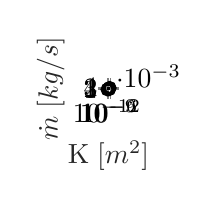
\begin{tikzpicture}

\begin{axis}[%
width=0.951\widthsei,
height=0.75\widthsei,
at={(0\widthsei,0\widthsei)},
scale only axis,
xmode=log,
xmin=1e-12,
xmax=1e-06,
xminorticks=true,
xlabel style={font=\color{white!15!black}},
xlabel={$\mathrm{K} \; [\si{m^2}]$},
ymin=0.0005,
ymax=0.004,
ylabel style={font=\color{white!15!black}},
ylabel={$\dot{m} \; [\si{kg/s}]$},
axis background/.style={fill=white},
xmajorgrids,
xminorgrids,
ymajorgrids
]
\addplot [color=black, line width=1.0pt, mark=o, mark options={solid, black}, forget plot]
  table[row sep=crcr]{%
3.1e-07	0.00380516439666\\
1.55e-07	0.00306263879357\\
3.1e-08	0.001811656088526\\
3.1e-09	0.00108318452159\\
3.1e-12	0.000945936611289998\\
};
\end{axis}
\end{tikzpicture}%
%	\caption[Mass flow rate across $\Gamma_\text{int}$ depending on the permeability in the coupled test with deep cavities]{Mass flow rate from the free-flow region to the porous-medium across $\Gamma_\text{int}$, depending on the permeability, in the coupled test with deep cavities.}
%	\label{fig:mass_deep}	
%\end{figure}
\subsection{Obstacle problem}
In this subsection we study the behaviour of
%an isothermal, single-phase, single-component
a turbulent flow in a channel with a porous obstacle of height $h=\SI{0.1}{m}$ on the lower boundary, as depicted in Figure~\ref{fig:obstacle_domain}. We want to analyse how the porous-medium affects the flow field, considering several possible values of permeability.
We solve the RANS equations \eqref{eq:ransmass}-\eqref{eq:ransmom} with the $k\text{-}\omega$ turbulence model \eqref{eq:komegak}-\eqref{eq:komegaomega} in the subdomain $\Omega_\text{ff}$ and the continuity equation for a porous-medium flow \eqref{eq:pmcontinuity}, exploiting the Forchheimer's law \eqref{eq:forch}, in the subdomain $\Omega_\text{pm}$. We neglect the gravity contributions.
\begin{figure}
	\centering
	\includegraphics[width=\textwidth]{obstacle_domain2.pdf}
	\caption[Domain for the obstacle problem]{Domain for the obstacle problem.}
	\label{fig:obstacle_domain}
\end{figure}
We impose inflow boundary conditions on the left boundary $\Gamma_\text{in}$:
\begin{equation}
\mathbf{v} = \mathbf{v}_\text{in} = [u_\text{in}, 0]^\mathrm{T}, \quad u_\text{in} = \SI{1}{m/s},
\end{equation}
no-slip boundary conditions on the lower boundary $\Gamma_w$, symmetry boundary conditions on the upper boundary $\Gamma_\text{sym}$ and outflow boundary conditions on the right boundary $\Gamma_\text{out}$, fixing the value of the pressure:
\begin{equation}
	p = p_\text{ext} = \SI{1.1e5}{\pascal}.
\end{equation}
On the interface $\Gamma_\text{int}$, we impose the coupling conditions described in Section~\ref{sec:coupling}, while on the boundary $\Gamma_\text{base}$ we impose no-flow conditions.
The density of the fluid is $\varrho = \SI{1}{kg/m^3}$ and its kinematic viscosity is $\nu=\SI{e-5}{m^2/s}$, so that the Reynolds number is $Re=\num{6e5}$. We start considering a permeability $\mathrm{K}=\SI{e-9}{m^2}.$ We simulate the time interval $(0,T) $, with $T=\SI{30}{s}$, such that the solution reaches an equilibrium, and we use an initial time-step $\Delta t = \SI{e-4}{s}$. As initial condition we set:
\begin{equation}
	\mathbf{v} = [u_\text{init}, 0]^\mathrm{T} \quad \forall \mathbf{x} \in \Omega_\text{ff}, \quad u_\text{init} =
	\begin{cases}
	u_\text{in} \quad&\text{if $x\leq 0 \lor x > \SI{1}{m}$}\\
	\frac{7}{6}u_\text{in} \quad&\text{if $0 \leq x \leq \SI{1}{m}$}\\
	\end{cases},
\end{equation}
\begin{equation}
	p = p_\text{ext} \quad \forall \mathbf{x} \in \Omega_\text{ff} \cup \Omega_\text{pm},
\end{equation}
\begin{equation}
	k = k_\text{in}, \; \omega = \omega_\text{in} \quad \forall \mathbf{x} \in \Omega_\text{ff}.
\end{equation}
The factor $7/6$ ensures that the flow rate is uniform along the channel.
Performing a sensitivity analysis, we choose a grid made of $\num{280x82}$ cells, employing gradings up to $1.2$ in order ho have refined cells near the walls. 
The size of the cells in the region around the upper-left corner of the obstacle shows to affect significantly the solution. In fact, looking at Figure~\ref{fig:obstacle_grid}, we can see how the pattern of the velocity field changes for three different grids.
\begin{figure}
	\centering
	\subfloat[]{\includegraphics[width=0.32\textwidth]{obstacle_grid4.png}\label{fig:grid4}}\hspace{0.008\textwidth}
	\subfloat[]{\includegraphics[width=0.32\textwidth]{obstacle_grid3.png}\label{fig:grid3}}\hspace{0.008\textwidth}
	\subfloat[]{\includegraphics[width=0.32\textwidth]{obstacle_grid2.png}\label{fig:grid2}}
	\caption[short text]{Magnitude of the velocity field $[\si{m/s}]$ near the beginning of the porous-medium, at $t=T$, considering a grid of
	\protect\subref{fig:grid4} $\num{207x52}$ cells, with minimum cell size at the obstacle corner equal to $\SI{3.3x4.4}{mm}$, 
	\protect\subref{fig:grid3} $\num{242x68}$ cells, with minimum cell size at the obstacle corner equal to $\SI{2x2.7}{mm}$,
	\protect\subref{fig:grid2} $\num{280x82}$ cells, with minimum cell size at the obstacle corner equal to $\SI{1.4x2}{mm}$.	
	$Re=\num{6e5}$.}
	\label{fig:obstacle_grid}
\end{figure}

In Figure~\ref{fig:obstacle_begin}, we can see the velocity field near the beginning of the porous obstacle. At the frontal face of the porous-medium, a small portion of the main flow enters into the obstacle, while the left amount of fluid recirculates near the bottom of the channel. At the corner of the porous-medium, the flow is deflected towards an higher region, so that, at the upper surface of the obstacle, a recirculation is generated and the velocity at the porous wall is negative.
In Figure~\ref{fig:obstacle_end}, we can see, instead, the velocity field near the end of the obstacle. The velocity pattern is analogous to the one generated by a backward facing step, as studied in Section~\ref{sec:bfs}. There is a small amount of fluid exiting from the porous-medium, but it does not seem to affect the eddies in the region after the obstacle.
\begin{figure}
	\centering
	\includegraphics[width=\textwidth]{obstacle_begin_vel_labels.png}
	\caption[Velocity field near the beginning of the obstacle in the obstacle problem]{Velocity field $[\si{m/s}]$ near the beginning of the obstacle in the obstacle problem, with $\mathrm{K} = \SI{e-9}{m^2}$ at $t=T$.
	The dashed line is the interface.
	The length of the arrows is not scaled. $Re = \num{6e5}$.}
	\label{fig:obstacle_begin}
\end{figure}
\begin{figure}
	\centering
	\includegraphics[width=\textwidth]{obstacle_end_vel2_labels.png}
	\caption[Velocity field near the end of the obstacle in the obstacle problem]{Velocity field $[\si{m/s}]$ near the end of the obstacle in the obstacle problem, with $\mathrm{K} = \SI{e-9}{m^2}$ at $t=T$.
	The dashed line is the interface.
	The length of the arrows is not scaled. $Re = \num{6e5}$.}
	\label{fig:obstacle_end}
\end{figure}

Now we analyse how a change in the permeability of the porous obstacle influences the flow field, considering a range from $\SI{e-11}{m^2}$ to $\SI{e-8}{m^2}$.

In Figure~\ref{fig:obstacle_diff} we can see the magnitude of the difference between the velocity field when $\mathrm{K}=\SI{e-8}{m^2}$ and $\mathrm{K}=\SI{e-11}{m^2}$. We observe that the most relevant differences are near the beginning of the obstacle, arising from the upper-left corner. Near the end of the obstacle, instead, the flow field is approximately the same.
\begin{figure}
	\centering
	\includegraphics[width=\textwidth]{obstacle_diff.png}
	\caption[Magnitude of the difference of the velocity field in the obstacle problem considering two values of permeability]{Magnitude of the difference of the velocity field $[\si{m/s}]$ in the obstacle problem between the cases $\mathrm{K}=\SI{e-8}{m^2}$ and $\mathrm{K}=\SI{e-11}{m^2}$.}
	\label{fig:obstacle_diff}
\end{figure}
\begin{figure}
	\centering
	\subfloat[$u$ component]{\includegraphics[width=0.4\textwidth]{obstacle_pm_diff_x.png}}\hspace{2cm}
	\subfloat[$v$ component]{\includegraphics[width=0.4\textwidth]{obstacle_pm_diff_y.png}}
	\caption[Difference of the velocity field at the beginning of the porous obstacle between two values of permeability]{Components of the difference $\mathbf{v}_8 - \mathbf{v}_{11}$ $[\si{m/s}]$ at the beginning of the porous obstacle, where $\mathbf{v}_n$ is the velocity field computed considering a permeability $\mathrm{K}=10^{-n}\;\si{m^2}$.}
	\label{fig:obstacle_pm_diff}
\end{figure}
\begin{figure}
	\centering
	% This file was created by matlab2tikz.
%
\definecolor{mycolor1}{rgb}{0.00000,0.44700,0.74100}%
\definecolor{mycolor2}{rgb}{0.85000,0.32500,0.09800}%
\definecolor{mycolor3}{rgb}{0.92900,0.69400,0.12500}%
\definecolor{mycolor4}{rgb}{0.49400,0.18400,0.55600}%
%
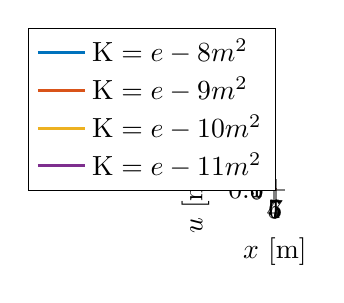
\begin{tikzpicture}

\begin{axis}[%
width=0.931\roughwidth,
height=0.75\roughwidth,
at={(0\roughwidth,0\roughwidth)},
scale only axis,
xmin=4,
xmax=7,
xlabel={$x$ [m]},
ymin=-0.4,
ymax=1,
ylabel={$u$ [m/s]},
axis background/.style={fill=white},
xmajorgrids,
ymajorgrids,
legend style={at={(0.97,0.03)}, anchor=south east, legend cell align=left, align=left}
]
\addplot [color=mycolor1, line width=1.0pt]
  table[row sep=crcr]{%
4.005	0.971278\\
4.01	0.971278\\
4.015	0.963829\\
4.02	0.963829\\
4.025	0.963829\\
4.03	0.963829\\
4.035	0.963829\\
4.04	0.963829\\
4.045	0.963829\\
4.05	0.963829\\
4.055	0.955812\\
4.06	0.955812\\
4.065	0.955812\\
4.07	0.955812\\
4.075	0.955812\\
4.08	0.955812\\
4.085	0.955812\\
4.09	0.955812\\
4.095	0.947341\\
4.1	0.947341\\
4.105	0.947341\\
4.11	0.947341\\
4.115	0.947341\\
4.12	0.947341\\
4.125	0.938542\\
4.13	0.938542\\
4.135	0.938542\\
4.14	0.938542\\
4.145	0.938542\\
4.15	0.938542\\
4.155	0.938542\\
4.16	0.929543\\
4.165	0.929543\\
4.17	0.929543\\
4.175	0.929543\\
4.18	0.929543\\
4.185	0.920459\\
4.19	0.920459\\
4.195	0.920459\\
4.2	0.920459\\
4.205	0.920459\\
4.21	0.911387\\
4.215	0.911387\\
4.22	0.911387\\
4.225	0.911387\\
4.23	0.911387\\
4.235	0.902395\\
4.24	0.902395\\
4.245	0.902395\\
4.25	0.902395\\
4.255	0.893525\\
4.26	0.893525\\
4.265	0.893525\\
4.27	0.893525\\
4.275	0.884798\\
4.28	0.884798\\
4.285	0.884798\\
4.29	0.876222\\
4.295	0.876222\\
4.3	0.876222\\
4.305	0.876222\\
4.31	0.867798\\
4.315	0.867798\\
4.32	0.867798\\
4.325	0.859525\\
4.33	0.859525\\
4.335	0.851404\\
4.34	0.851404\\
4.345	0.851404\\
4.35	0.843439\\
4.355	0.843439\\
4.36	0.835633\\
4.365	0.835633\\
4.37	0.827996\\
4.375	0.820534\\
4.38	0.820534\\
4.385	0.813256\\
4.39	0.813256\\
4.395	0.80617\\
4.4	0.799283\\
4.405	0.792602\\
4.41	0.786133\\
4.415	0.779882\\
4.42	0.773854\\
4.425	0.768054\\
4.43	0.762487\\
4.435	0.752063\\
4.44	0.742597\\
4.445	0.734087\\
4.45	0.723063\\
4.455	0.709167\\
4.46	0.69751\\
4.465	0.679862\\
4.47	0.664666\\
4.475	0.641016\\
4.48	0.619969\\
4.485	0.585792\\
4.49	0.553818\\
4.495	0.499223\\
4.5	0.481872\\
4.505	-0.0202071\\
4.51	-0.0211152\\
4.515	-0.0129989\\
4.52	-0.0119704\\
4.525	-0.0114417\\
4.53	-0.011642\\
4.535	-0.0119477\\
4.54	-0.011849\\
4.545	-0.0112694\\
4.55	-0.010725\\
4.555	-0.0103837\\
4.56	-0.0106751\\
4.565	-0.012533\\
4.57	-0.0136381\\
4.575	-0.0168317\\
4.58	-0.021873\\
4.585	-0.0295879\\
4.59	-0.0346527\\
4.595	-0.0474363\\
4.6	-0.0551928\\
4.605	-0.0638414\\
4.61	-0.0733259\\
4.615	-0.0943503\\
4.62	-0.105503\\
4.625	-0.116783\\
4.63	-0.127969\\
4.635	-0.138869\\
4.64	-0.149338\\
4.645	-0.15928\\
4.65	-0.15928\\
4.655	-0.168638\\
4.66	-0.17738\\
4.665	-0.185475\\
4.67	-0.192901\\
4.675	-0.192901\\
4.68	-0.199632\\
4.685	-0.20564\\
4.69	-0.210873\\
4.695	-0.210873\\
4.7	-0.215304\\
4.705	-0.218925\\
4.71	-0.218925\\
4.715	-0.221638\\
4.72	-0.221638\\
4.725	-0.223352\\
4.73	-0.224116\\
4.735	-0.224116\\
4.74	-0.223729\\
4.745	-0.223729\\
4.75	-0.222037\\
4.755	-0.222037\\
4.76	-0.21909\\
4.765	-0.21909\\
4.77	-0.214819\\
4.775	-0.214819\\
4.78	-0.209156\\
4.785	-0.209156\\
4.79	-0.202025\\
4.795	-0.202025\\
4.8	-0.202025\\
4.805	-0.193364\\
4.81	-0.193364\\
4.815	-0.183091\\
4.82	-0.183091\\
4.825	-0.183091\\
4.83	-0.171144\\
4.835	-0.171144\\
4.84	-0.157518\\
4.845	-0.157518\\
4.85	-0.157518\\
4.855	-0.142288\\
4.86	-0.142288\\
4.865	-0.142288\\
4.87	-0.125585\\
4.875	-0.125585\\
4.88	-0.125585\\
4.885	-0.107542\\
4.89	-0.107542\\
4.895	-0.107542\\
4.9	-0.0882953\\
4.905	-0.0882953\\
4.91	-0.0882953\\
4.915	-0.0679799\\
4.92	-0.0679799\\
4.925	-0.0679799\\
4.93	-0.0468296\\
4.935	-0.0468296\\
4.94	-0.0468296\\
4.945	-0.0250677\\
4.95	-0.0250677\\
4.955	-0.0250677\\
4.96	-0.0250677\\
4.965	-0.00285304\\
4.97	-0.00285304\\
4.975	-0.00285304\\
4.98	-0.00285304\\
4.985	0.0197347\\
4.99	0.0197347\\
4.995	0.0197347\\
5	0.0197347\\
5.005	0.0427833\\
5.01	0.0427833\\
5.015	0.0427833\\
5.02	0.0427833\\
5.025	0.0649641\\
5.03	0.0649641\\
5.035	0.0649641\\
5.04	0.0649641\\
5.045	0.0850924\\
5.05	0.0850924\\
5.055	0.0850924\\
5.06	0.103425\\
5.065	0.103425\\
5.07	0.103425\\
5.075	0.103425\\
5.08	0.120061\\
5.085	0.120061\\
5.09	0.120061\\
5.095	0.120061\\
5.1	0.135104\\
5.105	0.135104\\
5.11	0.135104\\
5.115	0.148684\\
5.12	0.148684\\
5.125	0.148684\\
5.13	0.148684\\
5.135	0.160935\\
5.14	0.160935\\
5.145	0.160935\\
5.15	0.171995\\
5.155	0.171995\\
5.16	0.171995\\
5.165	0.181994\\
5.17	0.181994\\
5.175	0.181994\\
5.18	0.191046\\
5.185	0.191046\\
5.19	0.191046\\
5.195	0.199256\\
5.2	0.199256\\
5.205	0.199256\\
5.21	0.206715\\
5.215	0.206715\\
5.22	0.213504\\
5.225	0.213504\\
5.23	0.213504\\
5.235	0.219697\\
5.24	0.219697\\
5.245	0.219697\\
5.25	0.225359\\
5.255	0.225359\\
5.26	0.230549\\
5.265	0.230549\\
5.27	0.23532\\
5.275	0.23532\\
5.28	0.23532\\
5.285	0.23972\\
5.29	0.23972\\
5.295	0.243788\\
5.3	0.243788\\
5.305	0.247562\\
5.31	0.247562\\
5.315	0.251072\\
5.32	0.251072\\
5.325	0.254347\\
5.33	0.254347\\
5.335	0.257412\\
5.34	0.257412\\
5.345	0.260289\\
5.35	0.260289\\
5.355	0.262998\\
5.36	0.262998\\
5.365	0.265558\\
5.37	0.267983\\
5.375	0.267983\\
5.38	0.270288\\
5.385	0.272488\\
5.39	0.272488\\
5.395	0.274594\\
5.4	0.276616\\
5.405	0.276616\\
5.41	0.278566\\
5.415	0.280453\\
5.42	0.282286\\
5.425	0.282286\\
5.43	0.284074\\
5.435	0.285828\\
5.44	0.287557\\
5.445	0.28927\\
5.45	0.290978\\
5.455	0.290978\\
5.46	0.292695\\
5.465	0.294437\\
5.47	0.296222\\
5.475	0.298077\\
5.48	0.302151\\
5.485	0.304502\\
5.49	0.307233\\
5.495	0.310637\\
5.5	0.322186\\
5.505	0.330729\\
5.51	0.340816\\
5.515	0.351675\\
5.52	0.362797\\
5.525	0.373886\\
5.53	0.384802\\
5.535	0.395512\\
5.54	0.406039\\
5.545	0.406039\\
5.55	0.416411\\
5.555	0.426665\\
5.56	0.426665\\
5.565	0.436826\\
5.57	0.436826\\
5.575	0.44697\\
5.58	0.44697\\
5.585	0.457326\\
5.59	0.457326\\
5.595	0.46822\\
5.6	0.46822\\
5.605	0.46822\\
5.61	0.479944\\
5.615	0.479944\\
5.62	0.479944\\
5.625	0.492688\\
5.63	0.492688\\
5.635	0.492688\\
5.64	0.506496\\
5.645	0.506496\\
5.65	0.506496\\
5.655	0.521275\\
5.66	0.521275\\
5.665	0.521275\\
5.67	0.521275\\
5.675	0.536825\\
5.68	0.536825\\
5.685	0.536825\\
5.69	0.536825\\
5.695	0.55287\\
5.7	0.55287\\
5.705	0.55287\\
5.71	0.55287\\
5.715	0.55287\\
5.72	0.569083\\
5.725	0.569083\\
5.73	0.569083\\
5.735	0.569083\\
5.74	0.569083\\
5.745	0.5851\\
5.75	0.5851\\
5.755	0.5851\\
5.76	0.5851\\
5.765	0.5851\\
5.77	0.600499\\
5.775	0.600499\\
5.78	0.600499\\
5.785	0.600499\\
5.79	0.600499\\
5.795	0.600499\\
5.8	0.614817\\
5.805	0.614817\\
5.81	0.614817\\
5.815	0.614817\\
5.82	0.614817\\
5.825	0.614817\\
5.83	0.614817\\
5.835	0.627685\\
5.84	0.627685\\
5.845	0.627685\\
5.85	0.627685\\
5.855	0.627685\\
5.86	0.627685\\
5.865	0.627685\\
5.87	0.627685\\
5.875	0.638977\\
5.88	0.638977\\
5.885	0.638977\\
5.89	0.638977\\
5.895	0.638977\\
5.9	0.638977\\
5.905	0.638977\\
5.91	0.638977\\
5.915	0.648978\\
5.92	0.648978\\
5.925	0.648978\\
5.93	0.648978\\
5.935	0.648978\\
5.94	0.648978\\
5.945	0.648978\\
5.95	0.648978\\
5.955	0.657992\\
5.96	0.657992\\
5.965	0.657992\\
5.97	0.657992\\
5.975	0.657992\\
5.98	0.657992\\
5.985	0.657992\\
5.99	0.657992\\
5.995	0.657992\\
6	0.657992\\
6.005	0.66664\\
6.01	0.66664\\
6.015	0.66664\\
6.02	0.66664\\
6.025	0.66664\\
6.03	0.66664\\
6.035	0.66664\\
6.04	0.66664\\
6.045	0.66664\\
6.05	0.66664\\
6.055	0.66664\\
6.06	0.675493\\
6.065	0.675493\\
6.07	0.675493\\
6.075	0.675493\\
6.08	0.675493\\
6.085	0.675493\\
6.09	0.675493\\
6.095	0.675493\\
6.1	0.675493\\
6.105	0.675493\\
6.11	0.675493\\
6.115	0.675493\\
6.12	0.684428\\
6.125	0.684428\\
6.13	0.684428\\
6.135	0.684428\\
6.14	0.684428\\
6.145	0.684428\\
6.15	0.684428\\
6.155	0.684428\\
6.16	0.684428\\
6.165	0.684428\\
6.17	0.684428\\
6.175	0.684428\\
6.18	0.684428\\
6.185	0.693166\\
6.19	0.693166\\
6.195	0.693166\\
6.2	0.693166\\
6.205	0.693166\\
6.21	0.693166\\
6.215	0.693166\\
6.22	0.693166\\
6.225	0.693166\\
6.23	0.693166\\
6.235	0.693166\\
6.24	0.693166\\
6.245	0.693166\\
6.25	0.693166\\
6.255	0.701575\\
6.26	0.701575\\
6.265	0.701575\\
6.27	0.701575\\
6.275	0.701575\\
6.28	0.701575\\
6.285	0.701575\\
6.29	0.701575\\
6.295	0.701575\\
6.3	0.701575\\
6.305	0.701575\\
6.31	0.701575\\
6.315	0.701575\\
6.32	0.701575\\
6.325	0.701575\\
6.33	0.701575\\
6.335	0.710187\\
6.34	0.710187\\
6.345	0.710187\\
6.35	0.710187\\
6.355	0.710187\\
6.36	0.710187\\
6.365	0.710187\\
6.37	0.710187\\
6.375	0.710187\\
6.38	0.710187\\
6.385	0.710187\\
6.39	0.710187\\
6.395	0.710187\\
6.4	0.710187\\
6.405	0.710187\\
6.41	0.710187\\
6.415	0.710187\\
6.42	0.719844\\
6.425	0.719844\\
6.43	0.719844\\
6.435	0.719844\\
6.44	0.719844\\
6.445	0.719844\\
6.45	0.719844\\
6.455	0.719844\\
6.46	0.719844\\
6.465	0.719844\\
6.47	0.719844\\
6.475	0.719844\\
6.48	0.719844\\
6.485	0.719844\\
6.49	0.719844\\
6.495	0.719844\\
6.5	0.719844\\
6.505	0.719844\\
6.51	0.719844\\
6.515	0.730537\\
6.52	0.730537\\
6.525	0.730537\\
6.53	0.730537\\
6.535	0.730537\\
6.54	0.730537\\
6.545	0.730537\\
6.55	0.730537\\
6.555	0.730537\\
6.56	0.730537\\
6.565	0.730537\\
6.57	0.730537\\
6.575	0.730537\\
6.58	0.730537\\
6.585	0.730537\\
6.59	0.730537\\
6.595	0.730537\\
6.6	0.730537\\
6.605	0.730537\\
6.61	0.730537\\
6.615	0.730537\\
6.62	0.74143\\
6.625	0.74143\\
6.63	0.74143\\
6.635	0.74143\\
6.64	0.74143\\
6.645	0.74143\\
6.65	0.74143\\
6.655	0.74143\\
6.66	0.74143\\
6.665	0.74143\\
6.67	0.74143\\
6.675	0.74143\\
6.68	0.74143\\
6.685	0.74143\\
6.69	0.74143\\
6.695	0.74143\\
6.7	0.74143\\
6.705	0.74143\\
6.71	0.74143\\
6.715	0.74143\\
6.72	0.74143\\
6.725	0.74143\\
6.73	0.74143\\
6.735	0.752089\\
6.74	0.752089\\
6.745	0.752089\\
6.75	0.752089\\
6.755	0.752089\\
6.76	0.752089\\
6.765	0.752089\\
6.77	0.752089\\
6.775	0.752089\\
6.78	0.752089\\
6.785	0.752089\\
6.79	0.752089\\
6.795	0.752089\\
6.8	0.752089\\
6.805	0.752089\\
6.81	0.752089\\
6.815	0.752089\\
6.82	0.752089\\
6.825	0.752089\\
6.83	0.752089\\
6.835	0.752089\\
6.84	0.752089\\
6.845	0.752089\\
6.85	0.752089\\
6.855	0.752089\\
6.86	0.752089\\
6.865	0.762993\\
6.87	0.762993\\
6.875	0.762993\\
6.88	0.762993\\
6.885	0.762993\\
6.89	0.762993\\
6.895	0.762993\\
6.9	0.762993\\
6.905	0.762993\\
6.91	0.762993\\
6.915	0.762993\\
6.92	0.762993\\
6.925	0.762993\\
6.93	0.762993\\
6.935	0.762993\\
6.94	0.762993\\
6.945	0.762993\\
6.95	0.762993\\
6.955	0.762993\\
6.96	0.762993\\
6.965	0.762993\\
6.97	0.762993\\
6.975	0.762993\\
6.98	0.762993\\
6.985	0.762993\\
6.99	0.762993\\
6.995	0.762993\\
7	0.762993\\
};
\addlegendentry{$\mathrm{K} = \SI{e-8}{m^2}$}

\addplot [color=mycolor2, line width=1.0pt]
  table[row sep=crcr]{%
4.005	0.970915\\
4.01	0.970915\\
4.015	0.96339\\
4.02	0.96339\\
4.025	0.96339\\
4.03	0.96339\\
4.035	0.96339\\
4.04	0.96339\\
4.045	0.96339\\
4.05	0.96339\\
4.055	0.955292\\
4.06	0.955292\\
4.065	0.955292\\
4.07	0.955292\\
4.075	0.955292\\
4.08	0.955292\\
4.085	0.955292\\
4.09	0.955292\\
4.095	0.946738\\
4.1	0.946738\\
4.105	0.946738\\
4.11	0.946738\\
4.115	0.946738\\
4.12	0.946738\\
4.125	0.937854\\
4.13	0.937854\\
4.135	0.937854\\
4.14	0.937854\\
4.145	0.937854\\
4.15	0.937854\\
4.155	0.937854\\
4.16	0.92877\\
4.165	0.92877\\
4.17	0.92877\\
4.175	0.92877\\
4.18	0.92877\\
4.185	0.919602\\
4.19	0.919602\\
4.195	0.919602\\
4.2	0.919602\\
4.205	0.919602\\
4.21	0.910444\\
4.215	0.910444\\
4.22	0.910444\\
4.225	0.910444\\
4.23	0.910444\\
4.235	0.901362\\
4.24	0.901362\\
4.245	0.901362\\
4.25	0.901362\\
4.255	0.892396\\
4.26	0.892396\\
4.265	0.892396\\
4.27	0.892396\\
4.275	0.883564\\
4.28	0.883564\\
4.285	0.883564\\
4.29	0.874873\\
4.295	0.874873\\
4.3	0.874873\\
4.305	0.874873\\
4.31	0.866321\\
4.315	0.866321\\
4.32	0.866321\\
4.325	0.857908\\
4.33	0.857908\\
4.335	0.849634\\
4.34	0.849634\\
4.345	0.849634\\
4.35	0.841502\\
4.355	0.841502\\
4.36	0.83352\\
4.365	0.83352\\
4.37	0.825695\\
4.375	0.818037\\
4.38	0.818037\\
4.385	0.810555\\
4.39	0.810555\\
4.395	0.803258\\
4.4	0.796153\\
4.405	0.789249\\
4.41	0.782552\\
4.415	0.776071\\
4.42	0.76981\\
4.425	0.763777\\
4.43	0.757975\\
4.435	0.747086\\
4.44	0.737167\\
4.445	0.728223\\
4.45	0.716595\\
4.455	0.701867\\
4.46	0.689443\\
4.465	0.670502\\
4.47	0.654049\\
4.475	0.628139\\
4.48	0.604726\\
4.485	0.565898\\
4.49	0.528586\\
4.495	0.462903\\
4.5	0.443945\\
4.505	-0.0965587\\
4.51	-0.0794931\\
4.515	-0.0678861\\
4.52	-0.0644344\\
4.525	-0.0643034\\
4.53	-0.0670641\\
4.535	-0.0739575\\
4.54	-0.081085\\
4.545	-0.0924027\\
4.55	-0.101698\\
4.555	-0.114235\\
4.56	-0.123746\\
4.565	-0.138961\\
4.57	-0.144217\\
4.575	-0.154913\\
4.58	-0.16576\\
4.585	-0.176646\\
4.59	-0.182074\\
4.595	-0.192844\\
4.6	-0.198157\\
4.605	-0.203398\\
4.61	-0.208551\\
4.615	-0.218518\\
4.62	-0.223287\\
4.625	-0.227876\\
4.63	-0.232251\\
4.635	-0.236377\\
4.64	-0.240223\\
4.645	-0.243753\\
4.65	-0.243753\\
4.655	-0.24692\\
4.66	-0.249642\\
4.665	-0.251862\\
4.67	-0.253552\\
4.675	-0.253552\\
4.68	-0.254634\\
4.685	-0.255093\\
4.69	-0.254798\\
4.695	-0.254798\\
4.7	-0.253649\\
4.705	-0.251656\\
4.71	-0.251656\\
4.715	-0.248719\\
4.72	-0.248719\\
4.725	-0.244738\\
4.73	-0.239621\\
4.735	-0.239621\\
4.74	-0.233296\\
4.745	-0.233296\\
4.75	-0.225714\\
4.755	-0.225714\\
4.76	-0.216852\\
4.765	-0.216852\\
4.77	-0.206676\\
4.775	-0.206676\\
4.78	-0.195137\\
4.785	-0.195137\\
4.79	-0.182217\\
4.795	-0.182217\\
4.8	-0.182217\\
4.805	-0.167928\\
4.81	-0.167928\\
4.815	-0.152315\\
4.82	-0.152315\\
4.825	-0.152315\\
4.83	-0.135452\\
4.835	-0.135452\\
4.84	-0.11743\\
4.845	-0.11743\\
4.85	-0.11743\\
4.855	-0.0983571\\
4.86	-0.0983571\\
4.865	-0.0983571\\
4.87	-0.0783882\\
4.875	-0.0783882\\
4.88	-0.0783882\\
4.885	-0.0576944\\
4.89	-0.0576944\\
4.895	-0.0576944\\
4.9	-0.0364316\\
4.905	-0.0364316\\
4.91	-0.0364316\\
4.915	-0.014778\\
4.92	-0.014778\\
4.925	-0.014778\\
4.93	0.00706727\\
4.935	0.00706727\\
4.94	0.00706727\\
4.945	0.0288923\\
4.95	0.0288923\\
4.955	0.0288923\\
4.96	0.0288923\\
4.965	0.0504605\\
4.97	0.0504605\\
4.975	0.0504605\\
4.98	0.0504605\\
4.985	0.0717147\\
4.99	0.0717147\\
4.995	0.0717147\\
5	0.0717147\\
5.005	0.0928306\\
5.01	0.0928306\\
5.015	0.0928306\\
5.02	0.0928306\\
5.025	0.11269\\
5.03	0.11269\\
5.035	0.11269\\
5.04	0.11269\\
5.045	0.130316\\
5.05	0.130316\\
5.055	0.130316\\
5.06	0.146057\\
5.065	0.146057\\
5.07	0.146057\\
5.075	0.146057\\
5.08	0.160094\\
5.085	0.160094\\
5.09	0.160094\\
5.095	0.160094\\
5.1	0.172596\\
5.105	0.172596\\
5.11	0.172596\\
5.115	0.183733\\
5.12	0.183733\\
5.125	0.183733\\
5.13	0.183733\\
5.135	0.193671\\
5.14	0.193671\\
5.145	0.193671\\
5.15	0.202555\\
5.155	0.202555\\
5.16	0.202555\\
5.165	0.210515\\
5.17	0.210515\\
5.175	0.210515\\
5.18	0.217662\\
5.185	0.217662\\
5.19	0.217662\\
5.195	0.224096\\
5.2	0.224096\\
5.205	0.224096\\
5.21	0.229905\\
5.215	0.229905\\
5.22	0.235165\\
5.225	0.235165\\
5.23	0.235165\\
5.235	0.239945\\
5.24	0.239945\\
5.245	0.239945\\
5.25	0.244304\\
5.255	0.244304\\
5.26	0.248293\\
5.265	0.248293\\
5.27	0.251956\\
5.275	0.251956\\
5.28	0.251956\\
5.285	0.25533\\
5.29	0.25533\\
5.295	0.25845\\
5.3	0.25845\\
5.305	0.261344\\
5.31	0.261344\\
5.315	0.264039\\
5.32	0.264039\\
5.325	0.266559\\
5.33	0.266559\\
5.335	0.268922\\
5.34	0.268922\\
5.345	0.271147\\
5.35	0.271147\\
5.355	0.273251\\
5.36	0.273251\\
5.365	0.275247\\
5.37	0.277148\\
5.375	0.277148\\
5.38	0.278965\\
5.385	0.280708\\
5.39	0.280708\\
5.395	0.282385\\
5.4	0.284007\\
5.405	0.284007\\
5.41	0.28558\\
5.415	0.287113\\
5.42	0.288613\\
5.425	0.288613\\
5.43	0.290088\\
5.435	0.291547\\
5.44	0.292996\\
5.445	0.294445\\
5.45	0.295904\\
5.455	0.295904\\
5.46	0.297386\\
5.465	0.298905\\
5.47	0.30048\\
5.475	0.302135\\
5.48	0.305837\\
5.485	0.308009\\
5.49	0.310557\\
5.495	0.313759\\
5.5	0.325331\\
5.505	0.334065\\
5.51	0.344363\\
5.515	0.355438\\
5.52	0.366781\\
5.525	0.37811\\
5.53	0.389296\\
5.535	0.400311\\
5.54	0.411174\\
5.545	0.411174\\
5.55	0.421908\\
5.555	0.432498\\
5.56	0.432498\\
5.565	0.442928\\
5.57	0.442928\\
5.575	0.453338\\
5.58	0.453338\\
5.585	0.464\\
5.59	0.464\\
5.595	0.475221\\
5.6	0.475221\\
5.605	0.475221\\
5.61	0.487279\\
5.615	0.487279\\
5.62	0.487279\\
5.625	0.500356\\
5.63	0.500356\\
5.635	0.500356\\
5.64	0.514496\\
5.645	0.514496\\
5.65	0.514496\\
5.655	0.529619\\
5.66	0.529619\\
5.665	0.529619\\
5.67	0.529619\\
5.675	0.54557\\
5.68	0.54557\\
5.685	0.54557\\
5.69	0.54557\\
5.695	0.562123\\
5.7	0.562123\\
5.705	0.562123\\
5.71	0.562123\\
5.715	0.562123\\
5.72	0.578973\\
5.725	0.578973\\
5.73	0.578973\\
5.735	0.578973\\
5.74	0.578973\\
5.745	0.595739\\
5.75	0.595739\\
5.755	0.595739\\
5.76	0.595739\\
5.765	0.595739\\
5.77	0.611952\\
5.775	0.611952\\
5.78	0.611952\\
5.785	0.611952\\
5.79	0.611952\\
5.795	0.611952\\
5.8	0.627067\\
5.805	0.627067\\
5.81	0.627067\\
5.815	0.627067\\
5.82	0.627067\\
5.825	0.627067\\
5.83	0.627067\\
5.835	0.640624\\
5.84	0.640624\\
5.845	0.640624\\
5.85	0.640624\\
5.855	0.640624\\
5.86	0.640624\\
5.865	0.640624\\
5.87	0.640624\\
5.875	0.652405\\
5.88	0.652405\\
5.885	0.652405\\
5.89	0.652405\\
5.895	0.652405\\
5.9	0.652405\\
5.905	0.652405\\
5.91	0.652405\\
5.915	0.662663\\
5.92	0.662663\\
5.925	0.662663\\
5.93	0.662663\\
5.935	0.662663\\
5.94	0.662663\\
5.945	0.662663\\
5.95	0.662663\\
5.955	0.671547\\
5.96	0.671547\\
5.965	0.671547\\
5.97	0.671547\\
5.975	0.671547\\
5.98	0.671547\\
5.985	0.671547\\
5.99	0.671547\\
5.995	0.671547\\
6	0.671547\\
6.005	0.679729\\
6.01	0.679729\\
6.015	0.679729\\
6.02	0.679729\\
6.025	0.679729\\
6.03	0.679729\\
6.035	0.679729\\
6.04	0.679729\\
6.045	0.679729\\
6.05	0.679729\\
6.055	0.679729\\
6.06	0.688013\\
6.065	0.688013\\
6.07	0.688013\\
6.075	0.688013\\
6.08	0.688013\\
6.085	0.688013\\
6.09	0.688013\\
6.095	0.688013\\
6.1	0.688013\\
6.105	0.688013\\
6.11	0.688013\\
6.115	0.688013\\
6.12	0.696333\\
6.125	0.696333\\
6.13	0.696333\\
6.135	0.696333\\
6.14	0.696333\\
6.145	0.696333\\
6.15	0.696333\\
6.155	0.696333\\
6.16	0.696333\\
6.165	0.696333\\
6.17	0.696333\\
6.175	0.696333\\
6.18	0.696333\\
6.185	0.70444\\
6.19	0.70444\\
6.195	0.70444\\
6.2	0.70444\\
6.205	0.70444\\
6.21	0.70444\\
6.215	0.70444\\
6.22	0.70444\\
6.225	0.70444\\
6.23	0.70444\\
6.235	0.70444\\
6.24	0.70444\\
6.245	0.70444\\
6.25	0.70444\\
6.255	0.7121\\
6.26	0.7121\\
6.265	0.7121\\
6.27	0.7121\\
6.275	0.7121\\
6.28	0.7121\\
6.285	0.7121\\
6.29	0.7121\\
6.295	0.7121\\
6.3	0.7121\\
6.305	0.7121\\
6.31	0.7121\\
6.315	0.7121\\
6.32	0.7121\\
6.325	0.7121\\
6.33	0.7121\\
6.335	0.719685\\
6.34	0.719685\\
6.345	0.719685\\
6.35	0.719685\\
6.355	0.719685\\
6.36	0.719685\\
6.365	0.719685\\
6.37	0.719685\\
6.375	0.719685\\
6.38	0.719685\\
6.385	0.719685\\
6.39	0.719685\\
6.395	0.719685\\
6.4	0.719685\\
6.405	0.719685\\
6.41	0.719685\\
6.415	0.719685\\
6.42	0.728115\\
6.425	0.728115\\
6.43	0.728115\\
6.435	0.728115\\
6.44	0.728115\\
6.445	0.728115\\
6.45	0.728115\\
6.455	0.728115\\
6.46	0.728115\\
6.465	0.728115\\
6.47	0.728115\\
6.475	0.728115\\
6.48	0.728115\\
6.485	0.728115\\
6.49	0.728115\\
6.495	0.728115\\
6.5	0.728115\\
6.505	0.728115\\
6.51	0.728115\\
6.515	0.73772\\
6.52	0.73772\\
6.525	0.73772\\
6.53	0.73772\\
6.535	0.73772\\
6.54	0.73772\\
6.545	0.73772\\
6.55	0.73772\\
6.555	0.73772\\
6.56	0.73772\\
6.565	0.73772\\
6.57	0.73772\\
6.575	0.73772\\
6.58	0.73772\\
6.585	0.73772\\
6.59	0.73772\\
6.595	0.73772\\
6.6	0.73772\\
6.605	0.73772\\
6.61	0.73772\\
6.615	0.73772\\
6.62	0.747786\\
6.625	0.747786\\
6.63	0.747786\\
6.635	0.747786\\
6.64	0.747786\\
6.645	0.747786\\
6.65	0.747786\\
6.655	0.747786\\
6.66	0.747786\\
6.665	0.747786\\
6.67	0.747786\\
6.675	0.747786\\
6.68	0.747786\\
6.685	0.747786\\
6.69	0.747786\\
6.695	0.747786\\
6.7	0.747786\\
6.705	0.747786\\
6.71	0.747786\\
6.715	0.747786\\
6.72	0.747786\\
6.725	0.747786\\
6.73	0.747786\\
6.735	0.757783\\
6.74	0.757783\\
6.745	0.757783\\
6.75	0.757783\\
6.755	0.757783\\
6.76	0.757783\\
6.765	0.757783\\
6.77	0.757783\\
6.775	0.757783\\
6.78	0.757783\\
6.785	0.757783\\
6.79	0.757783\\
6.795	0.757783\\
6.8	0.757783\\
6.805	0.757783\\
6.81	0.757783\\
6.815	0.757783\\
6.82	0.757783\\
6.825	0.757783\\
6.83	0.757783\\
6.835	0.757783\\
6.84	0.757783\\
6.845	0.757783\\
6.85	0.757783\\
6.855	0.757783\\
6.86	0.757783\\
6.865	0.768066\\
6.87	0.768066\\
6.875	0.768066\\
6.88	0.768066\\
6.885	0.768066\\
6.89	0.768066\\
6.895	0.768066\\
6.9	0.768066\\
6.905	0.768066\\
6.91	0.768066\\
6.915	0.768066\\
6.92	0.768066\\
6.925	0.768066\\
6.93	0.768066\\
6.935	0.768066\\
6.94	0.768066\\
6.945	0.768066\\
6.95	0.768066\\
6.955	0.768066\\
6.96	0.768066\\
6.965	0.768066\\
6.97	0.768066\\
6.975	0.768066\\
6.98	0.768066\\
6.985	0.768066\\
6.99	0.768066\\
6.995	0.768066\\
7	0.768066\\
};
\addlegendentry{$\mathrm{K} = \SI{e-9}{m^2}$}

\addplot [color=mycolor3, line width=1.0pt]
  table[row sep=crcr]{%
4.005	0.970829\\
4.01	0.970829\\
4.015	0.963288\\
4.02	0.963288\\
4.025	0.963288\\
4.03	0.963288\\
4.035	0.963288\\
4.04	0.963288\\
4.045	0.963288\\
4.05	0.963288\\
4.055	0.955171\\
4.06	0.955171\\
4.065	0.955171\\
4.07	0.955171\\
4.075	0.955171\\
4.08	0.955171\\
4.085	0.955171\\
4.09	0.955171\\
4.095	0.946597\\
4.1	0.946597\\
4.105	0.946597\\
4.11	0.946597\\
4.115	0.946597\\
4.12	0.946597\\
4.125	0.937694\\
4.13	0.937694\\
4.135	0.937694\\
4.14	0.937694\\
4.145	0.937694\\
4.15	0.937694\\
4.155	0.937694\\
4.16	0.92859\\
4.165	0.92859\\
4.17	0.92859\\
4.175	0.92859\\
4.18	0.92859\\
4.185	0.919401\\
4.19	0.919401\\
4.195	0.919401\\
4.2	0.919401\\
4.205	0.919401\\
4.21	0.910222\\
4.215	0.910222\\
4.22	0.910222\\
4.225	0.910222\\
4.23	0.910222\\
4.235	0.901119\\
4.24	0.901119\\
4.245	0.901119\\
4.25	0.901119\\
4.255	0.892129\\
4.26	0.892129\\
4.265	0.892129\\
4.27	0.892129\\
4.275	0.883272\\
4.28	0.883272\\
4.285	0.883272\\
4.29	0.874552\\
4.295	0.874552\\
4.3	0.874552\\
4.305	0.874552\\
4.31	0.86597\\
4.315	0.86597\\
4.32	0.86597\\
4.325	0.857523\\
4.33	0.857523\\
4.335	0.849212\\
4.34	0.849212\\
4.345	0.849212\\
4.35	0.841042\\
4.355	0.841042\\
4.36	0.833018\\
4.365	0.833018\\
4.37	0.825149\\
4.375	0.817444\\
4.38	0.817444\\
4.385	0.809913\\
4.39	0.809913\\
4.395	0.802565\\
4.4	0.795408\\
4.405	0.78845\\
4.41	0.781699\\
4.415	0.775162\\
4.42	0.768845\\
4.425	0.762754\\
4.43	0.756896\\
4.435	0.745893\\
4.44	0.735863\\
4.445	0.726813\\
4.45	0.715037\\
4.455	0.700103\\
4.46	0.687489\\
4.465	0.668225\\
4.47	0.651458\\
4.475	0.624978\\
4.48	0.600961\\
4.485	0.560923\\
4.49	0.522171\\
4.495	0.453188\\
4.5	0.430283\\
4.505	-0.11357\\
4.51	-0.100973\\
4.515	-0.0931879\\
4.52	-0.0914776\\
4.525	-0.0937768\\
4.53	-0.0980941\\
4.535	-0.106192\\
4.54	-0.113411\\
4.545	-0.123846\\
4.55	-0.131909\\
4.555	-0.142401\\
4.56	-0.150227\\
4.565	-0.162694\\
4.57	-0.167016\\
4.575	-0.175863\\
4.58	-0.184924\\
4.585	-0.194117\\
4.59	-0.198739\\
4.595	-0.207976\\
4.6	-0.21256\\
4.605	-0.217096\\
4.61	-0.221565\\
4.615	-0.23022\\
4.62	-0.234356\\
4.625	-0.238324\\
4.63	-0.242087\\
4.635	-0.24561\\
4.64	-0.248856\\
4.645	-0.251784\\
4.65	-0.251784\\
4.655	-0.254329\\
4.66	-0.256411\\
4.665	-0.258006\\
4.67	-0.259059\\
4.675	-0.259059\\
4.68	-0.259525\\
4.685	-0.259296\\
4.69	-0.258278\\
4.695	-0.258278\\
4.7	-0.256472\\
4.705	-0.253796\\
4.71	-0.253796\\
4.715	-0.250158\\
4.72	-0.250158\\
4.725	-0.245464\\
4.73	-0.239627\\
4.735	-0.239627\\
4.74	-0.23258\\
4.745	-0.23258\\
4.75	-0.224284\\
4.755	-0.224284\\
4.76	-0.214724\\
4.765	-0.214724\\
4.77	-0.203859\\
4.775	-0.203859\\
4.78	-0.191651\\
4.785	-0.191651\\
4.79	-0.178104\\
4.795	-0.178104\\
4.8	-0.178104\\
4.805	-0.163241\\
4.81	-0.163241\\
4.815	-0.147111\\
4.82	-0.147111\\
4.825	-0.147111\\
4.83	-0.129793\\
4.835	-0.129793\\
4.84	-0.111384\\
4.845	-0.111384\\
4.85	-0.111384\\
4.855	-0.0919863\\
4.86	-0.0919863\\
4.865	-0.0919863\\
4.87	-0.071782\\
4.875	-0.071782\\
4.88	-0.071782\\
4.885	-0.050948\\
4.89	-0.050948\\
4.895	-0.050948\\
4.9	-0.0296218\\
4.905	-0.0296218\\
4.91	-0.0296218\\
4.915	-0.00798907\\
4.92	-0.00798907\\
4.925	-0.00798907\\
4.93	0.0137472\\
4.935	0.0137472\\
4.94	0.0137472\\
4.945	0.0353814\\
4.95	0.0353814\\
4.955	0.0353814\\
4.96	0.0353814\\
4.965	0.0566899\\
4.97	0.0566899\\
4.975	0.0566899\\
4.98	0.0566899\\
4.985	0.0776244\\
4.99	0.0776244\\
4.995	0.0776244\\
5	0.0776244\\
5.005	0.0983673\\
5.01	0.0983673\\
5.015	0.0983673\\
5.02	0.0983673\\
5.025	0.117826\\
5.03	0.117826\\
5.035	0.117826\\
5.04	0.117826\\
5.045	0.135049\\
5.05	0.135049\\
5.055	0.135049\\
5.06	0.150394\\
5.065	0.150394\\
5.07	0.150394\\
5.075	0.150394\\
5.08	0.164049\\
5.085	0.164049\\
5.09	0.164049\\
5.095	0.164049\\
5.1	0.176189\\
5.105	0.176189\\
5.11	0.176189\\
5.115	0.18699\\
5.12	0.18699\\
5.125	0.18699\\
5.13	0.18699\\
5.135	0.196617\\
5.14	0.196617\\
5.145	0.196617\\
5.15	0.205213\\
5.155	0.205213\\
5.16	0.205213\\
5.165	0.212907\\
5.17	0.212907\\
5.175	0.212907\\
5.18	0.219809\\
5.185	0.219809\\
5.19	0.219809\\
5.195	0.226017\\
5.2	0.226017\\
5.205	0.226017\\
5.21	0.231617\\
5.215	0.231617\\
5.22	0.236688\\
5.225	0.236688\\
5.23	0.236688\\
5.235	0.241294\\
5.24	0.241294\\
5.245	0.241294\\
5.25	0.245494\\
5.255	0.245494\\
5.26	0.249335\\
5.265	0.249335\\
5.27	0.252862\\
5.275	0.252862\\
5.28	0.252862\\
5.285	0.256111\\
5.29	0.256111\\
5.295	0.259115\\
5.3	0.259115\\
5.305	0.261903\\
5.31	0.261903\\
5.315	0.264499\\
5.32	0.264499\\
5.325	0.266927\\
5.33	0.266927\\
5.335	0.269206\\
5.34	0.269206\\
5.345	0.271354\\
5.35	0.271354\\
5.355	0.273385\\
5.36	0.273385\\
5.365	0.275313\\
5.37	0.277151\\
5.375	0.277151\\
5.38	0.278909\\
5.385	0.280596\\
5.39	0.280596\\
5.395	0.282222\\
5.4	0.283795\\
5.405	0.283795\\
5.41	0.285321\\
5.415	0.286811\\
5.42	0.28827\\
5.425	0.28827\\
5.43	0.289707\\
5.435	0.291129\\
5.44	0.292543\\
5.445	0.29396\\
5.45	0.295389\\
5.455	0.295389\\
5.46	0.296842\\
5.465	0.298335\\
5.47	0.299885\\
5.475	0.301517\\
5.48	0.305176\\
5.485	0.30733\\
5.49	0.309861\\
5.495	0.313047\\
5.5	0.324687\\
5.505	0.333517\\
5.51	0.343917\\
5.515	0.355087\\
5.52	0.366515\\
5.525	0.377922\\
5.53	0.38918\\
5.535	0.400265\\
5.54	0.411197\\
5.545	0.411197\\
5.55	0.421997\\
5.555	0.432643\\
5.56	0.432643\\
5.565	0.44313\\
5.57	0.44313\\
5.575	0.453602\\
5.58	0.453602\\
5.585	0.464333\\
5.59	0.464333\\
5.595	0.475625\\
5.6	0.475625\\
5.605	0.475625\\
5.61	0.487754\\
5.615	0.487754\\
5.62	0.487754\\
5.625	0.500899\\
5.63	0.500899\\
5.635	0.500899\\
5.64	0.515099\\
5.645	0.515099\\
5.65	0.515099\\
5.655	0.530279\\
5.66	0.530279\\
5.665	0.530279\\
5.67	0.530279\\
5.675	0.546292\\
5.68	0.546292\\
5.685	0.546292\\
5.69	0.546292\\
5.695	0.562915\\
5.7	0.562915\\
5.705	0.562915\\
5.71	0.562915\\
5.715	0.562915\\
5.72	0.579842\\
5.725	0.579842\\
5.73	0.579842\\
5.735	0.579842\\
5.74	0.579842\\
5.745	0.59669\\
5.75	0.59669\\
5.755	0.59669\\
5.76	0.59669\\
5.765	0.59669\\
5.77	0.612986\\
5.775	0.612986\\
5.78	0.612986\\
5.785	0.612986\\
5.79	0.612986\\
5.795	0.612986\\
5.8	0.628177\\
5.805	0.628177\\
5.81	0.628177\\
5.815	0.628177\\
5.82	0.628177\\
5.825	0.628177\\
5.83	0.628177\\
5.835	0.641794\\
5.84	0.641794\\
5.845	0.641794\\
5.85	0.641794\\
5.855	0.641794\\
5.86	0.641794\\
5.865	0.641794\\
5.87	0.641794\\
5.875	0.653608\\
5.88	0.653608\\
5.885	0.653608\\
5.89	0.653608\\
5.895	0.653608\\
5.9	0.653608\\
5.905	0.653608\\
5.91	0.653608\\
5.915	0.663862\\
5.92	0.663862\\
5.925	0.663862\\
5.93	0.663862\\
5.935	0.663862\\
5.94	0.663862\\
5.945	0.663862\\
5.95	0.663862\\
5.955	0.672701\\
5.96	0.672701\\
5.965	0.672701\\
5.97	0.672701\\
5.975	0.672701\\
5.98	0.672701\\
5.985	0.672701\\
5.99	0.672701\\
5.995	0.672701\\
6	0.672701\\
6.005	0.680812\\
6.01	0.680812\\
6.015	0.680812\\
6.02	0.680812\\
6.025	0.680812\\
6.03	0.680812\\
6.035	0.680812\\
6.04	0.680812\\
6.045	0.680812\\
6.05	0.680812\\
6.055	0.680812\\
6.06	0.689015\\
6.065	0.689015\\
6.07	0.689015\\
6.075	0.689015\\
6.08	0.689015\\
6.085	0.689015\\
6.09	0.689015\\
6.095	0.689015\\
6.1	0.689015\\
6.105	0.689015\\
6.11	0.689015\\
6.115	0.689015\\
6.12	0.697252\\
6.125	0.697252\\
6.13	0.697252\\
6.135	0.697252\\
6.14	0.697252\\
6.145	0.697252\\
6.15	0.697252\\
6.155	0.697252\\
6.16	0.697252\\
6.165	0.697252\\
6.17	0.697252\\
6.175	0.697252\\
6.18	0.697252\\
6.185	0.705282\\
6.19	0.705282\\
6.195	0.705282\\
6.2	0.705282\\
6.205	0.705282\\
6.21	0.705282\\
6.215	0.705282\\
6.22	0.705282\\
6.225	0.705282\\
6.23	0.705282\\
6.235	0.705282\\
6.24	0.705282\\
6.245	0.705282\\
6.25	0.705282\\
6.255	0.712865\\
6.26	0.712865\\
6.265	0.712865\\
6.27	0.712865\\
6.275	0.712865\\
6.28	0.712865\\
6.285	0.712865\\
6.29	0.712865\\
6.295	0.712865\\
6.3	0.712865\\
6.305	0.712865\\
6.31	0.712865\\
6.315	0.712865\\
6.32	0.712865\\
6.325	0.712865\\
6.33	0.712865\\
6.335	0.720363\\
6.34	0.720363\\
6.345	0.720363\\
6.35	0.720363\\
6.355	0.720363\\
6.36	0.720363\\
6.365	0.720363\\
6.37	0.720363\\
6.375	0.720363\\
6.38	0.720363\\
6.385	0.720363\\
6.39	0.720363\\
6.395	0.720363\\
6.4	0.720363\\
6.405	0.720363\\
6.41	0.720363\\
6.415	0.720363\\
6.42	0.728695\\
6.425	0.728695\\
6.43	0.728695\\
6.435	0.728695\\
6.44	0.728695\\
6.445	0.728695\\
6.45	0.728695\\
6.455	0.728695\\
6.46	0.728695\\
6.465	0.728695\\
6.47	0.728695\\
6.475	0.728695\\
6.48	0.728695\\
6.485	0.728695\\
6.49	0.728695\\
6.495	0.728695\\
6.5	0.728695\\
6.505	0.728695\\
6.51	0.728695\\
6.515	0.73821\\
6.52	0.73821\\
6.525	0.73821\\
6.53	0.73821\\
6.535	0.73821\\
6.54	0.73821\\
6.545	0.73821\\
6.55	0.73821\\
6.555	0.73821\\
6.56	0.73821\\
6.565	0.73821\\
6.57	0.73821\\
6.575	0.73821\\
6.58	0.73821\\
6.585	0.73821\\
6.59	0.73821\\
6.595	0.73821\\
6.6	0.73821\\
6.605	0.73821\\
6.61	0.73821\\
6.615	0.73821\\
6.62	0.748204\\
6.625	0.748204\\
6.63	0.748204\\
6.635	0.748204\\
6.64	0.748204\\
6.645	0.748204\\
6.65	0.748204\\
6.655	0.748204\\
6.66	0.748204\\
6.665	0.748204\\
6.67	0.748204\\
6.675	0.748204\\
6.68	0.748204\\
6.685	0.748204\\
6.69	0.748204\\
6.695	0.748204\\
6.7	0.748204\\
6.705	0.748204\\
6.71	0.748204\\
6.715	0.748204\\
6.72	0.748204\\
6.725	0.748204\\
6.73	0.748204\\
6.735	0.758141\\
6.74	0.758141\\
6.745	0.758141\\
6.75	0.758141\\
6.755	0.758141\\
6.76	0.758141\\
6.765	0.758141\\
6.77	0.758141\\
6.775	0.758141\\
6.78	0.758141\\
6.785	0.758141\\
6.79	0.758141\\
6.795	0.758141\\
6.8	0.758141\\
6.805	0.758141\\
6.81	0.758141\\
6.815	0.758141\\
6.82	0.758141\\
6.825	0.758141\\
6.83	0.758141\\
6.835	0.758141\\
6.84	0.758141\\
6.845	0.758141\\
6.85	0.758141\\
6.855	0.758141\\
6.86	0.758141\\
6.865	0.768366\\
6.87	0.768366\\
6.875	0.768366\\
6.88	0.768366\\
6.885	0.768366\\
6.89	0.768366\\
6.895	0.768366\\
6.9	0.768366\\
6.905	0.768366\\
6.91	0.768366\\
6.915	0.768366\\
6.92	0.768366\\
6.925	0.768366\\
6.93	0.768366\\
6.935	0.768366\\
6.94	0.768366\\
6.945	0.768366\\
6.95	0.768366\\
6.955	0.768366\\
6.96	0.768366\\
6.965	0.768366\\
6.97	0.768366\\
6.975	0.768366\\
6.98	0.768366\\
6.985	0.768366\\
6.99	0.768366\\
6.995	0.768366\\
7	0.768366\\
};
\addlegendentry{$\mathrm{K} = \SI{e-10}{m^2}$}

\addplot [color=mycolor4, line width=1.0pt]
  table[row sep=crcr]{%
4.005	0.97082\\
4.01	0.97082\\
4.015	0.963277\\
4.02	0.963277\\
4.025	0.963277\\
4.03	0.963277\\
4.035	0.963277\\
4.04	0.963277\\
4.045	0.963277\\
4.05	0.963277\\
4.055	0.955158\\
4.06	0.955158\\
4.065	0.955158\\
4.07	0.955158\\
4.075	0.955158\\
4.08	0.955158\\
4.085	0.955158\\
4.09	0.955158\\
4.095	0.946582\\
4.1	0.946582\\
4.105	0.946582\\
4.11	0.946582\\
4.115	0.946582\\
4.12	0.946582\\
4.125	0.937677\\
4.13	0.937677\\
4.135	0.937677\\
4.14	0.937677\\
4.145	0.937677\\
4.15	0.937677\\
4.155	0.937677\\
4.16	0.928571\\
4.165	0.928571\\
4.17	0.928571\\
4.175	0.928571\\
4.18	0.928571\\
4.185	0.91938\\
4.19	0.91938\\
4.195	0.91938\\
4.2	0.91938\\
4.205	0.91938\\
4.21	0.910199\\
4.215	0.910199\\
4.22	0.910199\\
4.225	0.910199\\
4.23	0.910199\\
4.235	0.901093\\
4.24	0.901093\\
4.245	0.901093\\
4.25	0.901093\\
4.255	0.892101\\
4.26	0.892101\\
4.265	0.892101\\
4.27	0.892101\\
4.275	0.883241\\
4.28	0.883241\\
4.285	0.883241\\
4.29	0.874518\\
4.295	0.874518\\
4.3	0.874518\\
4.305	0.874518\\
4.31	0.865933\\
4.315	0.865933\\
4.32	0.865933\\
4.325	0.857482\\
4.33	0.857482\\
4.335	0.849167\\
4.34	0.849167\\
4.345	0.849167\\
4.35	0.840992\\
4.355	0.840992\\
4.36	0.832964\\
4.365	0.832964\\
4.37	0.82509\\
4.375	0.81738\\
4.38	0.81738\\
4.385	0.809844\\
4.39	0.809844\\
4.395	0.80249\\
4.4	0.795327\\
4.405	0.788364\\
4.41	0.781606\\
4.415	0.775063\\
4.42	0.768739\\
4.425	0.762642\\
4.43	0.756778\\
4.435	0.745762\\
4.44	0.73572\\
4.445	0.726657\\
4.45	0.714864\\
4.455	0.699907\\
4.46	0.687272\\
4.465	0.667972\\
4.47	0.651169\\
4.475	0.624624\\
4.48	0.60054\\
4.485	0.560363\\
4.49	0.521445\\
4.495	0.452077\\
4.5	0.42862\\
4.505	-0.115564\\
4.51	-0.103717\\
4.515	-0.0964879\\
4.52	-0.0949802\\
4.525	-0.0973916\\
4.53	-0.101696\\
4.535	-0.109666\\
4.54	-0.116727\\
4.545	-0.126903\\
4.55	-0.134759\\
4.555	-0.144986\\
4.56	-0.152623\\
4.565	-0.164809\\
4.57	-0.169039\\
4.575	-0.17771\\
4.58	-0.186602\\
4.585	-0.195636\\
4.59	-0.200182\\
4.595	-0.209274\\
4.6	-0.213788\\
4.605	-0.218257\\
4.61	-0.22266\\
4.615	-0.231188\\
4.62	-0.235262\\
4.625	-0.239169\\
4.63	-0.242871\\
4.635	-0.246333\\
4.64	-0.249519\\
4.645	-0.252386\\
4.65	-0.252386\\
4.655	-0.254867\\
4.66	-0.256883\\
4.665	-0.258413\\
4.67	-0.259401\\
4.675	-0.259401\\
4.68	-0.259808\\
4.685	-0.25951\\
4.69	-0.258416\\
4.695	-0.258416\\
4.7	-0.256542\\
4.705	-0.253794\\
4.71	-0.253794\\
4.715	-0.250085\\
4.72	-0.250085\\
4.725	-0.245318\\
4.73	-0.239407\\
4.735	-0.239407\\
4.74	-0.232288\\
4.745	-0.232288\\
4.75	-0.22392\\
4.755	-0.22392\\
4.76	-0.21429\\
4.765	-0.21429\\
4.77	-0.203359\\
4.775	-0.203359\\
4.78	-0.191089\\
4.785	-0.191089\\
4.79	-0.177484\\
4.795	-0.177484\\
4.8	-0.177484\\
4.805	-0.16257\\
4.81	-0.16257\\
4.815	-0.146396\\
4.82	-0.146396\\
4.825	-0.146396\\
4.83	-0.129041\\
4.835	-0.129041\\
4.84	-0.110603\\
4.845	-0.110603\\
4.85	-0.110603\\
4.855	-0.091189\\
4.86	-0.091189\\
4.865	-0.091189\\
4.87	-0.0709762\\
4.875	-0.0709762\\
4.88	-0.0709762\\
4.885	-0.050141\\
4.89	-0.050141\\
4.895	-0.050141\\
4.9	-0.0288242\\
4.905	-0.0288242\\
4.91	-0.0288242\\
4.915	-0.00721182\\
4.92	-0.00721182\\
4.925	-0.00721182\\
4.93	0.0144936\\
4.935	0.0144936\\
4.94	0.0144936\\
4.945	0.0360879\\
4.95	0.0360879\\
4.955	0.0360879\\
4.96	0.0360879\\
4.965	0.0573485\\
4.97	0.0573485\\
4.975	0.0573485\\
4.98	0.0573485\\
4.985	0.0782283\\
4.99	0.0782283\\
4.995	0.0782283\\
5	0.0782283\\
5.005	0.0989101\\
5.01	0.0989101\\
5.015	0.0989101\\
5.02	0.0989101\\
5.025	0.118305\\
5.03	0.118305\\
5.035	0.118305\\
5.04	0.118305\\
5.045	0.135466\\
5.05	0.135466\\
5.055	0.135466\\
5.06	0.15075\\
5.065	0.15075\\
5.07	0.15075\\
5.075	0.15075\\
5.08	0.164348\\
5.085	0.164348\\
5.09	0.164348\\
5.095	0.164348\\
5.1	0.176433\\
5.105	0.176433\\
5.11	0.176433\\
5.115	0.187184\\
5.12	0.187184\\
5.125	0.187184\\
5.13	0.187184\\
5.135	0.196764\\
5.14	0.196764\\
5.145	0.196764\\
5.15	0.205317\\
5.155	0.205317\\
5.16	0.205317\\
5.165	0.21297\\
5.17	0.21297\\
5.175	0.21297\\
5.18	0.219835\\
5.185	0.219835\\
5.19	0.219835\\
5.195	0.226008\\
5.2	0.226008\\
5.205	0.226008\\
5.21	0.231578\\
5.215	0.231578\\
5.22	0.236619\\
5.225	0.236619\\
5.23	0.236619\\
5.235	0.241199\\
5.24	0.241199\\
5.245	0.241199\\
5.25	0.245374\\
5.255	0.245374\\
5.26	0.249193\\
5.265	0.249193\\
5.27	0.252699\\
5.275	0.252699\\
5.28	0.252699\\
5.285	0.255929\\
5.29	0.255929\\
5.295	0.258915\\
5.3	0.258915\\
5.305	0.261686\\
5.31	0.261686\\
5.315	0.264268\\
5.32	0.264268\\
5.325	0.266681\\
5.33	0.266681\\
5.335	0.268947\\
5.34	0.268947\\
5.345	0.271082\\
5.35	0.271082\\
5.355	0.273102\\
5.36	0.273102\\
5.365	0.27502\\
5.37	0.276848\\
5.375	0.276848\\
5.38	0.278596\\
5.385	0.280275\\
5.39	0.280275\\
5.395	0.281892\\
5.4	0.283457\\
5.405	0.283457\\
5.41	0.284976\\
5.415	0.286459\\
5.42	0.287912\\
5.425	0.287912\\
5.43	0.289342\\
5.435	0.290758\\
5.44	0.292168\\
5.445	0.293579\\
5.45	0.295004\\
5.455	0.295004\\
5.46	0.296452\\
5.465	0.297941\\
5.47	0.299487\\
5.475	0.301115\\
5.48	0.304769\\
5.485	0.306921\\
5.49	0.30945\\
5.495	0.312637\\
5.5	0.324303\\
5.505	0.333166\\
5.51	0.343601\\
5.515	0.354804\\
5.52	0.366261\\
5.525	0.377692\\
5.53	0.388972\\
5.535	0.400077\\
5.54	0.411028\\
5.545	0.411028\\
5.55	0.421845\\
5.555	0.432505\\
5.56	0.432505\\
5.565	0.443006\\
5.57	0.443006\\
5.575	0.453494\\
5.58	0.453494\\
5.585	0.464241\\
5.59	0.464241\\
5.595	0.47555\\
5.6	0.47555\\
5.605	0.47555\\
5.61	0.487697\\
5.615	0.487697\\
5.62	0.487697\\
5.625	0.500858\\
5.63	0.500858\\
5.635	0.500858\\
5.64	0.515072\\
5.645	0.515072\\
5.65	0.515072\\
5.655	0.530265\\
5.66	0.530265\\
5.665	0.530265\\
5.67	0.530265\\
5.675	0.54629\\
5.68	0.54629\\
5.685	0.54629\\
5.69	0.54629\\
5.695	0.562925\\
5.7	0.562925\\
5.705	0.562925\\
5.71	0.562925\\
5.715	0.562925\\
5.72	0.579865\\
5.725	0.579865\\
5.73	0.579865\\
5.735	0.579865\\
5.74	0.579865\\
5.745	0.596724\\
5.75	0.596724\\
5.755	0.596724\\
5.76	0.596724\\
5.765	0.596724\\
5.77	0.613029\\
5.775	0.613029\\
5.78	0.613029\\
5.785	0.613029\\
5.79	0.613029\\
5.795	0.613029\\
5.8	0.628229\\
5.805	0.628229\\
5.81	0.628229\\
5.815	0.628229\\
5.82	0.628229\\
5.825	0.628229\\
5.83	0.628229\\
5.835	0.641853\\
5.84	0.641853\\
5.845	0.641853\\
5.85	0.641853\\
5.855	0.641853\\
5.86	0.641853\\
5.865	0.641853\\
5.87	0.641853\\
5.875	0.653673\\
5.88	0.653673\\
5.885	0.653673\\
5.89	0.653673\\
5.895	0.653673\\
5.9	0.653673\\
5.905	0.653673\\
5.91	0.653673\\
5.915	0.663927\\
5.92	0.663927\\
5.925	0.663927\\
5.93	0.663927\\
5.935	0.663927\\
5.94	0.663927\\
5.945	0.663927\\
5.95	0.663927\\
5.955	0.672765\\
5.96	0.672765\\
5.965	0.672765\\
5.97	0.672765\\
5.975	0.672765\\
5.98	0.672765\\
5.985	0.672765\\
5.99	0.672765\\
5.995	0.672765\\
6	0.672765\\
6.005	0.680871\\
6.01	0.680871\\
6.015	0.680871\\
6.02	0.680871\\
6.025	0.680871\\
6.03	0.680871\\
6.035	0.680871\\
6.04	0.680871\\
6.045	0.680871\\
6.05	0.680871\\
6.055	0.680871\\
6.06	0.689068\\
6.065	0.689068\\
6.07	0.689068\\
6.075	0.689068\\
6.08	0.689068\\
6.085	0.689068\\
6.09	0.689068\\
6.095	0.689068\\
6.1	0.689068\\
6.105	0.689068\\
6.11	0.689068\\
6.115	0.689068\\
6.12	0.6973\\
6.125	0.6973\\
6.13	0.6973\\
6.135	0.6973\\
6.14	0.6973\\
6.145	0.6973\\
6.15	0.6973\\
6.155	0.6973\\
6.16	0.6973\\
6.165	0.6973\\
6.17	0.6973\\
6.175	0.6973\\
6.18	0.6973\\
6.185	0.705323\\
6.19	0.705323\\
6.195	0.705323\\
6.2	0.705323\\
6.205	0.705323\\
6.21	0.705323\\
6.215	0.705323\\
6.22	0.705323\\
6.225	0.705323\\
6.23	0.705323\\
6.235	0.705323\\
6.24	0.705323\\
6.245	0.705323\\
6.25	0.705323\\
6.255	0.712901\\
6.26	0.712901\\
6.265	0.712901\\
6.27	0.712901\\
6.275	0.712901\\
6.28	0.712901\\
6.285	0.712901\\
6.29	0.712901\\
6.295	0.712901\\
6.3	0.712901\\
6.305	0.712901\\
6.31	0.712901\\
6.315	0.712901\\
6.32	0.712901\\
6.325	0.712901\\
6.33	0.712901\\
6.335	0.720392\\
6.34	0.720392\\
6.345	0.720392\\
6.35	0.720392\\
6.355	0.720392\\
6.36	0.720392\\
6.365	0.720392\\
6.37	0.720392\\
6.375	0.720392\\
6.38	0.720392\\
6.385	0.720392\\
6.39	0.720392\\
6.395	0.720392\\
6.4	0.720392\\
6.405	0.720392\\
6.41	0.720392\\
6.415	0.720392\\
6.42	0.72872\\
6.425	0.72872\\
6.43	0.72872\\
6.435	0.72872\\
6.44	0.72872\\
6.445	0.72872\\
6.45	0.72872\\
6.455	0.72872\\
6.46	0.72872\\
6.465	0.72872\\
6.47	0.72872\\
6.475	0.72872\\
6.48	0.72872\\
6.485	0.72872\\
6.49	0.72872\\
6.495	0.72872\\
6.5	0.72872\\
6.505	0.72872\\
6.51	0.72872\\
6.515	0.73823\\
6.52	0.73823\\
6.525	0.73823\\
6.53	0.73823\\
6.535	0.73823\\
6.54	0.73823\\
6.545	0.73823\\
6.55	0.73823\\
6.555	0.73823\\
6.56	0.73823\\
6.565	0.73823\\
6.57	0.73823\\
6.575	0.73823\\
6.58	0.73823\\
6.585	0.73823\\
6.59	0.73823\\
6.595	0.73823\\
6.6	0.73823\\
6.605	0.73823\\
6.61	0.73823\\
6.615	0.73823\\
6.62	0.748219\\
6.625	0.748219\\
6.63	0.748219\\
6.635	0.748219\\
6.64	0.748219\\
6.645	0.748219\\
6.65	0.748219\\
6.655	0.748219\\
6.66	0.748219\\
6.665	0.748219\\
6.67	0.748219\\
6.675	0.748219\\
6.68	0.748219\\
6.685	0.748219\\
6.69	0.748219\\
6.695	0.748219\\
6.7	0.748219\\
6.705	0.748219\\
6.71	0.748219\\
6.715	0.748219\\
6.72	0.748219\\
6.725	0.748219\\
6.73	0.748219\\
6.735	0.758152\\
6.74	0.758152\\
6.745	0.758152\\
6.75	0.758152\\
6.755	0.758152\\
6.76	0.758152\\
6.765	0.758152\\
6.77	0.758152\\
6.775	0.758152\\
6.78	0.758152\\
6.785	0.758152\\
6.79	0.758152\\
6.795	0.758152\\
6.8	0.758152\\
6.805	0.758152\\
6.81	0.758152\\
6.815	0.758152\\
6.82	0.758152\\
6.825	0.758152\\
6.83	0.758152\\
6.835	0.758152\\
6.84	0.758152\\
6.845	0.758152\\
6.85	0.758152\\
6.855	0.758152\\
6.86	0.758152\\
6.865	0.768373\\
6.87	0.768373\\
6.875	0.768373\\
6.88	0.768373\\
6.885	0.768373\\
6.89	0.768373\\
6.895	0.768373\\
6.9	0.768373\\
6.905	0.768373\\
6.91	0.768373\\
6.915	0.768373\\
6.92	0.768373\\
6.925	0.768373\\
6.93	0.768373\\
6.935	0.768373\\
6.94	0.768373\\
6.945	0.768373\\
6.95	0.768373\\
6.955	0.768373\\
6.96	0.768373\\
6.965	0.768373\\
6.97	0.768373\\
6.975	0.768373\\
6.98	0.768373\\
6.985	0.768373\\
6.99	0.768373\\
6.995	0.768373\\
7	0.768373\\
};
\addlegendentry{$\mathrm{K} = \SI{e-11}{m^2}$}

\end{axis}
\end{tikzpicture}%
	\caption[Profiles of the $u$ component of the velocity above the porous obstacle]{Profiles of the $u$ component of the velocity at $y=h$, i.e. above the porous obstacle, which occupies the region $4.5 < x < 5.5$. $t=T$, $Re=\num{6e5}$.}
	\label{fig:obstacle_velx}
\end{figure}
In Figure~\ref{fig:obstacle_diff} we observe the components of the same velocity difference, at the beginning of the porous-medium domain. The area around the upper-left corner is the one with the greatest difference. In particular, when $\mathrm{K} = \SI{e-8}{m^2}$, both components of the velocity are higher, so that more fluid coming from the free-flow region \emph{crosses} the corner of the porous obstacle and exits from above.
In Figure~\ref{fig:obstacle_velx}, the profiles of the $u$ component of the velocity along the section at $y=h$, i.e. above the obstacle, are reported for different values of permeability. We observe negative values starting from $x=4.5$, corresponding to the recirculation above the porous-medium. As $\mathrm{K}$ increases, the minimum value of $u$ and the reattachment length, i.e. the point where the velocities becomes positive, increase. It is likely that, as a more relevant amount of fluid \emph{crosses} the corner of the porous-medium, the area where the flow is not only one point but is extended. As a result, the recirculation il slightly shifted in the flow direction, with the consequent increase of the reattachment length.
